% !TeX program = lualatex
\documentclass[
	ngerman,
	ruledheaders=section,%Ebene bis zu der die Überschriften mit Linien abgetrennt werden, vgl. DEMO-TUDaPub
	class=report,% Basisdokumentenklasse. Wählt die Korrespondierende KOMA-Script Klasse
	thesis={type=master},% Dokumententyp Thesis, für Dissertationen siehe die Demo-Datei DEMO-TUDaPhd
	accentcolor=1c,% Auswahl der Akzentfarbe
	custommargins=geometry,% Ränder werden mithilfe von typearea automatisch berechnet
	marginpar=false,% Kopfzeile und Fußzeile erstrecken sich nicht über die Randnotizspalte
	%BCOR=5mm,%Bindekorrektur, falls notwendig
	parskip=half-,%Absatzkennzeichnung durch Abstand vgl. KOMA-Script
	fontsize=11pt,%Basisschriftgröße laut Corporate Design ist mit 9pt häufig zu klein
%	logofile=example-image, %Falls die Logo Dateien nicht vorliegen
]{tudapub}
\geometry{a4paper,left=30mm,right=20mm,top=20mm,bottom=20mm,headsep=0.5cm}
\usepackage[english,plain]{fancyref}
%bessere optionen für das Cross referencing


%==Modifikationen=zu======Dokumentenformatierung===============================================================================================================

\makeatletter
\newcommand{\nobreakchap}{%
	\renewcommand\chapter{%
		\par\global\@topnum\z@
		\@afterindentfalse
		\secdef\@chapter\@schapter}
}
\newcommand{\normalchap}{%
	\renewcommand\chapter{%
		\if@openright\cleardoublepage\else\clearpage\fi
		\thispagestyle{\chapterpagestyle}%
		\global\@topnum\z@
		\@afterindentfalse
		\secdef\@chapter\@schapter}
}
\makeatother
%räumt durch den Befehl \nochapbreak die Möglichkeit nach einem \chapter keine neue Seite anzufangen
\renewcommand{\baselinestretch}{1.25}
%Modifikation des Zeilenabstands im Text
\renewcommand*{\thepage}{}									%Seitennummerierung manuell starten
%\numberwithin{equation}{section}
%Nummerierung der Formeln inkl. Kap.
%\numberwithin{figure}{section}
%Nummerierung der Abbildungen inkl. Kap.
%\numberwithin{table}{section}
%Nummerierung der Tabellen inkl. Kap.
%\usepackage{titlesec} % nicht kompatibel mit affidavit
%Abstand über Überschrift
%\titlespacing*{\chapter}{0pt}{-10pt}{0pt}
%schiebt die uberschrift nach oben um 10 pt. sieht besser aus
\usepackage{paralist}
%Paragraphen Erweiterung


%=========================Sprache=Symbole=und=Zeichen=========================================================================================================
\usepackage{amsmath}
% or simply amstext
\usepackage{amsfonts}
\usepackage[english]{babel}
%Sprache und Buchstaben aus Deutschland
\usepackage{courier}
%implementiert die Schriftart Courier
\usepackage[fleqn,tbtags]{mathtools}
%math. Umgebung
\usepackage{xurl}
%Angabe von URL mit \url{URL}
\usepackage[version-1-compatibility]{siunitx}
%si-Einheiten; Syntax und Mcaros nach Version 1
\DeclareSIUnit\molar{M}
%makes molar accesible as a unit of concentration
\sisetup{range-units = single}
%si-Einheiten-package
\sisetup{range-phrase = -}
%si-Einheiten-package "to" ersetzen "-"
\usepackage{upgreek}
%Griech. Buchstaben
\usepackage{chemformula}
%chemische Formeln in besserer Schreibweise
\usepackage{gensymb}
\usepackage{scalerel}
%=========================Verzeichnisse=======================================================================================================================
\usepackage[nottoc]{tocbibind}
%incorporates the bibliography into the toc 
\usepackage{bibgerm}
%Bibliographie in Deutscher codierung (umlaute) etc
\usepackage{achemso}
%Literaturverzeichnis im stil der American Chemical Society


%==Modifikationen=zu======Verzeichnisse=======================================================================================================================
\usepackage[stable]{footmisc}
%Zitieren von Fußnoten im stable Style 
%\bibliographystyle{plain}
%literaturverzeichnis auf deutsch
%\usepackage[printonlyused]{acronym} % http://ctan.org/pkg/acronym
%Abkürzungsverzeichnis [printonlyuse]=nur benutzte werden abgedruckt
\newcommand{\listofschemata}{\listof{schema}{List of Schemata}}
%definiert einen neuen Befehl zum erstellen von Schemataverzeichnis
\def\listschemaname{List of Schemata}
%definiert den Latex-Namen für das Schemataverzeichnis
\addto{\extrasngerman}{\renewcommand*{\listofschemata}{\listof{schema}{Verzeichnis der Schemata}}}
%legt den deutschen Namen fest für das Schemataverzeichnis
\addto{\extrasngerman}{\renewcommand*{\listschemaname}{Verzeichnis der Schemata}}
%legt den deutschen Namen fest für das Schemataverzeichnis


%=========================Abbildungen=etc=====================================================================================================================
\usepackage{rotating}
\usepackage{array}
%makes the new definition of column specifiers possible
\usepackage{etoolbox}
%kann zum speichern von Variabeln benutzt werden
\usepackage{filecontents}
%erlaubt das benutzen von Dateiinhalten im Zuge von tikzpicture (zum beispiel excel graphen)
\usepackage{float} 
%erlaubt das erstellen und definieren von floatobjekten
\usepackage{graphicx}
%Grafiken
\usepackage{pgfplots}
%Zusatzpackage für tikz
%https://texwelt.de/wissen/fragen/20061/farbverlauf-legende-tikz
%useful link for colormaps and their usage
\usepackage{pgfplotstable}
%irgendwas wegen linearer regression
\pgfplotsset{compat=1.13}
%not sure what dis does....
\usepackage{pdfpages}
%Integrieren von pdf
\usepackage{subcaption}
%erlaubt das erstellen von subfigures
\usepackage{svg}
%Vektorgrafiken
\usepackage{tabularx}
%Tabellen
\usepackage{tikz}
%Alle möglichen Arten von Grafiken
%\pgfrealjobname{osmoticcoefficient}
%modifikation zum tikz package. noetig fuer Externalizing
%refer to http://www.texample.net/media/pgf/builds/pgfmanualCVS2012-11-04.pdf Page 825ff
%'lualatex.exe -synctex=1 -interaction=nonstopmode -jobname=<dir>/<name> %.tex' into "options">"configure Texstudio"
\usepackage{wrapfig}
%textumflossende Floatobjekte
\usepackage{pdfpages}

%==Modifikationen=zu======Abbildungen=etc=====================================================================================================================
\usepackage[titles]{tocloft}
\cftsetindents{figure}{0em}{4cm}
\cftsetindents{table}{0em}{3.5em}
%Abbildungen und Tabellen
\usepackage{ragged2e}
%Beschriftung links bei Float-Objekten
\usepackage[justification=justified,format=plain,singlelinecheck=off,
labelfont=bf,font=footnotesize]{caption}
%Modifikation der Caption bei Float-Objekten
\renewcommand{\cfttabpresnum}{Tab. }
%Abkürzung Tabelle
\renewcommand{\cftfigpresnum}{Fig. }
%Abkürzung Abbildung
\settowidth{\cfttabnumwidth}{Fig. 10\quad}
%keine ahnung was das bringt
\settowidth{\cftfignumwidth}{Fig. 10\quad}
%keine ahnung was das bringt
\usepackage{booktabs}
%schönere Tabellen durch die befehle \toprule etc.
\usepackage{multirow}
%mehrere Tabellenzeilen in einer Spalte
%\renewcaptionname{ngerman}{\figurename}{Abb.}
%Abb.
%\renewcaptionname{ngerman}{\tablename}{Tab.}
%Tab. statt Tabelle
%\renewcaptionname{ngerman}{\figurename}{Fig.}
%\renewcaptionname{ngerman}{\tablename}{Tab.}
\newfloat{schema}{tbp}{los}[chapter]
%definition des float-objekts "Schema"
\floatname{schema}{Schema}
%Name des Floatobjekts "Schema"
\def\schemaautorefname{Schema}
%Referenzdefinition "Schema"
\floatstyle{plain}
%Festlegen des Floatstyles im Float-package
\newcolumntype{L}[1]{>{\raggedright\let\newline\\\arraybackslash\hspace{0pt}}m{#1}}
\newcolumntype{C}[1]{>{\centering\let\newline\\\arraybackslash\hspace{0pt}}m{#1}}
\newcolumntype{R}[1]{>{\raggedleft\let\newline\\\arraybackslash\hspace{0pt}}m{#1}}

%Formatierungen für Beispiele in diesem Dokument. Im Allgemeinen nicht notwendig!
\let\file\texttt
\let\code\texttt
\let\tbs\textbackslash

\usepackage{pifont}% Zapf-Dingbats Symbole
\newcommand*{\FeatureTrue}{\ding{52}}
\newcommand*{\FeatureFalse}{\ding{56}}

\pagenumbering{arabic}

\usepackage[smaller]{acro}
\DeclareAcronym{abc}{short=ABC,long=alpha bettick crisps}
\DeclareAcronym{ml}{short=ML,long=machine learning}
\DeclareAcronym{cp}{short=CP,long=cell-painting}
\DeclareAcronym{mlsmr}{short=MLSMR,long=Molecular Libraries Small Molecule Repository}
\DeclareAcronym{mlp}{short=MLP,long=Molecular Libraries Program}
\DeclareAcronym{er}{short=ER,long=endoplasmatic reticulum}
\DeclareAcronym{wga}{short=WGA,long=wheat germ agglutinin}
\DeclareAcronym{scc}{short=SCC,long=single-concentration-compound,tag=noprint}
\DeclareAcronym{dmso}{short=DMSO,long=dimethyl sulfoxide}
\DeclareAcronym{smiles}{short=SMILES,long=simplified molecular input line entry specification}
\DeclareAcronym{aid}{short=AID,long=assay identifier}
\DeclareAcronym{cid}{short=CID,long=compound identifier}
\DeclareAcronym{inchik}{short=InChI-key,long=international chemical identifier key}
\DeclareAcronym{p}{short=PubChem,long=PubChem,tag=noprint}
\DeclareAcronym{mbs}{short=MBS,long=\url{Metadata\_broad\_sample},tag=noprint}
\DeclareAcronym{prid}{short=prid,long=preprocessed raw image data,tag=noprint}
\DeclareAcronym{rid}{short=rid,long=raw image data,tag=noprint}
\DeclareAcronym{cmrds}{short=cmrds,long=combined ML-ready data set,tag=noprint}
\DeclareAcronym{ecfp}{short=ECFP,long=extended-connectivity fingerprint}
\DeclareAcronym{eset}{short=ECFP-set,long=ECFP-set,tag=noprint}
\DeclareAcronym{r}{short=r,long=radius,tag=noprint}
\DeclareAcronym{rfc}{short=RFC,long=random forest classifier}
\DeclareAcronym{cv}{short=CV,long=cross-validation}
\DeclareAcronym{kfcv}{short=KFCV,long=$k$-fold cross validation}
\DeclareAcronym{tpr}{short=TPR,long=true positive rate}
\DeclareAcronym{tnr}{short=TNR,long=true negative rate}
\DeclareAcronym{ba}{short=BA,long=balanced accuracy}
\DeclareAcronym{mcc}{short=MCC,long=Matthews correlation coefficient}
\DeclareAcronym{auc}{short=AUC-ROC,long=area under the ROC curve}
\DeclareAcronym{roc}{short=ROC-curve,long=receiver operating characteristic curve}
\DeclareAcronym{tp}{short=TP,long=true positive}
\DeclareAcronym{tn}{short=TN,long=true negative}
\DeclareAcronym{fp}{short=FP,long=false positive}
\DeclareAcronym{fn}{short=FN,long=false negative}
\DeclareAcronym{fpr}{short=FPR,long=false positive rate}
\DeclareAcronym{pca}{short=PCA,long=principal component analysis}
\DeclareAcronym{mrmr}{short=MRMR,long=minimal-redundancy-maximal-relevance criterion}
\DeclareAcronym{gi}{short=GI, long=gini impurity}
\DeclareAcronym{smote}{short=SMOTE,long=synthetic minority oversampling technique}
\DeclareAcronym{hpa}{short=hpa,long=high performing assays}
\DeclareAcronym{lpa}{short=lpa,long=low performing assays}
\DeclareAcronym{vsv}{short=VSV,long=vesicular stomatitis virus}
\DeclareAcronym{atxn}{short=ATXN2,long=Ataxin-2 gene}
\DeclareAcronym{sca2}{short=SCA2,long=spinocerebellar ataxia type 2}
\DeclareAcronym{moa}{short=MoA,long=mechanism of action,long-plural-form=mechanisms of action,short-plural-form=MoAs}
\DeclareAcronym{gcr}{short=GCR,long=glucocorticoid receptor}
\DeclareAcronym{hts}{short=HTS,long=high-throughput-screening}
\DeclareAcronym{iupac}{short=IUPAC,long=International Union of Pure and Applied Chemistry}
\DeclareAcronym{go}{short=GO,long=gene ontology}
\DeclareAcronym{sf}{short=SF,long=selected features}
\DeclareAcronym{af}{short=AF,long=all features}
\DeclareAcronym{dna}{short=DNA,long=deoxyribonucleic acid}
\DeclareAcronym{rna}{short=RNA,long=ribonucleic acid}

\RedeclareSectionCommand[beforeskip=0pt,
afterskip=2cm]{chapter}

\begin{document}
	\Metadata{
		title=Prediction of Cytotoxicity Related PubChem Assays Using High-Content-Imaging Descriptors from Cell-Painting,
		author=Luis Vollmers
	}
	
	\title{Prediction of Cytotoxicity Related PubChem Assays Using High-Content-Imaging Descriptors derived from Cell-Painting}
	\subtitle{A comparative study investigating the applicability of cell-painting data using machine learning methods and chemoinformatics tools}
	\author[L. Vollmers]{Luis Vollmers}
	\birthplace{Hannover}
	\reviewer{Prof. Dr. Katja Schmitz\and Dr. Andreas Bender}
	
	%\department{University of Cambridge}
	%\institute{Department of Chemistry}
	%\group{Bender Group}

	\addTitleBoxLogo*{\includegraphics[width=\linewidth]{figures/camlogo.jpg}}	
	
	\submissiondate{\today}
	\examdate{\today}
	
	\maketitle
	
	\affidavit% oder \affidavit[digital] falls eine rein digitale Abgabe vorgesehen ist.
	\tableofcontents
	
	\includepdf[pages=-]{daadtitlepage.pdf}
	\chapter{Summary}\label{sec:summary}
% introduction to toxicity
The pharmaceutical industry is centred around small molecules and their effects. Apart from the curative effect, the absence of adverse or toxicological effects is cardinal. However, toxicity is at least as elusive as it is important. A simple definition is: 'toxicology is the science of adverse effects of chemicals on living organisms'.\cite{Singh2018} However, this definition comprises several caveats. What is the organism? Where do therapeutic and adverse effects start and end? Even for the simplest organisms' toxicity, cytotoxicity, the mechanisms are manifold and difficult to unravel. Hence, it remains obscure which characteristics a compound has to combine to be labelled as toxic.\\
% introduction to cell painting
One attempt to illuminate these characteristics are novel \ac{cp} assays. For a \ac{cp} assay, cells are perturbed by libraries of small compounds, which might affect the cellular morphology before images are taken via automated fluorescence microscopy. Five fluorescent channels are used for imaging, and these channels correspond to certain cell organelles\cite{Carpenter2006}. Therefore \ac{cp} data contains information about cell structure variations caused by each compound. Which sub-information is actually valuable within these morphological fingerprints remains elusive. Therefore a significant part of the project presented here is dedicated to exploring the \ac{cp} data and their predictive capabilities comparatively. They will be compared against different descriptors for a variety of bioassays. The \ac{cp} data used in this project contains roughly \num{30000} compounds and \num{1800} features.\cite{Bray2017}\\
% introduce structural fingerprints
In chemistry, the structure determines the properties of a compound or substance. Therefore, apart from \ac{cp}, structural fingerprints are used as a benchmark descriptor set for comparison. In this project \acp{ecfp} were used to encode the compounds' structures as numerical features.\\
% introduction to pubchem assays
This work is concerned with morphological changes that correspond to toxicity. Thus, the \ac{cp} data were combined with toxicological endpoints from specific assays selected from the \acl{p} database. The selection process implemented a minimum number of active compounds, a size criterion and the occurrence of toxicologically relevant targets.\cite{Mervin2016}\\
% the procedure
After the selected assays were combined with each of their descriptors, machine learning models were trained, and their predictive power was evaluated against specific metrics. The predictions can be divided into four cycles. In the first cycle, the \ac{cp} data are used as descriptors, the second cycle used the structural fingerprints, and the third cycle used a subset of both. A rigorous feature engineering process selected the subsets. The last cycle skipped the feature engineering and combined all \ac{cp} and \ac{ecfp} descriptors into one large set of inputs.\\
% results
% metrics
The evaluation of the prediction metrics illuminates which strengths and shortcomings the morphological fingerprints feature compared to the structural fingerprints. It turned out that there are two groups of assays: those \acl{p} assays that are generally better predicted with \ac{cp} features and those that have higher predictive potential when using \ac{ecfp}. Additionally, it was revealed that \ac{ecfp} comprise higher specificity compared to \ac{cp} data which show higher sensitivity on the other hand. A high sensitivity means the prediction rarely mislabels a sample as negative (e.g. non-toxic) compared to the number of correctly labelled positive samples (e.g. toxic compounds.). Based on these results, \ac{cp} is better suited for toxicity prediction and drug safety evaluations since the mislabelled, positive compound can lead to expenses or even damage to health.\\
% channel enrichment
Furthermore, based on the data from fluorescent channels, an enrichment measure was introduced and calculated for the aforementioned two groups of \acl{p} assays. This enrichment connects predictive performance with cell organelle activity. The hypothesis was that \acl{p} assays, reliably predictable from \ac{cp} data, should exhibit increased enrichment, which was the case for four out of five fluorescence microscopy channels.\\
% phenotypic enrichment
As a next step, phenotypic terms were manually generated to categorize the different \acl{p} assays. These terms corresponded to cellular mechanisms or morphological processes and were generated unbiasedly. Nevertheless, they are subject to human error. The phenotypic annotations that are found to be enriched for successful modelling approaches might guide the pre-selection of bioassays in future projects. The enrichment analysis of phenotypic annotations detected that \acl{p} assays that could be well predicted via \ac{cp} data are related to immune response, genotoxicity and genome regulation and cell death.\\
% Go terms
Finally, the assays are assigned \ac{go} terms obtained from the \ac{go} database.\cite{Ashburner2000,Carbon2020} These terms comprise a controlled, structured vocabulary that explicitly describes the molecular function and biological processes of a given gene product. For \acl{p} assays associated with a protein target, the \ac{go} terms are collected. If an assay is particularly well predicted via \ac{cp} descriptors, the associated \ac{go} terms can relate this finding to cellular function. Even though the analysis with go terms suffers from a minimal sample size, it was found that \ac{cp} related assays usually correspond to processes concerning \ac{dna} and other macromolecules. This finding is in good agreement with the analysis of the channel enrichment as well as the phenotypic enrichment.
%% hier passt richtig gut ne abbildung hin vom generellen ablauf


\section{Zusammenfassung}
% Einführung in Pubchem-Assays
Diese Arbeit befasst sich mit zellul\"aren, morphologischen Veränderungen in Zusammenhang Toxizität. \ac{cp}-Daten wurden hierbei mit toxikologischen Endpunkten aus spezifischen Assays kombiniert, die aus der \acl{p}-Datenbank ausgewählt wurden. Das Auswahlverfahren implementierte eine Mindestanzahl von Wirkstoffen, ein Größenkriterium und das Auftreten toxikologisch relevanter Endpunkte.\cite{Mervin2016}\\
% das Verfahren
Nachdem die ausgewählten Assays mit ihren Deskriptoren kombiniert worden waren, wurden Modelle für \ac{ml} trainiert und ihre Vorhersagekraft anhand spezifischer Kenngr\"o{\ss}en bewertet. Die Vorhersagen können in vier Zyklen unterteilt werden. Im ersten Zyklus wurden die \ac{cp}-Daten als Deskriptoren verwendet, im zweiten Zyklus wurden strukturelle Merkmale verwendet, und im dritten Zyklus wurde eine Teilmenge beider verwendet. Ein ausgiebiger Feature-Engineering-Prozess wählte die Teilmengen aus. Im letzten Zyklus wurde das Feature-Engineering übersprungen und alle \ac{cp}- und \ac{ecfp}-Deskriptoren zu einem großen Datensatz zusammengefasst.\\
% Ergebnisse
% Metriken
Die Auswertung der Vorhersagemetriken zeigt, welche Stärken und Mängel die morphologischen Fingerabdrücke im Vergleich zu den strukturellen Merkmalen aufweisen. Es stellte sich heraus, dass es zwei Gruppen von Assays gibt: jene \acl{p}-Assays, die mit \ac{cp}-Daten im Allgemeinen besser vorhergesagt werden können, und jene, die bei Verwendung von \ac{ecfp} ein höheres Vorhersagepotential haben. Zusätzlich wurde gezeigt, dass \acp{ecfp} eine höhere Spezifität aufweisen als \ac{cp}-Daten, die andererseits eine höhere Empfindlichkeit zeigen. Eine hohe Empfindlichkeit bedeutet f\"ur eine Vorhersage, dass eine Probe im Vergleich zur Anzahl korrekt markierter positiver Proben (z. B. toxische Verbindungen) selten falsch als negativ (z. B. nicht toxisch) vorausgesagt wird. Basierend auf diesen Ergebnissen sind \ac{cp}-Daten besser für die Vorhersage der Toxizität und die Bewertung der Arzneimittelsicherheit geeignet, da eine falsch ausgewiesene positive Verbindung zu Kosten oder sogar zu Gesundheitsschäden führen kann. \\
% Kanalanreicherung
Darüber hinaus wurde basierend auf den Daten der Fluoreszenzmikroskopiekanäle eine Enrichment-Gr\"o{\ss}e eingeführt und für die oben genannten zwei Gruppen von \acl{p}-Assays berechnet. Diese Enrichment-Gr\"o{\ss}e verbindet die Vorhersageleistung mit der Aktivität der Zellorganellen. Die Hypothese war, dass \acl{p}-Assays, die zuverlässig aus \ac{cp}-Daten vorhersagbar sind, eine erhöhte Enrichment-Gr\"o{\ss}e aufweisen sollten, was bei vier von fünf Fluoreszenzmikroskopiekanälen der Fall war.\\
% phänotypische Anreicherung
Als nächster Schritt wurden phänotypische Kennw\"orter manuell generiert, um die verschiedenen \acl{p}-Assays zu kategorisieren. Diese Begriffe entsprachen zellulären Mechanismen oder morphologischen Prozessen und wurden unvoreingenommen generiert. Trotzdem unterliegen sie menschlichen Fehlern. Die phänotypischen Annotationen, die für erfolgreiche \ac{ml} Modelle angereichert sind, könnten die Vorauswahl von Bioassays in zukünftigen Projekten vereinfachen. Die Enrichment-Analyse phänotypischer Annotationen ergab, dass \acl{p}-Assays, die über \ac{cp}-Daten gut vorhergesagt werden konnten, mit Immunantworten, Genotoxizität und Genomregulation sowie Zelltod zusammenhängen.\\
% Go Begriffe
Schließlich werden den Assays \ac{go}-Begriffe zugewiesen, die aus der \ac{go}-Datenbank stammen. \cite{Ashburner2000, Carbon2020} Diese Begriffe umfassen ein kontrolliertes, strukturiertes Vokabular, das die molekulare Funktion und die biologischen Prozesse eines bestimmten Genprodukts explizit beschreibt. Für \acl{p}-Assays, sofern sie einem Protein Target zugeordnet sind, wurden die \ac{go}-Begriffe gesammelt. Wenn ein Assay über \ac{cp}-Deskriptoren besonders gut vorhergesagt wird, können die zugehörigen \ac{go}-Terme diesen Befund mit der Zellfunktion in Beziehung setzen. Obwohl die Analyse mit GO-Begriffen durch eine kleine Stichprobengröße eingeschr\"ankt sind, wurde festgestellt, dass \ac{cp}-bezogene Assays normalerweise Prozessen entsprechen, die \ac{dna} und andere Makromoleküle betreffen. Dieser Befund stimmt gut mit dem Enrichment der Fluoreszenzmikroskopiekanälen sowie den phänotypischen Annotationen überein.
%% hier passt richtig gut ne abbildung hin vom generellen ablauf
	\chapter{Introduction}\label{sec:introduction}
% Intro to drug development
Currently, pharmacological drug development focuses on well-established biochemistry based approaches to find and optimize new drugs. However, the challenges these methods face are manifold. High cost related to drug failure rates during various clinical trials and commercialization bottleneck the industry. Another important aspect is the occurrence of adverse drug reactions subjecting patients to hospitalization, possibly ending up fatal. Therefore, the pharmaceutical industry is not only facing high financial risks but also humanitarian issues that strain the trust-based relationship between the industry, physicians and patients.\cite{Katara2013}\\
% Computational drug development now
Academia demonstrated computational tools to be employable to many health industry challenges, such as costs of drug target validation, drug safety, and commercialization.\cite{Myers2001}\cite{Nelson2008} Albeit, chemo- and bioinformatics are novel and complex disciplines recently fostered by technological advancements in high-throughput methods and big-data analysis. Thus, the health industry does not yet benefit from promises like computer-aided identification of drugs and drug targets on a large scale.\\
% Cell Painting
New high-throughput methods and automated microscopy gave rise to the development of high-content imaging, which is frequently used to record small compound perturbations inflicted on biological systems. High-content-imaging applies up to six fluorescent dyes allowing to portray up to five different compartments per cell simultaneously. This method also referred to as \acf{cp} captures compound perturbed biological systems and automatically resolves cellular characteristics.  Computational models can interpret these in the context of a morphological fingerprint (or \ac{cp} feature vectors).\cite{Bray2017,Simm2017}\\
% Cell Profiler
The raw images from high-content imaging are processed, mostly by the software CellProfiler\cite{Carpenter2006} which extracts up to \num{1800} numerical features per image (e.g. nucleus shape, \ac{er} texture, etc.). Features from \ac{cp} assays can be interpreted as a morphological fingerprint, unique for each compound.\cite{Simm2017} By now, many different \ac{cp} assays have been conducted. A widely used \ac{cp} data set was generated by Bray \textit{et al}.\cite{Bray2016} The images were recorded with sixfold fluorescence staining for imaging five crucial cellular organelles (further information see \fref{sec:cpassay}).\cite{Bray2017} The concept of \ac{cp} is visualized in \fref{fig:cpprocess}.\\
\begin{figure}[H]
	\centering
	\includegraphics[width=\textwidth]{figures/cp_process.png}
	\caption[Visualization of a \ac{cp} Assay]{Visualization of a \ac{cp} assay. First cellular images are generated by fluorescence microscopy, then cellular objects and compartments are recognized by CellProfiler from which a large data table is generated containing the morphological fingerprint for each compound. Figure from Rohban \textit{et al.} and Carpenter \textit{et al.}, modified.\cite{Carpenter2006,Rohban2017}}
	\label{fig:cpprocess}
\end{figure}\noindent
% Gustafsdottir
Recently, Gustafsdottir \textit{et al.}\cite{Gustafsdottir2013} used \ac{cp} data to link morphological states to \acp{moa} via gene expression data. Hierarchical clustering was used to find clusters of compounds, addressing the same set of genes and, therefore, the same biochemical pathway. The results obtained from this \ac{cp} based approach mirrored the findings in the literature, which showed that \ac{cp} data is directly correlated to cellular pathways responding to compound perturbations.\\
% Nassiri and McCall
Nassiri and McCall\cite{Nassiri2018} used different \ac{cp} assay data\cite{Wawer2014a} and compound perturbed gene expression data in the context of machine learning methods. They used a LASSO model to predict cell morphological features against similar gene expression profiles. In-depth analysis of the results revealed strong model predictiveness among compounds that steer gene expression in the same direction, suggesting common \acp{moa}. In addition to linking \ac{cp} data to \acp{moa} they revealed direct relations between compounds' \acp{moa} based on machine learning model performance.\\
% Rohban et al
Furthermore, Rohban \textit{et al}.\cite{Rohban2017} transduced U-2 OS cells with lentiviral particles carrying cDNA constructs for gene overexpression.\cite{Wiemann2016,Yang2011} In their approach, they conducted a \ac{cp} assay to annotate the overexpressed genes with morphological fingerprints (numerical \ac{cp} features). After calculating the Pearson correlation between each morphological fingerprint, they used hierarchical clustering resulting in \num{25} clusters for \num{110} overexpressed genes. The clusters generated from the \ac{cp} data agglomerated genes that correspond to similar or identical pathways showing that genes can be connected using relatively inexpensive \ac{cp} assays. Furthermore, they predicted an unknown relationship between the Hippo- and NF-$\kappa$B-pathway.\\
% lapins and Spjuth
Lapins and Spjuth\cite{Lapins2019} annotated compounds of the \ac{cp} data from Bray \textit{et al.}\cite{Bray2017} and from the CMap\cite{Subramanian2017} (gene expression profiles) with their \ac{moa} or target protein. The information about the compound-wise \ac{moa} and targets was obtained from the Drug Repurposing Hub or the Touchstone database. In total, they annotated \num{1484} compounds present in \ac{cp} and CMap data with \num{234} \acp{moa} or targets. As the third set of descriptors, structural fingerprints were generated. For several targets and \acp{moa} a trained \ac{rfc} could present significant discriminatory power (\acs{auc}>\num{0.7}). Furthermore, it was found that the three different descriptors were complementary to a certain degree, each excelling at different \acp{moa} or targets. Lapins and Spjuth not only showed that \ac{cp} data could be used to predict compound's \ac{moa} but also that a combination with other identifiers is likely to enhance their applicability domain.\\
% Simm et al
Simm \textit{et al}.\cite{Simm2017} studied a \ac{cp} assay specifically designed for \ac{gcr} nuclear translocation. After treating H4 brain neuroglioma cells with \num{524371} compounds, hydrocortisone was added to stimulate \ac{gcr} translocation. Next, the treated cells were stained, imaged and processed analogously to the work of Gustafsdottir \textit{et al.}\cite{Gustafsdottir2013} The \num{524371} compounds were not only annotated with morphological information, but also with target activity information from \num{600} biochemical assays. Noticeably, most compounds were covered in few assays only, amounting to a fill rate of \SI{1.6}{\percent}. From this sparse activity matrix, they built a \ac{ml} model with \ac{cp} data as side information to predict all labels within the activity matrix. They evaluated the discriminatory power of their model and \num{34} bioassays (out of \num{600}) showed high predictivity (\acs{auc}>\num{0.9}). One of the assays was part of an ongoing discovery project. Within this assay, the highest-ranking \num{342} compounds, by matrix factorization, were experimentally tested. \num{141} ($41.2\%$) of these resulted in submicromolar hits which means a \num{60}-fold enrichment over the initial \ac{hts}. Another assay with an \ac{auc} greater \num{0.9} was part of an ongoing drug discovery project and could achieve a \num{250}-fold hit enrichment over the initial \ac{hts} in an analogous way. Their work presented \ac{cp} data as highly informative descriptors that might be repurposed for the prediction of sparse activity matrices. Additionally, they demonstrated their potential in ongoing drug discovery projects.\cite{Simm2018}\\
% working in data science and with CP
Data science in drug development and pharmacology has great potential. However, some caveats require carefulness when working with \ac{cp} data to access drug safety. The first one is imbalanced data. An assay testing compounds on a potential target will always feature fewer actives than inactive. Chawla \textit{et al.}\cite{Chawla2002} proposed a technique that mitigates this effect called \ac{smote}. This technique allows generating synthetic data that fit into the distribution of the real data points. Another obstacle is the high dimensionality of \ac{cp} data. Only a comparably small number of features contains most of the information necessary to predict a given target. Thus, statistical tools are applied for sophisticated feature selection in \ac{cp} studies. A \ac{cp} data set containing too many features is bound to overfit the data and give overoptimistic predictions on the test set without generalizing particularly well. The project above of Rohban \textit{et al.}\cite{Rohban2017} tackled this problem by \ac{pca}. Thereby reducing the number of features from \num{2769} to \num{158} which comprise most of the variance.\\
% about this work
In this explorative \ac{ml} project, targets obtained from bioassays published on \acl{p} are predicted with regard to descriptors from the \ac{cp} data set of Bray \textit{et al.}\cite{Bray2017}. The \acl{p} assays are selected based on their relation to targets presumably contributing to cytotoxicity.\cite{Mervin2016} The results are compared to the small molecules' structural fingerprints, and the performance metrics are analyzed extensively. From this analysis, conclusions can be drawn, whether and when to use \ac{cp} data. Insights gained from this project might guide future decision making when it comes to the prediction of biological endpoints.
	\chapter{Scientific Aim}\label{sec:scientificaim}
% most general notion of the scientific aim
This project aims to generate heuristics that simplify working with \ac{cp} data. Generally, \ac{cp} data can be used as descriptors to predict targets obtained from compound associated biochemical readouts. The mechanistic relation between a biochemical readout and its predictivity via \ac{cp} descriptors is poorly understood. Therefore, this work aims at understanding the results obtained from \ac{rfc} prediction and linking the results to cellular mechanisms and the concept of cytotoxicity.\\
% specify what that means
Conceptually, this means finding bioassays whose endpoints are related to toxicity for annotating the \ac{cp} descriptors. Since this is a comparative approach, structural fingerprints (\acp{ecfp}) are used as another descriptor set. Both annotated data sets are entered into an \ac{ml} model, and this model's discriminatory power is evaluated using generic statistical metrics. Another model is trained using the combined set of descriptors which is evaluated analogously.\\
% specify the approach taken in this work
The detailed procedure starts by preprocessing the \ac{cp} raw image data into a \ac{ml}-ready data frame. Next, the bioassays are selected from \acl{p}\cite{Kim2020}, based on size and their relation to cytotoxicity. Every bioassay data frame is combined with the \ac{cp} data frame to obtain annotated sets containing inputs as well as targets for prediction.\\
For comparison, structural descriptors are generated for all data sets using \texttt{sklearn}-funtionalities\cite{Pedregosa2012}. To this end, the annotations in all data sets are highly imbalanced, comprising mostly samples labelled as inactive. Herein, this problem is tackled by applying \ac{smote} to the data sets in combination with undersampling of the majority label (inactive).\\
Two \ac{rfc} models are trained on each data set, and their predictive power is evaluated. Furthermore, to examine if one descriptor's shortcomings can be mitigated by the other, selected features from both descriptors are combined, and another model is trained and evaluated. Since there is no apparent way to select features manually, statistical methods can be used to conduct features selection meaningfully. \ac{pca}, \ac{mrmr} and random forest feature importance are applied to score and select features from each set of descriptors for merging. Eventually, a fourth \ac{rfc} model is trained and evaluated using the complete feature sets from both descriptors.\\
Based on the prediction evaluation and feature selection process, a rigorous analysis is conducted to explain the results with respect to cellular morphology and cytotoxicity. The focus lies in detecting and analyzing prediction similarities and dissimilarities between either descriptor sets, bioassays or groups characterized by their performance. Thereby, patterns can be detected that transform into heuristics which facilitate the application of \ac{cp} data to \ac{ml} problems in the future.
	\chapter{Theoretical Background}\label{sec:background}
\section{Simplified Molecular Input Line Entry Specification - SMILES}\label{sec:smiles}
The \ac{smiles} refer to a specific formalism to generate identifiers for chemical compounds that are suited for chemists and computational input. The identifier, in this case, is deduced from a two-dimensional graph of the chemical structure. The result is a series of characters that contain mostly alphanumeric symbols, brackets and some other symbols. The selection of those symbols follows a specific order and a specific set of rules. The set of rules addresses six categories: atoms, bonds, branches, cyclic structures, disconnected structures and aromaticity. Also, \ac{smiles} considers stereochemical information. However, that is not mandatory since the initial approach to \ac{smiles} covers solely two-dimensional information.\cite{Weininger1988}
Atoms are labelled by their element symbol. All elements of a \ac{smiles} string are written in square brackets with the exceptions of the organic subset, i.e. B, C, N, O, P, S, F, Cl, Br, and I. Hydrogen atoms have further specifications. They can either appear implicitly with members of the organic subset. In that case, the remainder of the lowest valence is filled with hydrogen atoms. For example, [C] refers to \ch{CH4}. Explicit notation of hydrogen atoms occurs when they are attached to an element that is not part of the organic subset. Given a metal M, the nomenclature of four hydrogen atoms attached to that metal is [MH4]. Hydrogen can also be mentioned on its own in brackets [H], e.g. in its molecular form \ch{H2}. Charges are represented with a plus or minus with their respective count inside a bracket.\cite{Weininger1988}
Bonds within the \ac{smiles} nomenclature are omitted if they are either aromatic or single covalent bonds. Double bonds are represented with '\ch{=}', and triple bonds are represented by '\#'. Ionic bonds are not explicitly denoted by the \ac{smiles} algorithm. An ion pair is written as two disconnected structures with formal charges to them. Tautomeric bonds are not explicitly denoted either. One of the possible structures is translated into the \ac{smiles} string, be it the enol or keto variation.\cite{Weininger1988}\\
Branches are depcited in parenthesis. 5-Methyl-4-(2-methylpropyl)-4-(propan-2-yl)hept-1-ene is an example of nested branching using nested parenthesis. The name of the structure is according to the convention of \ac{iupac}\cite{2014a}. The structure and \ac{smiles} is shown in \fref{fig:branching}.
\begin{figure}[H]
	\centering
	\includegraphics[width=0.9\textwidth]{figures/branch.pdf}
	\caption[Demonstration of a Branching Structure with SMILES]{On the left, side a model compound is shown as an example of nested branching in \ac{smiles}. On the right, the \ac{iupac} name and its \ac{smiles} string are shown. The \ac{smiles} string features parenthesis that imply branching and nested branching.\cite{Weininger1988}}
	\label{fig:branching}
\end{figure}\noindent
Cyclic structures are written linearly by breaking a single or aromatic bond within the cycles. Next, the broken bonds are arbitrarily labelled by writing the formerly connecting elements right in front of a number assigned to the broken bond. An illustrating example is shown in \fref{fig:cycle}.
\begin{figure}[H]
	\centering
	\includegraphics[width=0.5\textwidth]{figures/cycle.pdf}
	\caption[SMILES string of a Cyclic Structure]{Cyclohexane as an example for a cyclic structure. First, the explicit hydrogens are exchanged for implicit ones, and the ring is linearized by conceptually breaking a bond implied by the dashed line. The carbons connected by the dashed line are being labelled, and the resulting \ac{smiles} string is shown below the right-hand structure.\cite{Weininger1988}}
	\label{fig:cycle}
\end{figure}\noindent
A single atom can be part of multiple rings which is then accounted for by using two or three single digits in sequence. However, for structures with more than ten rings, double digits are separated with a prefacing per cent sign. Also, a single digit can be reused for multiple broken bonds without creating ambiguity. A \ac{smiles} string is read from left to right, and a ring closes on the first repetition of a respective digit. Cubane is an example that has multiple rings. In \fref{fig:cycles} the generation of a \ac{smiles} string is shown with the usage of the digit '1'. \cite{Weininger1988}
\begin{figure}[H]
	\centering
	\includegraphics[width=0.7\textwidth]{figures/cubane.pdf}
	\caption[SMILES String that Resembles Multiple Cycles within the Same Molecule]{Cubane as an example of a structure that has multiple cycles. On the left, the structure is shown without explicit hydrogen atoms. In the middle picture, the bonds that are artificially broken to linearize the molecule for the \ac{smiles} string are shown in dashes. On the very right, the skeleton structure resembles the \ac{smiles} string, that is written below the molecular representations.\cite{Weininger1988}}
	\label{fig:cycles}
\end{figure}\noindent
A \ac{smiles} string is read from left to right, and a ring closes on the first repetition of a respective digit. Disconnected structures are written as individual \ac{smiles} strings separated by a comma. \cite{Weininger1988}\\
Aromaticity is denoted by writing the atoms that are part of an aromatic cycle in lower case letters. Aromaticity is detected by applying an extended definition of H\"uckel's rule. Another noteworthy convention is the treatment of aromatic nitrogen atoms. A nitrogen atom that is embraced by two aromatic bonds has no valency left per default. However, for aromatic nitrogen that is connected to a hydrogen atom, the hydrogen atom is specified as shown in \fref{fig:nitrogen}.\cite{Weininger1988}
\begin{figure}[H]
	\centering
	\includegraphics[width=0.9\textwidth]{figures/aromaticnitrogen.pdf}
	\caption[Specifications for Aromatic Nitrogen within the \ac{smiles} algorithm]{Different instances of aromatic nitrogen. Notice that the \ac{smiles} string of pyrrole contains an additional hydrogen atom that preceded the aromatic nitrogen. The aromaticity of an atom is denoted by writing it in lower case letters.\cite{Weininger1988}}
	\label{fig:nitrogen}
\end{figure}\noindent
Furthermore, the \ac{smiles} algorithm introduces a convention for labelling double bond configurations and chirality. The double bond configuration is indicated by placing '/' or '\textbackslash' between the atom constituting the double bond and their subsequent bonding partners. The indicators can be understood as a single bond type that gives information about their relative orientation. An example for (Z)-1,2-difluoroethene and (E)-1,2-difluoroethene is given in \fref{fig:doublebond}.\cite{smilesmanual}
\begin{figure}[H]
	\centering
	\includegraphics[width=0.7\textwidth]{figures/doublebond.pdf}
	\caption[Example of Double Bond Configuration in \ac{smiles} Notation]{Example of double bond configuration in \ac{smiles} notation. On the left (Z)-1,2-difluoroethene is shown and on the right is (E)-1,2-difluoroethene with their \ac{smiles} notation. Both notations shown for each structure are valid.\cite{smilesmanual}}
	\label{fig:doublebond}
\end{figure}\noindent
Chirality is assigned to chiral tetrahedral centres and any other chiral centre, e.g. allene-like or square planar centres. Herein, the \ac{smiles} notation is explained in the context of tetrahedral chirality centres, which is the most straightforward instance of chirality in organic chemistry. A chiral centre can not be the terminal node in a molecular representation since a terminal node is either only connected to hydrogen atoms if any at all. With that in mind, the convention for tetrahedral chirality is most easily explained by investigating an example which is (1S)-1-chloro-1-fluoroethan-1-amine which can be seen in \fref{fig:enantio}. The whole molecule is viewed along the CC-bond. Necessarily, the \ac{smiles} string contains the central C-atom's binding partners in a specific order. This sequence can either correspond to the clockwise or anticlockwise binding partners' order when the molecule is viewed along the CC axis. Should the order be anticlockwise, an '@' is inserted after the central C-atom in brackets. The '@' is a visual mnemonic since it depicts an anticlockwise rotation around the central circle. For a clockwise order, '@@' is used instead of a single '@'.
\begin{figure}[H]
	\centering
	\includegraphics[width=0.8\textwidth]{figures/tetrachiral.pdf}
	\caption[Example of Enantiomere \ac{smiles} Strings]{Example of enantiomer \ac{smiles} strings.\cite{smilesmanual} Both molecules are pictures in the same way. Above each depiction is the name of the chemical formula followed by a schematic. The eye indicates the point of view along the CC axis. The resulting view of the structure is shown on the right of each subfigure. Written below are two equally adequate \ac{smiles} strings for each structure.}
	\label{fig:enantio}	
\end{figure}\noindent
%
%
\section{Canonical SMILES}\label{sec:cansmiles}
In general, \ac{smiles} strings do not claim to be unique identifiers. There are many equivalent options to generate a \ac{smiles} string for a given structure. Nowadays, computational biochemical research accesses structures from many different sources and databases, making the requirement of a unique identifier evident. The \ac{smiles} notation was developed with this objective in mind. So-called canonical \ac{smiles} strings fulfil this objective. They are based on the same set of rules described in \fref{sec:smiles}. The algorithm can be partitioned into two parts: the CANON part and the GENES part. The CANON part labels the atoms of the molecular structure canonically, i.e. a unique way based on the structural topology. The GENES part generates the unique \ac{smiles} from the aforementioned rule set (see \fref{sec:smiles}) and the canonical labelling.\cite{Weininger1989}\\
For finding a unique way of labelling atoms in a molecule, invariant structural properties are necessary. Thus, five properties are considered atomic invariants. Those would be (1) the number of connections, (2) the number of non-hydrogen bonds, (3) the atomic number, (4) the sign of the charge and (5) the number of attached hydrogens. They are called 'invariant' because they are invariant to atomic order changes within a structural notation, and they are exchangeable as long as this principle is not violated. The numbers in the parenthesis in front of each property correspond to a pre-defined prioritization.
In summary, the atomic invariants assign five integers to every atom in a molecule. The so-called individual invariant can be obtained by simply combining these integers in order of their prioritization. Given the methyl carbon of 2-(acetyloxy)benzoic acid in \fref{fig:canonicallabelling} with the individual invariant 110603. From this individual invariant, it can be concluded that this atom has 1 connection, 1 bond to a non-hydrogen neighbour, an atomic number of 06, 0 charge and 3 attached hydrogen atoms.
Other atomic properties like isotopic mass and local chirality can be added if these six properties are not sufficient to discriminate all distinguishable nodes from each other. It is noteworthy that some nodes are symmetric and require a tie-breaking function for absolute uniqueness (see next paragraph).\cite{Weininger1989}\\
After assigning every atom an individual variant, those are compared among all constituting atoms and are ranked by magnitude. The final atom labels depend on the topology, as well. Therefore, the nodes (atoms) rank is extended by its corresponding prime (for 1, 2, 3, the corresponding primes are 2, 3, 5). The so-called new invariant is obtained by multiplying the corresponding primes of all neighbours for every atom. Afterwards, ranks are assigned again, based on their current rank and new invariant. The procedure is repeated iteratively until the combined invariant is not changing anymore. Should there be constitutionally symmetric nodes present in the molecular graph, it becomes necessary to break ties since the symmetric groups make it impossible to find a ranking that offers a completely ordered set of nodes necessary for finding a canonical \ac{smiles} representation. For tie-breaking, all ranks are doubled, and the first instance of an asymmetric node is decremented by one. The resulting node ranking is considered a new invariant set that goes through the aforementioned iterative process of corresponding prime multiplication until it is no longer changing. After every rank is of the combined invariant is unique and not changing upon further iteration, the uniquely ordered ranking has been accomplished.\cite{Weininger1989} The canonical labelling process for 2-(acetyloxy)benzoic acid is shown in \fref{fig:canonicallabelling}.
\begin{figure}[H]
	\centering
	\includegraphics[width=0.9\textwidth]{figures/canonical_labelling.pdf}
	\caption[Canonical Labelling with 2-(Acetyloxy)Benzoic Acid]{Canonical labelling with 2-(acetyloxy)benzoic acid. Every row corresponds to consecutive iterations of the CANON algorithm. The blackboard bold $\mathbb{P}$ denotes finding corresponding primes. The greek letter $\Pi$ denotes taking the prime products of all atoms, and the hashtag denotes atoms' ranking. Bold numbers denote ranks that reached invariance.}
	\label{fig:canonicallabelling}	
\end{figure}\noindent
THE GENES part of the algorithm can utilize the uniquely ordered ranking to chose the start node and prioritize at branching points, etc. As an entry point for the generation of canonical \ac{smiles}, the node with the lowest ranking is chosen. Branching decisions are made in the same fashion, i.e. the branching option with the lowest rank is chosen and followed until a dead end has been reached. A special rule applies when branching into a ring with a double or triple bond. To avoid opening the ring at any multi-bond, the algorithm will always branch towards the multi-bond. Also, the ring-opening digits must be in the order of ring-opening nodes.\\
Conclusively, a unique \ac{smiles} string can be assigned by first generating a unique invariant rank for every node that incorporates invariant atomic properties and topological information and then using these ranks as decision indicators for branching and cycles.\cite{Weininger1989}
%
%
\section{Extended-Connectivity Fingerprints}\label{sec:extendedconnectivityfingerprints}
The \ac{ecfp} is a structural fingerprint that was developed to capture molecular features relevant for molecular activity.\cite{Rogers2010} \acp{ecfp} are also commonly referred to as Morgan-fingerprints since their development is partially based on the Morgan-algorithm which pursues rigorous canonicalisation similar to the CANON algorithm in \fref{sec:cansmiles}.\cite{Morgan1965} 
The procedure of the algorithm can be distinguished into two parts: the initialization (or zeroeth iteration) and the iteration process.\\
For initialization, all atoms in the molecule are given an identifier that is computed from six atomic invariants, similar to the ones in \fref{sec:cansmiles} canonical \ac{smiles} algorithm (number of connections, number of bonds, atomic number, atomic mass, atomic charge, number of attached hydrogens).\cite{smilesmanual} However, a seventh invariant is taken into account: whether the atom is part of at least one ring structure. A hashing algorithm maps the atomic invariants to a 32-bit integer. Any functional hashing algorithm that reproducibly maps the input onto a 32-bit integer is a sensible choice since the only requirement is that a variant is uniquely mapped to the same 32-bit integer every time it is hashed. The 32-bit integer is also referred to as the core identifier. Within the initialization step, it corresponds to a substructure that contains information about one atom and its bonds and is appended to a list called \acl{eset}. After completion of the algorithm, the \acl{eset} is equal to the fingerprint.\cite{Rogers2010} Therefore, the result of the initialization are a set of core identifiers [$c^{(0)}_0,c^{(0)}_1,c^{(0)}_2,...,c^{(0)}_n$]. The core identifier for atom 1 of the initialization (zeroeth iteration) would be $c^{(0)}_1$.\\
After the initialization the first iteration starts by randomly picking an atom, let that be atom 4. Next, the iteration number (1) and the core identifier, $c^{(0)}_4$, are appended to a temporary list. Afterwards, the neighbouring core identifiers are appended to the temporary list together with their respective bond order. $b_{4j}$ denotes the bond order between atom 4 and its neighbour, $j$. The bond order can either be 1, 2, 3 or 4 for aromatic bonds. Let the resulting temporary list have the following format $[1,c^{(0)}_4,b_{34},c^{(0)}_3,b_{45},c^{(0)}_5,b_{46},c^{(0)}_6]$. In this example the temporary list comprises eight entries which are inputted into a hashing function that returns a 32-bit integer. This integer is the core identifier of atom 4 for, $c^{(1)}_4$. Once this process is completed for every atom, all core identifiers are updated to the new core identifier simultaneously and are appended to the \acl{eset}. The temporary lists are being discarded. After iteration 1, the \acl{eset} comprises of the elements $[c^{(0)}_0,...,c^{(0)}_n,c^{(1)}_0,...,c^{(1)}_n]$.\cite{Rogers2010}\\
The second iteration is conducted in the same way as the first iteration. However, the core identifier of $j$ of the first iteration contains information about its surrounding cores and their bonds. Therefore, information from up to two bonds is incorporated into the second iteration's core identifiers, $c^{(2)}_j$. Thus, from iteration to iteration, the core identifiers can be understood as the core atom within a larger and larger structural neighbourhood. $c^{(0)}_j$ is a 32-bit integer that encodes the atom $j$ and its adjacent bonds. $c^{(1)}_j$ is a 32-bit integer that encodes atom $j$, its neighbouring atoms within one bond length, their bond orders and their adjacent bonds, and so on.\cite{Rogers2010}\\
After the specified number of iterations is completed, duplicate 32-bit integers are removed from the \acl{eset} since they encode for the same subtructure. Butyramide is shown in \fref{fig:butyramideecfp} as a conceptual example of fingerprint generation.\cite{Rogers2010}
\begin{figure}[H]
	\centering
	\includegraphics[width=0.6\textwidth]{figures/butyramide_ecfp.pdf}
	\caption[Fingerprint Iterations with Substructures for One Atom]{Fingerprint iterations with substructures for one atom. Atom 4 of butyramide iterated, denoted by the red circles. The smallest circle denotes initialization of atom 4, resulting in $c^{(0)}_4$ only containing information about the core atom and adjacent bonds. The first iteration is denoted by the intermediate circle and results in $c^{(1)}_4$. The second iteration is denoted by the outer circle and results in $c^{(2)}_4$.}
	\label{fig:butyramideecfp}
\end{figure}
So far \acl{eset} contains 32-bit identifier. A substructure could be encoded by the integer, e.g. 1559650422, which would correspond to an "on" bit within a bit set of $2^{32}$ bits. Since a hash space of $2^{32}$ is quite vast, the 32-bit integers are usually mapped onto a vector of 1024 (or 2048) bits by yet another hashing algorithm. Even though the bits in the new 1024-bit-vector cannot be directly decoded into molecular substructures, the identifiers and substructure pairs can be saved and subsequently accessed. In summary, \acp{ecfp} are generated by hashing atomic invariants into identifiers, which are then updated a specified number of times with information of their immediate surroundings. Eventually, the core identifiers are hashed into a bit-vector (usually 1024 or 2048 bits) that indicates present substructures by "on" bits (1) and missing ones by "off" bits (0). The procedure is visualized in \fref{fig:ecfpprocess}.
\begin{figure}[H]
	\centering
	\includegraphics[width=0.8\textwidth]{figures/ecfp_process.pdf}
	\caption[Visualization of \ac{ecfp} Generation]{Butyramide as an example of \ac{ecfp} generation. Starting from the structure, the identifiers are generated for radius 0, 1, and 2 and appended to the \acl{eset}. From the identifiers with radius 2, a bit vector of a certain length is obtained.}
	\label{fig:ecfpprocess}
\end{figure}
\section{Cell-Painting Assay}\label{sec:cpassay}
Cell-Painting (CP) refers to a high-content-screening method that generates cellular image data from high-throughput fluorescence microscopy experiments. A \ac{cp} assay consists of several consecutive steps which result in tabulated raw image data. These steps consist of cell culture, treatment, staining and fixation, automated image acquisition and feature extraction.\cite{Bray2017}\\
This project uses \ac{cp} data generated by the Broad Institute\cite{Bray2017}. U-2 OS cells were used as the target organism in the cell painting assay reported by Bray \textit{et al}.\cite{Bray2017} 1500-2000 cells were seeded into every well of multiple 384-well clear bottom plates and incubated at \SI{37}{\degreeCelsius} for 24 hours.\cite{Wawer2014}\\
Then, compounds were added to the well in quadruplicates of varying concentrations. In total, 30409 different compounds were added and incubated for 48 hours. The compounds used can be categorized as small molecules and were either taken from the \ac{mlsmr}, the known bioactive compounds database of the Broad Institute, the \ac{mlp} or compounds derived from diversity-oriented synthesis. Antibodies, enzymes and other biotherapeutics were not used in this bioassay.\cite{Bray2017}\\
In total, six different fluorescent reagents were used to stain five different cell-organelles. Only two of the reagents were applied to the living cell culture; the remaining four were applied after the cells' fixation. A combination of two reagents was used to stain the F-actin cytoskeleton, plasma membrane and Golgi apparatus. Another reagent is used to stain the nucleoli and the cytoplasmatic \ac{rna}. Additionally, individual reagents are used to stain the \ac{er}, the nucleus and the mitochondria, respectively. The six reagents are listed in \fref{tab:dyes}) with the cell organelles, they respond to and the catalogue number.
\begin{figure}[H]
	\centering
	\includegraphics[width=0.8\textwidth]{figures/cell_figure.pdf}
	\caption[Concept of 5-Channel Imaging]{Concept of 5-channel imaging. The live cell is stained with fluorophors and the imaged in 5 different channels. Each highlighting different compartments in the cell. The highlighted compartments of each channel are opaque and light emission is implied by sparkles.}
	\label{fig:cellfigure}
\end{figure}
\begin{table}[H]
	\begin{center}
		\caption[List of Fluorescents Dyes]{The fluorescent dyes used in the \ac{cp} assay are listed here. The list contains the names of the fluorophours, the cell organelle(s) that they are targeting and the catalogue number that refers to the Invitrogen catalogue.\cite{Wawer2014} The maxima of the excitation and emission wavelengths of the fluorophors are shown in nanometer.}
		\label{tab:dyes}
		\begin{tabularx}{\textwidth}{XXlll}
			\toprule
			Fluorescent reagents & Cell Organelle &  $\hat{\lambda}_{ex}\SI{}{\per\nano\meter}$ & $\hat{\lambda}_{em}\SI{}{\per\nano\meter}$ & Invitrogen\\
			
			\midrule
			
			Mitotracker Deep Red & Mitochondria &644 & 665& M22426\\
			
			Wheat Germ Agglutinin, Alexa Fluor 594& F-actin cytoskeleton, plasma membrane, Golgi & 589 & 615 & W11262\\
			
			Concanavalin A.  Alexa Fluor 488 & ER & 495 & 519 &  C11252\\
			
			Phalloidin, Alexa Fluor 594 & F-actin cytoskeleton, plasma membrane, Golgi& 581 & 609 & A12381\\
			
			Hoechst 33342 & Nucleus & 350 & 461 & H3570\\
			
			SYTO 14 green-fluorescent nucleic acid stain & Cytoplasmatic \ac{rna}, Nucleoli & 521 & 547 & S7576\\
			\bottomrule
		\end{tabularx}
	\end{center}
\end{table}\noindent
After the compound treatment, a staining solution of Mitotracker and \ac{wga} was added and incubated for \SI{30}{\minute} at \SI{37}{\degreeCelsius}. Afterwards, cells were fixed using paraformaldehyde. Afterwards, staining solutions containing Phalloidin, Hoechst 33342, SYTO 14 and Concanavalin were applied to the cell containing wells and incubated for \SI{30}{\minute}. Finally, the plates were thermally sealed and stored at \SI{4}{\degreeCelsius}.\cite{Bray2016,Wawer2014}\\
In the next step, images were generated via automated fluorescence microscopy. Five fluorescence channels were used, which scan the plates for different wavelengths emitted by the fluorophors tagging specific cell organelles. The channels are labelled \ac{dna}, \ac{rna}, AGP (F-actin cytoskeleton, Golgi and plasma membrane), Mito (mitochondria) and ER (Endoplasmatic Reticulum).\cite{Bray2017}\\
After the automatic image acquisition was completed, the so-called CellProfiler\cite{Carpenter2006,Kamentsky2011} software generated numerical features from these images. CellProfiler has its standard pipeline to generate cellular features from fluorescence images. The concepts of this pipeline are visualized in \fref{fig:cellprofiler}. First, the images were aligned, cropped, and an illumination correction is applied, followed by the cell identification step. CellProfiler first identifies nuclei by searching for bright, well-dispersed and non-confluent so-called primary objects. Another important step in this recognition is to identify clumped primary objects, then find their dividing lines and remove them or merge them depending on their measurements.\cite{Carpenter2006} Taking the nuclei as a starting point, the secondary objects, like cell edges, the cytoplasm and nuclear membrane, are identified next. After the cells have been identified, CellProfiler conducts different measurements to calculate various features related to cellular compartments and organelles. These features include the area, shape, texture and other more complex features.\cite{Carpenter2006} The dataset used in this work comprises 1768 features that have a variance greater than 0. Features that remain constant for every compound do not contain any information relevant to this work and are discarded. After the feature extraction via CellProfiler, the finalized data set is called raw image data. 
\begin{figure}[H]
	\centering
	\includegraphics[width=0.8\textwidth]{figures/cellprofiler.png}
	\caption[CellProfiler Workflow]{Conceptual visualization of the CellProfiler workflow. The first image shows fluorescent microscopy images of human cells. These are cropped and rotated to yield a better view of the cells.\cite{Moffat2006}\cite{cellprofiler2021} In the second step, the illumination correction function is applied to a generic image.\cite{cellprofiler2021} In the last step (Object Recognition), the identification of stained nuclei and membranes of human pluripotent stem cells are shown as an example.\cite{McQuin2018} The obtained images were slightly modified.}
	\label{fig:cellprofiler}
\end{figure}\noindent
%
%
\section{Raw Image Data}\label{sec:rid}
CellProfiler extracts numerical features from cellular images. The resulting raw image data is a huge spreadsheet whose columns contain the features, and the rows correspond to wells from which the original images were taken. Additionally, the rows are identified by the compounds used to treat the respective wells, exempt control wells treated with \ac{dmso} only. Every compound is measured in quadruplicates as a minimum. Also, some are measured in octuplicates as well as in different concentrations. There are at least four rows corresponding to four wells in the raw image data spreadsheet for every compound. Compounds whose features have been extracted for only one concentration are referred to as \acl{scc}s and the compounds that appear in multiple concentrations are called multi-concentration-compounds.\\
The spread sheet does not only contain numerical features extracted from CellProfiler but so-called metadata, too. Metadata refers to methodological information relevant for the experimental procedure. Hence, compound concentration, plate number, plate map number and other information are being categorized as metadata. Also, the information whether the row corresponds to a treated or control well, is stored within the first \num{17} columns before the listing of CellProfiler features from column \num{18} to \num{1801}. From these 17 only five are important for the suceeding steps. Among plate, location, role and concentration these columns contain further information about the molecular structure of the respective compound as a \ac{smiles} string (see \fref{sec:smiles}). In \fref{tab:metaheader} the column header names are listed together with a brief description. The names in \fref{tab:metaheader} correspond to the ones from the original raw image data file.\cite{Bray2017}
\begin{table}[H]
	\begin{center}
		\caption[Important Metadata Columns]{Below, the names of the most important metadata column headers are listed verbatim from the source file. For every column header, a description is supplied.}
		\label{tab:metaheader}
		\begin{tabular}{lp{8cm}}
			\toprule
			Column Name & Description\\			
			\midrule
			\texttt{Metadata\_Plate} & Contains the plate number of respective well \\
			\texttt{Metadata\_ASSAY\_WELL\_ROLE}& States if the well was treated with a compound or just with \ac{dmso}\\
			\texttt{CPD\_SMILES}& Contains the compound as a \ac{smiles} string\\
			\texttt{Metadata\_mmoles\_per\_liter}& States the compound concentration for treated samples\\
			\texttt{Metadata\_broad\_sample}& Identifier assigned by Broad Institute that varies inconsistently either with compound, concentration or plate number\\
			\bottomrule
		\end{tabular}
	\end{center}
\end{table}\noindent
%
%
\section{PubChem-Assay}\label{sec:pubchem}
Within the subject of \ac{ml}, targets or labels are referred to as features of interest. An \ac{ml} algorithm attempts to predict targets from a given input similar to a function that calculates $y$ from a given $x$. Labelling cats and dogs images is a vivid example where the label would either be 'cat' or 'dog'. The inputs would be the individual pixels of an image or their numerical color values, to be precise. The same principle can be applied to bio- and chemoinformatics. Typical targets in this scientific area are 'active' and 'inactive' for a certain bioassay. Nevertheless, annotated data that that can be used for labelling is scarce.\\
The database that supplies the targets for this project is the \acl{p} database.\cite{Kim2015} The PubChem database contains information about chemical compounds and their bioactivities found in various assays. The bioassays in \acl{p} are assigned a unique \ac{aid} and possess a data page featuring descriptive information and the corresponding readout. The descriptive part contains, among others, information like the name and theoretical background, experiment procedure, data source and a readout explanation.\cite{Wang2009}\\
In general, the depositor of a bioassay can provide as many detailed results as necessary.\cite{Wang2011} However, \acl{p} requires the depositor to submit a summary result for each chemical sample. This summary result constitutes the numerical 'bioactivity score' and the categorical 'bioactivity outcome'. The bioactivity outcome can assume five mutually exclusive values: 'chemical probe', 'active', 'inactive', 'unspecified' and 'inconclusive'. The rationale behind the bioactivity outcome is usually provided in the assay comment section to enable a detailed interpretation of the users' results.\cite{Wang2009} In the following the bioassay 720532 is described in detail as an example.\\
%
\subsubsection{AID 720532}
Kolokoltsov \textit{et al.}.\cite{Kolokoltsov2007} could prove that virus cell-entry strongly depends on the host-cell mediators. Mediator for cell-entry can be Signalling factors, membrane attachment factors and endosomal and lysosomal factors.\cite{HofmannWinkler2012} By targeting the host-cell mediators, the emergence of drug-resistant virus mutants is less likely since the cellular mutation rates are up to 6 orders of magnitude smaller compared to viruses.\cite{Kolokoltsov2009} The bioassay AID 720532 is an assay that targets cell-entry of the Marburg virus. Non-pathogenic \ac{vsv} with the envelope glycoproteins of the Marburg virus were used as a pseudovirus referred to as VSV-MARV. The pseudovirus contains a Photinus luciferase reporter gene within its genome. Therefore, cell-entry is detected by changes in luminescence. The assay uses HEK293 cells in 1536-well plates. After applying compounds to the respective wells, the plate is incubated. Next, VSV-MARV is applied inf sub-saturating amounts. Luciferase signals reflect the virus titer able to infect the cells for the different compounds.\cite{AID720532}\cite{Kim2020} During a similar screening against Ebola virus entry (same family as Marburg virus), many signalling pathways relevant to cancer, gene regulation and cell cycle control were found relevant in preventing cell-entry.\cite{Kolokoltsov2009}
%
%\subsubsection{AID 651635}
%The expansion of a polyglutamine domain of Ataxin-2  due to a mutation in the \ac{atxn} causes a neurodegenerative disease called \ac{sca2}.\cite{Pulst1996} The objective of bioassay AID 651635 is to find small molecules that inhibit \ac{atxn} expression. For this purpose, SH-SY5Y cells with a ataxin-2-firefly-luciferase transgene are transferred into a 1536-well plate, then treated with compounds and Gly-Phe-7-amino-4-trifluoromethyl coumarin to access cell-viability. Eventually, the luminescence is measured to infer the expression of the ataxin-2-firefly-luciferase transgene.\cite{AID651635} The cell line SH-SY5Y is a neuroblastoma cell line obtained from a human bone marrow biopsy.\cite{Biedler1973}
%
%
\section{SMOTE - Synthetic Minority Oversampling Technique}\label{sec:smote}
\ac{smote} can be used to overcome problems associated with imbalanced data sets. The method uses the given data as input and creates synthetic samples from that data. The process is most easily described for a two-dimensional data set. For every point in that data set, the $k$ nearest neighbours are found. New data points are then generated on the connecting lines in between the central point and its neighbours. The total number of new data points generated between the central point and its surrounding neighbours depends on the sampling strategy, i.e. how many data points the total semi-synthetic data set is supposed to have. The distance at which the synthetic points are inserted is chosen at random.\cite{Chawla2002} For a strong label imbalance, the \ac{ml} algorithm performs well, even if it only classifies one label sufficiently. By generating data points that are presumably representative of the minority class, the \ac{ml} algorithm has to shift its focus towards the minority class to achieve better performance.
\begin{figure}[H]
	\centering
	\includegraphics[width=0.7\textwidth]{figures/smote.pdf}
	\caption[SMOTE Applied to a 2D Data Set]{SMOTE applied to a 2D data set. The minority class (orange) is oversampled and the majority class (blue) is undersampled.}
	\label{fig:smoteexample}
\end{figure}\noindent
%
%
\section{Random Forests}\label{sec:randomforestbackground}
In \ac{ml} classification denotes a (mathematical) rule that produces a label $y$ from a set of input features $X$. One way of classification utilizes a decision tree. A decision tree is a common mathematical tool in stochastics, closely related to the probability tree. In \ac{ml}, the nodes are used as entry points for data to be classified, and the paths after each node are called branches. The final nodes at which the classification process ends are called leaves. The decision tree splits the complete data set, $D$, into subsets, $D_{l}$ and $D_\text{r}$, funnelling them to the left or right branch starting at the root node. The information given by the feature, $f$, guides the splitting of the dataset at each node. Moving further down the branches, the subsets are split into smaller and smaller subsets until they reach the leaves. The leaves correspond to labels present in the data. A leaf assigns its label to every sample of a subset that arrives at the said leaf. A certain numerical rule, the splitting condition, defines how to split the data set, and each node splits the entering data set based on one certain feature. However, since the decision tree is sequential, the information from earlier nodes is always part of the decision process. Therefore, the final decision for the label at the leaves incorporates multidimensional data in a quite simple fashion. A decision tree can be visualized in the context of its data since it applies geometrical decision boundaries (see \fref{fig:decisiontreegraph}).\cite{Forsyth2019}
\begin{figure}[H]
	\centering
	\begin{subfigure}[c]{0.45\textwidth}
		\includegraphics[width=\textwidth]{figures/decisiontree.pdf}
		\label{fig:decisiontreegrapha}
		\subcaption{}
	\end{subfigure}\noindent
	~
	\begin{subfigure}[c]{0.45\textwidth}
		\includegraphics[width=\textwidth]{figures/decisiontreegraph.pdf}
		\label{fig:decisiontreegraphb}
		\subcaption{}
	\end{subfigure}
	\caption[Visual Explanation of Decision Trees]{(a) Example of a decision tree with the description of the individual elements; (b) Data that is classified based on the exemplary decision tree; A decision tree and the geometrical representation of the classification process is shown for a simple 2-D data set comprising four different classes with the labels A, B, C and D. The data virtually enters the decision tree at the root node. The splitting condition defines if the subsets get funnelled into the right or left branch. At the second nodes, the other splitting criteria are applied, and eventually, the data reaches the leaves where the labels are assigned.\cite{Forsyth2019}}
	\label{fig:decisiontreegraph}
\end{figure}\noindent
Three cardinal algorithmic questions arise from the described procedure: How to choose the feature on which to split the data? How to choose the splitting condition? And how to assign class labels to the leaves?\cite{Forsyth2019}\\
The simplest of these questions is the first one. The features of a decision tree are chosen at random. There are other options for generating a decision tree but the most common. Interestingly, carefully choosing the features taken into account by different nodes does not add great value to the classification process. \cite{Forsyth2019} However if $X$ contains many features that do not contribute to the classification problem (e.g., having a variance close or equal to zero), that approach can backfire. The probability that the decision tree chooses too many redundant features hinders its predictive capabilities.\cite{Forsyth2019}\\
The second question about the splitting condition can be solved by applying information theory. There are several methods to determine a splitting condition. The information gain method is described here as an example. First, the splitting conditions are determined during the training phase or fitting of a decision tree. During training, all true labels, $z$, of the data set, are known to the algorithm. Therefore a good heuristic is to gain as much information as possible for a given split. Information gain refers to the enrichment of datapoints with common labels within each subset. To obtain the entropy $H(D_{l})$ of the left subset $D_{l}$, the frequency of a class label $c$ within this subset is multiplied with its binary logarithm and then summed up over all different class labels. The frequency of $c$ within $D_{l}$ is calculated by dividing the number of corresponding labels $n(c;D_{l})$ by the total number of data points in $D_{l}$, $N(D_l)$. The entropy of the right subset after splitting is obtained accordingly.\cite{Forsyth2019}
\begin{align}\label{eq:entropy}
H(D_{l}) & = \sum_{c} \left[\frac{n(c;D_{l})}{N(D_{l})} \log _{2}\left( \frac{n(c;D_{l})}{N(D_{l})} \right)\right]
\end{align}\noindent
$H(D)$ corresponds to the number of bits necessary to classify a data point in the parent data set. Thus, $H(D_{l})$ and $H(D_\text{r})$ are the bits required to encode the labels within the left and right branch subsets. The information gain is defined as weighted entropies of the split subsets subtracted from the parent data set's entropy. Herein, the entropy of the split subsets $H(D_{l})$ is weighted by the probability to find items in the corresponding pool ($w_{l}$ or $w_\text{r}$).\cite{Forsyth2019}
\begin{align}\label{eq:weightentropy}
w_\text{r}  = \frac{N(D_\text{r})}{N(D)} \qquad \qquad &
w_{l} = \frac{N(D_{l})}{N(D)}
\end{align}\noindent
Finally, the information gain $I$ of a certain node is given by \fref{eq:infogain}.\cite{Forsyth2019}
\begin{align}\label{eq:infogain}
I & = H(D) - w_\text{r}\cdot H(D_\text{r}) - w_{l}\cdot H(D_{l})
\end{align}
In general, the greater the information gain, the better the split. From here, it is straightforward to obtain the optimal splitting condition. The inputs $X$ of the data set $D$ have a certain number of features $f$ (usually corresponding to columns) and datapoints $d$ (usually corresponding to rows). Within the assigned feature of the node $f$, there are $d$ data points which means there are $d-1$ possible splits that would change the composition of $D_{l}$ and $D_\text{r}$. Hence, the information gain is computed for every $d-1$ possible splits, and the threshold resulting in the best information gain is kept as a parameter for that node.\cite{Forsyth2019} The concept of splitting is visualized in \fref{fig:rfsplitting}.
\begin{figure}[H]
	\centering
	\includegraphics[width=0.8\textwidth]{figures/rfsplitting.pdf}
	\caption[Visualization of the Splitting Condition]{Visualization of the splitting condition. One feature of the data points is tested for optimal information gain. The two classes A and D are plotted along feature $f$, and the optimal split is marked in blue, whereas all other splits are denoted as red dotted lines.}
	\label{fig:rfsplitting}
\end{figure}\noindent
Eventually, the leaves are reached and assign labels to the data points in the final subsets. One leave will assign the majority label, present in the final subset during training. One decision tree is considered a very poor classifier. Many decision trees, on the other hand, can become very powerful. A \ac{rfc} comprises a large set of decision trees. A sample enters every pre-trained decision tree within the \ac{rfc}, and every decision tree computes a label. The simplest \ac{rfc} uses a majority vote to determine each label, i.e. the label most trees computed for that sample is assigned.\cite{Forsyth2019}\\
Apart from the splitting conditions, the feature selection and other parameters dictate a decision tree's behaviour and, therefore, of the \ac{rfc}. Those parameters are referred to as hyperparameters. These hyperparameters control how many trees are included in a \ac{rfc}, how deep the branches go, how many features they are allowed to use, to name a few.\cite{Pedregosa2012} As opposed to the splitting condition, which is chosen by mathematical optimization, the hyperparameters have to be entered by the operator.\cite{Forsyth2019}
%
%
\section{Cross Validation and Splitting}\label{sec:cv}
Usually, an advanced \ac{ml} model has enough parameters to fit a given data set optimally, therefore 'memorizing' the inputs and their corresponding labels. If a dataset used for training in its entirety was also used to test the resulting model, the model's performance would be near perfect. However, the
performance on unseen data would be inferior since the model would not abstract from the training dataset.\cite{Raschka2018}\\
Splitting the data and using one part for training and one part for performance estimation mitigates the selection bias. However, given the random splitting of the data, the model will not explore the complete data set, and the individual splits can have a biased label distribution. This bias would result in an underestimation of the performance. Both the issue of overfitting (or selection bias) and insufficient use of the data set can be circumvented by \ac{cv}.\cite{Forsyth2019}\\
During \ac{cv} the data set is split in $k$ subsets with equal sample count. These subsets are referred to as folds. Next, the model iterates through $k$ cycles of training and evaluation. In every cycle, another fold is used as a validation set, whilst the remaining $k-1$ folds are used for training. All evaluations are then averaged to yield a better estimate of the true model performance. This method of splitting the data set into $k$ folds and then cycling through each combination is called $k$-fold \ac{cv}\cite{Raschka2018} A visual representation is shown in \fref{fig:cv}.\\
\begin{figure}[H]
	\centering
	\includegraphics[width=\textwidth]{figures/cv_visualization.pdf}
	\caption[Visualization of \ac{cv}]{Visualization of \ac{cv}. The whole data set contains 83\% negative (green) data points and 17\% positive (purple) data points. It is split up into five equally large subsets of equal distributions of positive and negative samples. For 5-fold \ac{cv} the \ac{ml} model is trained five times. Each iteration uses another subset for validation (indicated by the lighter shade) whilst the others are used for training. The individual performances are averaged to yield a good estimate of the predictive power of the model.}
	\label{fig:cv}
\end{figure}
Selecting the hyperparameters is another caveat that results in performance overestimation. Hyperparameters were mentioned in \fref{sec:randomforestbackground} which are parameters specified by the user that dictate the model's architecture (i.e. the number of decision trees, branching depth, etc.). Those parameters are usually optimized by applying an automatic sampling of different values for each parameter. One possibility is to supply a value list for each hyperparameter which is called a parameter grid. The algorithm uses every combination of values consecutively to find the hyperparameters that perform best. Thus, the hyperparameter selection itself exploits information in the data. Otherwise, the hyperparameter variation would not impact the prediction performance. Therefore, optimizing the hyperparameters and using \ac{kfcv} on the \ac{rfc} parameter optimization only still results in exaggerated model performance. The application of \ac{kfcv} to the hyperparameter optimization as well as to the training of the \ac{rfc} solves this issue and is called nested \ac{kfcv}. The concept is shown in \fref{fig:nestedcv}.\cite{Raschka2018}
\begin{figure}[H]
	\centering
	\includegraphics[width=\textwidth]{figures/nested_cv_visualization.pdf}
	\caption[Visualization of Nested \ac{cv}]{Visualization of nested \ac{cv}. The whole data set contains 83\% negative (green) and 17\% positive (purples) samples. The outer \ac{cv} splits the data into five subsets. Four of these subsets are used in the inner \ac{cv}. The other one will be used as a held-out test set for performance evaluation. The outer \ac{cv} results in five instances, each considering a different subset for evaluation. The inner \ac{cv} starts by splitting the outer training set into five subsets. Next, those subsets are used for training and evaluating all hyperparameter combinations supplied in the parameter grid. The best parameters are then tested to estimate the model performance.}
	\label{fig:nestedcv}
\end{figure}
The splitting strategy that is chosen should be as unbiased as possible to diminish performance overestimation. However, the distribution of labels within each fold should be comparable to avoid underestimation of the performance. In the worst case, one fold could contain all labels, which would lead to inferior prediction performance. The random-stratified-split-strategy splits the data set into randomly chosen subsets, each exhibiting an equal label distribution that counteracts pessimistic prediction performance.\cite{Kohavi1995}
%
%
\section{Performance Evaluation}\label{sec:perfeval}
There are several different metrics available for performance evaluation of an \ac{rfc}. Since the work presented here is concerned with a binary classification problem (i.e. only two labels are possible per sample), the descriptions below are only valid for binary classification. The most fundamental performance assessment of a classifier is given by the confusion matrix, which compares the predicted labels with the true labels. From the confusion matrix more applied metrics can be calculated, namely the \ac{tpr}, the \ac{tnr}, the \acl{ba}, the \ac{mcc} and many more. Furthermore, the \ac{roc} and \ac{auc} supply further information about the goodness of the fitted model.\cite{Fawcett2006}
%
\subsection{Confusion Matrix}\label{sec:confmatr}
A confusion matrix compares the predicted labels with the true labels of the classification problem. The confusion matrix is a quadratic matrix of the number of different classes (also referred to as the contingency table). For a binary classification problem, the confusion matrix is, therefore, a two by two matrix. The correctly identified instances are shown on the diagonal of the matrix, either referring to \ac{tp} or \ac{tn} instances. Off diagonal erroneously identified instances are presented, either \ac{fp} or \ac{fn} values. The general structure of a confusion matrix is shown in \fref{fig:confmat}.
\begin{figure}[H]
	\centering
	\begin{subfigure}[c]{0.35\textwidth}
		\centering
		\includegraphics[width=0.8\textwidth]{figures/confmatblank.pdf}
		\subcaption{Structure of a confusion matrix}
		\label{fig:confmat1}
	\end{subfigure}
	~~~~~~~~~~
	\begin{subfigure}[c]{0.35\textwidth}
		\centering
		\includegraphics[width=0.8\textwidth]{figures/confmatexemp.pdf}
		\subcaption{Confusion matrix with exemplary values.}
		\label{fig:confmat2}
	\end{subfigure}
	\caption[Structure of a Confusion Matrix]{The general structure of a binary confusion matrix is shown on the left and on the right exemplary values are inserted in the respective fields.}
	\label{fig:confmat}
\end{figure}\noindent
\subsection{TPR, TNR, Balanced Accuracy and Matthews Correlation Coefficient}\label{sec:metrics}
From the confusion matrix several other metrics can be computed. For example the \ac{tpr} and \ac{tnr}, more widely known as the sensitivity and the specficity, aswell as the \ac{ba} and the \ac{mcc}. The \ac{tpr} describes the frequency of correctly positive-labelled samples whereas the \ac{fpr} depicts the frequency of incorrectly positive-labelled predictions.\cite{Fawcett2006}
\begin{align}\label{eq:tpr}
TPR & =\frac{TP}{TP+FN}
\\FPR & =\frac{FP}{TP+FN}
\end{align}
Analogously, the \ac{tnr} describes the frequency of the correctly negative-labeled samples within the predictions.\cite{Fawcett2006}
\begin{align}\label{eq:tnr}
TNR & = \frac{TN}{TN+FP}
\end{align}
The \acl{ba}, $BA$, is simply the average of the \ac{tpr} and the \ac{tnr}.\cite{Kelleher2015}
\begin{align}\label{eq:balacc}
BA & = \frac{TPR+TNR}{2}
\end{align}
$TPR$, $TNR$ and $BA$ can all adapt values between zero and one. One correponds to a perfect model. The \acl{mcc}, $MCC$, is a metric that scores high if the number of correctly predicted samples is significantly higher than the number of incorrectly assigned ones.\cite{Boughorbel2017}
\begin{align}\label{eq:mcc}
MCC & = \frac{TP\cdot TN - FP\cdot FN }{\sqrt{\left(TP+FP\right)\left(TP+FN\right)\left(TN+FP\right)\left(TN+FN\right)}}
\end{align}
The \ac{mcc} can score between -1 and 1 where 1 represents very good performance, 0 refers to a random model and -1 describes consistently false predictions.\cite{Boughorbel2017}
%
\subsection{ROC and AUC-ROC}\label{sec:rocauc}
\acp{rfc} assign discrete prediction labels $z$ to their input samples. However, as stated in \fref{sec:randomforestbackground}, a majority voting of the total number of trees is conducted. The majority voting can be interpreted as a probability $p$ for a certain class label by dividing the votes for a certain class label by the total number of votes. The resulting probability is between 0 and 1. A threshold $t$ can be applied that determines the label depending on the probability.
\begin{align}
z =  
\begin{cases}
0 & \text{if } p<t\\
1 & \text{if } p\geq t
\end{cases}
\end{align}
A majority voting refers to a threshold of \num{0.5}. However, the threshold can be varied from 0 to 1. For a zero threshold, all labels will be predicted as 'positive' (i.e. '1') since no label will have $p$ smaller than zero. For a threshold of one, all predictions will be 'negative'. Hence, for each threshold, a different confusion matrix is obtained and, therefore, a different \ac{tpr} and \ac{fpr}. For the \ac{roc} the \ac{tpr} is plotted on the y-axis and the \ac{fpr} is plotted on the x-axis. The threshold mentioned above is iterated from 0 to 1 to obtain all different confusion matrices from which the \ac{tpr} and \ac{fpr} are calculated. The \ac{auc} corresponds to the goodness of the model depicted by the corresponding \ac{roc}. An \ac{auc} of \num{1} is a perfect score since it corresponds to the aforementioned perfect \ac{roc}. The benefit of the \ac{roc} and \ac{auc} is that it contains more information than the other metrics and enable quick visual confirmation.\cite{Fawcett2006} In \fref{fig:roccurves} different \ac{roc} are shown that correspond to well or not so well-performing models.
\begin{figure}[H]
	\centering
	\includegraphics[width=0.7\textwidth]{figures/roccurves.pdf}
	\caption[Examples of ROC-Curves]{Examples of ROC-curves. The diagonal depicts a model that chooses labels randomly. If a curve is above the diagonal it predicts better than random, below indicates a bias towards the wrong label.}
	\label{fig:roccurves}
\end{figure}
%
%
\section{Feature Importance}\label{sec:featimport}
There are three methods of choice to measure feature importance that are used in this project: \ac{pca}, random forest feature importance and the \ac{mrmr}. \ac{pca} can be understood as a method of dimensionality reduction. The original data is mapped to a new coordinate system chosen by maximizing the variation in each dimension.\cite{Jolliffe2002} Therefore, the number of new axes, referred to as principal components, is the same as the original dimensionality. However, the first few principal components usually account for a large part of the variance within the -data set. In contrast, the lowest principal components account for no variance, which is referred to as noise in data science.\cite{Forsyth2019} Transforming the coordinate system also gives information about the contribution of each feature to the principal components, which can be used to infer feature importance for the original data set.\cite{Jolliffe2002}\\
Random forest feature importance can be either measured by \acl{gi} or by entropy (or information gain, see \fref{sec:randomforestbackground}). The gini impurity is defined as the product of probabilities to encounter positive samples, $p_1$ and negative samples $p_0$ respectively at a given node $k$.\cite{Zhang2012}
\begin{align}\label{eq:giniimpfornode}
G_k = 2p_1p_0
\end{align}
From \fref{eq:giniimpfornode} follows, that a small \acl{gi} refers to a very succesful split from the parent node with the index $k-1$. If both descendant nodes contain one label only, the parent node has achieved the best split possible. The feature importance for a single decision tree $I^{(f)}_\text{d}$ is therefore defined as the sum of reductions in \acl{gi} from every parent node $k$ that uses feature $f$ in its splitting condition to its descendants $k+1$.\cite{Zhang2012}
\begin{align}\label{eq:giniimptree}
I^{(f)}_\text{d} & = \sum_{k} G_{k}^{(f)} - G_{k+1}
\end{align}
Notice, that $G_{k+1}$ comprises the contribution of the left and right descendant nodes. The overall feature importance of feature $f$ is calculated as the the average of tree-wise feature importances.\cite{Zhang2012}
\begin{align}\label{eq:giniimpforest}
I^{(f)} & = \frac{1}{N_d}\sum_{d}I^{(f)}_\text{d}
\end{align}
$N_d$ is the number of trees in the \ac{rfc}. Since the splitting at node $k$ always incorporates the information from prior nodes, this method of feature importance accounts for non-linear feature interaction. One shortcoming of this method is that strongly correlated features tend to share their importance, which results in two difficulties. Firstly, critical features are scored lower since the importance measure is split within highly correlated feature clusters. Secondly, the final selection will contain many features that belong to the same highly correlated cluster. Adding many features that contain similar information has no beneficial effect on the model and fosters biased predictions based on a few clusters' information. To overcome these two problems, hierarchical clustering can be performed on the features beforehand, and from every cluster, only one feature is picked for further feature engineering.\\
\ac{mrmr} is a feature selection algorithm that was proposed by Peng \textit{et al.}.\cite{Peng2005}. It utilizes mutual information between features to calculate their redundancy and mutual information between features and each class label to calculate maximum relevance to the categorization problem. The algorithm then optimizes the subtraction of the features redundancy and the feature relevance to obtain a scoring for each feature. \ac{mrmr} was found to be very suitable for data sets with more than 1000 numerical features.\cite{Peng2005}
%
%
\section{Gene Ontology Terms}\label{sec:geneontologyBackground}
% intro
The \ac{go} terms are keywords assigned to genes and their products by the Gene Ontology Consortium. The vocabulary is structured, precisely defined and controlled.\cite{Ashburner2000}\\
% biological processes
Three main categories are distinguished within \ac{go} terms: biological processes, molecular function and cellular component. A biological process is defined as a process that involves a chemical or physical transformation. Thus, something enters a process and is released as something else. High-level examples include \ac{go} terms like 'cell growth and maintenance'. A more specific example would be 'cAMP biosynthesis'.\cite{Ashburner2000}\\
% molecular function
Molecular function refers to the biochemical activities of a gene product. That corresponds to chemical reactions, binding mechanisms and transport mechanisms, to name a few. The molecular function does not specify where or when it happens, only that the gene product holds the potential to execute this function. High-level \ac{go} terms are 'enzyme', 'ligand' and low-level terms are 'adenylate cyclase' and 'Toll receptor ligand'.\cite{Ashburner2000}\\
% cellular component
The cellular component places a specific gene product within the cell. This placement does not necessarily correspond to a localized organelle. For example, 'proteome' is an adequate \ac{go} term within the cellular component. Other terms like 'Golgi apparatus' or 'nuclear memrane' refer to cellular components though.\cite{Ashburner2000}
% hierarchy
Terms within \ac{go} can be connected hierarchically. A specific molecular function like 'oxidoreductase activity' is a descendant from 'catalytic activity', for example. The three main categories can also be linked by logical operators, which produces hierarchical networks containing abundant information about a given gene product.\cite{Ashburner2000} Three exemplary hierarchical trees can be seen in \fref{fig:gotermtree}.\\
% when is a term included to \ac{go}?
\ac{go} database includes information about a gene product if published experiments are available or if information can be inferred from sequence homology, which is mostly applied to less studied organisms. The information gained from these sources must fulfil evidence requirements set by Evidence and Conclusion Ontology (ECO).\cite{Ashburner2000,Carbon2020}
\begin{figure}[H]
	\centering
	\includegraphics[width=0.95\textwidth]{figures/goterms.pdf}
	\caption[Examples of \ac{go} Term Hierarchies]{Examples of \ac{go} term hierarchies. (a) is an example of a biological process; (b) presents a molecular function \ac{go} tree; (c) is an example of a cellular component; (d) is a tree that is a mix of biological process and molecular function; (d) is an exhaustive legend defining colours as well as possible relationships.}
	\label{fig:gotermtree}
\end{figure}
	\chapter{Methods}\label{sec:methods}
In the following sections, the computational process is described. The implementation, including the data sets, will be available at \url{https://github.com/Foly93/masterthesis}. For programming, either Python or Bash was used. Jupyter notebooks were used as a user interface for python programming. Furthermore, python scripts and bash scripts were used as well.
%
%
\section{Descriptors - CP and ECFPs}\label{sec:ecfppubchem}
As inputs for the \ac{rfc} two different descriptors are chose. The first descriptor are the morphological information that are extracted from the \acl{rid} of the \ac{cp} assay of Bray \textit{et al.}\cite{Bray2017}. Before the \acl{rid} can be inputted they need to be preprocessed, which is described in detail in \fref{sec:prepro}. The baseline descriptors that \ac{cp} data has to compete with are \acp{ecfp}. For all compounds present in the final data sets (referred to as \aclp{cmrds}) the structural identifier was computed from the canonical \ac{smiles} utilizing the \texttt{Chem} package from the \texttt{RDkit} python library.\cite{Landrum2019} The obtained compound identifiers are \num{2048}-bit vectors with radius \num{2}. Every bit in this vector is considered a feature for the machine learning algorithm.\cite{Landrum2019}\\
First, the \ac{cp} features and \ac{ecfp} features are used separately as inputs. Afterwards, selected features from both features spaces are used as input together.
%
%
\section{Targets}\label{sec:targets}
For creating annotations for the input vectors, the \acl{p} bioassay database was queried. \acl{p} comprises more than \num{1200000} bioassays.\cite{Pubchem2021}The amount of information stored at the \acl{p} database is so vast that the process of finding data sets fitting for this project is a problem on its own. A stepwise filtering process was created to find relevant bioassays.\\
First, the eleven biggest folders are downloaded from the \acl{p} database, each containing up to \num{1000} bioassays.\cite{PubchemDB2021} Then the \num{100} assays with the most compounds are kept from each of the eleven folders resulting in \num{1100} bioassay data sets with large size. The next step was to find assays with an endpoint related to toxicity or cell morphology. For that purpose, two auxiliary files are generated. The first file was downloaded directly from \url{https://pubchem.ncbi.nlm.nih.gov/} and contains detailed information about each of the \num{1100} assays. That includes the \ac{aid}, the assay name and a description of the assay and the endpoint tested. The second file is a list of protein targets enriched for cytotoxic and cytostatic phenotypes generated by Mervin \textit{et al.}\cite{Mervin2016} A program searches the assay information file for instances from the protein targets list. It saves the \ac{aid}s that are related to said targets to another list. The resulting list of supposedly cytotoxic compounds consists of \num{671} assays. The compound overlap with the raw image data needs to be found (see \fref{sec:rid}). However, the compounds are annotated with their \acl{p} assigned \ac{cid} which is not a widely used identifier. Therefore a more general identifier was required for each compound that can be used to screen against the \ac{cp} data set. The \acl{p} website offers functionality that generates a description for a list of \ac{cid}s. Part of that description is the \ac{inchik}, which is a much more general, unique identifier that can be translated into other identifiers like \ac{smiles} strings. Therefore the next step was to concatenate all compounds into a list and upload it to the \acl{p} website. Afterwards, the description of the \ac{cid}s was then downloaded. The \ac{cid}s in the \num{671} bioassays are then exchanged for the \ac{inchik}s. The compound overlap with the \ac{cp} compounds was conducted using the \acl{mbs} (which turned out to be suboptimal in \fref{sec:prepro} and had to be corrected). Therefore, each assay's compounds were merged with the \ac{inchik} annotations of the \ac{cp} data set and only entries present in both data sets are kept. Next the \ac{inchik}s are exchanged for their \acl{mbs} identifiers.\\
Not all \num{671} assays were further investigated. As mentioned in \fref{sec:pubchem}, \acl{p} labels their compounds 'active', 'inactive' 'unspecified' or 'inconclusive'. If a dataset contains no actives or too little, machine learning applications will have trouble correctly categorising the data since the two classes (active and inactive class) are too imbalanced. Thus, in the next step, the threshold of at least \num{100} active compounds was applied as a filter, resulting in \num{52} bioassays. From these \num{52} bioassays, 'inconclusive' and 'unspecified' rated compounds were deleted. Notice that \num{100} active compounds can be a comparably small amount of actives since some of the \num{52} final bioassays have more than \num{20000} compounds in total.\\
Conclusively, \num{52} spreadsheets were obtained, containing the metadata broad sample as a molecular identifier and the PubChem activity outcome as a label for classification.
%
%
\section{Preprocessing}\label{sec:prepro}
As mentioned in \fref{sec:rid}, the raw image data contains meta and data columns. The metadata columns of the \ac{cp} data dictate the decision-making process during the preprocessing, and the data columns themselves are the subject of preprocessing. The data columns or \ac{cp} features vectors are the inputs for machine learning applications described in the following chapters.\\
In brief, the preprocessing combined the bioassay data set and the raw image data into \num{52} fully annotated and \ac{ml}-ready data sets. Eventually, they contain information about the features, about the endpoint and some metadata information, e.g. for compound identification.\\
During the preprocessing, the \acl{mbs} turned out to be a suboptimal identifier because it is not unique for every compound (see \fref{sec:rid}). Different \acl{mbs} values are used for the same compound if it corresponds to a different compound concentration or plate. Therefore, the \acl{mbs} was exchanged for the canonical \ac{smiles} string.\\
First, the individual \num{384}-well plates were centred on the mock samples. For that purpose, the plate-wise average of the untreated samples was calculated for every morphological feature and then subtracted from the treated samples. The next step was to calculate compound-concentration-wise medians of each feature. However, some compounds appear in multiple concentrations. Therefore, a new metadata column was introduced that labelled each row either as a \acl{scc} or a multi-concentration-compound. The \aclp{scc}' medians were computed in a straight forward fashion for the whole raw image data set, whereas the multi-concentration-compounds are not yet processed. The resulting \acl{prid} frame has \num{31692} rows and \num{1768} feature vectors.\\
Next the \acl{prid} was merged with each of the \num{52} bioassays by keeping \acl{mbs} identifiers which are present in both data sets. Next, the compounds were properly annotated by transferring the \acl{mbs} into the canonical \ac{smiles} string. The canonical \ac{smiles} were computed from python's \texttt{sklearn} library. Afterwards, the multi-concentration-compounds, present in the combined data frames, were inspected since they required further consideration. The \ac{ml} algorithm requires one morphological profile per compound and one label per compound. Thus, for each multi-concentration-compound, the feature medians were computed only for the most frequent concentration. The other concentrations were discarded. This computational process results in \num{52} \aclp{cmrds} with \num{1768} relevant features and varying row number since the compound wise overlap varies from assay to assay. A table of the resulting 52 assays with the number of active, inactive and total compounds can be found in \fref{tab:assayoverview}.
\begin{table}[H]
	\centering
	\caption[Overview over the Combined Machine Learning Ready Data Sets]{This table gives an overview over the \aclp{cmrds} obtained from the preprocessing procedure. The \ac{aid} from the original \acl{p} data set is given and the number of active, inactive and total compounds. All \num{52} assays combined have \num{371978} inactive labels and \num{12140} active lables.}
	\label{tab:assayoverview}
	\begin{tabularx}{\textwidth}{lllXllll}
		\toprule
		AID & Inactives & Actives & Total & AID & Inactives & Actives & Total\\
		\midrule
		1030 & 4804 & 832 & 5636 & 588334 & 6978 & 133 & 7111 \\
		1458 & 6547 & 487 & 7034 & 588458 & 8850 & 117 & 8967 \\
		1529 & 7794 & 150 & 7944 & 588852 & 8840 & 128 & 8968 \\
		1531 & 7818 & 122 & 7940 & 588855 & 7536 & 151 & 7687 \\
		1578 & 7816 & 146 & 7962 & 602340 & 21297 & 102 & 21399 \\
		1688 & 6814 & 158 & 6972 & 624202 & 8342 & 237 & 8579 \\
		1822 & 7822 & 141 & 7963 & 624256 & 8574 & 139 & 8713 \\
		2098 & 7719 & 132 & 7851 & 624296 & 6475 & 439 & 6914 \\
		2156 & 7868 & 149 & 8017 & 624297 & 7440 & 252 & 7692 \\
		2216 & 7328 & 154 & 7482 & 624466 & 8844 & 173 & 9017 \\
		2330 & 1752 & 131 & 1883 & 651610 & 18234 & 218 & 18452 \\
		2540 & 8015 & 127 & 8142 & 651635 & 8036 & 125 & 8161 \\
		2553 & 7908 & 109 & 8017 & 651658 & 18839 & 163 & 19002 \\
		2599 & 7913 & 229 & 8142 & 651744 & 297 & 207 & 504 \\
		2642 & 7821 & 196 & 8017 & 720504 & 8197 & 341 & 8538 \\
		2796 & 7837 & 345 & 8182 & 720532 & 1164 & 185 & 1349 \\
		485270 & 7992 & 190 & 8182 & 720582 & 8933 & 121 & 9054 \\
		485313 & 7497 & 491 & 7988 & 720635 & 248 & 126 & 374 \\
		485314 & 7589 & 172 & 7761 & 720648 & 8928 & 126 & 9054 \\
		504333 & 6598 & 526 & 7124 & 743012 & 315 & 195 & 510 \\
		504444 & 5296 & 275 & 5571 & 743014 & 315 & 188 & 503 \\
		504466 & 6909 & 260 & 7169 & 743015 & 320 & 211 & 531 \\
		504582 & 8022 & 110 & 8132 & 777 & 2831 & 911 & 3742 \\
		504652 & 7829 & 312 & 8141 & 894 & 4769 & 324 & 5093 \\
		504660 & 8094 & 131 & 8225 & 932 & 6399 & 420 & 6819 \\
		504847 & 9047 & 175 & 9222 & 938 & 2528 & 158 & 2686 \\
		\bottomrule
	\end{tabularx}
\end{table}\noindent
%
%
\section{Feature Engineering}\label{sec:features}
The feature engineering for \ac{cp} descriptors was performed using three methods further described in \fref{sec:featimport}. Firstly, the \ac{pca} is performed using the \ac{pca} method available from \texttt{sklearn}.\cite{Pedregosa2012} The method was applied to the \ac{cp}-\acl{p} data sets to find the features that comprise most of the variance. The \num{100} features that account for most of the variance in the first principal component were added to the list of most important features.\\
The next step was to pick important features by using a \ac{rfc} algorithm with \acl{gi}. However, before the \acl{gi} feature importance can be applied, redundancy of similar features had to be reduced. For that reason, features were clustered based on their Spearman correlation with all other features. A distance cut-off was applied that resulted in \num{400} remaining clusters. From each cluster, one feature was picked at random. The resulting \num{400} presumably non-redundant features entered the random forest-based feature selection algorithm. This \ac{rfc} used \num{250} estimators from which the features were scored using the \acl{gi} to select the \num{100} most important ones (see \fref{eq:giniimpforest}).\cite{scikitfeature2021}\\
The last method used \ac{mrmr} to extract the thirty most important features based on a maximum-relevance-minimum-redundancy criterion. The computational python implementation from Peng \textit{et al.}\cite{Peng2005} was used (\url{https://pypi.org/project/pymrmr/}).\\
Since the \acp{ecfp} are boolean features (either \num{0} or \num{1}) Spearman-clustering, and \ac{mrmr} will not work. Therefore, only the random forest feature importance of \texttt{sklearn} was used to score the structural fingerprint features. Instead of only using the \acl{gi}, the entropy-based feature selection was utilized as well. This resulted in \num{200} most important features from the \num{2048} features present in the original fingerprint data set for each of the \num{52} \aclp{cmrds}.\cite{scikitfeature2021}\\
In the next step, the most important \ac{cp} and \ac{ecfp} features are combined into one set of features for each of the \num{52} assays. The top features lists obtained from \ac{mrmr}, \ac{pca} and \ac{gi} can contain a small overlap. Therefore, the top \ac{cp} features from each list are combined into one list, and duplicate features are removed. The same is done for the \ac{ecfp} features. Finally, both descriptors' best features were combined and labelled by the \acl{p} bioassays.
%
%
\section{Prediction}\label{sec:randomforest}
For each endpoint represented by a \acl{p} assay, an \ac{rfc} was developed and trained. Four different modelling cycles can be distinguished. Every cycle used the labels from \acl{p} assays as targets. The first cycle was solely concerned with the \ac{cp} descriptors, the second cycle was concerned with the \acp{ecfp}, whilst the third cycle used the feature engineered, combined set of descriptors. The last run omits feature engineering and incorporates all features from both descriptor sets.\\
Nested \num{5}-Fold \ac{cv} was used to train the model and tune the hyperparameters with a stratified split strategy. For the inner loop that fitted the parameter of the \ac{rfc}, a random split strategy was used with \num{5}-fold \ac{cv} (see \fref{sec:cv}). Before splitting the data in the inner loop, \ac{smote} was applied to increase the minority class label by \SI{100}{\percent} effectively doubling its size, and random undersampling was applied as well (see \fref{sec:smote}). The minority class amounted to \SI{75}{\percent} compared to the majority class label after applying this sampling strategy. \ac{smote} was not applied to the held-out test set of the outer loop. Thus, the model was validated with real data points only.\\
The hyperparameters are optimized using a halving random search method from \texttt{sklearn}.\cite{Bergstra2012,Pedregosa2012} For that purpose a parameter grid was used for each inner \ac{cv} iteration. The parameters which were covered can be seen in \fref{tab:hyperparametergrid}. 
\begin{table}[H]
	\centering
	\caption[Hyperparameters covered by the \ac{rfc}]{Hyperparameters covered by the \ac{rfc}}
	\label{tab:hyperparametergrid}
	\begin{tabularx}{0.75\textwidth}{ll}
		\toprule
		Hyperparameter & Values Covered\\
		\midrule
		max\_depth& 10, 11, 12, 13, 14, 15, 16, 17, 18, 19, 20\\
		max\_features& 40, 41, 42, 43, 44, 45, 46, 47, 48, 49, 50\\
		min\_samples\_leaf& 5, 6, 7, 8, 9, 10, 11, 12, 13\\
		min\_samples\_split& 4, 5, 6, 7, 8, 9, 10, 11, 12, 13\\
		n\_estimators& 100, 200, 300, 400, 500\\
		bootstrap& False, True\\
		oob\_score& False\\
		criterion& gini, entropy\\
		class\_weight& None, balanced\\
		\bottomrule
	\end{tabularx}
\end{table}\noindent
From this parameter grid \num{500} combinations were randomly sampled for each inner \ac{cv} iteration and only the best estimator was returned and evaluated in the outer \ac{cv} iteration. Since a \num{5}-fold \ac{cv} was in use, five best estimators are evaluated in total by calculating the \ac{ba}, \ac{mcc}, \ac{tpr}, \ac{tnr}, \ac{roc} and \ac{auc}.\\
This procedure is conducted for each of the \num{52} \acl{cmrds}. Afterwards, the \acp{ecfp} are generated and modelled in the same way. The feature engineered combination of both is used as descriptors, followed by the fourth modelling cycle that used the entire feature space. 
	\chapter{Results and Discussion}\label{sec:results}
For every \acl{p} assay, predictions were performed by using the \ac{cp} descriptors first, then the \ac{ecfp} descriptors and eventually by using the combined feature engineered descriptors. Additionally, to validate the feature selection, another prediction run was conducted using the complete feature space, i.e. all 2048 \ac{ecfp} features and 1768 \ac{cp} features.\\
The first section compares the performance of \ac{cp} descriptors against the \acp{ecfp} among all \ac{p} assays. The second section adds the results from the modelling approach using the feature engineered data set. A comparative analysis is conducted that compares the resulting performance with those from the first and second prediction run (using \ac{cp} data or \acp{ecfp}). The fourth prediction run is then evaluated. Several metrics are compared against the feature engineered approach to validate the advantages of feature engineering.\\
An enrichment method is introduced that uses feature engineering information to connect the performance within an assay group to cellular morphology. Additionally, phenotypic keywords are manually generated to describe cellular processes concerning \ac{p} assays. The enrichment of specific keywords within assays grouped by their performance relates cellular processes to the predictive capabilities of \ac{cp} descriptors. The phenotypic keywords suffer from a limited understanding of cellular processes and can, therefore considered biased. Even though they were generated before the performance results for each assay were generated.\\
A very similar intention is pursued by the final enrichment method. Thereby, \ac{go} terms are assigned to each gene product featured in the \ac{p} assays. The \ac{go} also correspond to cellular processes and molecular functions with the difference that complete hierarchies of terms are available for a specific protein target. Enrichment of \ac{go} terms can link the predictive capabilities of \ac{cp} descriptors to cellular mechanisms similar to the phenotypic annotations but with significantly less expert bias.
\section{Comparative Analysis of ECFP and CP Predictions}\label{sec:companalyfpcp}
% intro 
The predictions were performed individually for each assay resulting in individual metrics that are compared among different descriptor sets. The first prediction run and the second prediction run are compared first. They use substantially different inputs, \ac{cp} and \ac{ecfp} descriptors, to predict the same bioassay targets. First, three performance metrics are evaluated: the \ac{auc}, \ac{ba} and \ac{mcc}. The results of both runs are presented in \fref{fig:absperffpcp}. \fref{fig:absperffpcp}a contains the \ac{auc} and b and c contain the \acl{ba} and \acl{mcc}. The results from \ac{ecfp} and \ac{cp} predictions are plotted in the same panel for the same metric. The \acl{p} assays are ordered by their \ac{auc}. Thus, assays which exert high predictive potential with \ac{cp} data are listed first. This order is kept throughout this chapter.\\
% describe a and mention most important trends of a
The \ac{cp} prediction run yielded \acp{auc} from \num{0.4} to \num{0.8} as shown in \fref{fig:absperffpcp}a. The \ac{cp} dscriptors outperform the \acp{ecfp} for 14 bioassays namely 720532, 651635, 624297, 2330, 743014, 588855, 743012, 624296, 743015, 1578, 504444, 651744, 1688 and 651610. However, 1688 and 651610 score an \ac{auc} below \num{0.7}. The remaining 12 \acl{p} assay are henceforth referred to as \acl{hpa}. All other \acl{p} assays are referred to as \acl{lpa}. In general, the \acp{ecfp} perform well with 27 \ac{auc} scoring higher than \num{0.7}.\\
% describe b mention most important trends of b
In \fref{fig:absperffpcp}b the \acl{ba} is shown for all assays. The \acl{ba} is calculated by means of the specificity and the sensitivity (see \fref{eq:balacc}). Measured by \acl{ba}, several assays perform better or worse compared to their \ac{auc}. However, the \acl{hpa} are still better scoring compared to the \acl{lpa}. The \ac{ecfp} predictions exhibit no apparent trends. However, they do not score a \acl{ba} higher than \num{0.7} which is achieved by most (83\%) of the \acl{hpa} when they are predicted using \ac{cp} data.\\
% describe c and mention most important trends of c
For the \ac{cp} predictions the \acl{mcc} is not as consistent throughout the \acl{hpa} (see \fref{fig:absperffpcp}c). The performances fluctuates from \num{0.2} to \num{0.6} depending on the assay. Five out of twelve achieve a \acl{mcc} higher than \num{0.4}. Within the \acl{lpa} the \ac{cp} predictions score very low. The trend is almost monotonously descreasing, mimicing the scoring by the \ac{auc}. A familiar trend is presented by the \acp{ecfp}. They score worse within the \acl{hpa} but better within the \acl{lpa} given a few exemptions. None of the \ac{ecfp} predictions score a \acl{mcc} higher than \num{0.4}.\\
\begin{figure}[H]
	\centering
	\includegraphics[width=\textwidth]{figures/cp_fp_comparison.pdf}
	\caption[Performance Comparison of \ac{cp} and \ac{ecfp} Predictions]{Performance comparison of \ac{cp} and \ac{ecfp} predictions. The \ac{auc}, \acf{ba} and \acf{mcc} are being compared in three bar plots. The \ac{cp} predictions are shown in purple and \ac{ecfp} in yellow with narrower bars. The \acl{p} AIDs are listed on the y-axis. Two supporting lines are drawn in each subplot. One horizontal line segregates high and \acl{lpa} and the vertical lines marks the threshold for high performance in each metric.}
	\label{fig:absperffpcp}
\end{figure}\noindent
% draw a conclusion
The first two prediction runs allowed to categorize the \acl{p} assays. A few performed consistently better via \ac{cp} descriptors, and for others, the \acp{ecfp} showed higher predictive potential. Especially for \acl{ba} and \acl{mcc}, two metrics that are more sensitive to label imbalance, the predictivity of \ac{cp} descriptors was distinguished among the \acl{hpa}. This finding can have many reasons since \ac{cp} data and \acp{ecfp} are substantially different. However, one explanation might be rooted in \ac{smote}. This oversampling strategy is reported to perform better on numerical data, as provided by \ac{cp} features. The \ac{ecfp} features, on the other hand, are boolean and therefore less suitable.\\

\section{Comparative Analysis of Modelling with Selected Features}\label{sec:companalySF}
%intro
The third prediction run was based on a mixed feature set containing \ac{cp} as well as \ac{ecfp} descriptors selected as described in \fref{sec:features}. This set of features will be referred to as \acl{sf}. When comparing the \ac{cp} and \ac{ecfp} with the \acl{sf} evaluation, the \acl{sf} are expected to overcome the shortcomings of each identifier. By closely inspecting each metric's differences and revealing unexpected trends, further information about each identifier's shortcomings and strengths can be gained.
% AUC a
The first panel in \fref{fig:diffauc} shows the assay-wise difference between the \ac{cp} and \ac{ecfp} descriptors that was shown in absolute values in \fref{fig:absperffpcp}a. Again, the \acl{hpa} are clearly distinguished by their scoring, compared to the \acl{lpa}. This figure quantifies the difference in \ac{auc} scoring between \ac{cp} and \ac{ecfp} with up to \SI{20}{\percent} greater results for AID 624297. On the other hand AID 1030 performes 30\% worse when predicted with \ac{cp}.\\
% AUC b
The comparison between \acl{sf} and \ac{ecfp} exhibits a very similar trend. The \acl{hpa} score very similar, on the other hand the \acl{lpa} score not as low. They perform up to 20\% worse, in the case of AID 1030. Also, some assays that have a negative difference in the left panel score positive, i.e. better than \acp{ecfp} when predicted with \acl{sf} (AIDs 588852, 720635 and 2156).\\
% AUC c
The range on the x-axis in \fref{fig:diffauc}c is the narrowest indicating more subtle changes when switching from \ac{cp} to \acl{sf}. The \acl{hpa} present mixed differences. Some assays are better predicted with \ac{cp} descriptors only (e.g. 651744) and others are better predicted with the \acl{sf} (e.g. 720532). For that reason, the specific effect that the combination exerts on \acl{hpa} remains inconclusive. Almost all \acl{lpa} perform better when \acl{sf} are used for modelling. The only exemption is AID 1688. The improvements within the other \acl{p} assays are as high as 20\%.\\
\vspace{-0.35cm}
\begin{figure}[H]
	\centering
	\includegraphics[width=0.9\textwidth]{figures/AUCComparison.pdf}
	\caption[Difference in AUC Between the \ac{cp}, \ac{ecfp} and \acl{sf}]{Difference in AUC between the \ac{cp}, \ac{ecfp} and \acl{sf} for all 52 \acl{p} assays. The dashed green line separates high and \acl{lpa}. The performance metrics of the right descriptor set is subtracted from the ones of the left descriptor set (as seen in the figure titles) to obtain the corresponding differences.}
	\label{fig:diffauc}
\end{figure}\noindent
% draw a conclusion
The process of features engineering fosters expectations on improvements in predictive capability and complementation of \ac{cp} and \ac{ecfp} descriptors. The process of feature engineering Inspecting the \ac{auc} comparison to \ac{cp} Improvements achieved within the \acl{lpa} of \fref{fig:diffauc}c can be attributed to the complementary information supplied by the \ac{ecfp} features from feature engineering. However, no apparent improvements can be found within the \acl{hpa} when comparing \acl{sf} to \ac{cp} as well as within the \acl{lpa} when comparing the \acl{sf} to \acp{ecfp}. This infers, that the feature selection process, might have removed descriptors that were vital for the \ac{ecfp} performance on \acl{lpa} and \ac{cp} performance on \acl{hpa}.\\
% intro
To solidify the findings drawn from \fref{fig:diffauc} further metrics are compared and analyzed. The \acl{ba} takes \ac{tnr} and \ac{tpr} into account and the descriptor comparison is shown in \fref{fig:diffbalacc}.\\
% BA a
Qualitatively the \acl{ba} between \ac{cp} and \ac{ecfp} in \fref{fig:diffbalacc} shows the same trend as seen before. The \ac{ecfp} perform slightly worse which can also be seen in \fref{fig:absperffpcp}b. The worst drop in \acl{ba} is presented by 1030 with 20\%. Furthermore, seven \acl{lpa} score higher \aclp{ba} using \ac{cp} instead of \ac{ecfp}. The difference for \acl{hpa} is almost identical to the difference in \ac{auc} concerning \ac{cp} and \ac{ecfp} comparison.\\
% BA b
The \acl{sf} compared to the \ac{ecfp} achieves consistently positive results within the \acl{hpa} and mostly negative results for the \acl{lpa}. Even though the scoring within \acl{lpa} is slightly higher compared to the \ac{auc} with eight assays that perform better using the engineered features.\\
% BA c
In \fref{fig:diffbalacc}c the difference for \acl{ba} between \ac{cp} data and \acl{sf} is shown. This panel shows the highest variation compared to the \ac{auc} scoring. The superiority of \ac{sf} within the \acl{lpa} is less definitive and the \acl{hpa} lean more towards the \ac{cp} as descriptors of choice, too. Within the \acl{lpa} there are nine assays with a lower score using \acl{sf}. Then again, AID 651744 within \acl{hpa} diminishes by 8\% after feature engineering.
\begin{figure}[H]
	\centering
	\includegraphics[width=0.9\textwidth]{figures/BalAccComparison.pdf}
	\caption[Difference in \acl{ba} Between the \ac{cp}, \ac{ecfp} and \acl{sf}]{Difference in \acl{ba} between the \ac{cp}, \ac{ecfp} and \acl{sf} for all 52 \acl{p} assays. The dashed green line separates high and \acl{lpa}. The performance metrics of the right descriptor set is subtracted from the ones of the left descriptor set (as seen in the figure titles) to obtain the corresponding differences.}
	\label{fig:diffbalacc}
\end{figure}\noindent
% draw a conclusion
Even though very similar trends can be observed for the \acl{ba} as for the \ac{auc}, the findings from the \acl{ba} incentivize a stronger objection against the \acl{sf}' capabilities since \ac{cp} data obtains better overall scores within \acl{hpa} and \acl{lpa}. Also, the margin between \acl{sf} and \ac{ecfp} for \acl{ba} is still significantly large even if it is slightly smaller compared to the \ac{auc} comparison in \fref{fig:diffauc}b.\\
% intro
The \acl{mcc} is a performance metric that is sensitive to label imbalance. This metric is consulted to confirm the findings in the \acl{ba} comparison.\\
%MCC a
The differences between the \ac{ecfp} and \ac{cp} descriptors mirror \fref{fig:diffbalacc}a. The \acl{hpa} in \fref{fig:diffmatcff}a score higher with \ac{cp} data opposed to \acl{lpa} which score generally better with \acp{ecfp}, apart from a few exemptions that are in agreement with the exemptions found for the respective \acl{ba} comparison.\\
%MCC b
In \fref{fig:diffmatcff} the same trends that are apparent for the \acl{ba} recur for the \acl{mcc}. The \acp{ecfp} perform consistently worse for \acl{hpa} and behave conversely for the \acl{lpa} with exemption of eight assays that show a positive difference indicating better performance with \acl{sf}.\\
%MCC c
The assay-wise performances in right panel of \fref{fig:diffmatcff} behave almost identical to the \acl{ba} comparison between \ac{cp} and \acl{sf}. The results show alternating performances within \acl{hpa} with a slight lean towards the \ac{cp} descriptors. Furthermore, the \acl{sf} outperform the \ac{cp} on \acl{lpa} which is in good agreement with the results from the \ac{auc} comparison and even more so with the results from the \acl{ba}.\\
\begin{figure}[H]
	\centering
	\includegraphics[width=0.9\textwidth]{figures/MatCffComparison.pdf}
	\caption[Difference in \acl{mcc} Between the \ac{cp}, \ac{ecfp} and \acl{sf}]{Difference in \acl{mcc} between the \ac{cp}, \ac{ecfp} and \acl{sf} for all 52 \acl{p} assays. The dashed green line separates high and \acl{lpa}. The performance metrics of the right descriptor set is subtracted from the ones of the left descriptor set (as seen in the figure titles) to obtain the corresponding differences.}
	\label{fig:diffmatcff}
\end{figure}\noindent
% draw a conclusion
Finally, the implications from the \acl{mcc} solidify the results from the preliminary analysis. The \acl{sf} are not able to distinctly outperform neither \ac{cp} features nor \acp{ecfp} within their adapted niche (\acl{hpa} for \ac{cp} and \acl{lpa} for \ac{ecfp} features). The reduction of noise by finding and eliminating redundant features via feature engineering is expected to elevate performance on the validation training set, even if initial descriptors perform well. Presumably, feature engineering eliminated informative features since a performance increase within the specialized niches of \ac{cp} and \ac{ecfp} is not observed. Nonetheless, they achieve higher performance when all assays are taken into account compared to \ac{cp} and \ac{ecfp}. Hence, each descriptor compensates for the other's weaknesses by combining the two feature spaces.\\
% intro
Compared to the prior metrics, the sensitivity or \acf{tpr} is less complex and cannot accomplish in-depth model validation. On the other hand, \ac{tpr} is more accessible when it comes to interpreting results. The \ac{tpr} indicates how many samples were correctly predicted as positives. It is also a measure for the count of samples falsely predicted as negatives (see \fref{eq:tpr}). \ac{ml} models that have been validated as functional can be specialized in either detecting negative samples exceptionally well or positives. Analyzing the \ac{tpr} for the different descriptors elucidates to which category the models at hand belong.
% TPR a
The difference in \ac{tpr} between \ac{cp} descriptors and \acp{ecfp} exhibit the usual trends. Within the \acl{hpa} the \ac{cp} data excels and \acp{ecfp} data excels within its niche of \acl{lpa}. However, upon closer inspection, twelve assays are detected that score a higher \ac{tpr} within the \acl{lpa} using \ac{cp} features. The average difference in \fref{fig:diffsensit}a in the \acl{lpa} is \SI{-7.1}{\percent} and for \acl{hpa} the average difference is \SI{27}{\percent}. Qualitatively, those trends are expected from prior performance metrics.\\
% TPR b
\Fref{fig:diffsensit}b presents observations similar to \fref{fig:diffmatcff}b. Within the \acl{lpa} fourteen assays outperform \acp{ecfp} by using \acl{sf}. On average the \ac{tpr} difference between \acp{ecfp} and \acl{sf} for \acl{lpa} is \SI{-7.6}{\percent}. The \acl{sf} outperform the \acp{ecfp} for all \acl{hpa} but one (AID 743012). The improvement that comes with feature engineering amounts to \SI{26.8}{\percent} on average.\\
\begin{figure}[H]
	\centering
	\includegraphics[width=0.9\textwidth]{figures/SensitComparison.pdf}
	\caption[Difference in \acl{tpr} Between the \ac{cp}, \ac{ecfp} and \ac{sf}]{Difference in \acl{tpr} between the \ac{cp}, \ac{ecfp} and \acf{sf} for all 52 \acl{p} assays. The dashed green line separates high and \acl{lpa}. The performance metrics of the right descriptor set is subtracted from the ones of the left descriptor set (as seen in the figure titles) to obtain the corresponding differences.}
	\label{fig:diffsensit}
\end{figure}\noindent
% TPR c
Two different groups of assays must be observed when comparing the \ac{tpr} for \acl{sf} and \ac{cp}. Firstly, \acl{hpa} perform better using \ac{cp} features some perform worse. The average of difference \SI{-0.4}{\percent}, i.e. in favor of \ac{cp} descriptors, is standard when compared with corresponding averages (see \fref{tab:avrevalmetrcs}). On the contrary, the \acl{lpa} for \fref{fig:diffsensit}c show a new trend. Instead of clear predicitive predominance of the \acl{sf} the \acp{tpr} are more or less balanced. The average \ac{tpr} difference between \acl{sf} and \ac{cp} for \acl{lpa} is \SI{-0.5}{\percent}. Therefore, the \ac{tpr} is the only metric where \acl{sf} are on a par with \ac{cp} descriptors within \acl{lpa}.\\
%draw conclusion
The \acp{tpr} of \acl{lpa} do not benefit from feature engineering to the same extend as for the \ac{auc}. Instead of consistently better scores of \acl{sf} a lot of variation is found (see \fref{fig:diffsensit}c). One possible explanation is, that \acp{ecfp} do not add relevant information to \ac{cp} descriptors with regard to the \ac{tpr}. If that was true, \ac{cp} data should obtain better \ac{tpr} scores than \acp{ecfp} within \acl{lpa} which is not the case. Thus, the feature engineering is bound to be the reason for this discrepancy.\\ 
From \fref{fig:diffsensit} it can be seen that within the \acl{hpa} the \ac{tpr} from \ac{cp} descriptors exceeds the \acp{ecfp}' by up to \SI{50}{\percent} and \SI{27}{\percent} on average. This implies that within assays that can be well categorized by \ac{cp} data, the positive samples are particularly well classified.\\
%intro
The specificity or \acf{tnr} was also calculated from all prediction runs. The \ac{tnr} quantifies the correctness of predicting samples with the label 'negative'. It complements the above discussed \ac{tpr} and is not suitable for evaluating overall model performance. Furthermore, an assessment of the feature engineering and the capability to correctly predict negative values can be conducted by comparing all descriptors among all \ac{p} assays. This comparison is presented in \fref{fig:diffsepcif}\\
% tnr a
In the difference between \ac{cp} and \ac{ecfp} it most apparent that the \acl{hpa} do not score as high as seen in prior metric comparisons (see \fref{fig:diffsepcif}). Instead of \ac{cp} data scoring consitently and significantly higher than \acp{ecfp}, \ac{cp} is outperformed on several occasions. Within the \acl{hpa} the average \ac{tnr} difference is only \SI{2.6}{\percent} compared to \SI{27.2}{\percent} for \ac{tpr} (see \fref{tab:avrevalmetrcs}). Within \acl{lpa} the trend follows abovementioned metrics. \ac{cp} descriptors score lower than \acp{ecfp} with a few exemptions and an average of \SI{-6.1}{\percent} is computed which is comparable to results obtained above.\\
% tnr b
The comparison of \acl{sf} and \acp{ecfp} shows novel trends as well. The \acl{hpa} are performing inconsistently, analogous to the behaviour described for \fref{fig:diffsepcif}a. The average difference for \acl{hpa} in the middle panel of \fref{fig:diffsepcif} is \SI{2.0}{\percent}. The \acl{lpa} behave in an unseen way as well. Previously, this part of metric comparison was dominated by the \ac{ecfp}s. For the \ac{tnr} this is not the case. Alternating difference scores are reported with an average \ac{tnr} difference of \SI{-0.6}{\percent} which is roughly one magnitude smaller than usual (see \fref{tab:avrevalmetrcs}).\\
% tnr c
In \fref{fig:diffsepcif}c the differences in \ac{tnr} for \acl{sf} and \ac{cp} are presented. The \acl{hpa} scores alternate around zero and the \acl{lpa} show better predictive performance with respect to the \ac{tnr} via \acl{sf}.\\
% draw a conclusion
Novel insights with respect to the \ac{tnr} can be gained from the first two panels of \fref{fig:diffsepcif} in particular. It is apparent that \ac{cp} features are less suitable to score high \ac{tnr}s. They perform comprably worse especially in \acl{hpa} which they should theoretically excel at. The feature engineering and therefore the additon of \ac{ecfp}s leads to improvements mostly restricted to \acl{lpa} that are on a par with the \ac{ecfp}-only modelling approach. These findings suggest that information present in the \ac{ecfp}s not only improves the \ac{tnr} of \acl{lpa} but this information is also retained after feature engineering. The \ac{tnr} is the only metric which is modelled equally well by \ac{ecfp}s and \ac{sf} for \acl{lpa}.\\
\begin{figure}[H]
	\centering
	\includegraphics[width=0.9\textwidth]{figures/SpecifComparison.pdf}
	\caption[Difference in \ac{tnr} Between the \ac{cp}, \ac{ecfp} and \ac{sf}]{Difference in \acl{tnr} between the \ac{cp}, \ac{ecfp} and \acf{sf} for all 52 \acl{p} assays. The dashed green line separates \acl{hpa} and \acl{lpa}. The performance metrics of the right descriptor set is subtracted from the ones of the left descriptor set (as seen in the figure titles) to obtain the corresponding differences.}
	\label{fig:diffsepcif}
\end{figure}\noindent
In \fref{tab:avrevalmetrcs} the average difference between the possible descriptor combinations can be seen for the \acl{hpa} and \acl{lpa}. The general trends are better performance of \ac{cp} in \acl{hpa} and \ac{ecfp} performing better in \acl{lpa} (hence the names). The same can be said for the comparison between the combined feature space and the \ac{ecfp} with the difference that the combined features do not score as poorly in \acl{lpa}. In the \acl{hpa} \ac{cp} only performs generally better than the combined features and in the \acl{lpa} the combined perform better than \ac{cp}. Exceptions from these general trends can be especially seen for \ac{tpr} and \ac{tnr} as described above.
\begin{table}[H]
	\centering
	\caption[Average Evaluation Metrics Sorted by \acl{hpa} and \acl{lpa}]{Average evaluation metrics sorted by \acl{hpa} and \acl{lpa}. 'CP' denote the prediction run that used the cell-painting descriptors, 'FP' denotes the run with the structural fingerprints and 'SF' the combined, selected features. The listed values are the differences in the respective evaluation metric.}
	\label{tab:avrevalmetrcs}
	\begin{tabular}{l|lll|lll}
		\toprule
		& \multicolumn{3}{|c|}{\acl{hpa}} & \multicolumn{3}{c}{\acl{lpa}} \\
		\midrule
		Metric& CP vs FP & SF vs FP & SF vs CP& CP vs FP & SF vs FP & SF vs CP\\
		\midrule
		AUC &0.1155 & 0.1167 & 0.0012 & -0.1337 & -0.0611 & 0.0726\\
		\ac{ba} &0.1488 & 0.1440 & -0.0048 & -0.0662 & -0.0412 & 0.0250\\
		\ac{mcc} & 0.2132&  0.2019 & -0.0113 & -0.0926 & -0.0546 & 0.0380\\
		\ac{tpr} &0.2721 & 0.2678 & -0.004 & -0.0713 & -0.0763 & -0.0051\\
		\ac{tnr} & 0.0255 & 0.0202 & -0.0053 & -0.0613 & -0.0061 & 0.0552\\
		\bottomrule
	\end{tabular}
\end{table}
The findings obtained from the analysis of \ac{cp}, \ac{ecfp}s and \acl{sf} raises the question, if a different approach to feature selection can improve the performance. Especially the deficiencies declared for the \ac{tpr} within \acl{lpa} that could not be mitigated by feature engineering (see \fref{fig:diffsensit}). To further investigate, a fourth modelling approach is explored that uses all features (3816 in total). The results are compared analogous to the prior paragraphs. The \ac{auc} comparison is shown in \fref{fig:allfeatauc}. 
\begin{figure}[H]
	\centering
	\includegraphics[width=0.9\textwidth]{figures/completefeaturesAUCs.pdf}
	\caption[\ac{auc} Scores from Modelling with All Features]{\ac{auc} scores from the modelling with \acf{af}. Subplot (a) shows the abolute \acp{auc} whereas (b) and (c) show the difference of all features to the \ac{ecfp}s and \acl{sf}. The blue, horizontal, dashed line separates high and \acl{lpa} and the vertical line in subplot (a) marks a performance of \num{0.7}. The performance metrics of the right descriptor set is subtracted from the ones of the left descriptor set (as seen in the figure titles) to obtain the corresponding differences.}
	\label{fig:allfeatauc}
\end{figure}\noindent
In the left panel the absolute \ac{auc}s are shown and twenty assay score a \ac{auc} higher than \num{0.7}. In the middle panel the differences of \acl{af} and \ac{ecfp} predictions are visualized. For \acl{hpa} modelling with \acl{af} scores significantly higher compared to \ac{ecfp}s and for \acl{lpa} \ac{ecfp}s perform better. The right panel shows the difference in \ac{auc}s for \acl{af} and \acl{sf}. All features score higher in all \ac{p} assays regardless of high or \acl{lpa}.\\
The \acl{sf} did not perform well with respect to \ac{tpr} especially in \acl{lpa} which could indicate deficiencies within the features engineering process. To validate this assumption the \ac{tpr}s from the modelling apporach with \acl{af} are shown in \fref{fig:allfeatsensit}. The absolute \ac{tpr}s are shown in the left panel and the results for all assays are in agreement with their order (which corresponds to the \ac{auc} from the \ac{cp}-only modelling). In \fref{fig:allfeatsensit}b the difference in between \acl{af} and \ac{ecfp}s-only is shown. The \acl{hpa} perform significantly better with \acl{af} and the \acl{lpa} do not show an unambigous trend. Eventually, the \ac{tpr} comparison between \acl{af} and \acl{sf} reveals a  strong dominance of \acl{af} within \acl{lpa}. This trend was missing when \acl{sf} where compared to \ac{cp} data. Within the \acl{hpa} however, the \acl{sf} outperform \acl{af} on most occasions.
\begin{figure}[H]
	\centering
	\includegraphics[width=0.9\textwidth]{figures/completefeaturesSensit.pdf}
	\caption[\ac{tpr} Scores from Modelling with All Features]{\ac{tpr} scores from the modelling with \acf{af}. Subplot (a) shows the abolute \acp{tpr} whereas (b) and (c) show the differences of all features to the \ac{ecfp}s and \acl{sf}. The blue, horizontal, dashed line separates high and \acl{lpa} and the vertical line in subplot (a) marks a performance of \num{0.7}.}
	\label{fig:allfeatsensit}
\end{figure}
The conclusion that can be drawn from these results is that combining \ac{ecfp}s and \ac{cp} data without feature engineering allows improving the performance significantly for \ac{tpr} as well as for the \ac{auc}. However, for assays that \ac{cp} is already able to predict confidently, the \ac{tpr} is diminished by a rigorous feature combination without engineering. As a summary, the combination of features from \ac{cp} and \ac{ecfp} never leads to a general performance increase. Either the increase is achieved within \acl{hpa} or within \acl{lpa}, respectively. The performance of \ac{cp}-only modelling within \acl{hpa} as well as the performance of \ac{ecfp}-only modelling within \acl{lpa} remains unmatched by combinatory approaches.


\section{Channel Enrichment Analysis for Important Features within High and Low Performing PubChem Assays}\label{sec:channelsresults}
The feature engineering of the \ac{cp} data might be able to further illuminate why some assays are better predictable with \ac{cp} descriptores and others are not. For clarification, in this section the notation of \acl{hpa} and \acl{lpa} introduced in \fref{sec:companalyfpcp} is still in use.\\
The features in the \ac{cp} data set are experimentally obtained by fluorescence microscopy. The staining and image generation process described in \fref{sec:cpassay} utilizes six fluorescent staining agents and thereby measures five different fluorescence channels corresponding to five different cellular organelles or compartments, namely \ac{dna}, \ac{rna}, Mito, ER and AGP (see \fref{tab:dyes}).\\
If \ac{cp} data can reliably predict a given bioassay, unusual activity within the fluorescent channels should be noticeable. Therefore, features belonging to specific channels should be more critical for the assay's predictivity. For example, a genotoxic assay should have higher contributions from the \ac{rna} and \ac{dna} channels and, in turn, lower contributions from the remaining channels.\\
On the other hand, if an assay is not well predictable by \ac{cp} descriptors, the importance of distinct features and channels are supposed to be less enriched. In the worst case, features and their corresponding channels are randomly selected and are therefore uniformly represented.\\
If this hypothesis holds, each channel's normalised standard deviation should be high within the \acl{hpa} and low within the \acl{lpa}. The features related to each channel $f_c$ are counted, their frequencies $\nu_c^{(a)}$ are calculated by dividing $f_c$ by the total number of important features of the corresponding assay $N_f^{(a)}$.
\begin{align}\label{eq:channelsfreq}
\nu_c^{(a)} & = \frac{f_c}{N_f^{(a)}}
\end{align}
Afterwards, the frequencies are normalized for each channel with respect to all bioassays for easier comparison. The normalization was performed using the standard scaler from the \texttt{sklearn} preprocessing library.\cite{Pedregosa2012} This scaler transforms each channel's frequencies to adopt an average of zero and a standard deviation of 1. Afterwards, every value is multiplied by \num{100} for easier visual interpretation, resulting in $\widetilde{\nu}_c^{(a)}$.
\begin{align}\label{eq:channelsnormalized}
\widetilde{\nu}_c^{(a)} & = \text{transform}(\nu_c^{(a)})\cdot100
\end{align}
The channel-wise average standard deviation within \acl{hpa}, $\widetilde{\sigma}_c^{^\text{hpa}}$, and \acl{lpa}, $\widetilde{\sigma}_c^{^\text{lpa}}$, is calculated by the standard formula given in \fref{eq:channelsstd}.
\begin{align}\label{eq:channelsstd}
\widetilde{\sigma}_c^{^\text{hpa}}  = \sqrt{\frac{1}{N_{_\text{hpa}}}\cdot \sum_{a}^{hpa}\left(\widetilde{\nu}_c^{(a)}-\langle\widetilde{\nu}_c\rangle_{_\text{hpa}}\right)^2} \qquad & \widetilde{\sigma}_c^{^\text{lpa}}  = \sqrt{\frac{1}{N_{_\text{lpa}}}\cdot \sum_{a}^{lpa}\left(\widetilde{\nu}_c^{(a)}-\langle\widetilde{\nu}_c\rangle_{_\text{lpa}}\right)^2}
\end{align}
For easier notation $\widetilde{\sigma}_c^{^\text{hpa}}$ and $\widetilde{\sigma}_c^{^\text{lpa}}$ are referred to as the assay-group standard deviations. The results for each channel are shown graphically in \fref{fig:channelstd} and also in \fref{tab:channelstd} with their ratio for better comparison. It can be seen, that the \ac{dna}, \ac{rna}, Mito and ER channels exhibit a ratio bigger than one, which corresponds to a higher assay-group standard deviation for \acl{hpa}.
\begin{figure}[H]
	\centering
	\includegraphics[width=0.7\textwidth]{figures/stddev_channels.pdf}
	\caption[Assay-Group Standard Deviations of Low and High Performing Assays]{Assay-group standard deviations for low and high performing assays. For each fluorescence channel the standard deviations are compared. The \acl{lpa} are shown in green and \acl{hpa} are shown in purple.}
	\label{fig:channelstd}
\end{figure}
The ratio in standard deviation varies from channel to channel. AGP features a higher standard deviation for \acl{lpa} and has, therefore, the smallest ratio. The ER channel standard deviation is slightly enriched for \acl{hpa} and has the second-lowest ratio. Next is the Mito channel and the \ac{rna} channel. The most significant ratio in standard deviation by far is exhibited by the \ac{dna} channel. 
\begin{table}[H]
	\centering
	\caption[Assay-Normalized Standard deviation per Channel]{Assay-normalized standard deviation per channel for the \acl{lpa} and \acl{hpa}. In the last row the ratio of the two is shown as well. A ratio greater \num{1} means, that the channel is enriched in the \acl{hpa} compared to the \acl{lpa} which is the case for \ac{dna}, \ac{rna}, Mito and ER.}
	\label{tab:channelstd}
	\begin{tabularx}{0.8\textwidth}{clllll}
		\toprule
		Assay Group& \ac{dna}-std & \ac{rna}-std & AGP-std & Mito-std & ER-std\\
		\midrule
		$\widetilde{\sigma}_c^{^\text{lpa}}$ & 72.8 & 94.7 & 103.1 & 82.0 & 99.7\\
		$\widetilde{\sigma}_c^{^\text{hpa}}$ & 164.8 & 115.1 & 95.0 & 139.1 & 109.5\\
		$\widetilde{\sigma}_c^{^\text{hpa}} / \widetilde{\sigma}_c^{^\text{lpa}}$ & 2.26 & 1.22 & 0.92 & 1.70 & 1.10\\
		\bottomrule
	\end{tabularx}
\end{table}\noindent
The enrichment strategy presented here showed a clear distinction between \ac{p} assays categorized as high and \acl{lpa}. Four out of five fluorescence channels presented a higher assay-group standard deviation for \acl{hpa} in contrast to \acl{lpa}. The features used to generate the channel counts in the first place were selected by feature importance and generated by cellular imaging. Therefore, the enrichment of specific channels corresponds to their importance within the assay group and cellular morphology. Conclusively, by performing this enrichment analysis, a connection is generated between cell morphology and an assay's predictive capabilities via \ac{cp} data.


\section{Phenotypic Annotations Analysis of High Performing PubChem Assays}\label{sec:phenotypicannotationsresults}
In an attempt to annotate the \acl{p} assays, the descriptions of the \acl{p} assays were manually screened for further information. The goal was to find terms or keywords relating bioassay endpoints to cellular morphology and cytotoxicity. The terms that could be filtered out are shown in \fref{tab:phenotypicterms}. The presented term list is not comprehensive, but the terms refer to phenomena that are most likely visible on a cellular scale and might be modifiable by small compounds.
\begin{table}[H]
	\centering
	\caption[Phenotypic Terms That Can be Associated with Individual \acl{p} Assays]{Phenotypic terms that can be associated with individual \acl{p} assays. These terms were manually filtered from the descriptions of the \acl{p} assays available at \url{https://pubchem.ncbi.nlm.nih.gov/}\cite{Pubchem2021}.}
	\label{tab:phenotypicterms}
	\begin{tabularx}{0.8\textwidth}{rl}
		\toprule
		Acronym & Associated Phenotypic Terms\\
		\midrule
		Adipgen & Adipogenesis, Obesity\\
		Ang-gen & Angiogenesis\\
		C-Grwth & Cell Growth, Cell Viability\\
		C-Death & Apoptosis, Cell Death\\
		Im-Resp & Immune Response\\
		Inflamm & Inflammation\\
		Snscnce & Senescence\\
		Mei/Mit & Meiosis, Mitosis\\
		C-Stres & Xenobiotics, Toxins, Cell Stress\\
		Signall & Signalling, Secretion, Hormones\\
		CNS/NDD & CNS, Epilepsy, Depression, NDD\\
		C-Entry & Invasion, Cell Entry\\
		Mitotox & Mitotoxicity\\
		A-Cancr & Anti-Cancer\\
		Genome & Genome Integrity, \ac{dna}-Repair, genotoxicity\\
		Prteom & Ubiquitinylization, Protein Regulation, Proteome influencing\\		
		\bottomrule
	\end{tabularx}
\end{table}\noindent
In \fref{fig:phenotypicsparse} the \acl{p} assays with their annotations are shown. White squares imply that the phenotypic term is related to the corresponding \acl{p} assay, and a blue square is assigned if the term cannot be associated with confidence. The decision-making process is intuitive to a certain amount. For example, genotoxicity is related to cell death. If a large portion of the \ac{dna} is damaged, the cell initiates apoptosis and dies. However, the AID 2540 probes inhibitors for a protein called SENP8 that moderates the maturation of Nedd8, which plays a crucial role in \ac{dna}-repair. Herein, SENP8 is considered a modulator of \ac{dna}-Repair and not directly connected to apoptosis. Therefore AID 2540 has a white square at 'Genome' and a blue square at 'C-Death' even though the two are inseparable in practice.
\begin{figure}[H]
	\centering
	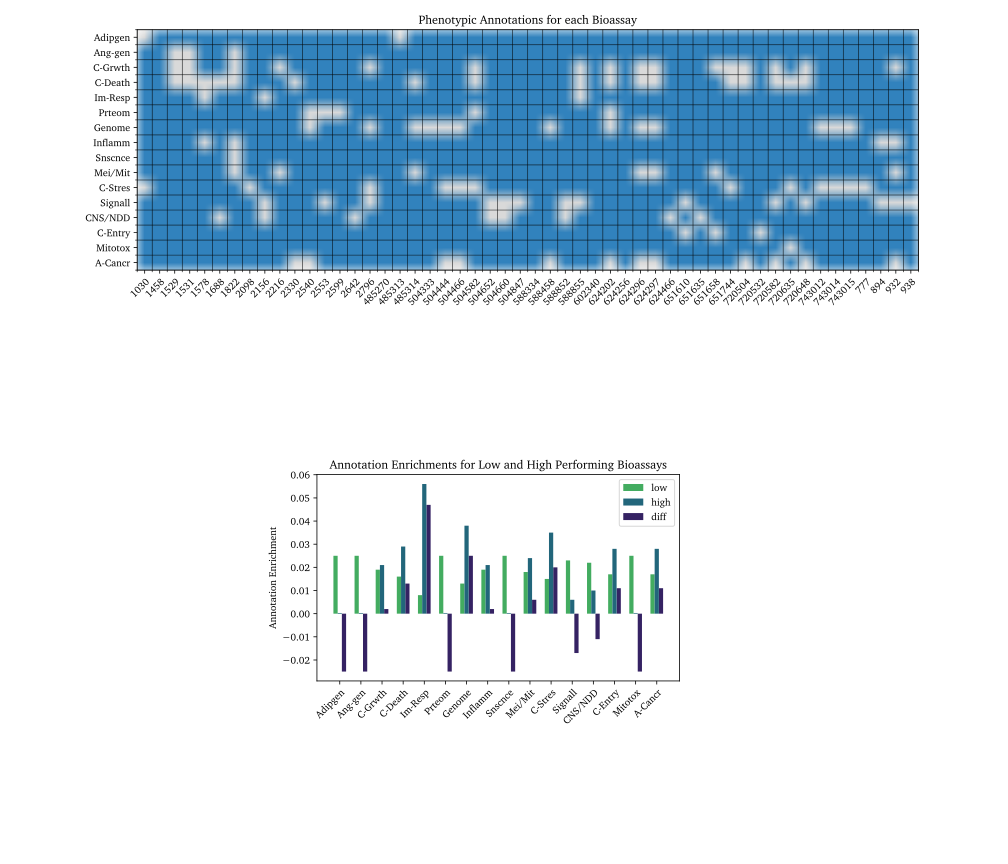
\includegraphics[width=\textwidth]{figures/phenotypic_annotations_corr.pdf}
	\caption[Phenotypic Terms That Can be Associated with Individual \acl{p} Assays]{Phenotypic terms that can be associated with individual \acl{p} assays. These terms were manually filtered from the descriptions of the \acl{p} assays available at \url{https://pubchem.ncbi.nlm.nih.gov/}. White fields correspond to presence and blue entries correspond absence of a term within an assay.}
	\label{fig:phenotypicsparse}
\end{figure}\noindent
Most importantly, the complete annotation matrix was created before the prediction performances were recorded and considered unbiased. This matrix allows testing for enriched annotations within \acl{hpa} and \acl{lpa} respectively.

The state for a phenotypic term within an assay can either be 'present' or 'absent', denoted by a \num{1} or \num{0}. To calculate the partial abundance of a given phenotypic term within a specific assay group $A_p^{xpa}$ the states for all relevant assays $s_p^{(a)}$ are summed up.
\begin{align}\label{eq:phenoabundance}
A_p^{^\text{lpa}} = \sum_{a}^\text{lpa}s_p^{(a)} \quad & A_p^{^\text{hpa}} = \sum_{a}^\text{hpa}s_p^{(a)}
\end{align}
The relative abundances or frequencies $a_p^{xpa}$ with an assay group can be calculated by dividing the partial abundances by the total abundance of the respective phenotypic term.
\begin{align}\label{eq:phenofreq}
a_p^{^\text{lpa}} = \frac{A_p^{^\text{lpa}}}{A_p^{^\text{lpa}}+A_p^{^\text{hpa}}} \quad & a_p^{^\text{hpa}} = \frac{A_p^{^\text{hpa}}}{A_p^{^\text{lpa}} + A_p^{^\text{hpa}}}
\end{align}
The enrichment of phenotypic term within an assay group needs to incorporate the total size of that group $N_{xpa}$. Therefore, the frequencies are divided by the corresponding group size to obtain the term related enrichment $R_p^{^\text{xpa}}$.
\begin{align}\label{eq:phenoenrichment}
R_p^{^\text{lpa}} = \frac{a_p^{^\text{lpa}}}{N_\text{lpa}} \quad & R_p^{^\text{hpa}} = \frac{a_p^{^\text{hpa}}}{N_\text{hpa}}
\end{align}
The resulting measure is the term frequency per assay and describes the enrichment of a phenotypic term within the corresponding assay group.\\
In \fref{tab:phenotypicenrichment} the enrichment for the \acl{hpa} and \acl{lpa} as well as the difference of the two is shown. A negative difference means that this phenotypic term is enriched in the \acl{lpa} and vice versa. It can be seen that phenotypic enrichment is positive for 'C-Grwth', 'C-Death', 'Im-Resp', 'Genome', 'Inflamm', 'Mei/Mit', 'C-Stres', 'C-Entry', and 'A-Cancr'. 'Im-Resp', 'Genome' and 'C-Death' are the three terms showing the highest enrichment.
\begin{figure}[H]
	\centering
	\includegraphics[width=0.9\textwidth]{figures/annotations_enrichment_corr.pdf}
	\caption[Annotations Enrichment in \acl{hpa} and \acl{lpa}]{Annotations Enrichment in \acl{hpa} and \acl{lpa} and the difference of the two. }
	\label{fig:annotenrich}
\end{figure}\noindent

\begin{table}[H]
	\footnotesize
	\centering
	\caption[Enrichment of phenotypic terms in \acl{hpa} and \acl{lpa}]{Enrichment of phenotypic terms in \acl{hpa} and \acl{lpa} and the difference between the two. A high number corresponds to a higher frequency of the corresponding term within the group of assays. The difference clarifies if the relative frequency is higher or lower in the \acl{hpa} and quantifies that enrichment in a comparable manner.}
	\label{tab:phenotypicenrichment}
	\begin{tabularx}{0.95\textwidth}{lllllllll}
		\toprule
		Group & Adipgen & Ang-gen & C-Grwth & C-Death & Im-Resp & Prteom & Genome & Inflamm\\
		\midrule
		low & 0.025 & 0.025 & 0.019 & 0.016 & 0.008 & 0.025 & 0.013 & 0.019\\
		high & 0.0 & 0.0 & 0.021 & 0.029 & 0.056 & 0.0 & 0.038 & 0.021\\
		diff & -0.025 & -0.025 & 0.002 & 0.013 & 0.047 & -0.025 & 0.025 & 0.002\\
		\midrule
		Group & Snscnce & Mei/Mit & C-Stres & Signall & CNS/NDD & C-Entry & Mitotox & A-Cancr\\
		\midrule
		low & 0.025 & 0.018 & 0.015 & 0.023 & 0.022 & 0.017 & 0.025 & 0.017\\
		high & 0.0 & 0.024 & 0.035 & 0.006 & 0.01 & 0.028 & 0.0 & 0.028\\
		diff & -0.025 & 0.006 & 0.02 & -0.017 & -0.011 & 0.011 & -0.025 & 0.011\\
		\bottomrule
	\end{tabularx}
\end{table}\noindent
From this analysis, it can be concluded that assays that probe endpoints related to these specified phenotypes exhibit higher predictive capability with \ac{cp} descriptors. The fact that genome integrity and \ac{dna}-repair scores a high value is also in agreement with the channel enrichment analysis. As shown in \fref{tab:channelstd}, the \ac{dna} channel has the highest ratio among all five.

\section{Gene Ontology Term Analysis}\label{sec:goterms}
% intro
\ac{go} terms are keywords referring to molecular functions or cellular processes associated with proteins. Each protein target is assigned a terminal \ac{go} term that is part of a hierarchical network. Hence every \ac{go} term can be associated with parent \ac{go} terms until the highest level of generalization is reached, leading to a tree of \ac{go} terms that are associated with each known protein.\\
% how they are applied here
%% discuss the six bioassays with no go terms
As an addition to the manually generated phenotypic annotations \ac{go} terms are generated for each bioassay which probes a protein target. Twelve \ac{p} assays do not probe protein targets, six of which are part of the \acl{hpa} group, and they are further discussed below. The terminal \ac{go} terms were obtained from \url{https://www.ebi.ac.uk/interpro} for each target and the entire hierarchy is extracted from \url{http://geneontology.org}. Since \ac{go} terms are hierarchical, a protein target with several unique terminal \ac{go} terms can have duplicate high order \ac{go} terms. For the analysis frequency information, i.e. how often a \ac{go} term appears within a given protein target is discarded. Afterwards, the relative abundance of \ac{go} terms within \acl{hpa} and \acl{lpa} are computed and compared. \ac{go} terms that are only present once throughout all assays are considered too rare to be included in comparative analysis and are therefore discarded. Since the \ac{go} terms directly describe mechanisms within the cell, a deeper understanding of the performances is anticipated. The concept is analogous to the manually developed phenotypic annotations because certain cellular mechanisms are anticipated to be more abundant within a certain group of assays.\\
% describe the figure
All \ac{go} terms found for the \num{52} \ac{p} assays and their relative abundances within high and \acl{lpa} are shown in \fref{fig:gotermabundances}. Roughly a third of the \ac{go} terms are associated with the \acl{hpa} most of which are also more abundant within \acl{hpa}. Furthermore, some of the \ac{go} terms are only present for \acl{hpa}. A majority of the \ac{go} terms found in total are present within protein targets of \acl{lpa}. A considerable amount of these is not present for \acl{hpa}.\\
% shortcomings
One problem that must be addressed concerns the small sample size. The \acl{hpa} only features six protein targets. That means the relative abundances are either \num{1/6}, \num{2/6}, etc. The \acl{lpa} feature this issue to a decreased extent. Therefore, this analysis has to be interpreted with a lack of data fidelity in mind. This approach is considered feasible if the number of biochemical assays is increased.
\begin{figure}[H]
	\centering
	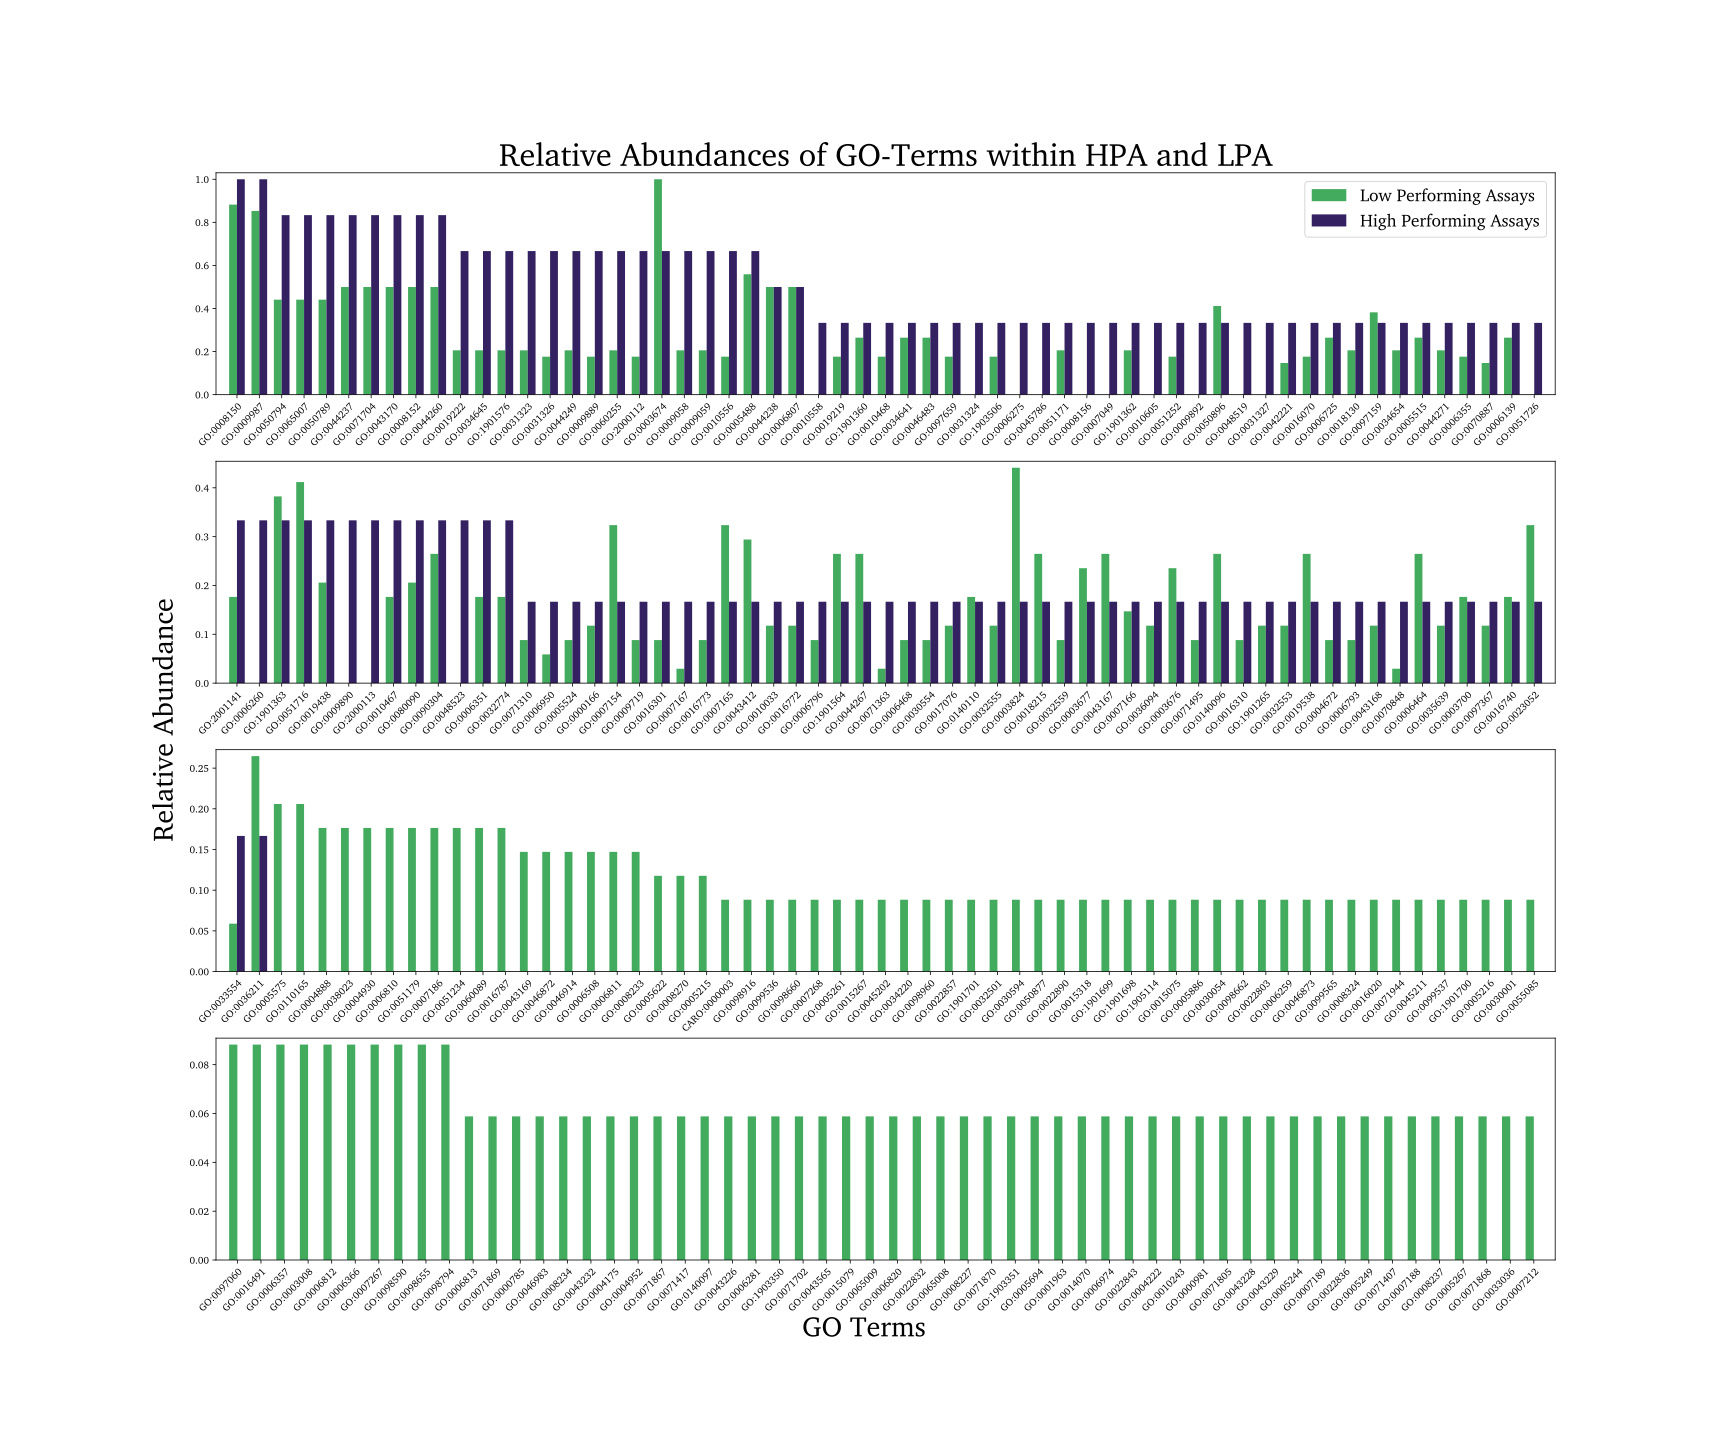
\includegraphics[width=\textwidth]{figures/go_frequencies.pdf}
	\caption[Relative Abundances of \ac{go} Terms in Each Assay Group]{Relative abundances of \ac{go} Terms in each assay group}
	\label{fig:gotermabundances}
\end{figure}
% conclusion
\fref{fig:gotermabundances} serves the sole purpose of visualization since it is only annotated with the \ac{go} term identifier and not with its description. The descriptions for \ac{go} terms enriched in high or \acl{lpa} can be found in \fref{tab:goterms} in the appendix. The \ac{go} terms for \acl{lpa} are very diverse and many instances related to synapses, ion transport and G-protein coupled receptors can be found. For \acl{hpa} the terms are enriched for metabolic and biosynthetic processes of macromolecules as well as the regulation and processing of \ac{dna} and \acs{rna}. This is in agreement with findings from \fref{sec:channelsresults}. In that section, the most important \ac{cp} features are analyzed for enrichment of channel variance. The \ac{dna} channel of \acl{hpa} is enriched by \SI{226}{\percent} compared to \acl{lpa}. Also in \fref{sec:phenotypicannotationsresults} the phenotypic annotation connected to genotoxicity and genetic regulation is highly enriched for \acl{hpa}. \ac{cp} descriptors seem to be particularly sensitive to bioassays primarily related to the regulation and processing of \ac{dna} and \ac{rna}. Nevertheless, the nucleus is the largest organelle in the cell. And the \ac{cp} descriptors are rooted in fluorescence microscopy which is dependend on signal resolution. Since most of the signal that is eventually imaged stems from the nucleus and is therefore related to \ac{dna} and \ac{rna}, this conclusion seems logical.\\
Additionally, the \acl{hpa} that do not probe gene products are inspected in further detail. The assays 651635, 651744, 720532, 743014, 743012 and 743015 are involved. Five out of these six probe complex cellular processes instead of single gene products. 651635 is the only assay that probes a gene product with no \ac{go} terms available by now. In \fref{sec:pubchem} the assay 720532 was explained in further detail as an example because it is the bioassay scoring the highest \ac{auc} via \ac{cp} descriptors. This assay probed the inhibition of virus entry by targeting cellular processes exploited by the virus. 651744 probes cytotoxicity within NIH3T3 cells via luminescence. 743012, 743014 and 743015 are parts of the same experiment where genotoxicity is screened for different mutants of the DT40 cell line.\\
Remarkably, five out of seven bioassays within \acl{hpa} probe for complex cellular processes. On the one hand, this hinders the annotation by \ac{go} terms. On the other hand, this indicates that \ac{cp} contains information that is particularly applicable for more complex cellular processes going beyond molecular functionality. This finding agrees with the richness in information that was also found by Simm \textit{et al.}\cite{Simm2017} when their \ac{cp} based model scored an \ac{auc} greater than \num{0.9} for \num{34} out of \num{600} assay. The authors do not specify what endpoints these assays probe in detail. The execution of an analysis similar to this one could validate the notion that \ac{cp} is most suitable for modelling complex biological mechanisms. 
	\chapter{Conclusion and Outlook}\label{sec:outlook}
% Nassiri and McCall
In this novel approach, the \ac{cp} data by Bray \textit{et al.} were used to predict certain \acl{p} assays that were selected for their relation to cytotoxicity. Nassiri and McCall\cite{Nassiri2018} used model performance as an indication for a common \ac{moa}. A similar approach is considered in this project. By comparatively analyzing performance metrics from an \ac{rfc} model among different descriptors, the relation of the bioassay to cellular morphology as captured by the \ac{cp} assay is inferred.\\
% results from comparative analysis
Within a comparative analysis of the different modelling approaches, twelve bioassay exhibit elevated predictive potential via \ac{cp} descriptors which were able to outperform \acp{ecfp} on nearly every metric. However, the specificity and sensitivity showed different behaviour in comparison to \ac{auc}, \acl{ba} and \ac{mcc}. The \ac{tpr} scored especially high for within the group of \acl{hpa}. That leads to the conclusion that \ac{cp} descriptors have a higher chance that a positively labelled compound is indeed positive. This characteristic is beneficial for toxicity prediction since the ability to correctly predict toxic (positive) compounds can prevent unnecessary testing and harm. The \ac{tnr} was found to be better predicted using either \acp{ecfp} or the feature engineered descriptor set. However, the \acl{sf} could not achieve an improvement over the individual predictive capabilities. It was also shown that \acp{ecfp} and \ac{cp} descriptors complement each other, which is in agreement with the findings from Lapins and Spjuth\cite{Lapins2019}. For drug safety projects, it is suggested to examine if \ac{cp} descriptors characterize the endpoint well. If so, feature engineering can be omitted for \ac{ml} approaches comparable to the one presented here. Predicting the \ac{tnr} is presumably better achievable via \acp{ecfp}.\\
% channel enrichment
A new enrichment metric developed from feature importance analysis is presented here. It measures the fluorescence channel-wise assay group standard deviation. This enrichment metric connects the results from feature engineering with cellular morphology, and it was found that for four out of five fluorescent channels, enrichment could be measured. This approach can be used as the first entry point when working with \ac{cp} data to categorize bioassays before prediction runs and focus on the assays that are estimated to be well characterized by \ac{cp} data.
% Lapins et spjuth
Lapins and Spjuth\cite{Lapins2019} used \ac{moa} and targets to annotate compounds in their work and used \ac{cp}, structural fingerprints and gene expression profiles as descriptors. A similar approach was chosen in the sense that structural fingerprints and \ac{cp} features were used as descriptors. Furthermore, their use of genetic information as a descriptor led to the idea that phenotypic annotations \ac{go} terms could be used to investigate the biological mechanisms responsible for performance differences within the \acl{p} bioassays. Opposite to Lapins et Spjuth\cite{Lapins2019}, the genetic information was not used as a descriptor but to further annotate the targets supplied by the \acl{p} assays.\\
The phenotypic annotations have been manually generated and connect the bioassays readouts to cellular processes (e.g. signalling, proteome regulation, genotoxicity etc.) that are likely to result in morphological changes. By calculating the phenotypic enrichment for \acl{hpa} and \acl{lpa}, it was found that endpoints that relate to genome integrity, \ac{dna}-repair, genotoxicity, cell-death, apoptosis, cell stress, toxins and immune response are generally better described by \ac{cp} descriptors.\\
Since the results agreed with the findings from the channel enrichment, the phenotypic analysis can be considered a confirmatory argument. However, its generalizability is hindered by its irreproducibility and critically imperfect knowledge. In an attempt to mitigate these shortcomings, the \ac{go} term analysis was conducted with results affirmative of the channel enrichment. Many \ac{go} terms found for the \acl{hpa} are connected to \ac{dna}, \ac{rna} and macromolecule synthesis. The caveat for \ac{go} term analysis stems from the relatively small sample size. Only six bioassays within the \acl{hpa} are probing gene products, therefore qualifying for this analysis. Nonetheless, it is suggested that \ac{go} terms should be included for a mechanistic and cellular understanding of the prediction performance when \ac{cp} data is in use, especially if a large number of endpoints are included in the analysis.
	

	

	\printacronyms[
	name = {Abbreviations}
	,sort = true
	,display = used
	,exclude=noprint]
	
	\selectlanguage{english}
	%\bibliography{master}
	%\bibliographystyle{achemso}
	
	% !TeX program = lualatex
\documentclass[
	ngerman,
	ruledheaders=section,%Ebene bis zu der die Überschriften mit Linien abgetrennt werden, vgl. DEMO-TUDaPub
	class=report,% Basisdokumentenklasse. Wählt die Korrespondierende KOMA-Script Klasse
	thesis={type=master},% Dokumententyp Thesis, für Dissertationen siehe die Demo-Datei DEMO-TUDaPhd
	accentcolor=1c,% Auswahl der Akzentfarbe
	custommargins=geometry,% Ränder werden mithilfe von typearea automatisch berechnet
	marginpar=false,% Kopfzeile und Fußzeile erstrecken sich nicht über die Randnotizspalte
	%BCOR=5mm,%Bindekorrektur, falls notwendig
	parskip=half-,%Absatzkennzeichnung durch Abstand vgl. KOMA-Script
	fontsize=11pt,%Basisschriftgröße laut Corporate Design ist mit 9pt häufig zu klein
%	logofile=example-image, %Falls die Logo Dateien nicht vorliegen
]{tudapub}
\geometry{a4paper,left=30mm,right=20mm,top=20mm,bottom=20mm,headsep=0.5cm}
\usepackage[english,plain]{fancyref}
%bessere optionen für das Cross referencing


%==Modifikationen=zu======Dokumentenformatierung===============================================================================================================

\makeatletter
\newcommand{\nobreakchap}{%
	\renewcommand\chapter{%
		\par\global\@topnum\z@
		\@afterindentfalse
		\secdef\@chapter\@schapter}
}
\newcommand{\normalchap}{%
	\renewcommand\chapter{%
		\if@openright\cleardoublepage\else\clearpage\fi
		\thispagestyle{\chapterpagestyle}%
		\global\@topnum\z@
		\@afterindentfalse
		\secdef\@chapter\@schapter}
}
\makeatother
%räumt durch den Befehl \nochapbreak die Möglichkeit nach einem \chapter keine neue Seite anzufangen
\renewcommand{\baselinestretch}{1.25}
%Modifikation des Zeilenabstands im Text
\renewcommand*{\thepage}{}									%Seitennummerierung manuell starten
%\numberwithin{equation}{section}
%Nummerierung der Formeln inkl. Kap.
%\numberwithin{figure}{section}
%Nummerierung der Abbildungen inkl. Kap.
%\numberwithin{table}{section}
%Nummerierung der Tabellen inkl. Kap.
%\usepackage{titlesec} % nicht kompatibel mit affidavit
%Abstand über Überschrift
%\titlespacing*{\chapter}{0pt}{-10pt}{0pt}
%schiebt die uberschrift nach oben um 10 pt. sieht besser aus
\usepackage{paralist}
%Paragraphen Erweiterung


%=========================Sprache=Symbole=und=Zeichen=========================================================================================================
\usepackage{amsmath}
% or simply amstext
\usepackage{amsfonts}
\usepackage[english]{babel}
%Sprache und Buchstaben aus Deutschland
\usepackage{courier}
%implementiert die Schriftart Courier
\usepackage[fleqn,tbtags]{mathtools}
%math. Umgebung
\usepackage{xurl}
%Angabe von URL mit \url{URL}
\usepackage[version-1-compatibility]{siunitx}
%si-Einheiten; Syntax und Mcaros nach Version 1
\DeclareSIUnit\molar{M}
%makes molar accesible as a unit of concentration
\sisetup{range-units = single}
%si-Einheiten-package
\sisetup{range-phrase = -}
%si-Einheiten-package "to" ersetzen "-"
\usepackage{upgreek}
%Griech. Buchstaben
\usepackage{chemformula}
%chemische Formeln in besserer Schreibweise
\usepackage{gensymb}
\usepackage{scalerel}
%=========================Verzeichnisse=======================================================================================================================
\usepackage[nottoc]{tocbibind}
%incorporates the bibliography into the toc 
\usepackage{bibgerm}
%Bibliographie in Deutscher codierung (umlaute) etc
\usepackage{achemso}
%Literaturverzeichnis im stil der American Chemical Society


%==Modifikationen=zu======Verzeichnisse=======================================================================================================================
\usepackage[stable]{footmisc}
%Zitieren von Fußnoten im stable Style 
%\bibliographystyle{plain}
%literaturverzeichnis auf deutsch
%\usepackage[printonlyused]{acronym} % http://ctan.org/pkg/acronym
%Abkürzungsverzeichnis [printonlyuse]=nur benutzte werden abgedruckt
\newcommand{\listofschemata}{\listof{schema}{List of Schemata}}
%definiert einen neuen Befehl zum erstellen von Schemataverzeichnis
\def\listschemaname{List of Schemata}
%definiert den Latex-Namen für das Schemataverzeichnis
\addto{\extrasngerman}{\renewcommand*{\listofschemata}{\listof{schema}{Verzeichnis der Schemata}}}
%legt den deutschen Namen fest für das Schemataverzeichnis
\addto{\extrasngerman}{\renewcommand*{\listschemaname}{Verzeichnis der Schemata}}
%legt den deutschen Namen fest für das Schemataverzeichnis


%=========================Abbildungen=etc=====================================================================================================================
\usepackage{rotating}
\usepackage{array}
%makes the new definition of column specifiers possible
\usepackage{etoolbox}
%kann zum speichern von Variabeln benutzt werden
\usepackage{filecontents}
%erlaubt das benutzen von Dateiinhalten im Zuge von tikzpicture (zum beispiel excel graphen)
\usepackage{float} 
%erlaubt das erstellen und definieren von floatobjekten
\usepackage{graphicx}
%Grafiken
\usepackage{pgfplots}
%Zusatzpackage für tikz
%https://texwelt.de/wissen/fragen/20061/farbverlauf-legende-tikz
%useful link for colormaps and their usage
\usepackage{pgfplotstable}
%irgendwas wegen linearer regression
\pgfplotsset{compat=1.13}
%not sure what dis does....
\usepackage{pdfpages}
%Integrieren von pdf
\usepackage{subcaption}
%erlaubt das erstellen von subfigures
\usepackage{svg}
%Vektorgrafiken
\usepackage{tabularx}
%Tabellen
\usepackage{tikz}
%Alle möglichen Arten von Grafiken
%\pgfrealjobname{osmoticcoefficient}
%modifikation zum tikz package. noetig fuer Externalizing
%refer to http://www.texample.net/media/pgf/builds/pgfmanualCVS2012-11-04.pdf Page 825ff
%'lualatex.exe -synctex=1 -interaction=nonstopmode -jobname=<dir>/<name> %.tex' into "options">"configure Texstudio"
\usepackage{wrapfig}
%textumflossende Floatobjekte
\usepackage{pdfpages}

%==Modifikationen=zu======Abbildungen=etc=====================================================================================================================
\usepackage[titles]{tocloft}
\cftsetindents{figure}{0em}{4cm}
\cftsetindents{table}{0em}{3.5em}
%Abbildungen und Tabellen
\usepackage{ragged2e}
%Beschriftung links bei Float-Objekten
\usepackage[justification=justified,format=plain,singlelinecheck=off,
labelfont=bf,font=footnotesize]{caption}
%Modifikation der Caption bei Float-Objekten
\renewcommand{\cfttabpresnum}{Tab. }
%Abkürzung Tabelle
\renewcommand{\cftfigpresnum}{Fig. }
%Abkürzung Abbildung
\settowidth{\cfttabnumwidth}{Fig. 10\quad}
%keine ahnung was das bringt
\settowidth{\cftfignumwidth}{Fig. 10\quad}
%keine ahnung was das bringt
\usepackage{booktabs}
%schönere Tabellen durch die befehle \toprule etc.
\usepackage{multirow}
%mehrere Tabellenzeilen in einer Spalte
%\renewcaptionname{ngerman}{\figurename}{Abb.}
%Abb.
%\renewcaptionname{ngerman}{\tablename}{Tab.}
%Tab. statt Tabelle
%\renewcaptionname{ngerman}{\figurename}{Fig.}
%\renewcaptionname{ngerman}{\tablename}{Tab.}
\newfloat{schema}{tbp}{los}[chapter]
%definition des float-objekts "Schema"
\floatname{schema}{Schema}
%Name des Floatobjekts "Schema"
\def\schemaautorefname{Schema}
%Referenzdefinition "Schema"
\floatstyle{plain}
%Festlegen des Floatstyles im Float-package
\newcolumntype{L}[1]{>{\raggedright\let\newline\\\arraybackslash\hspace{0pt}}m{#1}}
\newcolumntype{C}[1]{>{\centering\let\newline\\\arraybackslash\hspace{0pt}}m{#1}}
\newcolumntype{R}[1]{>{\raggedleft\let\newline\\\arraybackslash\hspace{0pt}}m{#1}}

%Formatierungen für Beispiele in diesem Dokument. Im Allgemeinen nicht notwendig!
\let\file\texttt
\let\code\texttt
\let\tbs\textbackslash

\usepackage{pifont}% Zapf-Dingbats Symbole
\newcommand*{\FeatureTrue}{\ding{52}}
\newcommand*{\FeatureFalse}{\ding{56}}

\pagenumbering{arabic}

\usepackage[smaller]{acro}
\DeclareAcronym{abc}{short=ABC,long=alpha bettick crisps}
\DeclareAcronym{ml}{short=ML,long=machine learning}
\DeclareAcronym{cp}{short=CP,long=cell-painting}
\DeclareAcronym{mlsmr}{short=MLSMR,long=Molecular Libraries Small Molecule Repository}
\DeclareAcronym{mlp}{short=MLP,long=Molecular Libraries Program}
\DeclareAcronym{er}{short=ER,long=endoplasmatic reticulum}
\DeclareAcronym{wga}{short=WGA,long=wheat germ agglutinin}
\DeclareAcronym{scc}{short=SCC,long=single-concentration-compound,tag=noprint}
\DeclareAcronym{dmso}{short=DMSO,long=dimethyl sulfoxide}
\DeclareAcronym{smiles}{short=SMILES,long=simplified molecular input line entry specification}
\DeclareAcronym{aid}{short=AID,long=assay identifier}
\DeclareAcronym{cid}{short=CID,long=compound identifier}
\DeclareAcronym{inchik}{short=InChI-key,long=international chemical identifier key}
\DeclareAcronym{p}{short=PubChem,long=PubChem,tag=noprint}
\DeclareAcronym{mbs}{short=MBS,long=\url{Metadata\_broad\_sample},tag=noprint}
\DeclareAcronym{prid}{short=prid,long=preprocessed raw image data,tag=noprint}
\DeclareAcronym{rid}{short=rid,long=raw image data,tag=noprint}
\DeclareAcronym{cmrds}{short=cmrds,long=combined ML-ready data set,tag=noprint}
\DeclareAcronym{ecfp}{short=ECFP,long=extended-connectivity fingerprint}
\DeclareAcronym{eset}{short=ECFP-set,long=ECFP-set,tag=noprint}
\DeclareAcronym{r}{short=r,long=radius,tag=noprint}
\DeclareAcronym{rfc}{short=RFC,long=random forest classifier}
\DeclareAcronym{cv}{short=CV,long=cross-validation}
\DeclareAcronym{kfcv}{short=KFCV,long=$k$-fold cross validation}
\DeclareAcronym{tpr}{short=TPR,long=true positive rate}
\DeclareAcronym{tnr}{short=TNR,long=true negative rate}
\DeclareAcronym{ba}{short=BA,long=balanced accuracy}
\DeclareAcronym{mcc}{short=MCC,long=Matthews correlation coefficient}
\DeclareAcronym{auc}{short=AUC-ROC,long=area under the ROC curve}
\DeclareAcronym{roc}{short=ROC-curve,long=receiver operating characteristic curve}
\DeclareAcronym{tp}{short=TP,long=true positive}
\DeclareAcronym{tn}{short=TN,long=true negative}
\DeclareAcronym{fp}{short=FP,long=false positive}
\DeclareAcronym{fn}{short=FN,long=false negative}
\DeclareAcronym{fpr}{short=FPR,long=false positive rate}
\DeclareAcronym{pca}{short=PCA,long=principal component analysis}
\DeclareAcronym{mrmr}{short=MRMR,long=minimal-redundancy-maximal-relevance criterion}
\DeclareAcronym{gi}{short=GI, long=gini impurity}
\DeclareAcronym{smote}{short=SMOTE,long=synthetic minority oversampling technique}
\DeclareAcronym{hpa}{short=hpa,long=high performing assays}
\DeclareAcronym{lpa}{short=lpa,long=low performing assays}
\DeclareAcronym{vsv}{short=VSV,long=vesicular stomatitis virus}
\DeclareAcronym{atxn}{short=ATXN2,long=Ataxin-2 gene}
\DeclareAcronym{sca2}{short=SCA2,long=spinocerebellar ataxia type 2}
\DeclareAcronym{moa}{short=MoA,long=mechanism of action,long-plural-form=mechanisms of action,short-plural-form=MoAs}
\DeclareAcronym{gcr}{short=GCR,long=glucocorticoid receptor}
\DeclareAcronym{hts}{short=HTS,long=high-throughput-screening}
\DeclareAcronym{iupac}{short=IUPAC,long=International Union of Pure and Applied Chemistry}
\DeclareAcronym{go}{short=GO,long=gene ontology}
\DeclareAcronym{sf}{short=SF,long=selected features}
\DeclareAcronym{af}{short=AF,long=all features}
\DeclareAcronym{dna}{short=DNA,long=deoxyribonucleic acid}
\DeclareAcronym{rna}{short=RNA,long=ribonucleic acid}

\RedeclareSectionCommand[beforeskip=0pt,
afterskip=2cm]{chapter}

\begin{document}
	\Metadata{
		title=Prediction of Cytotoxicity Related PubChem Assays Using High-Content-Imaging Descriptors from Cell-Painting,
		author=Luis Vollmers
	}
	
	\title{Prediction of Cytotoxicity Related PubChem Assays Using High-Content-Imaging Descriptors derived from Cell-Painting}
	\subtitle{A comparative study investigating the applicability of cell-painting data using machine learning methods and chemoinformatics tools}
	\author[L. Vollmers]{Luis Vollmers}
	\birthplace{Hannover}
	\reviewer{Prof. Dr. Katja Schmitz\and Dr. Andreas Bender}
	
	%\department{University of Cambridge}
	%\institute{Department of Chemistry}
	%\group{Bender Group}

	\addTitleBoxLogo*{\includegraphics[width=\linewidth]{figures/camlogo.jpg}}	
	
	\submissiondate{\today}
	\examdate{\today}
	
	\maketitle
	
	\affidavit% oder \affidavit[digital] falls eine rein digitale Abgabe vorgesehen ist.
	\tableofcontents
	
	\includepdf[pages=-]{daadtitlepage.pdf}
	\chapter{Summary}\label{sec:summary}
% introduction to toxicity
The pharmaceutical industry is centred around small molecules and their effects. Apart from the curative effect, the absence of adverse or toxicological effects is cardinal. However, toxicity is at least as elusive as it is important. A simple definition is: 'toxicology is the science of adverse effects of chemicals on living organisms'.\cite{Singh2018} However, this definition comprises several caveats. What is the organism? Where do therapeutic and adverse effects start and end? Even for the simplest organisms' toxicity, cytotoxicity, the mechanisms are manifold and difficult to unravel. Hence, it remains obscure which characteristics a compound has to combine to be labelled as toxic.\\
% introduction to cell painting
One attempt to illuminate these characteristics are novel \ac{cp} assays. For a \ac{cp} assay, cells are perturbed by libraries of small compounds, which might affect the cellular morphology before images are taken via automated fluorescence microscopy. Five fluorescent channels are used for imaging, and these channels correspond to certain cell organelles\cite{Carpenter2006}. Therefore \ac{cp} data contains information about cell structure variations caused by each compound. Which sub-information is actually valuable within these morphological fingerprints remains elusive. Therefore a significant part of the project presented here is dedicated to exploring the \ac{cp} data and their predictive capabilities comparatively. They will be compared against different descriptors for a variety of bioassays. The \ac{cp} data used in this project contains roughly \num{30000} compounds and \num{1800} features.\cite{Bray2017}\\
% introduce structural fingerprints
In chemistry, the structure determines the properties of a compound or substance. Therefore, apart from \ac{cp}, structural fingerprints are used as a benchmark descriptor set for comparison. In this project \acp{ecfp} were used to encode the compounds' structures as numerical features.\\
% introduction to pubchem assays
This work is concerned with morphological changes that correspond to toxicity. Thus, the \ac{cp} data were combined with toxicological endpoints from specific assays selected from the \acl{p} database. The selection process implemented a minimum number of active compounds, a size criterion and the occurrence of toxicologically relevant targets.\cite{Mervin2016}\\
% the procedure
After the selected assays were combined with each of their descriptors, machine learning models were trained, and their predictive power was evaluated against specific metrics. The predictions can be divided into four cycles. In the first cycle, the \ac{cp} data are used as descriptors, the second cycle used the structural fingerprints, and the third cycle used a subset of both. A rigorous feature engineering process selected the subsets. The last cycle skipped the feature engineering and combined all \ac{cp} and \ac{ecfp} descriptors into one large set of inputs.\\
% results
% metrics
The evaluation of the prediction metrics illuminates which strengths and shortcomings the morphological fingerprints feature compared to the structural fingerprints. It turned out that there are two groups of assays: those \acl{p} assays that are generally better predicted with \ac{cp} features and those that have higher predictive potential when using \ac{ecfp}. Additionally, it was revealed that \ac{ecfp} comprise higher specificity compared to \ac{cp} data which show higher sensitivity on the other hand. A high sensitivity means the prediction rarely mislabels a sample as negative (e.g. non-toxic) compared to the number of correctly labelled positive samples (e.g. toxic compounds.). Based on these results, \ac{cp} is better suited for toxicity prediction and drug safety evaluations since the mislabelled, positive compound can lead to expenses or even damage to health.\\
% channel enrichment
Furthermore, based on the data from fluorescent channels, an enrichment measure was introduced and calculated for the aforementioned two groups of \acl{p} assays. This enrichment connects predictive performance with cell organelle activity. The hypothesis was that \acl{p} assays, reliably predictable from \ac{cp} data, should exhibit increased enrichment, which was the case for four out of five fluorescence microscopy channels.\\
% phenotypic enrichment
As a next step, phenotypic terms were manually generated to categorize the different \acl{p} assays. These terms corresponded to cellular mechanisms or morphological processes and were generated unbiasedly. Nevertheless, they are subject to human error. The phenotypic annotations that are found to be enriched for successful modelling approaches might guide the pre-selection of bioassays in future projects. The enrichment analysis of phenotypic annotations detected that \acl{p} assays that could be well predicted via \ac{cp} data are related to immune response, genotoxicity and genome regulation and cell death.\\
% Go terms
Finally, the assays are assigned \ac{go} terms obtained from the \ac{go} database.\cite{Ashburner2000,Carbon2020} These terms comprise a controlled, structured vocabulary that explicitly describes the molecular function and biological processes of a given gene product. For \acl{p} assays associated with a protein target, the \ac{go} terms are collected. If an assay is particularly well predicted via \ac{cp} descriptors, the associated \ac{go} terms can relate this finding to cellular function. Even though the analysis with go terms suffers from a minimal sample size, it was found that \ac{cp} related assays usually correspond to processes concerning \ac{dna} and other macromolecules. This finding is in good agreement with the analysis of the channel enrichment as well as the phenotypic enrichment.
%% hier passt richtig gut ne abbildung hin vom generellen ablauf


\section{Zusammenfassung}
% Einführung in Pubchem-Assays
Diese Arbeit befasst sich mit zellul\"aren, morphologischen Veränderungen in Zusammenhang Toxizität. \ac{cp}-Daten wurden hierbei mit toxikologischen Endpunkten aus spezifischen Assays kombiniert, die aus der \acl{p}-Datenbank ausgewählt wurden. Das Auswahlverfahren implementierte eine Mindestanzahl von Wirkstoffen, ein Größenkriterium und das Auftreten toxikologisch relevanter Endpunkte.\cite{Mervin2016}\\
% das Verfahren
Nachdem die ausgewählten Assays mit ihren Deskriptoren kombiniert worden waren, wurden Modelle für \ac{ml} trainiert und ihre Vorhersagekraft anhand spezifischer Kenngr\"o{\ss}en bewertet. Die Vorhersagen können in vier Zyklen unterteilt werden. Im ersten Zyklus wurden die \ac{cp}-Daten als Deskriptoren verwendet, im zweiten Zyklus wurden strukturelle Merkmale verwendet, und im dritten Zyklus wurde eine Teilmenge beider verwendet. Ein ausgiebiger Feature-Engineering-Prozess wählte die Teilmengen aus. Im letzten Zyklus wurde das Feature-Engineering übersprungen und alle \ac{cp}- und \ac{ecfp}-Deskriptoren zu einem großen Datensatz zusammengefasst.\\
% Ergebnisse
% Metriken
Die Auswertung der Vorhersagemetriken zeigt, welche Stärken und Mängel die morphologischen Fingerabdrücke im Vergleich zu den strukturellen Merkmalen aufweisen. Es stellte sich heraus, dass es zwei Gruppen von Assays gibt: jene \acl{p}-Assays, die mit \ac{cp}-Daten im Allgemeinen besser vorhergesagt werden können, und jene, die bei Verwendung von \ac{ecfp} ein höheres Vorhersagepotential haben. Zusätzlich wurde gezeigt, dass \acp{ecfp} eine höhere Spezifität aufweisen als \ac{cp}-Daten, die andererseits eine höhere Empfindlichkeit zeigen. Eine hohe Empfindlichkeit bedeutet f\"ur eine Vorhersage, dass eine Probe im Vergleich zur Anzahl korrekt markierter positiver Proben (z. B. toxische Verbindungen) selten falsch als negativ (z. B. nicht toxisch) vorausgesagt wird. Basierend auf diesen Ergebnissen sind \ac{cp}-Daten besser für die Vorhersage der Toxizität und die Bewertung der Arzneimittelsicherheit geeignet, da eine falsch ausgewiesene positive Verbindung zu Kosten oder sogar zu Gesundheitsschäden führen kann. \\
% Kanalanreicherung
Darüber hinaus wurde basierend auf den Daten der Fluoreszenzmikroskopiekanäle eine Enrichment-Gr\"o{\ss}e eingeführt und für die oben genannten zwei Gruppen von \acl{p}-Assays berechnet. Diese Enrichment-Gr\"o{\ss}e verbindet die Vorhersageleistung mit der Aktivität der Zellorganellen. Die Hypothese war, dass \acl{p}-Assays, die zuverlässig aus \ac{cp}-Daten vorhersagbar sind, eine erhöhte Enrichment-Gr\"o{\ss}e aufweisen sollten, was bei vier von fünf Fluoreszenzmikroskopiekanälen der Fall war.\\
% phänotypische Anreicherung
Als nächster Schritt wurden phänotypische Kennw\"orter manuell generiert, um die verschiedenen \acl{p}-Assays zu kategorisieren. Diese Begriffe entsprachen zellulären Mechanismen oder morphologischen Prozessen und wurden unvoreingenommen generiert. Trotzdem unterliegen sie menschlichen Fehlern. Die phänotypischen Annotationen, die für erfolgreiche \ac{ml} Modelle angereichert sind, könnten die Vorauswahl von Bioassays in zukünftigen Projekten vereinfachen. Die Enrichment-Analyse phänotypischer Annotationen ergab, dass \acl{p}-Assays, die über \ac{cp}-Daten gut vorhergesagt werden konnten, mit Immunantworten, Genotoxizität und Genomregulation sowie Zelltod zusammenhängen.\\
% Go Begriffe
Schließlich werden den Assays \ac{go}-Begriffe zugewiesen, die aus der \ac{go}-Datenbank stammen. \cite{Ashburner2000, Carbon2020} Diese Begriffe umfassen ein kontrolliertes, strukturiertes Vokabular, das die molekulare Funktion und die biologischen Prozesse eines bestimmten Genprodukts explizit beschreibt. Für \acl{p}-Assays, sofern sie einem Protein Target zugeordnet sind, wurden die \ac{go}-Begriffe gesammelt. Wenn ein Assay über \ac{cp}-Deskriptoren besonders gut vorhergesagt wird, können die zugehörigen \ac{go}-Terme diesen Befund mit der Zellfunktion in Beziehung setzen. Obwohl die Analyse mit GO-Begriffen durch eine kleine Stichprobengröße eingeschr\"ankt sind, wurde festgestellt, dass \ac{cp}-bezogene Assays normalerweise Prozessen entsprechen, die \ac{dna} und andere Makromoleküle betreffen. Dieser Befund stimmt gut mit dem Enrichment der Fluoreszenzmikroskopiekanälen sowie den phänotypischen Annotationen überein.
%% hier passt richtig gut ne abbildung hin vom generellen ablauf
	\chapter{Introduction}\label{sec:introduction}
% Intro to drug development
Currently, pharmacological drug development focuses on well-established biochemistry based approaches to find and optimize new drugs. However, the challenges these methods face are manifold. High cost related to drug failure rates during various clinical trials and commercialization bottleneck the industry. Another important aspect is the occurrence of adverse drug reactions subjecting patients to hospitalization, possibly ending up fatal. Therefore, the pharmaceutical industry is not only facing high financial risks but also humanitarian issues that strain the trust-based relationship between the industry, physicians and patients.\cite{Katara2013}\\
% Computational drug development now
Academia demonstrated computational tools to be employable to many health industry challenges, such as costs of drug target validation, drug safety, and commercialization.\cite{Myers2001}\cite{Nelson2008} Albeit, chemo- and bioinformatics are novel and complex disciplines recently fostered by technological advancements in high-throughput methods and big-data analysis. Thus, the health industry does not yet benefit from promises like computer-aided identification of drugs and drug targets on a large scale.\\
% Cell Painting
New high-throughput methods and automated microscopy gave rise to the development of high-content imaging, which is frequently used to record small compound perturbations inflicted on biological systems. High-content-imaging applies up to six fluorescent dyes allowing to portray up to five different compartments per cell simultaneously. This method also referred to as \acf{cp} captures compound perturbed biological systems and automatically resolves cellular characteristics.  Computational models can interpret these in the context of a morphological fingerprint (or \ac{cp} feature vectors).\cite{Bray2017,Simm2017}\\
% Cell Profiler
The raw images from high-content imaging are processed, mostly by the software CellProfiler\cite{Carpenter2006} which extracts up to \num{1800} numerical features per image (e.g. nucleus shape, \ac{er} texture, etc.). Features from \ac{cp} assays can be interpreted as a morphological fingerprint, unique for each compound.\cite{Simm2017} By now, many different \ac{cp} assays have been conducted. A widely used \ac{cp} data set was generated by Bray \textit{et al}.\cite{Bray2016} The images were recorded with sixfold fluorescence staining for imaging five crucial cellular organelles (further information see \fref{sec:cpassay}).\cite{Bray2017} The concept of \ac{cp} is visualized in \fref{fig:cpprocess}.\\
\begin{figure}[H]
	\centering
	\includegraphics[width=\textwidth]{figures/cp_process.png}
	\caption[Visualization of a \ac{cp} Assay]{Visualization of a \ac{cp} assay. First cellular images are generated by fluorescence microscopy, then cellular objects and compartments are recognized by CellProfiler from which a large data table is generated containing the morphological fingerprint for each compound. Figure from Rohban \textit{et al.} and Carpenter \textit{et al.}, modified.\cite{Carpenter2006,Rohban2017}}
	\label{fig:cpprocess}
\end{figure}\noindent
% Gustafsdottir
Recently, Gustafsdottir \textit{et al.}\cite{Gustafsdottir2013} used \ac{cp} data to link morphological states to \acp{moa} via gene expression data. Hierarchical clustering was used to find clusters of compounds, addressing the same set of genes and, therefore, the same biochemical pathway. The results obtained from this \ac{cp} based approach mirrored the findings in the literature, which showed that \ac{cp} data is directly correlated to cellular pathways responding to compound perturbations.\\
% Nassiri and McCall
Nassiri and McCall\cite{Nassiri2018} used different \ac{cp} assay data\cite{Wawer2014a} and compound perturbed gene expression data in the context of machine learning methods. They used a LASSO model to predict cell morphological features against similar gene expression profiles. In-depth analysis of the results revealed strong model predictiveness among compounds that steer gene expression in the same direction, suggesting common \acp{moa}. In addition to linking \ac{cp} data to \acp{moa} they revealed direct relations between compounds' \acp{moa} based on machine learning model performance.\\
% Rohban et al
Furthermore, Rohban \textit{et al}.\cite{Rohban2017} transduced U-2 OS cells with lentiviral particles carrying cDNA constructs for gene overexpression.\cite{Wiemann2016,Yang2011} In their approach, they conducted a \ac{cp} assay to annotate the overexpressed genes with morphological fingerprints (numerical \ac{cp} features). After calculating the Pearson correlation between each morphological fingerprint, they used hierarchical clustering resulting in \num{25} clusters for \num{110} overexpressed genes. The clusters generated from the \ac{cp} data agglomerated genes that correspond to similar or identical pathways showing that genes can be connected using relatively inexpensive \ac{cp} assays. Furthermore, they predicted an unknown relationship between the Hippo- and NF-$\kappa$B-pathway.\\
% lapins and Spjuth
Lapins and Spjuth\cite{Lapins2019} annotated compounds of the \ac{cp} data from Bray \textit{et al.}\cite{Bray2017} and from the CMap\cite{Subramanian2017} (gene expression profiles) with their \ac{moa} or target protein. The information about the compound-wise \ac{moa} and targets was obtained from the Drug Repurposing Hub or the Touchstone database. In total, they annotated \num{1484} compounds present in \ac{cp} and CMap data with \num{234} \acp{moa} or targets. As the third set of descriptors, structural fingerprints were generated. For several targets and \acp{moa} a trained \ac{rfc} could present significant discriminatory power (\acs{auc}>\num{0.7}). Furthermore, it was found that the three different descriptors were complementary to a certain degree, each excelling at different \acp{moa} or targets. Lapins and Spjuth not only showed that \ac{cp} data could be used to predict compound's \ac{moa} but also that a combination with other identifiers is likely to enhance their applicability domain.\\
% Simm et al
Simm \textit{et al}.\cite{Simm2017} studied a \ac{cp} assay specifically designed for \ac{gcr} nuclear translocation. After treating H4 brain neuroglioma cells with \num{524371} compounds, hydrocortisone was added to stimulate \ac{gcr} translocation. Next, the treated cells were stained, imaged and processed analogously to the work of Gustafsdottir \textit{et al.}\cite{Gustafsdottir2013} The \num{524371} compounds were not only annotated with morphological information, but also with target activity information from \num{600} biochemical assays. Noticeably, most compounds were covered in few assays only, amounting to a fill rate of \SI{1.6}{\percent}. From this sparse activity matrix, they built a \ac{ml} model with \ac{cp} data as side information to predict all labels within the activity matrix. They evaluated the discriminatory power of their model and \num{34} bioassays (out of \num{600}) showed high predictivity (\acs{auc}>\num{0.9}). One of the assays was part of an ongoing discovery project. Within this assay, the highest-ranking \num{342} compounds, by matrix factorization, were experimentally tested. \num{141} ($41.2\%$) of these resulted in submicromolar hits which means a \num{60}-fold enrichment over the initial \ac{hts}. Another assay with an \ac{auc} greater \num{0.9} was part of an ongoing drug discovery project and could achieve a \num{250}-fold hit enrichment over the initial \ac{hts} in an analogous way. Their work presented \ac{cp} data as highly informative descriptors that might be repurposed for the prediction of sparse activity matrices. Additionally, they demonstrated their potential in ongoing drug discovery projects.\cite{Simm2018}\\
% working in data science and with CP
Data science in drug development and pharmacology has great potential. However, some caveats require carefulness when working with \ac{cp} data to access drug safety. The first one is imbalanced data. An assay testing compounds on a potential target will always feature fewer actives than inactive. Chawla \textit{et al.}\cite{Chawla2002} proposed a technique that mitigates this effect called \ac{smote}. This technique allows generating synthetic data that fit into the distribution of the real data points. Another obstacle is the high dimensionality of \ac{cp} data. Only a comparably small number of features contains most of the information necessary to predict a given target. Thus, statistical tools are applied for sophisticated feature selection in \ac{cp} studies. A \ac{cp} data set containing too many features is bound to overfit the data and give overoptimistic predictions on the test set without generalizing particularly well. The project above of Rohban \textit{et al.}\cite{Rohban2017} tackled this problem by \ac{pca}. Thereby reducing the number of features from \num{2769} to \num{158} which comprise most of the variance.\\
% about this work
In this explorative \ac{ml} project, targets obtained from bioassays published on \acl{p} are predicted with regard to descriptors from the \ac{cp} data set of Bray \textit{et al.}\cite{Bray2017}. The \acl{p} assays are selected based on their relation to targets presumably contributing to cytotoxicity.\cite{Mervin2016} The results are compared to the small molecules' structural fingerprints, and the performance metrics are analyzed extensively. From this analysis, conclusions can be drawn, whether and when to use \ac{cp} data. Insights gained from this project might guide future decision making when it comes to the prediction of biological endpoints.
	\chapter{Scientific Aim}\label{sec:scientificaim}
% most general notion of the scientific aim
This project aims to generate heuristics that simplify working with \ac{cp} data. Generally, \ac{cp} data can be used as descriptors to predict targets obtained from compound associated biochemical readouts. The mechanistic relation between a biochemical readout and its predictivity via \ac{cp} descriptors is poorly understood. Therefore, this work aims at understanding the results obtained from \ac{rfc} prediction and linking the results to cellular mechanisms and the concept of cytotoxicity.\\
% specify what that means
Conceptually, this means finding bioassays whose endpoints are related to toxicity for annotating the \ac{cp} descriptors. Since this is a comparative approach, structural fingerprints (\acp{ecfp}) are used as another descriptor set. Both annotated data sets are entered into an \ac{ml} model, and this model's discriminatory power is evaluated using generic statistical metrics. Another model is trained using the combined set of descriptors which is evaluated analogously.\\
% specify the approach taken in this work
The detailed procedure starts by preprocessing the \ac{cp} raw image data into a \ac{ml}-ready data frame. Next, the bioassays are selected from \acl{p}\cite{Kim2020}, based on size and their relation to cytotoxicity. Every bioassay data frame is combined with the \ac{cp} data frame to obtain annotated sets containing inputs as well as targets for prediction.\\
For comparison, structural descriptors are generated for all data sets using \texttt{sklearn}-funtionalities\cite{Pedregosa2012}. To this end, the annotations in all data sets are highly imbalanced, comprising mostly samples labelled as inactive. Herein, this problem is tackled by applying \ac{smote} to the data sets in combination with undersampling of the majority label (inactive).\\
Two \ac{rfc} models are trained on each data set, and their predictive power is evaluated. Furthermore, to examine if one descriptor's shortcomings can be mitigated by the other, selected features from both descriptors are combined, and another model is trained and evaluated. Since there is no apparent way to select features manually, statistical methods can be used to conduct features selection meaningfully. \ac{pca}, \ac{mrmr} and random forest feature importance are applied to score and select features from each set of descriptors for merging. Eventually, a fourth \ac{rfc} model is trained and evaluated using the complete feature sets from both descriptors.\\
Based on the prediction evaluation and feature selection process, a rigorous analysis is conducted to explain the results with respect to cellular morphology and cytotoxicity. The focus lies in detecting and analyzing prediction similarities and dissimilarities between either descriptor sets, bioassays or groups characterized by their performance. Thereby, patterns can be detected that transform into heuristics which facilitate the application of \ac{cp} data to \ac{ml} problems in the future.
	\chapter{Theoretical Background}\label{sec:background}
\section{Simplified Molecular Input Line Entry Specification - SMILES}\label{sec:smiles}
The \ac{smiles} refer to a specific formalism to generate identifiers for chemical compounds that are suited for chemists and computational input. The identifier, in this case, is deduced from a two-dimensional graph of the chemical structure. The result is a series of characters that contain mostly alphanumeric symbols, brackets and some other symbols. The selection of those symbols follows a specific order and a specific set of rules. The set of rules addresses six categories: atoms, bonds, branches, cyclic structures, disconnected structures and aromaticity. Also, \ac{smiles} considers stereochemical information. However, that is not mandatory since the initial approach to \ac{smiles} covers solely two-dimensional information.\cite{Weininger1988}
Atoms are labelled by their element symbol. All elements of a \ac{smiles} string are written in square brackets with the exceptions of the organic subset, i.e. B, C, N, O, P, S, F, Cl, Br, and I. Hydrogen atoms have further specifications. They can either appear implicitly with members of the organic subset. In that case, the remainder of the lowest valence is filled with hydrogen atoms. For example, [C] refers to \ch{CH4}. Explicit notation of hydrogen atoms occurs when they are attached to an element that is not part of the organic subset. Given a metal M, the nomenclature of four hydrogen atoms attached to that metal is [MH4]. Hydrogen can also be mentioned on its own in brackets [H], e.g. in its molecular form \ch{H2}. Charges are represented with a plus or minus with their respective count inside a bracket.\cite{Weininger1988}
Bonds within the \ac{smiles} nomenclature are omitted if they are either aromatic or single covalent bonds. Double bonds are represented with '\ch{=}', and triple bonds are represented by '\#'. Ionic bonds are not explicitly denoted by the \ac{smiles} algorithm. An ion pair is written as two disconnected structures with formal charges to them. Tautomeric bonds are not explicitly denoted either. One of the possible structures is translated into the \ac{smiles} string, be it the enol or keto variation.\cite{Weininger1988}\\
Branches are depcited in parenthesis. 5-Methyl-4-(2-methylpropyl)-4-(propan-2-yl)hept-1-ene is an example of nested branching using nested parenthesis. The name of the structure is according to the convention of \ac{iupac}\cite{2014a}. The structure and \ac{smiles} is shown in \fref{fig:branching}.
\begin{figure}[H]
	\centering
	\includegraphics[width=0.9\textwidth]{figures/branch.pdf}
	\caption[Demonstration of a Branching Structure with SMILES]{On the left, side a model compound is shown as an example of nested branching in \ac{smiles}. On the right, the \ac{iupac} name and its \ac{smiles} string are shown. The \ac{smiles} string features parenthesis that imply branching and nested branching.\cite{Weininger1988}}
	\label{fig:branching}
\end{figure}\noindent
Cyclic structures are written linearly by breaking a single or aromatic bond within the cycles. Next, the broken bonds are arbitrarily labelled by writing the formerly connecting elements right in front of a number assigned to the broken bond. An illustrating example is shown in \fref{fig:cycle}.
\begin{figure}[H]
	\centering
	\includegraphics[width=0.5\textwidth]{figures/cycle.pdf}
	\caption[SMILES string of a Cyclic Structure]{Cyclohexane as an example for a cyclic structure. First, the explicit hydrogens are exchanged for implicit ones, and the ring is linearized by conceptually breaking a bond implied by the dashed line. The carbons connected by the dashed line are being labelled, and the resulting \ac{smiles} string is shown below the right-hand structure.\cite{Weininger1988}}
	\label{fig:cycle}
\end{figure}\noindent
A single atom can be part of multiple rings which is then accounted for by using two or three single digits in sequence. However, for structures with more than ten rings, double digits are separated with a prefacing per cent sign. Also, a single digit can be reused for multiple broken bonds without creating ambiguity. A \ac{smiles} string is read from left to right, and a ring closes on the first repetition of a respective digit. Cubane is an example that has multiple rings. In \fref{fig:cycles} the generation of a \ac{smiles} string is shown with the usage of the digit '1'. \cite{Weininger1988}
\begin{figure}[H]
	\centering
	\includegraphics[width=0.7\textwidth]{figures/cubane.pdf}
	\caption[SMILES String that Resembles Multiple Cycles within the Same Molecule]{Cubane as an example of a structure that has multiple cycles. On the left, the structure is shown without explicit hydrogen atoms. In the middle picture, the bonds that are artificially broken to linearize the molecule for the \ac{smiles} string are shown in dashes. On the very right, the skeleton structure resembles the \ac{smiles} string, that is written below the molecular representations.\cite{Weininger1988}}
	\label{fig:cycles}
\end{figure}\noindent
A \ac{smiles} string is read from left to right, and a ring closes on the first repetition of a respective digit. Disconnected structures are written as individual \ac{smiles} strings separated by a comma. \cite{Weininger1988}\\
Aromaticity is denoted by writing the atoms that are part of an aromatic cycle in lower case letters. Aromaticity is detected by applying an extended definition of H\"uckel's rule. Another noteworthy convention is the treatment of aromatic nitrogen atoms. A nitrogen atom that is embraced by two aromatic bonds has no valency left per default. However, for aromatic nitrogen that is connected to a hydrogen atom, the hydrogen atom is specified as shown in \fref{fig:nitrogen}.\cite{Weininger1988}
\begin{figure}[H]
	\centering
	\includegraphics[width=0.9\textwidth]{figures/aromaticnitrogen.pdf}
	\caption[Specifications for Aromatic Nitrogen within the \ac{smiles} algorithm]{Different instances of aromatic nitrogen. Notice that the \ac{smiles} string of pyrrole contains an additional hydrogen atom that preceded the aromatic nitrogen. The aromaticity of an atom is denoted by writing it in lower case letters.\cite{Weininger1988}}
	\label{fig:nitrogen}
\end{figure}\noindent
Furthermore, the \ac{smiles} algorithm introduces a convention for labelling double bond configurations and chirality. The double bond configuration is indicated by placing '/' or '\textbackslash' between the atom constituting the double bond and their subsequent bonding partners. The indicators can be understood as a single bond type that gives information about their relative orientation. An example for (Z)-1,2-difluoroethene and (E)-1,2-difluoroethene is given in \fref{fig:doublebond}.\cite{smilesmanual}
\begin{figure}[H]
	\centering
	\includegraphics[width=0.7\textwidth]{figures/doublebond.pdf}
	\caption[Example of Double Bond Configuration in \ac{smiles} Notation]{Example of double bond configuration in \ac{smiles} notation. On the left (Z)-1,2-difluoroethene is shown and on the right is (E)-1,2-difluoroethene with their \ac{smiles} notation. Both notations shown for each structure are valid.\cite{smilesmanual}}
	\label{fig:doublebond}
\end{figure}\noindent
Chirality is assigned to chiral tetrahedral centres and any other chiral centre, e.g. allene-like or square planar centres. Herein, the \ac{smiles} notation is explained in the context of tetrahedral chirality centres, which is the most straightforward instance of chirality in organic chemistry. A chiral centre can not be the terminal node in a molecular representation since a terminal node is either only connected to hydrogen atoms if any at all. With that in mind, the convention for tetrahedral chirality is most easily explained by investigating an example which is (1S)-1-chloro-1-fluoroethan-1-amine which can be seen in \fref{fig:enantio}. The whole molecule is viewed along the CC-bond. Necessarily, the \ac{smiles} string contains the central C-atom's binding partners in a specific order. This sequence can either correspond to the clockwise or anticlockwise binding partners' order when the molecule is viewed along the CC axis. Should the order be anticlockwise, an '@' is inserted after the central C-atom in brackets. The '@' is a visual mnemonic since it depicts an anticlockwise rotation around the central circle. For a clockwise order, '@@' is used instead of a single '@'.
\begin{figure}[H]
	\centering
	\includegraphics[width=0.8\textwidth]{figures/tetrachiral.pdf}
	\caption[Example of Enantiomere \ac{smiles} Strings]{Example of enantiomer \ac{smiles} strings.\cite{smilesmanual} Both molecules are pictures in the same way. Above each depiction is the name of the chemical formula followed by a schematic. The eye indicates the point of view along the CC axis. The resulting view of the structure is shown on the right of each subfigure. Written below are two equally adequate \ac{smiles} strings for each structure.}
	\label{fig:enantio}	
\end{figure}\noindent
%
%
\section{Canonical SMILES}\label{sec:cansmiles}
In general, \ac{smiles} strings do not claim to be unique identifiers. There are many equivalent options to generate a \ac{smiles} string for a given structure. Nowadays, computational biochemical research accesses structures from many different sources and databases, making the requirement of a unique identifier evident. The \ac{smiles} notation was developed with this objective in mind. So-called canonical \ac{smiles} strings fulfil this objective. They are based on the same set of rules described in \fref{sec:smiles}. The algorithm can be partitioned into two parts: the CANON part and the GENES part. The CANON part labels the atoms of the molecular structure canonically, i.e. a unique way based on the structural topology. The GENES part generates the unique \ac{smiles} from the aforementioned rule set (see \fref{sec:smiles}) and the canonical labelling.\cite{Weininger1989}\\
For finding a unique way of labelling atoms in a molecule, invariant structural properties are necessary. Thus, five properties are considered atomic invariants. Those would be (1) the number of connections, (2) the number of non-hydrogen bonds, (3) the atomic number, (4) the sign of the charge and (5) the number of attached hydrogens. They are called 'invariant' because they are invariant to atomic order changes within a structural notation, and they are exchangeable as long as this principle is not violated. The numbers in the parenthesis in front of each property correspond to a pre-defined prioritization.
In summary, the atomic invariants assign five integers to every atom in a molecule. The so-called individual invariant can be obtained by simply combining these integers in order of their prioritization. Given the methyl carbon of 2-(acetyloxy)benzoic acid in \fref{fig:canonicallabelling} with the individual invariant 110603. From this individual invariant, it can be concluded that this atom has 1 connection, 1 bond to a non-hydrogen neighbour, an atomic number of 06, 0 charge and 3 attached hydrogen atoms.
Other atomic properties like isotopic mass and local chirality can be added if these six properties are not sufficient to discriminate all distinguishable nodes from each other. It is noteworthy that some nodes are symmetric and require a tie-breaking function for absolute uniqueness (see next paragraph).\cite{Weininger1989}\\
After assigning every atom an individual variant, those are compared among all constituting atoms and are ranked by magnitude. The final atom labels depend on the topology, as well. Therefore, the nodes (atoms) rank is extended by its corresponding prime (for 1, 2, 3, the corresponding primes are 2, 3, 5). The so-called new invariant is obtained by multiplying the corresponding primes of all neighbours for every atom. Afterwards, ranks are assigned again, based on their current rank and new invariant. The procedure is repeated iteratively until the combined invariant is not changing anymore. Should there be constitutionally symmetric nodes present in the molecular graph, it becomes necessary to break ties since the symmetric groups make it impossible to find a ranking that offers a completely ordered set of nodes necessary for finding a canonical \ac{smiles} representation. For tie-breaking, all ranks are doubled, and the first instance of an asymmetric node is decremented by one. The resulting node ranking is considered a new invariant set that goes through the aforementioned iterative process of corresponding prime multiplication until it is no longer changing. After every rank is of the combined invariant is unique and not changing upon further iteration, the uniquely ordered ranking has been accomplished.\cite{Weininger1989} The canonical labelling process for 2-(acetyloxy)benzoic acid is shown in \fref{fig:canonicallabelling}.
\begin{figure}[H]
	\centering
	\includegraphics[width=0.9\textwidth]{figures/canonical_labelling.pdf}
	\caption[Canonical Labelling with 2-(Acetyloxy)Benzoic Acid]{Canonical labelling with 2-(acetyloxy)benzoic acid. Every row corresponds to consecutive iterations of the CANON algorithm. The blackboard bold $\mathbb{P}$ denotes finding corresponding primes. The greek letter $\Pi$ denotes taking the prime products of all atoms, and the hashtag denotes atoms' ranking. Bold numbers denote ranks that reached invariance.}
	\label{fig:canonicallabelling}	
\end{figure}\noindent
THE GENES part of the algorithm can utilize the uniquely ordered ranking to chose the start node and prioritize at branching points, etc. As an entry point for the generation of canonical \ac{smiles}, the node with the lowest ranking is chosen. Branching decisions are made in the same fashion, i.e. the branching option with the lowest rank is chosen and followed until a dead end has been reached. A special rule applies when branching into a ring with a double or triple bond. To avoid opening the ring at any multi-bond, the algorithm will always branch towards the multi-bond. Also, the ring-opening digits must be in the order of ring-opening nodes.\\
Conclusively, a unique \ac{smiles} string can be assigned by first generating a unique invariant rank for every node that incorporates invariant atomic properties and topological information and then using these ranks as decision indicators for branching and cycles.\cite{Weininger1989}
%
%
\section{Extended-Connectivity Fingerprints}\label{sec:extendedconnectivityfingerprints}
The \ac{ecfp} is a structural fingerprint that was developed to capture molecular features relevant for molecular activity.\cite{Rogers2010} \acp{ecfp} are also commonly referred to as Morgan-fingerprints since their development is partially based on the Morgan-algorithm which pursues rigorous canonicalisation similar to the CANON algorithm in \fref{sec:cansmiles}.\cite{Morgan1965} 
The procedure of the algorithm can be distinguished into two parts: the initialization (or zeroeth iteration) and the iteration process.\\
For initialization, all atoms in the molecule are given an identifier that is computed from six atomic invariants, similar to the ones in \fref{sec:cansmiles} canonical \ac{smiles} algorithm (number of connections, number of bonds, atomic number, atomic mass, atomic charge, number of attached hydrogens).\cite{smilesmanual} However, a seventh invariant is taken into account: whether the atom is part of at least one ring structure. A hashing algorithm maps the atomic invariants to a 32-bit integer. Any functional hashing algorithm that reproducibly maps the input onto a 32-bit integer is a sensible choice since the only requirement is that a variant is uniquely mapped to the same 32-bit integer every time it is hashed. The 32-bit integer is also referred to as the core identifier. Within the initialization step, it corresponds to a substructure that contains information about one atom and its bonds and is appended to a list called \acl{eset}. After completion of the algorithm, the \acl{eset} is equal to the fingerprint.\cite{Rogers2010} Therefore, the result of the initialization are a set of core identifiers [$c^{(0)}_0,c^{(0)}_1,c^{(0)}_2,...,c^{(0)}_n$]. The core identifier for atom 1 of the initialization (zeroeth iteration) would be $c^{(0)}_1$.\\
After the initialization the first iteration starts by randomly picking an atom, let that be atom 4. Next, the iteration number (1) and the core identifier, $c^{(0)}_4$, are appended to a temporary list. Afterwards, the neighbouring core identifiers are appended to the temporary list together with their respective bond order. $b_{4j}$ denotes the bond order between atom 4 and its neighbour, $j$. The bond order can either be 1, 2, 3 or 4 for aromatic bonds. Let the resulting temporary list have the following format $[1,c^{(0)}_4,b_{34},c^{(0)}_3,b_{45},c^{(0)}_5,b_{46},c^{(0)}_6]$. In this example the temporary list comprises eight entries which are inputted into a hashing function that returns a 32-bit integer. This integer is the core identifier of atom 4 for, $c^{(1)}_4$. Once this process is completed for every atom, all core identifiers are updated to the new core identifier simultaneously and are appended to the \acl{eset}. The temporary lists are being discarded. After iteration 1, the \acl{eset} comprises of the elements $[c^{(0)}_0,...,c^{(0)}_n,c^{(1)}_0,...,c^{(1)}_n]$.\cite{Rogers2010}\\
The second iteration is conducted in the same way as the first iteration. However, the core identifier of $j$ of the first iteration contains information about its surrounding cores and their bonds. Therefore, information from up to two bonds is incorporated into the second iteration's core identifiers, $c^{(2)}_j$. Thus, from iteration to iteration, the core identifiers can be understood as the core atom within a larger and larger structural neighbourhood. $c^{(0)}_j$ is a 32-bit integer that encodes the atom $j$ and its adjacent bonds. $c^{(1)}_j$ is a 32-bit integer that encodes atom $j$, its neighbouring atoms within one bond length, their bond orders and their adjacent bonds, and so on.\cite{Rogers2010}\\
After the specified number of iterations is completed, duplicate 32-bit integers are removed from the \acl{eset} since they encode for the same subtructure. Butyramide is shown in \fref{fig:butyramideecfp} as a conceptual example of fingerprint generation.\cite{Rogers2010}
\begin{figure}[H]
	\centering
	\includegraphics[width=0.6\textwidth]{figures/butyramide_ecfp.pdf}
	\caption[Fingerprint Iterations with Substructures for One Atom]{Fingerprint iterations with substructures for one atom. Atom 4 of butyramide iterated, denoted by the red circles. The smallest circle denotes initialization of atom 4, resulting in $c^{(0)}_4$ only containing information about the core atom and adjacent bonds. The first iteration is denoted by the intermediate circle and results in $c^{(1)}_4$. The second iteration is denoted by the outer circle and results in $c^{(2)}_4$.}
	\label{fig:butyramideecfp}
\end{figure}
So far \acl{eset} contains 32-bit identifier. A substructure could be encoded by the integer, e.g. 1559650422, which would correspond to an "on" bit within a bit set of $2^{32}$ bits. Since a hash space of $2^{32}$ is quite vast, the 32-bit integers are usually mapped onto a vector of 1024 (or 2048) bits by yet another hashing algorithm. Even though the bits in the new 1024-bit-vector cannot be directly decoded into molecular substructures, the identifiers and substructure pairs can be saved and subsequently accessed. In summary, \acp{ecfp} are generated by hashing atomic invariants into identifiers, which are then updated a specified number of times with information of their immediate surroundings. Eventually, the core identifiers are hashed into a bit-vector (usually 1024 or 2048 bits) that indicates present substructures by "on" bits (1) and missing ones by "off" bits (0). The procedure is visualized in \fref{fig:ecfpprocess}.
\begin{figure}[H]
	\centering
	\includegraphics[width=0.8\textwidth]{figures/ecfp_process.pdf}
	\caption[Visualization of \ac{ecfp} Generation]{Butyramide as an example of \ac{ecfp} generation. Starting from the structure, the identifiers are generated for radius 0, 1, and 2 and appended to the \acl{eset}. From the identifiers with radius 2, a bit vector of a certain length is obtained.}
	\label{fig:ecfpprocess}
\end{figure}
\section{Cell-Painting Assay}\label{sec:cpassay}
Cell-Painting (CP) refers to a high-content-screening method that generates cellular image data from high-throughput fluorescence microscopy experiments. A \ac{cp} assay consists of several consecutive steps which result in tabulated raw image data. These steps consist of cell culture, treatment, staining and fixation, automated image acquisition and feature extraction.\cite{Bray2017}\\
This project uses \ac{cp} data generated by the Broad Institute\cite{Bray2017}. U-2 OS cells were used as the target organism in the cell painting assay reported by Bray \textit{et al}.\cite{Bray2017} 1500-2000 cells were seeded into every well of multiple 384-well clear bottom plates and incubated at \SI{37}{\degreeCelsius} for 24 hours.\cite{Wawer2014}\\
Then, compounds were added to the well in quadruplicates of varying concentrations. In total, 30409 different compounds were added and incubated for 48 hours. The compounds used can be categorized as small molecules and were either taken from the \ac{mlsmr}, the known bioactive compounds database of the Broad Institute, the \ac{mlp} or compounds derived from diversity-oriented synthesis. Antibodies, enzymes and other biotherapeutics were not used in this bioassay.\cite{Bray2017}\\
In total, six different fluorescent reagents were used to stain five different cell-organelles. Only two of the reagents were applied to the living cell culture; the remaining four were applied after the cells' fixation. A combination of two reagents was used to stain the F-actin cytoskeleton, plasma membrane and Golgi apparatus. Another reagent is used to stain the nucleoli and the cytoplasmatic \ac{rna}. Additionally, individual reagents are used to stain the \ac{er}, the nucleus and the mitochondria, respectively. The six reagents are listed in \fref{tab:dyes}) with the cell organelles, they respond to and the catalogue number.
\begin{figure}[H]
	\centering
	\includegraphics[width=0.8\textwidth]{figures/cell_figure.pdf}
	\caption[Concept of 5-Channel Imaging]{Concept of 5-channel imaging. The live cell is stained with fluorophors and the imaged in 5 different channels. Each highlighting different compartments in the cell. The highlighted compartments of each channel are opaque and light emission is implied by sparkles.}
	\label{fig:cellfigure}
\end{figure}
\begin{table}[H]
	\begin{center}
		\caption[List of Fluorescents Dyes]{The fluorescent dyes used in the \ac{cp} assay are listed here. The list contains the names of the fluorophours, the cell organelle(s) that they are targeting and the catalogue number that refers to the Invitrogen catalogue.\cite{Wawer2014} The maxima of the excitation and emission wavelengths of the fluorophors are shown in nanometer.}
		\label{tab:dyes}
		\begin{tabularx}{\textwidth}{XXlll}
			\toprule
			Fluorescent reagents & Cell Organelle &  $\hat{\lambda}_{ex}\SI{}{\per\nano\meter}$ & $\hat{\lambda}_{em}\SI{}{\per\nano\meter}$ & Invitrogen\\
			
			\midrule
			
			Mitotracker Deep Red & Mitochondria &644 & 665& M22426\\
			
			Wheat Germ Agglutinin, Alexa Fluor 594& F-actin cytoskeleton, plasma membrane, Golgi & 589 & 615 & W11262\\
			
			Concanavalin A.  Alexa Fluor 488 & ER & 495 & 519 &  C11252\\
			
			Phalloidin, Alexa Fluor 594 & F-actin cytoskeleton, plasma membrane, Golgi& 581 & 609 & A12381\\
			
			Hoechst 33342 & Nucleus & 350 & 461 & H3570\\
			
			SYTO 14 green-fluorescent nucleic acid stain & Cytoplasmatic \ac{rna}, Nucleoli & 521 & 547 & S7576\\
			\bottomrule
		\end{tabularx}
	\end{center}
\end{table}\noindent
After the compound treatment, a staining solution of Mitotracker and \ac{wga} was added and incubated for \SI{30}{\minute} at \SI{37}{\degreeCelsius}. Afterwards, cells were fixed using paraformaldehyde. Afterwards, staining solutions containing Phalloidin, Hoechst 33342, SYTO 14 and Concanavalin were applied to the cell containing wells and incubated for \SI{30}{\minute}. Finally, the plates were thermally sealed and stored at \SI{4}{\degreeCelsius}.\cite{Bray2016,Wawer2014}\\
In the next step, images were generated via automated fluorescence microscopy. Five fluorescence channels were used, which scan the plates for different wavelengths emitted by the fluorophors tagging specific cell organelles. The channels are labelled \ac{dna}, \ac{rna}, AGP (F-actin cytoskeleton, Golgi and plasma membrane), Mito (mitochondria) and ER (Endoplasmatic Reticulum).\cite{Bray2017}\\
After the automatic image acquisition was completed, the so-called CellProfiler\cite{Carpenter2006,Kamentsky2011} software generated numerical features from these images. CellProfiler has its standard pipeline to generate cellular features from fluorescence images. The concepts of this pipeline are visualized in \fref{fig:cellprofiler}. First, the images were aligned, cropped, and an illumination correction is applied, followed by the cell identification step. CellProfiler first identifies nuclei by searching for bright, well-dispersed and non-confluent so-called primary objects. Another important step in this recognition is to identify clumped primary objects, then find their dividing lines and remove them or merge them depending on their measurements.\cite{Carpenter2006} Taking the nuclei as a starting point, the secondary objects, like cell edges, the cytoplasm and nuclear membrane, are identified next. After the cells have been identified, CellProfiler conducts different measurements to calculate various features related to cellular compartments and organelles. These features include the area, shape, texture and other more complex features.\cite{Carpenter2006} The dataset used in this work comprises 1768 features that have a variance greater than 0. Features that remain constant for every compound do not contain any information relevant to this work and are discarded. After the feature extraction via CellProfiler, the finalized data set is called raw image data. 
\begin{figure}[H]
	\centering
	\includegraphics[width=0.8\textwidth]{figures/cellprofiler.png}
	\caption[CellProfiler Workflow]{Conceptual visualization of the CellProfiler workflow. The first image shows fluorescent microscopy images of human cells. These are cropped and rotated to yield a better view of the cells.\cite{Moffat2006}\cite{cellprofiler2021} In the second step, the illumination correction function is applied to a generic image.\cite{cellprofiler2021} In the last step (Object Recognition), the identification of stained nuclei and membranes of human pluripotent stem cells are shown as an example.\cite{McQuin2018} The obtained images were slightly modified.}
	\label{fig:cellprofiler}
\end{figure}\noindent
%
%
\section{Raw Image Data}\label{sec:rid}
CellProfiler extracts numerical features from cellular images. The resulting raw image data is a huge spreadsheet whose columns contain the features, and the rows correspond to wells from which the original images were taken. Additionally, the rows are identified by the compounds used to treat the respective wells, exempt control wells treated with \ac{dmso} only. Every compound is measured in quadruplicates as a minimum. Also, some are measured in octuplicates as well as in different concentrations. There are at least four rows corresponding to four wells in the raw image data spreadsheet for every compound. Compounds whose features have been extracted for only one concentration are referred to as \acl{scc}s and the compounds that appear in multiple concentrations are called multi-concentration-compounds.\\
The spread sheet does not only contain numerical features extracted from CellProfiler but so-called metadata, too. Metadata refers to methodological information relevant for the experimental procedure. Hence, compound concentration, plate number, plate map number and other information are being categorized as metadata. Also, the information whether the row corresponds to a treated or control well, is stored within the first \num{17} columns before the listing of CellProfiler features from column \num{18} to \num{1801}. From these 17 only five are important for the suceeding steps. Among plate, location, role and concentration these columns contain further information about the molecular structure of the respective compound as a \ac{smiles} string (see \fref{sec:smiles}). In \fref{tab:metaheader} the column header names are listed together with a brief description. The names in \fref{tab:metaheader} correspond to the ones from the original raw image data file.\cite{Bray2017}
\begin{table}[H]
	\begin{center}
		\caption[Important Metadata Columns]{Below, the names of the most important metadata column headers are listed verbatim from the source file. For every column header, a description is supplied.}
		\label{tab:metaheader}
		\begin{tabular}{lp{8cm}}
			\toprule
			Column Name & Description\\			
			\midrule
			\texttt{Metadata\_Plate} & Contains the plate number of respective well \\
			\texttt{Metadata\_ASSAY\_WELL\_ROLE}& States if the well was treated with a compound or just with \ac{dmso}\\
			\texttt{CPD\_SMILES}& Contains the compound as a \ac{smiles} string\\
			\texttt{Metadata\_mmoles\_per\_liter}& States the compound concentration for treated samples\\
			\texttt{Metadata\_broad\_sample}& Identifier assigned by Broad Institute that varies inconsistently either with compound, concentration or plate number\\
			\bottomrule
		\end{tabular}
	\end{center}
\end{table}\noindent
%
%
\section{PubChem-Assay}\label{sec:pubchem}
Within the subject of \ac{ml}, targets or labels are referred to as features of interest. An \ac{ml} algorithm attempts to predict targets from a given input similar to a function that calculates $y$ from a given $x$. Labelling cats and dogs images is a vivid example where the label would either be 'cat' or 'dog'. The inputs would be the individual pixels of an image or their numerical color values, to be precise. The same principle can be applied to bio- and chemoinformatics. Typical targets in this scientific area are 'active' and 'inactive' for a certain bioassay. Nevertheless, annotated data that that can be used for labelling is scarce.\\
The database that supplies the targets for this project is the \acl{p} database.\cite{Kim2015} The PubChem database contains information about chemical compounds and their bioactivities found in various assays. The bioassays in \acl{p} are assigned a unique \ac{aid} and possess a data page featuring descriptive information and the corresponding readout. The descriptive part contains, among others, information like the name and theoretical background, experiment procedure, data source and a readout explanation.\cite{Wang2009}\\
In general, the depositor of a bioassay can provide as many detailed results as necessary.\cite{Wang2011} However, \acl{p} requires the depositor to submit a summary result for each chemical sample. This summary result constitutes the numerical 'bioactivity score' and the categorical 'bioactivity outcome'. The bioactivity outcome can assume five mutually exclusive values: 'chemical probe', 'active', 'inactive', 'unspecified' and 'inconclusive'. The rationale behind the bioactivity outcome is usually provided in the assay comment section to enable a detailed interpretation of the users' results.\cite{Wang2009} In the following the bioassay 720532 is described in detail as an example.\\
%
\subsubsection{AID 720532}
Kolokoltsov \textit{et al.}.\cite{Kolokoltsov2007} could prove that virus cell-entry strongly depends on the host-cell mediators. Mediator for cell-entry can be Signalling factors, membrane attachment factors and endosomal and lysosomal factors.\cite{HofmannWinkler2012} By targeting the host-cell mediators, the emergence of drug-resistant virus mutants is less likely since the cellular mutation rates are up to 6 orders of magnitude smaller compared to viruses.\cite{Kolokoltsov2009} The bioassay AID 720532 is an assay that targets cell-entry of the Marburg virus. Non-pathogenic \ac{vsv} with the envelope glycoproteins of the Marburg virus were used as a pseudovirus referred to as VSV-MARV. The pseudovirus contains a Photinus luciferase reporter gene within its genome. Therefore, cell-entry is detected by changes in luminescence. The assay uses HEK293 cells in 1536-well plates. After applying compounds to the respective wells, the plate is incubated. Next, VSV-MARV is applied inf sub-saturating amounts. Luciferase signals reflect the virus titer able to infect the cells for the different compounds.\cite{AID720532}\cite{Kim2020} During a similar screening against Ebola virus entry (same family as Marburg virus), many signalling pathways relevant to cancer, gene regulation and cell cycle control were found relevant in preventing cell-entry.\cite{Kolokoltsov2009}
%
%\subsubsection{AID 651635}
%The expansion of a polyglutamine domain of Ataxin-2  due to a mutation in the \ac{atxn} causes a neurodegenerative disease called \ac{sca2}.\cite{Pulst1996} The objective of bioassay AID 651635 is to find small molecules that inhibit \ac{atxn} expression. For this purpose, SH-SY5Y cells with a ataxin-2-firefly-luciferase transgene are transferred into a 1536-well plate, then treated with compounds and Gly-Phe-7-amino-4-trifluoromethyl coumarin to access cell-viability. Eventually, the luminescence is measured to infer the expression of the ataxin-2-firefly-luciferase transgene.\cite{AID651635} The cell line SH-SY5Y is a neuroblastoma cell line obtained from a human bone marrow biopsy.\cite{Biedler1973}
%
%
\section{SMOTE - Synthetic Minority Oversampling Technique}\label{sec:smote}
\ac{smote} can be used to overcome problems associated with imbalanced data sets. The method uses the given data as input and creates synthetic samples from that data. The process is most easily described for a two-dimensional data set. For every point in that data set, the $k$ nearest neighbours are found. New data points are then generated on the connecting lines in between the central point and its neighbours. The total number of new data points generated between the central point and its surrounding neighbours depends on the sampling strategy, i.e. how many data points the total semi-synthetic data set is supposed to have. The distance at which the synthetic points are inserted is chosen at random.\cite{Chawla2002} For a strong label imbalance, the \ac{ml} algorithm performs well, even if it only classifies one label sufficiently. By generating data points that are presumably representative of the minority class, the \ac{ml} algorithm has to shift its focus towards the minority class to achieve better performance.
\begin{figure}[H]
	\centering
	\includegraphics[width=0.7\textwidth]{figures/smote.pdf}
	\caption[SMOTE Applied to a 2D Data Set]{SMOTE applied to a 2D data set. The minority class (orange) is oversampled and the majority class (blue) is undersampled.}
	\label{fig:smoteexample}
\end{figure}\noindent
%
%
\section{Random Forests}\label{sec:randomforestbackground}
In \ac{ml} classification denotes a (mathematical) rule that produces a label $y$ from a set of input features $X$. One way of classification utilizes a decision tree. A decision tree is a common mathematical tool in stochastics, closely related to the probability tree. In \ac{ml}, the nodes are used as entry points for data to be classified, and the paths after each node are called branches. The final nodes at which the classification process ends are called leaves. The decision tree splits the complete data set, $D$, into subsets, $D_{l}$ and $D_\text{r}$, funnelling them to the left or right branch starting at the root node. The information given by the feature, $f$, guides the splitting of the dataset at each node. Moving further down the branches, the subsets are split into smaller and smaller subsets until they reach the leaves. The leaves correspond to labels present in the data. A leaf assigns its label to every sample of a subset that arrives at the said leaf. A certain numerical rule, the splitting condition, defines how to split the data set, and each node splits the entering data set based on one certain feature. However, since the decision tree is sequential, the information from earlier nodes is always part of the decision process. Therefore, the final decision for the label at the leaves incorporates multidimensional data in a quite simple fashion. A decision tree can be visualized in the context of its data since it applies geometrical decision boundaries (see \fref{fig:decisiontreegraph}).\cite{Forsyth2019}
\begin{figure}[H]
	\centering
	\begin{subfigure}[c]{0.45\textwidth}
		\includegraphics[width=\textwidth]{figures/decisiontree.pdf}
		\label{fig:decisiontreegrapha}
		\subcaption{}
	\end{subfigure}\noindent
	~
	\begin{subfigure}[c]{0.45\textwidth}
		\includegraphics[width=\textwidth]{figures/decisiontreegraph.pdf}
		\label{fig:decisiontreegraphb}
		\subcaption{}
	\end{subfigure}
	\caption[Visual Explanation of Decision Trees]{(a) Example of a decision tree with the description of the individual elements; (b) Data that is classified based on the exemplary decision tree; A decision tree and the geometrical representation of the classification process is shown for a simple 2-D data set comprising four different classes with the labels A, B, C and D. The data virtually enters the decision tree at the root node. The splitting condition defines if the subsets get funnelled into the right or left branch. At the second nodes, the other splitting criteria are applied, and eventually, the data reaches the leaves where the labels are assigned.\cite{Forsyth2019}}
	\label{fig:decisiontreegraph}
\end{figure}\noindent
Three cardinal algorithmic questions arise from the described procedure: How to choose the feature on which to split the data? How to choose the splitting condition? And how to assign class labels to the leaves?\cite{Forsyth2019}\\
The simplest of these questions is the first one. The features of a decision tree are chosen at random. There are other options for generating a decision tree but the most common. Interestingly, carefully choosing the features taken into account by different nodes does not add great value to the classification process. \cite{Forsyth2019} However if $X$ contains many features that do not contribute to the classification problem (e.g., having a variance close or equal to zero), that approach can backfire. The probability that the decision tree chooses too many redundant features hinders its predictive capabilities.\cite{Forsyth2019}\\
The second question about the splitting condition can be solved by applying information theory. There are several methods to determine a splitting condition. The information gain method is described here as an example. First, the splitting conditions are determined during the training phase or fitting of a decision tree. During training, all true labels, $z$, of the data set, are known to the algorithm. Therefore a good heuristic is to gain as much information as possible for a given split. Information gain refers to the enrichment of datapoints with common labels within each subset. To obtain the entropy $H(D_{l})$ of the left subset $D_{l}$, the frequency of a class label $c$ within this subset is multiplied with its binary logarithm and then summed up over all different class labels. The frequency of $c$ within $D_{l}$ is calculated by dividing the number of corresponding labels $n(c;D_{l})$ by the total number of data points in $D_{l}$, $N(D_l)$. The entropy of the right subset after splitting is obtained accordingly.\cite{Forsyth2019}
\begin{align}\label{eq:entropy}
H(D_{l}) & = \sum_{c} \left[\frac{n(c;D_{l})}{N(D_{l})} \log _{2}\left( \frac{n(c;D_{l})}{N(D_{l})} \right)\right]
\end{align}\noindent
$H(D)$ corresponds to the number of bits necessary to classify a data point in the parent data set. Thus, $H(D_{l})$ and $H(D_\text{r})$ are the bits required to encode the labels within the left and right branch subsets. The information gain is defined as weighted entropies of the split subsets subtracted from the parent data set's entropy. Herein, the entropy of the split subsets $H(D_{l})$ is weighted by the probability to find items in the corresponding pool ($w_{l}$ or $w_\text{r}$).\cite{Forsyth2019}
\begin{align}\label{eq:weightentropy}
w_\text{r}  = \frac{N(D_\text{r})}{N(D)} \qquad \qquad &
w_{l} = \frac{N(D_{l})}{N(D)}
\end{align}\noindent
Finally, the information gain $I$ of a certain node is given by \fref{eq:infogain}.\cite{Forsyth2019}
\begin{align}\label{eq:infogain}
I & = H(D) - w_\text{r}\cdot H(D_\text{r}) - w_{l}\cdot H(D_{l})
\end{align}
In general, the greater the information gain, the better the split. From here, it is straightforward to obtain the optimal splitting condition. The inputs $X$ of the data set $D$ have a certain number of features $f$ (usually corresponding to columns) and datapoints $d$ (usually corresponding to rows). Within the assigned feature of the node $f$, there are $d$ data points which means there are $d-1$ possible splits that would change the composition of $D_{l}$ and $D_\text{r}$. Hence, the information gain is computed for every $d-1$ possible splits, and the threshold resulting in the best information gain is kept as a parameter for that node.\cite{Forsyth2019} The concept of splitting is visualized in \fref{fig:rfsplitting}.
\begin{figure}[H]
	\centering
	\includegraphics[width=0.8\textwidth]{figures/rfsplitting.pdf}
	\caption[Visualization of the Splitting Condition]{Visualization of the splitting condition. One feature of the data points is tested for optimal information gain. The two classes A and D are plotted along feature $f$, and the optimal split is marked in blue, whereas all other splits are denoted as red dotted lines.}
	\label{fig:rfsplitting}
\end{figure}\noindent
Eventually, the leaves are reached and assign labels to the data points in the final subsets. One leave will assign the majority label, present in the final subset during training. One decision tree is considered a very poor classifier. Many decision trees, on the other hand, can become very powerful. A \ac{rfc} comprises a large set of decision trees. A sample enters every pre-trained decision tree within the \ac{rfc}, and every decision tree computes a label. The simplest \ac{rfc} uses a majority vote to determine each label, i.e. the label most trees computed for that sample is assigned.\cite{Forsyth2019}\\
Apart from the splitting conditions, the feature selection and other parameters dictate a decision tree's behaviour and, therefore, of the \ac{rfc}. Those parameters are referred to as hyperparameters. These hyperparameters control how many trees are included in a \ac{rfc}, how deep the branches go, how many features they are allowed to use, to name a few.\cite{Pedregosa2012} As opposed to the splitting condition, which is chosen by mathematical optimization, the hyperparameters have to be entered by the operator.\cite{Forsyth2019}
%
%
\section{Cross Validation and Splitting}\label{sec:cv}
Usually, an advanced \ac{ml} model has enough parameters to fit a given data set optimally, therefore 'memorizing' the inputs and their corresponding labels. If a dataset used for training in its entirety was also used to test the resulting model, the model's performance would be near perfect. However, the
performance on unseen data would be inferior since the model would not abstract from the training dataset.\cite{Raschka2018}\\
Splitting the data and using one part for training and one part for performance estimation mitigates the selection bias. However, given the random splitting of the data, the model will not explore the complete data set, and the individual splits can have a biased label distribution. This bias would result in an underestimation of the performance. Both the issue of overfitting (or selection bias) and insufficient use of the data set can be circumvented by \ac{cv}.\cite{Forsyth2019}\\
During \ac{cv} the data set is split in $k$ subsets with equal sample count. These subsets are referred to as folds. Next, the model iterates through $k$ cycles of training and evaluation. In every cycle, another fold is used as a validation set, whilst the remaining $k-1$ folds are used for training. All evaluations are then averaged to yield a better estimate of the true model performance. This method of splitting the data set into $k$ folds and then cycling through each combination is called $k$-fold \ac{cv}\cite{Raschka2018} A visual representation is shown in \fref{fig:cv}.\\
\begin{figure}[H]
	\centering
	\includegraphics[width=\textwidth]{figures/cv_visualization.pdf}
	\caption[Visualization of \ac{cv}]{Visualization of \ac{cv}. The whole data set contains 83\% negative (green) data points and 17\% positive (purple) data points. It is split up into five equally large subsets of equal distributions of positive and negative samples. For 5-fold \ac{cv} the \ac{ml} model is trained five times. Each iteration uses another subset for validation (indicated by the lighter shade) whilst the others are used for training. The individual performances are averaged to yield a good estimate of the predictive power of the model.}
	\label{fig:cv}
\end{figure}
Selecting the hyperparameters is another caveat that results in performance overestimation. Hyperparameters were mentioned in \fref{sec:randomforestbackground} which are parameters specified by the user that dictate the model's architecture (i.e. the number of decision trees, branching depth, etc.). Those parameters are usually optimized by applying an automatic sampling of different values for each parameter. One possibility is to supply a value list for each hyperparameter which is called a parameter grid. The algorithm uses every combination of values consecutively to find the hyperparameters that perform best. Thus, the hyperparameter selection itself exploits information in the data. Otherwise, the hyperparameter variation would not impact the prediction performance. Therefore, optimizing the hyperparameters and using \ac{kfcv} on the \ac{rfc} parameter optimization only still results in exaggerated model performance. The application of \ac{kfcv} to the hyperparameter optimization as well as to the training of the \ac{rfc} solves this issue and is called nested \ac{kfcv}. The concept is shown in \fref{fig:nestedcv}.\cite{Raschka2018}
\begin{figure}[H]
	\centering
	\includegraphics[width=\textwidth]{figures/nested_cv_visualization.pdf}
	\caption[Visualization of Nested \ac{cv}]{Visualization of nested \ac{cv}. The whole data set contains 83\% negative (green) and 17\% positive (purples) samples. The outer \ac{cv} splits the data into five subsets. Four of these subsets are used in the inner \ac{cv}. The other one will be used as a held-out test set for performance evaluation. The outer \ac{cv} results in five instances, each considering a different subset for evaluation. The inner \ac{cv} starts by splitting the outer training set into five subsets. Next, those subsets are used for training and evaluating all hyperparameter combinations supplied in the parameter grid. The best parameters are then tested to estimate the model performance.}
	\label{fig:nestedcv}
\end{figure}
The splitting strategy that is chosen should be as unbiased as possible to diminish performance overestimation. However, the distribution of labels within each fold should be comparable to avoid underestimation of the performance. In the worst case, one fold could contain all labels, which would lead to inferior prediction performance. The random-stratified-split-strategy splits the data set into randomly chosen subsets, each exhibiting an equal label distribution that counteracts pessimistic prediction performance.\cite{Kohavi1995}
%
%
\section{Performance Evaluation}\label{sec:perfeval}
There are several different metrics available for performance evaluation of an \ac{rfc}. Since the work presented here is concerned with a binary classification problem (i.e. only two labels are possible per sample), the descriptions below are only valid for binary classification. The most fundamental performance assessment of a classifier is given by the confusion matrix, which compares the predicted labels with the true labels. From the confusion matrix more applied metrics can be calculated, namely the \ac{tpr}, the \ac{tnr}, the \acl{ba}, the \ac{mcc} and many more. Furthermore, the \ac{roc} and \ac{auc} supply further information about the goodness of the fitted model.\cite{Fawcett2006}
%
\subsection{Confusion Matrix}\label{sec:confmatr}
A confusion matrix compares the predicted labels with the true labels of the classification problem. The confusion matrix is a quadratic matrix of the number of different classes (also referred to as the contingency table). For a binary classification problem, the confusion matrix is, therefore, a two by two matrix. The correctly identified instances are shown on the diagonal of the matrix, either referring to \ac{tp} or \ac{tn} instances. Off diagonal erroneously identified instances are presented, either \ac{fp} or \ac{fn} values. The general structure of a confusion matrix is shown in \fref{fig:confmat}.
\begin{figure}[H]
	\centering
	\begin{subfigure}[c]{0.35\textwidth}
		\centering
		\includegraphics[width=0.8\textwidth]{figures/confmatblank.pdf}
		\subcaption{Structure of a confusion matrix}
		\label{fig:confmat1}
	\end{subfigure}
	~~~~~~~~~~
	\begin{subfigure}[c]{0.35\textwidth}
		\centering
		\includegraphics[width=0.8\textwidth]{figures/confmatexemp.pdf}
		\subcaption{Confusion matrix with exemplary values.}
		\label{fig:confmat2}
	\end{subfigure}
	\caption[Structure of a Confusion Matrix]{The general structure of a binary confusion matrix is shown on the left and on the right exemplary values are inserted in the respective fields.}
	\label{fig:confmat}
\end{figure}\noindent
\subsection{TPR, TNR, Balanced Accuracy and Matthews Correlation Coefficient}\label{sec:metrics}
From the confusion matrix several other metrics can be computed. For example the \ac{tpr} and \ac{tnr}, more widely known as the sensitivity and the specficity, aswell as the \ac{ba} and the \ac{mcc}. The \ac{tpr} describes the frequency of correctly positive-labelled samples whereas the \ac{fpr} depicts the frequency of incorrectly positive-labelled predictions.\cite{Fawcett2006}
\begin{align}\label{eq:tpr}
TPR & =\frac{TP}{TP+FN}
\\FPR & =\frac{FP}{TP+FN}
\end{align}
Analogously, the \ac{tnr} describes the frequency of the correctly negative-labeled samples within the predictions.\cite{Fawcett2006}
\begin{align}\label{eq:tnr}
TNR & = \frac{TN}{TN+FP}
\end{align}
The \acl{ba}, $BA$, is simply the average of the \ac{tpr} and the \ac{tnr}.\cite{Kelleher2015}
\begin{align}\label{eq:balacc}
BA & = \frac{TPR+TNR}{2}
\end{align}
$TPR$, $TNR$ and $BA$ can all adapt values between zero and one. One correponds to a perfect model. The \acl{mcc}, $MCC$, is a metric that scores high if the number of correctly predicted samples is significantly higher than the number of incorrectly assigned ones.\cite{Boughorbel2017}
\begin{align}\label{eq:mcc}
MCC & = \frac{TP\cdot TN - FP\cdot FN }{\sqrt{\left(TP+FP\right)\left(TP+FN\right)\left(TN+FP\right)\left(TN+FN\right)}}
\end{align}
The \ac{mcc} can score between -1 and 1 where 1 represents very good performance, 0 refers to a random model and -1 describes consistently false predictions.\cite{Boughorbel2017}
%
\subsection{ROC and AUC-ROC}\label{sec:rocauc}
\acp{rfc} assign discrete prediction labels $z$ to their input samples. However, as stated in \fref{sec:randomforestbackground}, a majority voting of the total number of trees is conducted. The majority voting can be interpreted as a probability $p$ for a certain class label by dividing the votes for a certain class label by the total number of votes. The resulting probability is between 0 and 1. A threshold $t$ can be applied that determines the label depending on the probability.
\begin{align}
z =  
\begin{cases}
0 & \text{if } p<t\\
1 & \text{if } p\geq t
\end{cases}
\end{align}
A majority voting refers to a threshold of \num{0.5}. However, the threshold can be varied from 0 to 1. For a zero threshold, all labels will be predicted as 'positive' (i.e. '1') since no label will have $p$ smaller than zero. For a threshold of one, all predictions will be 'negative'. Hence, for each threshold, a different confusion matrix is obtained and, therefore, a different \ac{tpr} and \ac{fpr}. For the \ac{roc} the \ac{tpr} is plotted on the y-axis and the \ac{fpr} is plotted on the x-axis. The threshold mentioned above is iterated from 0 to 1 to obtain all different confusion matrices from which the \ac{tpr} and \ac{fpr} are calculated. The \ac{auc} corresponds to the goodness of the model depicted by the corresponding \ac{roc}. An \ac{auc} of \num{1} is a perfect score since it corresponds to the aforementioned perfect \ac{roc}. The benefit of the \ac{roc} and \ac{auc} is that it contains more information than the other metrics and enable quick visual confirmation.\cite{Fawcett2006} In \fref{fig:roccurves} different \ac{roc} are shown that correspond to well or not so well-performing models.
\begin{figure}[H]
	\centering
	\includegraphics[width=0.7\textwidth]{figures/roccurves.pdf}
	\caption[Examples of ROC-Curves]{Examples of ROC-curves. The diagonal depicts a model that chooses labels randomly. If a curve is above the diagonal it predicts better than random, below indicates a bias towards the wrong label.}
	\label{fig:roccurves}
\end{figure}
%
%
\section{Feature Importance}\label{sec:featimport}
There are three methods of choice to measure feature importance that are used in this project: \ac{pca}, random forest feature importance and the \ac{mrmr}. \ac{pca} can be understood as a method of dimensionality reduction. The original data is mapped to a new coordinate system chosen by maximizing the variation in each dimension.\cite{Jolliffe2002} Therefore, the number of new axes, referred to as principal components, is the same as the original dimensionality. However, the first few principal components usually account for a large part of the variance within the -data set. In contrast, the lowest principal components account for no variance, which is referred to as noise in data science.\cite{Forsyth2019} Transforming the coordinate system also gives information about the contribution of each feature to the principal components, which can be used to infer feature importance for the original data set.\cite{Jolliffe2002}\\
Random forest feature importance can be either measured by \acl{gi} or by entropy (or information gain, see \fref{sec:randomforestbackground}). The gini impurity is defined as the product of probabilities to encounter positive samples, $p_1$ and negative samples $p_0$ respectively at a given node $k$.\cite{Zhang2012}
\begin{align}\label{eq:giniimpfornode}
G_k = 2p_1p_0
\end{align}
From \fref{eq:giniimpfornode} follows, that a small \acl{gi} refers to a very succesful split from the parent node with the index $k-1$. If both descendant nodes contain one label only, the parent node has achieved the best split possible. The feature importance for a single decision tree $I^{(f)}_\text{d}$ is therefore defined as the sum of reductions in \acl{gi} from every parent node $k$ that uses feature $f$ in its splitting condition to its descendants $k+1$.\cite{Zhang2012}
\begin{align}\label{eq:giniimptree}
I^{(f)}_\text{d} & = \sum_{k} G_{k}^{(f)} - G_{k+1}
\end{align}
Notice, that $G_{k+1}$ comprises the contribution of the left and right descendant nodes. The overall feature importance of feature $f$ is calculated as the the average of tree-wise feature importances.\cite{Zhang2012}
\begin{align}\label{eq:giniimpforest}
I^{(f)} & = \frac{1}{N_d}\sum_{d}I^{(f)}_\text{d}
\end{align}
$N_d$ is the number of trees in the \ac{rfc}. Since the splitting at node $k$ always incorporates the information from prior nodes, this method of feature importance accounts for non-linear feature interaction. One shortcoming of this method is that strongly correlated features tend to share their importance, which results in two difficulties. Firstly, critical features are scored lower since the importance measure is split within highly correlated feature clusters. Secondly, the final selection will contain many features that belong to the same highly correlated cluster. Adding many features that contain similar information has no beneficial effect on the model and fosters biased predictions based on a few clusters' information. To overcome these two problems, hierarchical clustering can be performed on the features beforehand, and from every cluster, only one feature is picked for further feature engineering.\\
\ac{mrmr} is a feature selection algorithm that was proposed by Peng \textit{et al.}.\cite{Peng2005}. It utilizes mutual information between features to calculate their redundancy and mutual information between features and each class label to calculate maximum relevance to the categorization problem. The algorithm then optimizes the subtraction of the features redundancy and the feature relevance to obtain a scoring for each feature. \ac{mrmr} was found to be very suitable for data sets with more than 1000 numerical features.\cite{Peng2005}
%
%
\section{Gene Ontology Terms}\label{sec:geneontologyBackground}
% intro
The \ac{go} terms are keywords assigned to genes and their products by the Gene Ontology Consortium. The vocabulary is structured, precisely defined and controlled.\cite{Ashburner2000}\\
% biological processes
Three main categories are distinguished within \ac{go} terms: biological processes, molecular function and cellular component. A biological process is defined as a process that involves a chemical or physical transformation. Thus, something enters a process and is released as something else. High-level examples include \ac{go} terms like 'cell growth and maintenance'. A more specific example would be 'cAMP biosynthesis'.\cite{Ashburner2000}\\
% molecular function
Molecular function refers to the biochemical activities of a gene product. That corresponds to chemical reactions, binding mechanisms and transport mechanisms, to name a few. The molecular function does not specify where or when it happens, only that the gene product holds the potential to execute this function. High-level \ac{go} terms are 'enzyme', 'ligand' and low-level terms are 'adenylate cyclase' and 'Toll receptor ligand'.\cite{Ashburner2000}\\
% cellular component
The cellular component places a specific gene product within the cell. This placement does not necessarily correspond to a localized organelle. For example, 'proteome' is an adequate \ac{go} term within the cellular component. Other terms like 'Golgi apparatus' or 'nuclear memrane' refer to cellular components though.\cite{Ashburner2000}
% hierarchy
Terms within \ac{go} can be connected hierarchically. A specific molecular function like 'oxidoreductase activity' is a descendant from 'catalytic activity', for example. The three main categories can also be linked by logical operators, which produces hierarchical networks containing abundant information about a given gene product.\cite{Ashburner2000} Three exemplary hierarchical trees can be seen in \fref{fig:gotermtree}.\\
% when is a term included to \ac{go}?
\ac{go} database includes information about a gene product if published experiments are available or if information can be inferred from sequence homology, which is mostly applied to less studied organisms. The information gained from these sources must fulfil evidence requirements set by Evidence and Conclusion Ontology (ECO).\cite{Ashburner2000,Carbon2020}
\begin{figure}[H]
	\centering
	\includegraphics[width=0.95\textwidth]{figures/goterms.pdf}
	\caption[Examples of \ac{go} Term Hierarchies]{Examples of \ac{go} term hierarchies. (a) is an example of a biological process; (b) presents a molecular function \ac{go} tree; (c) is an example of a cellular component; (d) is a tree that is a mix of biological process and molecular function; (d) is an exhaustive legend defining colours as well as possible relationships.}
	\label{fig:gotermtree}
\end{figure}
	\chapter{Methods}\label{sec:methods}
In the following sections, the computational process is described. The implementation, including the data sets, will be available at \url{https://github.com/Foly93/masterthesis}. For programming, either Python or Bash was used. Jupyter notebooks were used as a user interface for python programming. Furthermore, python scripts and bash scripts were used as well.
%
%
\section{Descriptors - CP and ECFPs}\label{sec:ecfppubchem}
As inputs for the \ac{rfc} two different descriptors are chose. The first descriptor are the morphological information that are extracted from the \acl{rid} of the \ac{cp} assay of Bray \textit{et al.}\cite{Bray2017}. Before the \acl{rid} can be inputted they need to be preprocessed, which is described in detail in \fref{sec:prepro}. The baseline descriptors that \ac{cp} data has to compete with are \acp{ecfp}. For all compounds present in the final data sets (referred to as \aclp{cmrds}) the structural identifier was computed from the canonical \ac{smiles} utilizing the \texttt{Chem} package from the \texttt{RDkit} python library.\cite{Landrum2019} The obtained compound identifiers are \num{2048}-bit vectors with radius \num{2}. Every bit in this vector is considered a feature for the machine learning algorithm.\cite{Landrum2019}\\
First, the \ac{cp} features and \ac{ecfp} features are used separately as inputs. Afterwards, selected features from both features spaces are used as input together.
%
%
\section{Targets}\label{sec:targets}
For creating annotations for the input vectors, the \acl{p} bioassay database was queried. \acl{p} comprises more than \num{1200000} bioassays.\cite{Pubchem2021}The amount of information stored at the \acl{p} database is so vast that the process of finding data sets fitting for this project is a problem on its own. A stepwise filtering process was created to find relevant bioassays.\\
First, the eleven biggest folders are downloaded from the \acl{p} database, each containing up to \num{1000} bioassays.\cite{PubchemDB2021} Then the \num{100} assays with the most compounds are kept from each of the eleven folders resulting in \num{1100} bioassay data sets with large size. The next step was to find assays with an endpoint related to toxicity or cell morphology. For that purpose, two auxiliary files are generated. The first file was downloaded directly from \url{https://pubchem.ncbi.nlm.nih.gov/} and contains detailed information about each of the \num{1100} assays. That includes the \ac{aid}, the assay name and a description of the assay and the endpoint tested. The second file is a list of protein targets enriched for cytotoxic and cytostatic phenotypes generated by Mervin \textit{et al.}\cite{Mervin2016} A program searches the assay information file for instances from the protein targets list. It saves the \ac{aid}s that are related to said targets to another list. The resulting list of supposedly cytotoxic compounds consists of \num{671} assays. The compound overlap with the raw image data needs to be found (see \fref{sec:rid}). However, the compounds are annotated with their \acl{p} assigned \ac{cid} which is not a widely used identifier. Therefore a more general identifier was required for each compound that can be used to screen against the \ac{cp} data set. The \acl{p} website offers functionality that generates a description for a list of \ac{cid}s. Part of that description is the \ac{inchik}, which is a much more general, unique identifier that can be translated into other identifiers like \ac{smiles} strings. Therefore the next step was to concatenate all compounds into a list and upload it to the \acl{p} website. Afterwards, the description of the \ac{cid}s was then downloaded. The \ac{cid}s in the \num{671} bioassays are then exchanged for the \ac{inchik}s. The compound overlap with the \ac{cp} compounds was conducted using the \acl{mbs} (which turned out to be suboptimal in \fref{sec:prepro} and had to be corrected). Therefore, each assay's compounds were merged with the \ac{inchik} annotations of the \ac{cp} data set and only entries present in both data sets are kept. Next the \ac{inchik}s are exchanged for their \acl{mbs} identifiers.\\
Not all \num{671} assays were further investigated. As mentioned in \fref{sec:pubchem}, \acl{p} labels their compounds 'active', 'inactive' 'unspecified' or 'inconclusive'. If a dataset contains no actives or too little, machine learning applications will have trouble correctly categorising the data since the two classes (active and inactive class) are too imbalanced. Thus, in the next step, the threshold of at least \num{100} active compounds was applied as a filter, resulting in \num{52} bioassays. From these \num{52} bioassays, 'inconclusive' and 'unspecified' rated compounds were deleted. Notice that \num{100} active compounds can be a comparably small amount of actives since some of the \num{52} final bioassays have more than \num{20000} compounds in total.\\
Conclusively, \num{52} spreadsheets were obtained, containing the metadata broad sample as a molecular identifier and the PubChem activity outcome as a label for classification.
%
%
\section{Preprocessing}\label{sec:prepro}
As mentioned in \fref{sec:rid}, the raw image data contains meta and data columns. The metadata columns of the \ac{cp} data dictate the decision-making process during the preprocessing, and the data columns themselves are the subject of preprocessing. The data columns or \ac{cp} features vectors are the inputs for machine learning applications described in the following chapters.\\
In brief, the preprocessing combined the bioassay data set and the raw image data into \num{52} fully annotated and \ac{ml}-ready data sets. Eventually, they contain information about the features, about the endpoint and some metadata information, e.g. for compound identification.\\
During the preprocessing, the \acl{mbs} turned out to be a suboptimal identifier because it is not unique for every compound (see \fref{sec:rid}). Different \acl{mbs} values are used for the same compound if it corresponds to a different compound concentration or plate. Therefore, the \acl{mbs} was exchanged for the canonical \ac{smiles} string.\\
First, the individual \num{384}-well plates were centred on the mock samples. For that purpose, the plate-wise average of the untreated samples was calculated for every morphological feature and then subtracted from the treated samples. The next step was to calculate compound-concentration-wise medians of each feature. However, some compounds appear in multiple concentrations. Therefore, a new metadata column was introduced that labelled each row either as a \acl{scc} or a multi-concentration-compound. The \aclp{scc}' medians were computed in a straight forward fashion for the whole raw image data set, whereas the multi-concentration-compounds are not yet processed. The resulting \acl{prid} frame has \num{31692} rows and \num{1768} feature vectors.\\
Next the \acl{prid} was merged with each of the \num{52} bioassays by keeping \acl{mbs} identifiers which are present in both data sets. Next, the compounds were properly annotated by transferring the \acl{mbs} into the canonical \ac{smiles} string. The canonical \ac{smiles} were computed from python's \texttt{sklearn} library. Afterwards, the multi-concentration-compounds, present in the combined data frames, were inspected since they required further consideration. The \ac{ml} algorithm requires one morphological profile per compound and one label per compound. Thus, for each multi-concentration-compound, the feature medians were computed only for the most frequent concentration. The other concentrations were discarded. This computational process results in \num{52} \aclp{cmrds} with \num{1768} relevant features and varying row number since the compound wise overlap varies from assay to assay. A table of the resulting 52 assays with the number of active, inactive and total compounds can be found in \fref{tab:assayoverview}.
\begin{table}[H]
	\centering
	\caption[Overview over the Combined Machine Learning Ready Data Sets]{This table gives an overview over the \aclp{cmrds} obtained from the preprocessing procedure. The \ac{aid} from the original \acl{p} data set is given and the number of active, inactive and total compounds. All \num{52} assays combined have \num{371978} inactive labels and \num{12140} active lables.}
	\label{tab:assayoverview}
	\begin{tabularx}{\textwidth}{lllXllll}
		\toprule
		AID & Inactives & Actives & Total & AID & Inactives & Actives & Total\\
		\midrule
		1030 & 4804 & 832 & 5636 & 588334 & 6978 & 133 & 7111 \\
		1458 & 6547 & 487 & 7034 & 588458 & 8850 & 117 & 8967 \\
		1529 & 7794 & 150 & 7944 & 588852 & 8840 & 128 & 8968 \\
		1531 & 7818 & 122 & 7940 & 588855 & 7536 & 151 & 7687 \\
		1578 & 7816 & 146 & 7962 & 602340 & 21297 & 102 & 21399 \\
		1688 & 6814 & 158 & 6972 & 624202 & 8342 & 237 & 8579 \\
		1822 & 7822 & 141 & 7963 & 624256 & 8574 & 139 & 8713 \\
		2098 & 7719 & 132 & 7851 & 624296 & 6475 & 439 & 6914 \\
		2156 & 7868 & 149 & 8017 & 624297 & 7440 & 252 & 7692 \\
		2216 & 7328 & 154 & 7482 & 624466 & 8844 & 173 & 9017 \\
		2330 & 1752 & 131 & 1883 & 651610 & 18234 & 218 & 18452 \\
		2540 & 8015 & 127 & 8142 & 651635 & 8036 & 125 & 8161 \\
		2553 & 7908 & 109 & 8017 & 651658 & 18839 & 163 & 19002 \\
		2599 & 7913 & 229 & 8142 & 651744 & 297 & 207 & 504 \\
		2642 & 7821 & 196 & 8017 & 720504 & 8197 & 341 & 8538 \\
		2796 & 7837 & 345 & 8182 & 720532 & 1164 & 185 & 1349 \\
		485270 & 7992 & 190 & 8182 & 720582 & 8933 & 121 & 9054 \\
		485313 & 7497 & 491 & 7988 & 720635 & 248 & 126 & 374 \\
		485314 & 7589 & 172 & 7761 & 720648 & 8928 & 126 & 9054 \\
		504333 & 6598 & 526 & 7124 & 743012 & 315 & 195 & 510 \\
		504444 & 5296 & 275 & 5571 & 743014 & 315 & 188 & 503 \\
		504466 & 6909 & 260 & 7169 & 743015 & 320 & 211 & 531 \\
		504582 & 8022 & 110 & 8132 & 777 & 2831 & 911 & 3742 \\
		504652 & 7829 & 312 & 8141 & 894 & 4769 & 324 & 5093 \\
		504660 & 8094 & 131 & 8225 & 932 & 6399 & 420 & 6819 \\
		504847 & 9047 & 175 & 9222 & 938 & 2528 & 158 & 2686 \\
		\bottomrule
	\end{tabularx}
\end{table}\noindent
%
%
\section{Feature Engineering}\label{sec:features}
The feature engineering for \ac{cp} descriptors was performed using three methods further described in \fref{sec:featimport}. Firstly, the \ac{pca} is performed using the \ac{pca} method available from \texttt{sklearn}.\cite{Pedregosa2012} The method was applied to the \ac{cp}-\acl{p} data sets to find the features that comprise most of the variance. The \num{100} features that account for most of the variance in the first principal component were added to the list of most important features.\\
The next step was to pick important features by using a \ac{rfc} algorithm with \acl{gi}. However, before the \acl{gi} feature importance can be applied, redundancy of similar features had to be reduced. For that reason, features were clustered based on their Spearman correlation with all other features. A distance cut-off was applied that resulted in \num{400} remaining clusters. From each cluster, one feature was picked at random. The resulting \num{400} presumably non-redundant features entered the random forest-based feature selection algorithm. This \ac{rfc} used \num{250} estimators from which the features were scored using the \acl{gi} to select the \num{100} most important ones (see \fref{eq:giniimpforest}).\cite{scikitfeature2021}\\
The last method used \ac{mrmr} to extract the thirty most important features based on a maximum-relevance-minimum-redundancy criterion. The computational python implementation from Peng \textit{et al.}\cite{Peng2005} was used (\url{https://pypi.org/project/pymrmr/}).\\
Since the \acp{ecfp} are boolean features (either \num{0} or \num{1}) Spearman-clustering, and \ac{mrmr} will not work. Therefore, only the random forest feature importance of \texttt{sklearn} was used to score the structural fingerprint features. Instead of only using the \acl{gi}, the entropy-based feature selection was utilized as well. This resulted in \num{200} most important features from the \num{2048} features present in the original fingerprint data set for each of the \num{52} \aclp{cmrds}.\cite{scikitfeature2021}\\
In the next step, the most important \ac{cp} and \ac{ecfp} features are combined into one set of features for each of the \num{52} assays. The top features lists obtained from \ac{mrmr}, \ac{pca} and \ac{gi} can contain a small overlap. Therefore, the top \ac{cp} features from each list are combined into one list, and duplicate features are removed. The same is done for the \ac{ecfp} features. Finally, both descriptors' best features were combined and labelled by the \acl{p} bioassays.
%
%
\section{Prediction}\label{sec:randomforest}
For each endpoint represented by a \acl{p} assay, an \ac{rfc} was developed and trained. Four different modelling cycles can be distinguished. Every cycle used the labels from \acl{p} assays as targets. The first cycle was solely concerned with the \ac{cp} descriptors, the second cycle was concerned with the \acp{ecfp}, whilst the third cycle used the feature engineered, combined set of descriptors. The last run omits feature engineering and incorporates all features from both descriptor sets.\\
Nested \num{5}-Fold \ac{cv} was used to train the model and tune the hyperparameters with a stratified split strategy. For the inner loop that fitted the parameter of the \ac{rfc}, a random split strategy was used with \num{5}-fold \ac{cv} (see \fref{sec:cv}). Before splitting the data in the inner loop, \ac{smote} was applied to increase the minority class label by \SI{100}{\percent} effectively doubling its size, and random undersampling was applied as well (see \fref{sec:smote}). The minority class amounted to \SI{75}{\percent} compared to the majority class label after applying this sampling strategy. \ac{smote} was not applied to the held-out test set of the outer loop. Thus, the model was validated with real data points only.\\
The hyperparameters are optimized using a halving random search method from \texttt{sklearn}.\cite{Bergstra2012,Pedregosa2012} For that purpose a parameter grid was used for each inner \ac{cv} iteration. The parameters which were covered can be seen in \fref{tab:hyperparametergrid}. 
\begin{table}[H]
	\centering
	\caption[Hyperparameters covered by the \ac{rfc}]{Hyperparameters covered by the \ac{rfc}}
	\label{tab:hyperparametergrid}
	\begin{tabularx}{0.75\textwidth}{ll}
		\toprule
		Hyperparameter & Values Covered\\
		\midrule
		max\_depth& 10, 11, 12, 13, 14, 15, 16, 17, 18, 19, 20\\
		max\_features& 40, 41, 42, 43, 44, 45, 46, 47, 48, 49, 50\\
		min\_samples\_leaf& 5, 6, 7, 8, 9, 10, 11, 12, 13\\
		min\_samples\_split& 4, 5, 6, 7, 8, 9, 10, 11, 12, 13\\
		n\_estimators& 100, 200, 300, 400, 500\\
		bootstrap& False, True\\
		oob\_score& False\\
		criterion& gini, entropy\\
		class\_weight& None, balanced\\
		\bottomrule
	\end{tabularx}
\end{table}\noindent
From this parameter grid \num{500} combinations were randomly sampled for each inner \ac{cv} iteration and only the best estimator was returned and evaluated in the outer \ac{cv} iteration. Since a \num{5}-fold \ac{cv} was in use, five best estimators are evaluated in total by calculating the \ac{ba}, \ac{mcc}, \ac{tpr}, \ac{tnr}, \ac{roc} and \ac{auc}.\\
This procedure is conducted for each of the \num{52} \acl{cmrds}. Afterwards, the \acp{ecfp} are generated and modelled in the same way. The feature engineered combination of both is used as descriptors, followed by the fourth modelling cycle that used the entire feature space. 
	\chapter{Results and Discussion}\label{sec:results}
For every \acl{p} assay, predictions were performed by using the \ac{cp} descriptors first, then the \ac{ecfp} descriptors and eventually by using the combined feature engineered descriptors. Additionally, to validate the feature selection, another prediction run was conducted using the complete feature space, i.e. all 2048 \ac{ecfp} features and 1768 \ac{cp} features.\\
The first section compares the performance of \ac{cp} descriptors against the \acp{ecfp} among all \ac{p} assays. The second section adds the results from the modelling approach using the feature engineered data set. A comparative analysis is conducted that compares the resulting performance with those from the first and second prediction run (using \ac{cp} data or \acp{ecfp}). The fourth prediction run is then evaluated. Several metrics are compared against the feature engineered approach to validate the advantages of feature engineering.\\
An enrichment method is introduced that uses feature engineering information to connect the performance within an assay group to cellular morphology. Additionally, phenotypic keywords are manually generated to describe cellular processes concerning \ac{p} assays. The enrichment of specific keywords within assays grouped by their performance relates cellular processes to the predictive capabilities of \ac{cp} descriptors. The phenotypic keywords suffer from a limited understanding of cellular processes and can, therefore considered biased. Even though they were generated before the performance results for each assay were generated.\\
A very similar intention is pursued by the final enrichment method. Thereby, \ac{go} terms are assigned to each gene product featured in the \ac{p} assays. The \ac{go} also correspond to cellular processes and molecular functions with the difference that complete hierarchies of terms are available for a specific protein target. Enrichment of \ac{go} terms can link the predictive capabilities of \ac{cp} descriptors to cellular mechanisms similar to the phenotypic annotations but with significantly less expert bias.
\section{Comparative Analysis of ECFP and CP Predictions}\label{sec:companalyfpcp}
% intro 
The predictions were performed individually for each assay resulting in individual metrics that are compared among different descriptor sets. The first prediction run and the second prediction run are compared first. They use substantially different inputs, \ac{cp} and \ac{ecfp} descriptors, to predict the same bioassay targets. First, three performance metrics are evaluated: the \ac{auc}, \ac{ba} and \ac{mcc}. The results of both runs are presented in \fref{fig:absperffpcp}. \fref{fig:absperffpcp}a contains the \ac{auc} and b and c contain the \acl{ba} and \acl{mcc}. The results from \ac{ecfp} and \ac{cp} predictions are plotted in the same panel for the same metric. The \acl{p} assays are ordered by their \ac{auc}. Thus, assays which exert high predictive potential with \ac{cp} data are listed first. This order is kept throughout this chapter.\\
% describe a and mention most important trends of a
The \ac{cp} prediction run yielded \acp{auc} from \num{0.4} to \num{0.8} as shown in \fref{fig:absperffpcp}a. The \ac{cp} dscriptors outperform the \acp{ecfp} for 14 bioassays namely 720532, 651635, 624297, 2330, 743014, 588855, 743012, 624296, 743015, 1578, 504444, 651744, 1688 and 651610. However, 1688 and 651610 score an \ac{auc} below \num{0.7}. The remaining 12 \acl{p} assay are henceforth referred to as \acl{hpa}. All other \acl{p} assays are referred to as \acl{lpa}. In general, the \acp{ecfp} perform well with 27 \ac{auc} scoring higher than \num{0.7}.\\
% describe b mention most important trends of b
In \fref{fig:absperffpcp}b the \acl{ba} is shown for all assays. The \acl{ba} is calculated by means of the specificity and the sensitivity (see \fref{eq:balacc}). Measured by \acl{ba}, several assays perform better or worse compared to their \ac{auc}. However, the \acl{hpa} are still better scoring compared to the \acl{lpa}. The \ac{ecfp} predictions exhibit no apparent trends. However, they do not score a \acl{ba} higher than \num{0.7} which is achieved by most (83\%) of the \acl{hpa} when they are predicted using \ac{cp} data.\\
% describe c and mention most important trends of c
For the \ac{cp} predictions the \acl{mcc} is not as consistent throughout the \acl{hpa} (see \fref{fig:absperffpcp}c). The performances fluctuates from \num{0.2} to \num{0.6} depending on the assay. Five out of twelve achieve a \acl{mcc} higher than \num{0.4}. Within the \acl{lpa} the \ac{cp} predictions score very low. The trend is almost monotonously descreasing, mimicing the scoring by the \ac{auc}. A familiar trend is presented by the \acp{ecfp}. They score worse within the \acl{hpa} but better within the \acl{lpa} given a few exemptions. None of the \ac{ecfp} predictions score a \acl{mcc} higher than \num{0.4}.\\
\begin{figure}[H]
	\centering
	\includegraphics[width=\textwidth]{figures/cp_fp_comparison.pdf}
	\caption[Performance Comparison of \ac{cp} and \ac{ecfp} Predictions]{Performance comparison of \ac{cp} and \ac{ecfp} predictions. The \ac{auc}, \acf{ba} and \acf{mcc} are being compared in three bar plots. The \ac{cp} predictions are shown in purple and \ac{ecfp} in yellow with narrower bars. The \acl{p} AIDs are listed on the y-axis. Two supporting lines are drawn in each subplot. One horizontal line segregates high and \acl{lpa} and the vertical lines marks the threshold for high performance in each metric.}
	\label{fig:absperffpcp}
\end{figure}\noindent
% draw a conclusion
The first two prediction runs allowed to categorize the \acl{p} assays. A few performed consistently better via \ac{cp} descriptors, and for others, the \acp{ecfp} showed higher predictive potential. Especially for \acl{ba} and \acl{mcc}, two metrics that are more sensitive to label imbalance, the predictivity of \ac{cp} descriptors was distinguished among the \acl{hpa}. This finding can have many reasons since \ac{cp} data and \acp{ecfp} are substantially different. However, one explanation might be rooted in \ac{smote}. This oversampling strategy is reported to perform better on numerical data, as provided by \ac{cp} features. The \ac{ecfp} features, on the other hand, are boolean and therefore less suitable.\\

\section{Comparative Analysis of Modelling with Selected Features}\label{sec:companalySF}
%intro
The third prediction run was based on a mixed feature set containing \ac{cp} as well as \ac{ecfp} descriptors selected as described in \fref{sec:features}. This set of features will be referred to as \acl{sf}. When comparing the \ac{cp} and \ac{ecfp} with the \acl{sf} evaluation, the \acl{sf} are expected to overcome the shortcomings of each identifier. By closely inspecting each metric's differences and revealing unexpected trends, further information about each identifier's shortcomings and strengths can be gained.
% AUC a
The first panel in \fref{fig:diffauc} shows the assay-wise difference between the \ac{cp} and \ac{ecfp} descriptors that was shown in absolute values in \fref{fig:absperffpcp}a. Again, the \acl{hpa} are clearly distinguished by their scoring, compared to the \acl{lpa}. This figure quantifies the difference in \ac{auc} scoring between \ac{cp} and \ac{ecfp} with up to \SI{20}{\percent} greater results for AID 624297. On the other hand AID 1030 performes 30\% worse when predicted with \ac{cp}.\\
% AUC b
The comparison between \acl{sf} and \ac{ecfp} exhibits a very similar trend. The \acl{hpa} score very similar, on the other hand the \acl{lpa} score not as low. They perform up to 20\% worse, in the case of AID 1030. Also, some assays that have a negative difference in the left panel score positive, i.e. better than \acp{ecfp} when predicted with \acl{sf} (AIDs 588852, 720635 and 2156).\\
% AUC c
The range on the x-axis in \fref{fig:diffauc}c is the narrowest indicating more subtle changes when switching from \ac{cp} to \acl{sf}. The \acl{hpa} present mixed differences. Some assays are better predicted with \ac{cp} descriptors only (e.g. 651744) and others are better predicted with the \acl{sf} (e.g. 720532). For that reason, the specific effect that the combination exerts on \acl{hpa} remains inconclusive. Almost all \acl{lpa} perform better when \acl{sf} are used for modelling. The only exemption is AID 1688. The improvements within the other \acl{p} assays are as high as 20\%.\\
\vspace{-0.35cm}
\begin{figure}[H]
	\centering
	\includegraphics[width=0.9\textwidth]{figures/AUCComparison.pdf}
	\caption[Difference in AUC Between the \ac{cp}, \ac{ecfp} and \acl{sf}]{Difference in AUC between the \ac{cp}, \ac{ecfp} and \acl{sf} for all 52 \acl{p} assays. The dashed green line separates high and \acl{lpa}. The performance metrics of the right descriptor set is subtracted from the ones of the left descriptor set (as seen in the figure titles) to obtain the corresponding differences.}
	\label{fig:diffauc}
\end{figure}\noindent
% draw a conclusion
The process of features engineering fosters expectations on improvements in predictive capability and complementation of \ac{cp} and \ac{ecfp} descriptors. The process of feature engineering Inspecting the \ac{auc} comparison to \ac{cp} Improvements achieved within the \acl{lpa} of \fref{fig:diffauc}c can be attributed to the complementary information supplied by the \ac{ecfp} features from feature engineering. However, no apparent improvements can be found within the \acl{hpa} when comparing \acl{sf} to \ac{cp} as well as within the \acl{lpa} when comparing the \acl{sf} to \acp{ecfp}. This infers, that the feature selection process, might have removed descriptors that were vital for the \ac{ecfp} performance on \acl{lpa} and \ac{cp} performance on \acl{hpa}.\\
% intro
To solidify the findings drawn from \fref{fig:diffauc} further metrics are compared and analyzed. The \acl{ba} takes \ac{tnr} and \ac{tpr} into account and the descriptor comparison is shown in \fref{fig:diffbalacc}.\\
% BA a
Qualitatively the \acl{ba} between \ac{cp} and \ac{ecfp} in \fref{fig:diffbalacc} shows the same trend as seen before. The \ac{ecfp} perform slightly worse which can also be seen in \fref{fig:absperffpcp}b. The worst drop in \acl{ba} is presented by 1030 with 20\%. Furthermore, seven \acl{lpa} score higher \aclp{ba} using \ac{cp} instead of \ac{ecfp}. The difference for \acl{hpa} is almost identical to the difference in \ac{auc} concerning \ac{cp} and \ac{ecfp} comparison.\\
% BA b
The \acl{sf} compared to the \ac{ecfp} achieves consistently positive results within the \acl{hpa} and mostly negative results for the \acl{lpa}. Even though the scoring within \acl{lpa} is slightly higher compared to the \ac{auc} with eight assays that perform better using the engineered features.\\
% BA c
In \fref{fig:diffbalacc}c the difference for \acl{ba} between \ac{cp} data and \acl{sf} is shown. This panel shows the highest variation compared to the \ac{auc} scoring. The superiority of \ac{sf} within the \acl{lpa} is less definitive and the \acl{hpa} lean more towards the \ac{cp} as descriptors of choice, too. Within the \acl{lpa} there are nine assays with a lower score using \acl{sf}. Then again, AID 651744 within \acl{hpa} diminishes by 8\% after feature engineering.
\begin{figure}[H]
	\centering
	\includegraphics[width=0.9\textwidth]{figures/BalAccComparison.pdf}
	\caption[Difference in \acl{ba} Between the \ac{cp}, \ac{ecfp} and \acl{sf}]{Difference in \acl{ba} between the \ac{cp}, \ac{ecfp} and \acl{sf} for all 52 \acl{p} assays. The dashed green line separates high and \acl{lpa}. The performance metrics of the right descriptor set is subtracted from the ones of the left descriptor set (as seen in the figure titles) to obtain the corresponding differences.}
	\label{fig:diffbalacc}
\end{figure}\noindent
% draw a conclusion
Even though very similar trends can be observed for the \acl{ba} as for the \ac{auc}, the findings from the \acl{ba} incentivize a stronger objection against the \acl{sf}' capabilities since \ac{cp} data obtains better overall scores within \acl{hpa} and \acl{lpa}. Also, the margin between \acl{sf} and \ac{ecfp} for \acl{ba} is still significantly large even if it is slightly smaller compared to the \ac{auc} comparison in \fref{fig:diffauc}b.\\
% intro
The \acl{mcc} is a performance metric that is sensitive to label imbalance. This metric is consulted to confirm the findings in the \acl{ba} comparison.\\
%MCC a
The differences between the \ac{ecfp} and \ac{cp} descriptors mirror \fref{fig:diffbalacc}a. The \acl{hpa} in \fref{fig:diffmatcff}a score higher with \ac{cp} data opposed to \acl{lpa} which score generally better with \acp{ecfp}, apart from a few exemptions that are in agreement with the exemptions found for the respective \acl{ba} comparison.\\
%MCC b
In \fref{fig:diffmatcff} the same trends that are apparent for the \acl{ba} recur for the \acl{mcc}. The \acp{ecfp} perform consistently worse for \acl{hpa} and behave conversely for the \acl{lpa} with exemption of eight assays that show a positive difference indicating better performance with \acl{sf}.\\
%MCC c
The assay-wise performances in right panel of \fref{fig:diffmatcff} behave almost identical to the \acl{ba} comparison between \ac{cp} and \acl{sf}. The results show alternating performances within \acl{hpa} with a slight lean towards the \ac{cp} descriptors. Furthermore, the \acl{sf} outperform the \ac{cp} on \acl{lpa} which is in good agreement with the results from the \ac{auc} comparison and even more so with the results from the \acl{ba}.\\
\begin{figure}[H]
	\centering
	\includegraphics[width=0.9\textwidth]{figures/MatCffComparison.pdf}
	\caption[Difference in \acl{mcc} Between the \ac{cp}, \ac{ecfp} and \acl{sf}]{Difference in \acl{mcc} between the \ac{cp}, \ac{ecfp} and \acl{sf} for all 52 \acl{p} assays. The dashed green line separates high and \acl{lpa}. The performance metrics of the right descriptor set is subtracted from the ones of the left descriptor set (as seen in the figure titles) to obtain the corresponding differences.}
	\label{fig:diffmatcff}
\end{figure}\noindent
% draw a conclusion
Finally, the implications from the \acl{mcc} solidify the results from the preliminary analysis. The \acl{sf} are not able to distinctly outperform neither \ac{cp} features nor \acp{ecfp} within their adapted niche (\acl{hpa} for \ac{cp} and \acl{lpa} for \ac{ecfp} features). The reduction of noise by finding and eliminating redundant features via feature engineering is expected to elevate performance on the validation training set, even if initial descriptors perform well. Presumably, feature engineering eliminated informative features since a performance increase within the specialized niches of \ac{cp} and \ac{ecfp} is not observed. Nonetheless, they achieve higher performance when all assays are taken into account compared to \ac{cp} and \ac{ecfp}. Hence, each descriptor compensates for the other's weaknesses by combining the two feature spaces.\\
% intro
Compared to the prior metrics, the sensitivity or \acf{tpr} is less complex and cannot accomplish in-depth model validation. On the other hand, \ac{tpr} is more accessible when it comes to interpreting results. The \ac{tpr} indicates how many samples were correctly predicted as positives. It is also a measure for the count of samples falsely predicted as negatives (see \fref{eq:tpr}). \ac{ml} models that have been validated as functional can be specialized in either detecting negative samples exceptionally well or positives. Analyzing the \ac{tpr} for the different descriptors elucidates to which category the models at hand belong.
% TPR a
The difference in \ac{tpr} between \ac{cp} descriptors and \acp{ecfp} exhibit the usual trends. Within the \acl{hpa} the \ac{cp} data excels and \acp{ecfp} data excels within its niche of \acl{lpa}. However, upon closer inspection, twelve assays are detected that score a higher \ac{tpr} within the \acl{lpa} using \ac{cp} features. The average difference in \fref{fig:diffsensit}a in the \acl{lpa} is \SI{-7.1}{\percent} and for \acl{hpa} the average difference is \SI{27}{\percent}. Qualitatively, those trends are expected from prior performance metrics.\\
% TPR b
\Fref{fig:diffsensit}b presents observations similar to \fref{fig:diffmatcff}b. Within the \acl{lpa} fourteen assays outperform \acp{ecfp} by using \acl{sf}. On average the \ac{tpr} difference between \acp{ecfp} and \acl{sf} for \acl{lpa} is \SI{-7.6}{\percent}. The \acl{sf} outperform the \acp{ecfp} for all \acl{hpa} but one (AID 743012). The improvement that comes with feature engineering amounts to \SI{26.8}{\percent} on average.\\
\begin{figure}[H]
	\centering
	\includegraphics[width=0.9\textwidth]{figures/SensitComparison.pdf}
	\caption[Difference in \acl{tpr} Between the \ac{cp}, \ac{ecfp} and \ac{sf}]{Difference in \acl{tpr} between the \ac{cp}, \ac{ecfp} and \acf{sf} for all 52 \acl{p} assays. The dashed green line separates high and \acl{lpa}. The performance metrics of the right descriptor set is subtracted from the ones of the left descriptor set (as seen in the figure titles) to obtain the corresponding differences.}
	\label{fig:diffsensit}
\end{figure}\noindent
% TPR c
Two different groups of assays must be observed when comparing the \ac{tpr} for \acl{sf} and \ac{cp}. Firstly, \acl{hpa} perform better using \ac{cp} features some perform worse. The average of difference \SI{-0.4}{\percent}, i.e. in favor of \ac{cp} descriptors, is standard when compared with corresponding averages (see \fref{tab:avrevalmetrcs}). On the contrary, the \acl{lpa} for \fref{fig:diffsensit}c show a new trend. Instead of clear predicitive predominance of the \acl{sf} the \acp{tpr} are more or less balanced. The average \ac{tpr} difference between \acl{sf} and \ac{cp} for \acl{lpa} is \SI{-0.5}{\percent}. Therefore, the \ac{tpr} is the only metric where \acl{sf} are on a par with \ac{cp} descriptors within \acl{lpa}.\\
%draw conclusion
The \acp{tpr} of \acl{lpa} do not benefit from feature engineering to the same extend as for the \ac{auc}. Instead of consistently better scores of \acl{sf} a lot of variation is found (see \fref{fig:diffsensit}c). One possible explanation is, that \acp{ecfp} do not add relevant information to \ac{cp} descriptors with regard to the \ac{tpr}. If that was true, \ac{cp} data should obtain better \ac{tpr} scores than \acp{ecfp} within \acl{lpa} which is not the case. Thus, the feature engineering is bound to be the reason for this discrepancy.\\ 
From \fref{fig:diffsensit} it can be seen that within the \acl{hpa} the \ac{tpr} from \ac{cp} descriptors exceeds the \acp{ecfp}' by up to \SI{50}{\percent} and \SI{27}{\percent} on average. This implies that within assays that can be well categorized by \ac{cp} data, the positive samples are particularly well classified.\\
%intro
The specificity or \acf{tnr} was also calculated from all prediction runs. The \ac{tnr} quantifies the correctness of predicting samples with the label 'negative'. It complements the above discussed \ac{tpr} and is not suitable for evaluating overall model performance. Furthermore, an assessment of the feature engineering and the capability to correctly predict negative values can be conducted by comparing all descriptors among all \ac{p} assays. This comparison is presented in \fref{fig:diffsepcif}\\
% tnr a
In the difference between \ac{cp} and \ac{ecfp} it most apparent that the \acl{hpa} do not score as high as seen in prior metric comparisons (see \fref{fig:diffsepcif}). Instead of \ac{cp} data scoring consitently and significantly higher than \acp{ecfp}, \ac{cp} is outperformed on several occasions. Within the \acl{hpa} the average \ac{tnr} difference is only \SI{2.6}{\percent} compared to \SI{27.2}{\percent} for \ac{tpr} (see \fref{tab:avrevalmetrcs}). Within \acl{lpa} the trend follows abovementioned metrics. \ac{cp} descriptors score lower than \acp{ecfp} with a few exemptions and an average of \SI{-6.1}{\percent} is computed which is comparable to results obtained above.\\
% tnr b
The comparison of \acl{sf} and \acp{ecfp} shows novel trends as well. The \acl{hpa} are performing inconsistently, analogous to the behaviour described for \fref{fig:diffsepcif}a. The average difference for \acl{hpa} in the middle panel of \fref{fig:diffsepcif} is \SI{2.0}{\percent}. The \acl{lpa} behave in an unseen way as well. Previously, this part of metric comparison was dominated by the \ac{ecfp}s. For the \ac{tnr} this is not the case. Alternating difference scores are reported with an average \ac{tnr} difference of \SI{-0.6}{\percent} which is roughly one magnitude smaller than usual (see \fref{tab:avrevalmetrcs}).\\
% tnr c
In \fref{fig:diffsepcif}c the differences in \ac{tnr} for \acl{sf} and \ac{cp} are presented. The \acl{hpa} scores alternate around zero and the \acl{lpa} show better predictive performance with respect to the \ac{tnr} via \acl{sf}.\\
% draw a conclusion
Novel insights with respect to the \ac{tnr} can be gained from the first two panels of \fref{fig:diffsepcif} in particular. It is apparent that \ac{cp} features are less suitable to score high \ac{tnr}s. They perform comprably worse especially in \acl{hpa} which they should theoretically excel at. The feature engineering and therefore the additon of \ac{ecfp}s leads to improvements mostly restricted to \acl{lpa} that are on a par with the \ac{ecfp}-only modelling approach. These findings suggest that information present in the \ac{ecfp}s not only improves the \ac{tnr} of \acl{lpa} but this information is also retained after feature engineering. The \ac{tnr} is the only metric which is modelled equally well by \ac{ecfp}s and \ac{sf} for \acl{lpa}.\\
\begin{figure}[H]
	\centering
	\includegraphics[width=0.9\textwidth]{figures/SpecifComparison.pdf}
	\caption[Difference in \ac{tnr} Between the \ac{cp}, \ac{ecfp} and \ac{sf}]{Difference in \acl{tnr} between the \ac{cp}, \ac{ecfp} and \acf{sf} for all 52 \acl{p} assays. The dashed green line separates \acl{hpa} and \acl{lpa}. The performance metrics of the right descriptor set is subtracted from the ones of the left descriptor set (as seen in the figure titles) to obtain the corresponding differences.}
	\label{fig:diffsepcif}
\end{figure}\noindent
In \fref{tab:avrevalmetrcs} the average difference between the possible descriptor combinations can be seen for the \acl{hpa} and \acl{lpa}. The general trends are better performance of \ac{cp} in \acl{hpa} and \ac{ecfp} performing better in \acl{lpa} (hence the names). The same can be said for the comparison between the combined feature space and the \ac{ecfp} with the difference that the combined features do not score as poorly in \acl{lpa}. In the \acl{hpa} \ac{cp} only performs generally better than the combined features and in the \acl{lpa} the combined perform better than \ac{cp}. Exceptions from these general trends can be especially seen for \ac{tpr} and \ac{tnr} as described above.
\begin{table}[H]
	\centering
	\caption[Average Evaluation Metrics Sorted by \acl{hpa} and \acl{lpa}]{Average evaluation metrics sorted by \acl{hpa} and \acl{lpa}. 'CP' denote the prediction run that used the cell-painting descriptors, 'FP' denotes the run with the structural fingerprints and 'SF' the combined, selected features. The listed values are the differences in the respective evaluation metric.}
	\label{tab:avrevalmetrcs}
	\begin{tabular}{l|lll|lll}
		\toprule
		& \multicolumn{3}{|c|}{\acl{hpa}} & \multicolumn{3}{c}{\acl{lpa}} \\
		\midrule
		Metric& CP vs FP & SF vs FP & SF vs CP& CP vs FP & SF vs FP & SF vs CP\\
		\midrule
		AUC &0.1155 & 0.1167 & 0.0012 & -0.1337 & -0.0611 & 0.0726\\
		\ac{ba} &0.1488 & 0.1440 & -0.0048 & -0.0662 & -0.0412 & 0.0250\\
		\ac{mcc} & 0.2132&  0.2019 & -0.0113 & -0.0926 & -0.0546 & 0.0380\\
		\ac{tpr} &0.2721 & 0.2678 & -0.004 & -0.0713 & -0.0763 & -0.0051\\
		\ac{tnr} & 0.0255 & 0.0202 & -0.0053 & -0.0613 & -0.0061 & 0.0552\\
		\bottomrule
	\end{tabular}
\end{table}
The findings obtained from the analysis of \ac{cp}, \ac{ecfp}s and \acl{sf} raises the question, if a different approach to feature selection can improve the performance. Especially the deficiencies declared for the \ac{tpr} within \acl{lpa} that could not be mitigated by feature engineering (see \fref{fig:diffsensit}). To further investigate, a fourth modelling approach is explored that uses all features (3816 in total). The results are compared analogous to the prior paragraphs. The \ac{auc} comparison is shown in \fref{fig:allfeatauc}. 
\begin{figure}[H]
	\centering
	\includegraphics[width=0.9\textwidth]{figures/completefeaturesAUCs.pdf}
	\caption[\ac{auc} Scores from Modelling with All Features]{\ac{auc} scores from the modelling with \acf{af}. Subplot (a) shows the abolute \acp{auc} whereas (b) and (c) show the difference of all features to the \ac{ecfp}s and \acl{sf}. The blue, horizontal, dashed line separates high and \acl{lpa} and the vertical line in subplot (a) marks a performance of \num{0.7}. The performance metrics of the right descriptor set is subtracted from the ones of the left descriptor set (as seen in the figure titles) to obtain the corresponding differences.}
	\label{fig:allfeatauc}
\end{figure}\noindent
In the left panel the absolute \ac{auc}s are shown and twenty assay score a \ac{auc} higher than \num{0.7}. In the middle panel the differences of \acl{af} and \ac{ecfp} predictions are visualized. For \acl{hpa} modelling with \acl{af} scores significantly higher compared to \ac{ecfp}s and for \acl{lpa} \ac{ecfp}s perform better. The right panel shows the difference in \ac{auc}s for \acl{af} and \acl{sf}. All features score higher in all \ac{p} assays regardless of high or \acl{lpa}.\\
The \acl{sf} did not perform well with respect to \ac{tpr} especially in \acl{lpa} which could indicate deficiencies within the features engineering process. To validate this assumption the \ac{tpr}s from the modelling apporach with \acl{af} are shown in \fref{fig:allfeatsensit}. The absolute \ac{tpr}s are shown in the left panel and the results for all assays are in agreement with their order (which corresponds to the \ac{auc} from the \ac{cp}-only modelling). In \fref{fig:allfeatsensit}b the difference in between \acl{af} and \ac{ecfp}s-only is shown. The \acl{hpa} perform significantly better with \acl{af} and the \acl{lpa} do not show an unambigous trend. Eventually, the \ac{tpr} comparison between \acl{af} and \acl{sf} reveals a  strong dominance of \acl{af} within \acl{lpa}. This trend was missing when \acl{sf} where compared to \ac{cp} data. Within the \acl{hpa} however, the \acl{sf} outperform \acl{af} on most occasions.
\begin{figure}[H]
	\centering
	\includegraphics[width=0.9\textwidth]{figures/completefeaturesSensit.pdf}
	\caption[\ac{tpr} Scores from Modelling with All Features]{\ac{tpr} scores from the modelling with \acf{af}. Subplot (a) shows the abolute \acp{tpr} whereas (b) and (c) show the differences of all features to the \ac{ecfp}s and \acl{sf}. The blue, horizontal, dashed line separates high and \acl{lpa} and the vertical line in subplot (a) marks a performance of \num{0.7}.}
	\label{fig:allfeatsensit}
\end{figure}
The conclusion that can be drawn from these results is that combining \ac{ecfp}s and \ac{cp} data without feature engineering allows improving the performance significantly for \ac{tpr} as well as for the \ac{auc}. However, for assays that \ac{cp} is already able to predict confidently, the \ac{tpr} is diminished by a rigorous feature combination without engineering. As a summary, the combination of features from \ac{cp} and \ac{ecfp} never leads to a general performance increase. Either the increase is achieved within \acl{hpa} or within \acl{lpa}, respectively. The performance of \ac{cp}-only modelling within \acl{hpa} as well as the performance of \ac{ecfp}-only modelling within \acl{lpa} remains unmatched by combinatory approaches.


\section{Channel Enrichment Analysis for Important Features within High and Low Performing PubChem Assays}\label{sec:channelsresults}
The feature engineering of the \ac{cp} data might be able to further illuminate why some assays are better predictable with \ac{cp} descriptores and others are not. For clarification, in this section the notation of \acl{hpa} and \acl{lpa} introduced in \fref{sec:companalyfpcp} is still in use.\\
The features in the \ac{cp} data set are experimentally obtained by fluorescence microscopy. The staining and image generation process described in \fref{sec:cpassay} utilizes six fluorescent staining agents and thereby measures five different fluorescence channels corresponding to five different cellular organelles or compartments, namely \ac{dna}, \ac{rna}, Mito, ER and AGP (see \fref{tab:dyes}).\\
If \ac{cp} data can reliably predict a given bioassay, unusual activity within the fluorescent channels should be noticeable. Therefore, features belonging to specific channels should be more critical for the assay's predictivity. For example, a genotoxic assay should have higher contributions from the \ac{rna} and \ac{dna} channels and, in turn, lower contributions from the remaining channels.\\
On the other hand, if an assay is not well predictable by \ac{cp} descriptors, the importance of distinct features and channels are supposed to be less enriched. In the worst case, features and their corresponding channels are randomly selected and are therefore uniformly represented.\\
If this hypothesis holds, each channel's normalised standard deviation should be high within the \acl{hpa} and low within the \acl{lpa}. The features related to each channel $f_c$ are counted, their frequencies $\nu_c^{(a)}$ are calculated by dividing $f_c$ by the total number of important features of the corresponding assay $N_f^{(a)}$.
\begin{align}\label{eq:channelsfreq}
\nu_c^{(a)} & = \frac{f_c}{N_f^{(a)}}
\end{align}
Afterwards, the frequencies are normalized for each channel with respect to all bioassays for easier comparison. The normalization was performed using the standard scaler from the \texttt{sklearn} preprocessing library.\cite{Pedregosa2012} This scaler transforms each channel's frequencies to adopt an average of zero and a standard deviation of 1. Afterwards, every value is multiplied by \num{100} for easier visual interpretation, resulting in $\widetilde{\nu}_c^{(a)}$.
\begin{align}\label{eq:channelsnormalized}
\widetilde{\nu}_c^{(a)} & = \text{transform}(\nu_c^{(a)})\cdot100
\end{align}
The channel-wise average standard deviation within \acl{hpa}, $\widetilde{\sigma}_c^{^\text{hpa}}$, and \acl{lpa}, $\widetilde{\sigma}_c^{^\text{lpa}}$, is calculated by the standard formula given in \fref{eq:channelsstd}.
\begin{align}\label{eq:channelsstd}
\widetilde{\sigma}_c^{^\text{hpa}}  = \sqrt{\frac{1}{N_{_\text{hpa}}}\cdot \sum_{a}^{hpa}\left(\widetilde{\nu}_c^{(a)}-\langle\widetilde{\nu}_c\rangle_{_\text{hpa}}\right)^2} \qquad & \widetilde{\sigma}_c^{^\text{lpa}}  = \sqrt{\frac{1}{N_{_\text{lpa}}}\cdot \sum_{a}^{lpa}\left(\widetilde{\nu}_c^{(a)}-\langle\widetilde{\nu}_c\rangle_{_\text{lpa}}\right)^2}
\end{align}
For easier notation $\widetilde{\sigma}_c^{^\text{hpa}}$ and $\widetilde{\sigma}_c^{^\text{lpa}}$ are referred to as the assay-group standard deviations. The results for each channel are shown graphically in \fref{fig:channelstd} and also in \fref{tab:channelstd} with their ratio for better comparison. It can be seen, that the \ac{dna}, \ac{rna}, Mito and ER channels exhibit a ratio bigger than one, which corresponds to a higher assay-group standard deviation for \acl{hpa}.
\begin{figure}[H]
	\centering
	\includegraphics[width=0.7\textwidth]{figures/stddev_channels.pdf}
	\caption[Assay-Group Standard Deviations of Low and High Performing Assays]{Assay-group standard deviations for low and high performing assays. For each fluorescence channel the standard deviations are compared. The \acl{lpa} are shown in green and \acl{hpa} are shown in purple.}
	\label{fig:channelstd}
\end{figure}
The ratio in standard deviation varies from channel to channel. AGP features a higher standard deviation for \acl{lpa} and has, therefore, the smallest ratio. The ER channel standard deviation is slightly enriched for \acl{hpa} and has the second-lowest ratio. Next is the Mito channel and the \ac{rna} channel. The most significant ratio in standard deviation by far is exhibited by the \ac{dna} channel. 
\begin{table}[H]
	\centering
	\caption[Assay-Normalized Standard deviation per Channel]{Assay-normalized standard deviation per channel for the \acl{lpa} and \acl{hpa}. In the last row the ratio of the two is shown as well. A ratio greater \num{1} means, that the channel is enriched in the \acl{hpa} compared to the \acl{lpa} which is the case for \ac{dna}, \ac{rna}, Mito and ER.}
	\label{tab:channelstd}
	\begin{tabularx}{0.8\textwidth}{clllll}
		\toprule
		Assay Group& \ac{dna}-std & \ac{rna}-std & AGP-std & Mito-std & ER-std\\
		\midrule
		$\widetilde{\sigma}_c^{^\text{lpa}}$ & 72.8 & 94.7 & 103.1 & 82.0 & 99.7\\
		$\widetilde{\sigma}_c^{^\text{hpa}}$ & 164.8 & 115.1 & 95.0 & 139.1 & 109.5\\
		$\widetilde{\sigma}_c^{^\text{hpa}} / \widetilde{\sigma}_c^{^\text{lpa}}$ & 2.26 & 1.22 & 0.92 & 1.70 & 1.10\\
		\bottomrule
	\end{tabularx}
\end{table}\noindent
The enrichment strategy presented here showed a clear distinction between \ac{p} assays categorized as high and \acl{lpa}. Four out of five fluorescence channels presented a higher assay-group standard deviation for \acl{hpa} in contrast to \acl{lpa}. The features used to generate the channel counts in the first place were selected by feature importance and generated by cellular imaging. Therefore, the enrichment of specific channels corresponds to their importance within the assay group and cellular morphology. Conclusively, by performing this enrichment analysis, a connection is generated between cell morphology and an assay's predictive capabilities via \ac{cp} data.


\section{Phenotypic Annotations Analysis of High Performing PubChem Assays}\label{sec:phenotypicannotationsresults}
In an attempt to annotate the \acl{p} assays, the descriptions of the \acl{p} assays were manually screened for further information. The goal was to find terms or keywords relating bioassay endpoints to cellular morphology and cytotoxicity. The terms that could be filtered out are shown in \fref{tab:phenotypicterms}. The presented term list is not comprehensive, but the terms refer to phenomena that are most likely visible on a cellular scale and might be modifiable by small compounds.
\begin{table}[H]
	\centering
	\caption[Phenotypic Terms That Can be Associated with Individual \acl{p} Assays]{Phenotypic terms that can be associated with individual \acl{p} assays. These terms were manually filtered from the descriptions of the \acl{p} assays available at \url{https://pubchem.ncbi.nlm.nih.gov/}\cite{Pubchem2021}.}
	\label{tab:phenotypicterms}
	\begin{tabularx}{0.8\textwidth}{rl}
		\toprule
		Acronym & Associated Phenotypic Terms\\
		\midrule
		Adipgen & Adipogenesis, Obesity\\
		Ang-gen & Angiogenesis\\
		C-Grwth & Cell Growth, Cell Viability\\
		C-Death & Apoptosis, Cell Death\\
		Im-Resp & Immune Response\\
		Inflamm & Inflammation\\
		Snscnce & Senescence\\
		Mei/Mit & Meiosis, Mitosis\\
		C-Stres & Xenobiotics, Toxins, Cell Stress\\
		Signall & Signalling, Secretion, Hormones\\
		CNS/NDD & CNS, Epilepsy, Depression, NDD\\
		C-Entry & Invasion, Cell Entry\\
		Mitotox & Mitotoxicity\\
		A-Cancr & Anti-Cancer\\
		Genome & Genome Integrity, \ac{dna}-Repair, genotoxicity\\
		Prteom & Ubiquitinylization, Protein Regulation, Proteome influencing\\		
		\bottomrule
	\end{tabularx}
\end{table}\noindent
In \fref{fig:phenotypicsparse} the \acl{p} assays with their annotations are shown. White squares imply that the phenotypic term is related to the corresponding \acl{p} assay, and a blue square is assigned if the term cannot be associated with confidence. The decision-making process is intuitive to a certain amount. For example, genotoxicity is related to cell death. If a large portion of the \ac{dna} is damaged, the cell initiates apoptosis and dies. However, the AID 2540 probes inhibitors for a protein called SENP8 that moderates the maturation of Nedd8, which plays a crucial role in \ac{dna}-repair. Herein, SENP8 is considered a modulator of \ac{dna}-Repair and not directly connected to apoptosis. Therefore AID 2540 has a white square at 'Genome' and a blue square at 'C-Death' even though the two are inseparable in practice.
\begin{figure}[H]
	\centering
	\includegraphics[width=\textwidth]{figures/phenotypic_annotations_corr.pdf}
	\caption[Phenotypic Terms That Can be Associated with Individual \acl{p} Assays]{Phenotypic terms that can be associated with individual \acl{p} assays. These terms were manually filtered from the descriptions of the \acl{p} assays available at \url{https://pubchem.ncbi.nlm.nih.gov/}. White fields correspond to presence and blue entries correspond absence of a term within an assay.}
	\label{fig:phenotypicsparse}
\end{figure}\noindent
Most importantly, the complete annotation matrix was created before the prediction performances were recorded and considered unbiased. This matrix allows testing for enriched annotations within \acl{hpa} and \acl{lpa} respectively.

The state for a phenotypic term within an assay can either be 'present' or 'absent', denoted by a \num{1} or \num{0}. To calculate the partial abundance of a given phenotypic term within a specific assay group $A_p^{xpa}$ the states for all relevant assays $s_p^{(a)}$ are summed up.
\begin{align}\label{eq:phenoabundance}
A_p^{^\text{lpa}} = \sum_{a}^\text{lpa}s_p^{(a)} \quad & A_p^{^\text{hpa}} = \sum_{a}^\text{hpa}s_p^{(a)}
\end{align}
The relative abundances or frequencies $a_p^{xpa}$ with an assay group can be calculated by dividing the partial abundances by the total abundance of the respective phenotypic term.
\begin{align}\label{eq:phenofreq}
a_p^{^\text{lpa}} = \frac{A_p^{^\text{lpa}}}{A_p^{^\text{lpa}}+A_p^{^\text{hpa}}} \quad & a_p^{^\text{hpa}} = \frac{A_p^{^\text{hpa}}}{A_p^{^\text{lpa}} + A_p^{^\text{hpa}}}
\end{align}
The enrichment of phenotypic term within an assay group needs to incorporate the total size of that group $N_{xpa}$. Therefore, the frequencies are divided by the corresponding group size to obtain the term related enrichment $R_p^{^\text{xpa}}$.
\begin{align}\label{eq:phenoenrichment}
R_p^{^\text{lpa}} = \frac{a_p^{^\text{lpa}}}{N_\text{lpa}} \quad & R_p^{^\text{hpa}} = \frac{a_p^{^\text{hpa}}}{N_\text{hpa}}
\end{align}
The resulting measure is the term frequency per assay and describes the enrichment of a phenotypic term within the corresponding assay group.\\
In \fref{tab:phenotypicenrichment} the enrichment for the \acl{hpa} and \acl{lpa} as well as the difference of the two is shown. A negative difference means that this phenotypic term is enriched in the \acl{lpa} and vice versa. It can be seen that phenotypic enrichment is positive for 'C-Grwth', 'C-Death', 'Im-Resp', 'Genome', 'Inflamm', 'Mei/Mit', 'C-Stres', 'C-Entry', and 'A-Cancr'. 'Im-Resp', 'Genome' and 'C-Death' are the three terms showing the highest enrichment.
\begin{figure}[H]
	\centering
	\includegraphics[width=0.9\textwidth]{figures/annotations_enrichment_corr.pdf}
	\caption[Annotations Enrichment in \acl{hpa} and \acl{lpa}]{Annotations Enrichment in \acl{hpa} and \acl{lpa} and the difference of the two. }
	\label{fig:annotenrich}
\end{figure}\noindent

\begin{table}[H]
	\footnotesize
	\centering
	\caption[Enrichment of phenotypic terms in \acl{hpa} and \acl{lpa}]{Enrichment of phenotypic terms in \acl{hpa} and \acl{lpa} and the difference between the two. A high number corresponds to a higher frequency of the corresponding term within the group of assays. The difference clarifies if the relative frequency is higher or lower in the \acl{hpa} and quantifies that enrichment in a comparable manner.}
	\label{tab:phenotypicenrichment}
	\begin{tabularx}{0.95\textwidth}{lllllllll}
		\toprule
		Group & Adipgen & Ang-gen & C-Grwth & C-Death & Im-Resp & Prteom & Genome & Inflamm\\
		\midrule
		low & 0.025 & 0.025 & 0.019 & 0.016 & 0.008 & 0.025 & 0.013 & 0.019\\
		high & 0.0 & 0.0 & 0.021 & 0.029 & 0.056 & 0.0 & 0.038 & 0.021\\
		diff & -0.025 & -0.025 & 0.002 & 0.013 & 0.047 & -0.025 & 0.025 & 0.002\\
		\midrule
		Group & Snscnce & Mei/Mit & C-Stres & Signall & CNS/NDD & C-Entry & Mitotox & A-Cancr\\
		\midrule
		low & 0.025 & 0.018 & 0.015 & 0.023 & 0.022 & 0.017 & 0.025 & 0.017\\
		high & 0.0 & 0.024 & 0.035 & 0.006 & 0.01 & 0.028 & 0.0 & 0.028\\
		diff & -0.025 & 0.006 & 0.02 & -0.017 & -0.011 & 0.011 & -0.025 & 0.011\\
		\bottomrule
	\end{tabularx}
\end{table}\noindent
From this analysis, it can be concluded that assays that probe endpoints related to these specified phenotypes exhibit higher predictive capability with \ac{cp} descriptors. The fact that genome integrity and \ac{dna}-repair scores a high value is also in agreement with the channel enrichment analysis. As shown in \fref{tab:channelstd}, the \ac{dna} channel has the highest ratio among all five.

\section{Gene Ontology Term Analysis}\label{sec:goterms}
% intro
\ac{go} terms are keywords referring to molecular functions or cellular processes associated with proteins. Each protein target is assigned a terminal \ac{go} term that is part of a hierarchical network. Hence every \ac{go} term can be associated with parent \ac{go} terms until the highest level of generalization is reached, leading to a tree of \ac{go} terms that are associated with each known protein.\\
% how they are applied here
%% discuss the six bioassays with no go terms
As an addition to the manually generated phenotypic annotations \ac{go} terms are generated for each bioassay which probes a protein target. Twelve \ac{p} assays do not probe protein targets, six of which are part of the \acl{hpa} group, and they are further discussed below. The terminal \ac{go} terms were obtained from \url{https://www.ebi.ac.uk/interpro} for each target and the entire hierarchy is extracted from \url{http://geneontology.org}. Since \ac{go} terms are hierarchical, a protein target with several unique terminal \ac{go} terms can have duplicate high order \ac{go} terms. For the analysis frequency information, i.e. how often a \ac{go} term appears within a given protein target is discarded. Afterwards, the relative abundance of \ac{go} terms within \acl{hpa} and \acl{lpa} are computed and compared. \ac{go} terms that are only present once throughout all assays are considered too rare to be included in comparative analysis and are therefore discarded. Since the \ac{go} terms directly describe mechanisms within the cell, a deeper understanding of the performances is anticipated. The concept is analogous to the manually developed phenotypic annotations because certain cellular mechanisms are anticipated to be more abundant within a certain group of assays.\\
% describe the figure
All \ac{go} terms found for the \num{52} \ac{p} assays and their relative abundances within high and \acl{lpa} are shown in \fref{fig:gotermabundances}. Roughly a third of the \ac{go} terms are associated with the \acl{hpa} most of which are also more abundant within \acl{hpa}. Furthermore, some of the \ac{go} terms are only present for \acl{hpa}. A majority of the \ac{go} terms found in total are present within protein targets of \acl{lpa}. A considerable amount of these is not present for \acl{hpa}.\\
% shortcomings
One problem that must be addressed concerns the small sample size. The \acl{hpa} only features six protein targets. That means the relative abundances are either \num{1/6}, \num{2/6}, etc. The \acl{lpa} feature this issue to a decreased extent. Therefore, this analysis has to be interpreted with a lack of data fidelity in mind. This approach is considered feasible if the number of biochemical assays is increased.
\begin{figure}[H]
	\centering
	\includegraphics[width=\textwidth]{figures/go_frequencies.pdf}
	\caption[Relative Abundances of \ac{go} Terms in Each Assay Group]{Relative abundances of \ac{go} Terms in each assay group}
	\label{fig:gotermabundances}
\end{figure}
% conclusion
\fref{fig:gotermabundances} serves the sole purpose of visualization since it is only annotated with the \ac{go} term identifier and not with its description. The descriptions for \ac{go} terms enriched in high or \acl{lpa} can be found in \fref{tab:goterms} in the appendix. The \ac{go} terms for \acl{lpa} are very diverse and many instances related to synapses, ion transport and G-protein coupled receptors can be found. For \acl{hpa} the terms are enriched for metabolic and biosynthetic processes of macromolecules as well as the regulation and processing of \ac{dna} and \acs{rna}. This is in agreement with findings from \fref{sec:channelsresults}. In that section, the most important \ac{cp} features are analyzed for enrichment of channel variance. The \ac{dna} channel of \acl{hpa} is enriched by \SI{226}{\percent} compared to \acl{lpa}. Also in \fref{sec:phenotypicannotationsresults} the phenotypic annotation connected to genotoxicity and genetic regulation is highly enriched for \acl{hpa}. \ac{cp} descriptors seem to be particularly sensitive to bioassays primarily related to the regulation and processing of \ac{dna} and \ac{rna}. Nevertheless, the nucleus is the largest organelle in the cell. And the \ac{cp} descriptors are rooted in fluorescence microscopy which is dependend on signal resolution. Since most of the signal that is eventually imaged stems from the nucleus and is therefore related to \ac{dna} and \ac{rna}, this conclusion seems logical.\\
Additionally, the \acl{hpa} that do not probe gene products are inspected in further detail. The assays 651635, 651744, 720532, 743014, 743012 and 743015 are involved. Five out of these six probe complex cellular processes instead of single gene products. 651635 is the only assay that probes a gene product with no \ac{go} terms available by now. In \fref{sec:pubchem} the assay 720532 was explained in further detail as an example because it is the bioassay scoring the highest \ac{auc} via \ac{cp} descriptors. This assay probed the inhibition of virus entry by targeting cellular processes exploited by the virus. 651744 probes cytotoxicity within NIH3T3 cells via luminescence. 743012, 743014 and 743015 are parts of the same experiment where genotoxicity is screened for different mutants of the DT40 cell line.\\
Remarkably, five out of seven bioassays within \acl{hpa} probe for complex cellular processes. On the one hand, this hinders the annotation by \ac{go} terms. On the other hand, this indicates that \ac{cp} contains information that is particularly applicable for more complex cellular processes going beyond molecular functionality. This finding agrees with the richness in information that was also found by Simm \textit{et al.}\cite{Simm2017} when their \ac{cp} based model scored an \ac{auc} greater than \num{0.9} for \num{34} out of \num{600} assay. The authors do not specify what endpoints these assays probe in detail. The execution of an analysis similar to this one could validate the notion that \ac{cp} is most suitable for modelling complex biological mechanisms. 
	\chapter{Conclusion and Outlook}\label{sec:outlook}
% Nassiri and McCall
In this novel approach, the \ac{cp} data by Bray \textit{et al.} were used to predict certain \acl{p} assays that were selected for their relation to cytotoxicity. Nassiri and McCall\cite{Nassiri2018} used model performance as an indication for a common \ac{moa}. A similar approach is considered in this project. By comparatively analyzing performance metrics from an \ac{rfc} model among different descriptors, the relation of the bioassay to cellular morphology as captured by the \ac{cp} assay is inferred.\\
% results from comparative analysis
Within a comparative analysis of the different modelling approaches, twelve bioassay exhibit elevated predictive potential via \ac{cp} descriptors which were able to outperform \acp{ecfp} on nearly every metric. However, the specificity and sensitivity showed different behaviour in comparison to \ac{auc}, \acl{ba} and \ac{mcc}. The \ac{tpr} scored especially high for within the group of \acl{hpa}. That leads to the conclusion that \ac{cp} descriptors have a higher chance that a positively labelled compound is indeed positive. This characteristic is beneficial for toxicity prediction since the ability to correctly predict toxic (positive) compounds can prevent unnecessary testing and harm. The \ac{tnr} was found to be better predicted using either \acp{ecfp} or the feature engineered descriptor set. However, the \acl{sf} could not achieve an improvement over the individual predictive capabilities. It was also shown that \acp{ecfp} and \ac{cp} descriptors complement each other, which is in agreement with the findings from Lapins and Spjuth\cite{Lapins2019}. For drug safety projects, it is suggested to examine if \ac{cp} descriptors characterize the endpoint well. If so, feature engineering can be omitted for \ac{ml} approaches comparable to the one presented here. Predicting the \ac{tnr} is presumably better achievable via \acp{ecfp}.\\
% channel enrichment
A new enrichment metric developed from feature importance analysis is presented here. It measures the fluorescence channel-wise assay group standard deviation. This enrichment metric connects the results from feature engineering with cellular morphology, and it was found that for four out of five fluorescent channels, enrichment could be measured. This approach can be used as the first entry point when working with \ac{cp} data to categorize bioassays before prediction runs and focus on the assays that are estimated to be well characterized by \ac{cp} data.
% Lapins et spjuth
Lapins and Spjuth\cite{Lapins2019} used \ac{moa} and targets to annotate compounds in their work and used \ac{cp}, structural fingerprints and gene expression profiles as descriptors. A similar approach was chosen in the sense that structural fingerprints and \ac{cp} features were used as descriptors. Furthermore, their use of genetic information as a descriptor led to the idea that phenotypic annotations \ac{go} terms could be used to investigate the biological mechanisms responsible for performance differences within the \acl{p} bioassays. Opposite to Lapins et Spjuth\cite{Lapins2019}, the genetic information was not used as a descriptor but to further annotate the targets supplied by the \acl{p} assays.\\
The phenotypic annotations have been manually generated and connect the bioassays readouts to cellular processes (e.g. signalling, proteome regulation, genotoxicity etc.) that are likely to result in morphological changes. By calculating the phenotypic enrichment for \acl{hpa} and \acl{lpa}, it was found that endpoints that relate to genome integrity, \ac{dna}-repair, genotoxicity, cell-death, apoptosis, cell stress, toxins and immune response are generally better described by \ac{cp} descriptors.\\
Since the results agreed with the findings from the channel enrichment, the phenotypic analysis can be considered a confirmatory argument. However, its generalizability is hindered by its irreproducibility and critically imperfect knowledge. In an attempt to mitigate these shortcomings, the \ac{go} term analysis was conducted with results affirmative of the channel enrichment. Many \ac{go} terms found for the \acl{hpa} are connected to \ac{dna}, \ac{rna} and macromolecule synthesis. The caveat for \ac{go} term analysis stems from the relatively small sample size. Only six bioassays within the \acl{hpa} are probing gene products, therefore qualifying for this analysis. Nonetheless, it is suggested that \ac{go} terms should be included for a mechanistic and cellular understanding of the prediction performance when \ac{cp} data is in use, especially if a large number of endpoints are included in the analysis.
	

	

	\printacronyms[
	name = {Abbreviations}
	,sort = true
	,display = used
	,exclude=noprint]
	
	\selectlanguage{english}
	%\bibliography{master}
	%\bibliographystyle{achemso}
	
	% !TeX program = lualatex
\documentclass[
	ngerman,
	ruledheaders=section,%Ebene bis zu der die Überschriften mit Linien abgetrennt werden, vgl. DEMO-TUDaPub
	class=report,% Basisdokumentenklasse. Wählt die Korrespondierende KOMA-Script Klasse
	thesis={type=master},% Dokumententyp Thesis, für Dissertationen siehe die Demo-Datei DEMO-TUDaPhd
	accentcolor=1c,% Auswahl der Akzentfarbe
	custommargins=geometry,% Ränder werden mithilfe von typearea automatisch berechnet
	marginpar=false,% Kopfzeile und Fußzeile erstrecken sich nicht über die Randnotizspalte
	%BCOR=5mm,%Bindekorrektur, falls notwendig
	parskip=half-,%Absatzkennzeichnung durch Abstand vgl. KOMA-Script
	fontsize=11pt,%Basisschriftgröße laut Corporate Design ist mit 9pt häufig zu klein
%	logofile=example-image, %Falls die Logo Dateien nicht vorliegen
]{tudapub}
\geometry{a4paper,left=30mm,right=20mm,top=20mm,bottom=20mm,headsep=0.5cm}
\usepackage[english,plain]{fancyref}
%bessere optionen für das Cross referencing


%==Modifikationen=zu======Dokumentenformatierung===============================================================================================================

\makeatletter
\newcommand{\nobreakchap}{%
	\renewcommand\chapter{%
		\par\global\@topnum\z@
		\@afterindentfalse
		\secdef\@chapter\@schapter}
}
\newcommand{\normalchap}{%
	\renewcommand\chapter{%
		\if@openright\cleardoublepage\else\clearpage\fi
		\thispagestyle{\chapterpagestyle}%
		\global\@topnum\z@
		\@afterindentfalse
		\secdef\@chapter\@schapter}
}
\makeatother
%räumt durch den Befehl \nochapbreak die Möglichkeit nach einem \chapter keine neue Seite anzufangen
\renewcommand{\baselinestretch}{1.25}
%Modifikation des Zeilenabstands im Text
\renewcommand*{\thepage}{}									%Seitennummerierung manuell starten
%\numberwithin{equation}{section}
%Nummerierung der Formeln inkl. Kap.
%\numberwithin{figure}{section}
%Nummerierung der Abbildungen inkl. Kap.
%\numberwithin{table}{section}
%Nummerierung der Tabellen inkl. Kap.
%\usepackage{titlesec} % nicht kompatibel mit affidavit
%Abstand über Überschrift
%\titlespacing*{\chapter}{0pt}{-10pt}{0pt}
%schiebt die uberschrift nach oben um 10 pt. sieht besser aus
\usepackage{paralist}
%Paragraphen Erweiterung


%=========================Sprache=Symbole=und=Zeichen=========================================================================================================
\usepackage{amsmath}
% or simply amstext
\usepackage{amsfonts}
\usepackage[english]{babel}
%Sprache und Buchstaben aus Deutschland
\usepackage{courier}
%implementiert die Schriftart Courier
\usepackage[fleqn,tbtags]{mathtools}
%math. Umgebung
\usepackage{xurl}
%Angabe von URL mit \url{URL}
\usepackage[version-1-compatibility]{siunitx}
%si-Einheiten; Syntax und Mcaros nach Version 1
\DeclareSIUnit\molar{M}
%makes molar accesible as a unit of concentration
\sisetup{range-units = single}
%si-Einheiten-package
\sisetup{range-phrase = -}
%si-Einheiten-package "to" ersetzen "-"
\usepackage{upgreek}
%Griech. Buchstaben
\usepackage{chemformula}
%chemische Formeln in besserer Schreibweise
\usepackage{gensymb}
\usepackage{scalerel}
%=========================Verzeichnisse=======================================================================================================================
\usepackage[nottoc]{tocbibind}
%incorporates the bibliography into the toc 
\usepackage{bibgerm}
%Bibliographie in Deutscher codierung (umlaute) etc
\usepackage{achemso}
%Literaturverzeichnis im stil der American Chemical Society


%==Modifikationen=zu======Verzeichnisse=======================================================================================================================
\usepackage[stable]{footmisc}
%Zitieren von Fußnoten im stable Style 
%\bibliographystyle{plain}
%literaturverzeichnis auf deutsch
%\usepackage[printonlyused]{acronym} % http://ctan.org/pkg/acronym
%Abkürzungsverzeichnis [printonlyuse]=nur benutzte werden abgedruckt
\newcommand{\listofschemata}{\listof{schema}{List of Schemata}}
%definiert einen neuen Befehl zum erstellen von Schemataverzeichnis
\def\listschemaname{List of Schemata}
%definiert den Latex-Namen für das Schemataverzeichnis
\addto{\extrasngerman}{\renewcommand*{\listofschemata}{\listof{schema}{Verzeichnis der Schemata}}}
%legt den deutschen Namen fest für das Schemataverzeichnis
\addto{\extrasngerman}{\renewcommand*{\listschemaname}{Verzeichnis der Schemata}}
%legt den deutschen Namen fest für das Schemataverzeichnis


%=========================Abbildungen=etc=====================================================================================================================
\usepackage{rotating}
\usepackage{array}
%makes the new definition of column specifiers possible
\usepackage{etoolbox}
%kann zum speichern von Variabeln benutzt werden
\usepackage{filecontents}
%erlaubt das benutzen von Dateiinhalten im Zuge von tikzpicture (zum beispiel excel graphen)
\usepackage{float} 
%erlaubt das erstellen und definieren von floatobjekten
\usepackage{graphicx}
%Grafiken
\usepackage{pgfplots}
%Zusatzpackage für tikz
%https://texwelt.de/wissen/fragen/20061/farbverlauf-legende-tikz
%useful link for colormaps and their usage
\usepackage{pgfplotstable}
%irgendwas wegen linearer regression
\pgfplotsset{compat=1.13}
%not sure what dis does....
\usepackage{pdfpages}
%Integrieren von pdf
\usepackage{subcaption}
%erlaubt das erstellen von subfigures
\usepackage{svg}
%Vektorgrafiken
\usepackage{tabularx}
%Tabellen
\usepackage{tikz}
%Alle möglichen Arten von Grafiken
%\pgfrealjobname{osmoticcoefficient}
%modifikation zum tikz package. noetig fuer Externalizing
%refer to http://www.texample.net/media/pgf/builds/pgfmanualCVS2012-11-04.pdf Page 825ff
%'lualatex.exe -synctex=1 -interaction=nonstopmode -jobname=<dir>/<name> %.tex' into "options">"configure Texstudio"
\usepackage{wrapfig}
%textumflossende Floatobjekte
\usepackage{pdfpages}

%==Modifikationen=zu======Abbildungen=etc=====================================================================================================================
\usepackage[titles]{tocloft}
\cftsetindents{figure}{0em}{4cm}
\cftsetindents{table}{0em}{3.5em}
%Abbildungen und Tabellen
\usepackage{ragged2e}
%Beschriftung links bei Float-Objekten
\usepackage[justification=justified,format=plain,singlelinecheck=off,
labelfont=bf,font=footnotesize]{caption}
%Modifikation der Caption bei Float-Objekten
\renewcommand{\cfttabpresnum}{Tab. }
%Abkürzung Tabelle
\renewcommand{\cftfigpresnum}{Fig. }
%Abkürzung Abbildung
\settowidth{\cfttabnumwidth}{Fig. 10\quad}
%keine ahnung was das bringt
\settowidth{\cftfignumwidth}{Fig. 10\quad}
%keine ahnung was das bringt
\usepackage{booktabs}
%schönere Tabellen durch die befehle \toprule etc.
\usepackage{multirow}
%mehrere Tabellenzeilen in einer Spalte
%\renewcaptionname{ngerman}{\figurename}{Abb.}
%Abb.
%\renewcaptionname{ngerman}{\tablename}{Tab.}
%Tab. statt Tabelle
%\renewcaptionname{ngerman}{\figurename}{Fig.}
%\renewcaptionname{ngerman}{\tablename}{Tab.}
\newfloat{schema}{tbp}{los}[chapter]
%definition des float-objekts "Schema"
\floatname{schema}{Schema}
%Name des Floatobjekts "Schema"
\def\schemaautorefname{Schema}
%Referenzdefinition "Schema"
\floatstyle{plain}
%Festlegen des Floatstyles im Float-package
\newcolumntype{L}[1]{>{\raggedright\let\newline\\\arraybackslash\hspace{0pt}}m{#1}}
\newcolumntype{C}[1]{>{\centering\let\newline\\\arraybackslash\hspace{0pt}}m{#1}}
\newcolumntype{R}[1]{>{\raggedleft\let\newline\\\arraybackslash\hspace{0pt}}m{#1}}

%Formatierungen für Beispiele in diesem Dokument. Im Allgemeinen nicht notwendig!
\let\file\texttt
\let\code\texttt
\let\tbs\textbackslash

\usepackage{pifont}% Zapf-Dingbats Symbole
\newcommand*{\FeatureTrue}{\ding{52}}
\newcommand*{\FeatureFalse}{\ding{56}}

\pagenumbering{arabic}

\usepackage[smaller]{acro}
\DeclareAcronym{abc}{short=ABC,long=alpha bettick crisps}
\DeclareAcronym{ml}{short=ML,long=machine learning}
\DeclareAcronym{cp}{short=CP,long=cell-painting}
\DeclareAcronym{mlsmr}{short=MLSMR,long=Molecular Libraries Small Molecule Repository}
\DeclareAcronym{mlp}{short=MLP,long=Molecular Libraries Program}
\DeclareAcronym{er}{short=ER,long=endoplasmatic reticulum}
\DeclareAcronym{wga}{short=WGA,long=wheat germ agglutinin}
\DeclareAcronym{scc}{short=SCC,long=single-concentration-compound,tag=noprint}
\DeclareAcronym{dmso}{short=DMSO,long=dimethyl sulfoxide}
\DeclareAcronym{smiles}{short=SMILES,long=simplified molecular input line entry specification}
\DeclareAcronym{aid}{short=AID,long=assay identifier}
\DeclareAcronym{cid}{short=CID,long=compound identifier}
\DeclareAcronym{inchik}{short=InChI-key,long=international chemical identifier key}
\DeclareAcronym{p}{short=PubChem,long=PubChem,tag=noprint}
\DeclareAcronym{mbs}{short=MBS,long=\url{Metadata\_broad\_sample},tag=noprint}
\DeclareAcronym{prid}{short=prid,long=preprocessed raw image data,tag=noprint}
\DeclareAcronym{rid}{short=rid,long=raw image data,tag=noprint}
\DeclareAcronym{cmrds}{short=cmrds,long=combined ML-ready data set,tag=noprint}
\DeclareAcronym{ecfp}{short=ECFP,long=extended-connectivity fingerprint}
\DeclareAcronym{eset}{short=ECFP-set,long=ECFP-set,tag=noprint}
\DeclareAcronym{r}{short=r,long=radius,tag=noprint}
\DeclareAcronym{rfc}{short=RFC,long=random forest classifier}
\DeclareAcronym{cv}{short=CV,long=cross-validation}
\DeclareAcronym{kfcv}{short=KFCV,long=$k$-fold cross validation}
\DeclareAcronym{tpr}{short=TPR,long=true positive rate}
\DeclareAcronym{tnr}{short=TNR,long=true negative rate}
\DeclareAcronym{ba}{short=BA,long=balanced accuracy}
\DeclareAcronym{mcc}{short=MCC,long=Matthews correlation coefficient}
\DeclareAcronym{auc}{short=AUC-ROC,long=area under the ROC curve}
\DeclareAcronym{roc}{short=ROC-curve,long=receiver operating characteristic curve}
\DeclareAcronym{tp}{short=TP,long=true positive}
\DeclareAcronym{tn}{short=TN,long=true negative}
\DeclareAcronym{fp}{short=FP,long=false positive}
\DeclareAcronym{fn}{short=FN,long=false negative}
\DeclareAcronym{fpr}{short=FPR,long=false positive rate}
\DeclareAcronym{pca}{short=PCA,long=principal component analysis}
\DeclareAcronym{mrmr}{short=MRMR,long=minimal-redundancy-maximal-relevance criterion}
\DeclareAcronym{gi}{short=GI, long=gini impurity}
\DeclareAcronym{smote}{short=SMOTE,long=synthetic minority oversampling technique}
\DeclareAcronym{hpa}{short=hpa,long=high performing assays}
\DeclareAcronym{lpa}{short=lpa,long=low performing assays}
\DeclareAcronym{vsv}{short=VSV,long=vesicular stomatitis virus}
\DeclareAcronym{atxn}{short=ATXN2,long=Ataxin-2 gene}
\DeclareAcronym{sca2}{short=SCA2,long=spinocerebellar ataxia type 2}
\DeclareAcronym{moa}{short=MoA,long=mechanism of action,long-plural-form=mechanisms of action,short-plural-form=MoAs}
\DeclareAcronym{gcr}{short=GCR,long=glucocorticoid receptor}
\DeclareAcronym{hts}{short=HTS,long=high-throughput-screening}
\DeclareAcronym{iupac}{short=IUPAC,long=International Union of Pure and Applied Chemistry}
\DeclareAcronym{go}{short=GO,long=gene ontology}
\DeclareAcronym{sf}{short=SF,long=selected features}
\DeclareAcronym{af}{short=AF,long=all features}
\DeclareAcronym{dna}{short=DNA,long=deoxyribonucleic acid}
\DeclareAcronym{rna}{short=RNA,long=ribonucleic acid}

\RedeclareSectionCommand[beforeskip=0pt,
afterskip=2cm]{chapter}

\begin{document}
	\Metadata{
		title=Prediction of Cytotoxicity Related PubChem Assays Using High-Content-Imaging Descriptors from Cell-Painting,
		author=Luis Vollmers
	}
	
	\title{Prediction of Cytotoxicity Related PubChem Assays Using High-Content-Imaging Descriptors derived from Cell-Painting}
	\subtitle{A comparative study investigating the applicability of cell-painting data using machine learning methods and chemoinformatics tools}
	\author[L. Vollmers]{Luis Vollmers}
	\birthplace{Hannover}
	\reviewer{Prof. Dr. Katja Schmitz\and Dr. Andreas Bender}
	
	%\department{University of Cambridge}
	%\institute{Department of Chemistry}
	%\group{Bender Group}

	\addTitleBoxLogo*{\includegraphics[width=\linewidth]{figures/camlogo.jpg}}	
	
	\submissiondate{\today}
	\examdate{\today}
	
	\maketitle
	
	\affidavit% oder \affidavit[digital] falls eine rein digitale Abgabe vorgesehen ist.
	\tableofcontents
	
	\includepdf[pages=-]{daadtitlepage.pdf}
	\chapter{Summary}\label{sec:summary}
% introduction to toxicity
The pharmaceutical industry is centred around small molecules and their effects. Apart from the curative effect, the absence of adverse or toxicological effects is cardinal. However, toxicity is at least as elusive as it is important. A simple definition is: 'toxicology is the science of adverse effects of chemicals on living organisms'.\cite{Singh2018} However, this definition comprises several caveats. What is the organism? Where do therapeutic and adverse effects start and end? Even for the simplest organisms' toxicity, cytotoxicity, the mechanisms are manifold and difficult to unravel. Hence, it remains obscure which characteristics a compound has to combine to be labelled as toxic.\\
% introduction to cell painting
One attempt to illuminate these characteristics are novel \ac{cp} assays. For a \ac{cp} assay, cells are perturbed by libraries of small compounds, which might affect the cellular morphology before images are taken via automated fluorescence microscopy. Five fluorescent channels are used for imaging, and these channels correspond to certain cell organelles\cite{Carpenter2006}. Therefore \ac{cp} data contains information about cell structure variations caused by each compound. Which sub-information is actually valuable within these morphological fingerprints remains elusive. Therefore a significant part of the project presented here is dedicated to exploring the \ac{cp} data and their predictive capabilities comparatively. They will be compared against different descriptors for a variety of bioassays. The \ac{cp} data used in this project contains roughly \num{30000} compounds and \num{1800} features.\cite{Bray2017}\\
% introduce structural fingerprints
In chemistry, the structure determines the properties of a compound or substance. Therefore, apart from \ac{cp}, structural fingerprints are used as a benchmark descriptor set for comparison. In this project \acp{ecfp} were used to encode the compounds' structures as numerical features.\\
% introduction to pubchem assays
This work is concerned with morphological changes that correspond to toxicity. Thus, the \ac{cp} data were combined with toxicological endpoints from specific assays selected from the \acl{p} database. The selection process implemented a minimum number of active compounds, a size criterion and the occurrence of toxicologically relevant targets.\cite{Mervin2016}\\
% the procedure
After the selected assays were combined with each of their descriptors, machine learning models were trained, and their predictive power was evaluated against specific metrics. The predictions can be divided into four cycles. In the first cycle, the \ac{cp} data are used as descriptors, the second cycle used the structural fingerprints, and the third cycle used a subset of both. A rigorous feature engineering process selected the subsets. The last cycle skipped the feature engineering and combined all \ac{cp} and \ac{ecfp} descriptors into one large set of inputs.\\
% results
% metrics
The evaluation of the prediction metrics illuminates which strengths and shortcomings the morphological fingerprints feature compared to the structural fingerprints. It turned out that there are two groups of assays: those \acl{p} assays that are generally better predicted with \ac{cp} features and those that have higher predictive potential when using \ac{ecfp}. Additionally, it was revealed that \ac{ecfp} comprise higher specificity compared to \ac{cp} data which show higher sensitivity on the other hand. A high sensitivity means the prediction rarely mislabels a sample as negative (e.g. non-toxic) compared to the number of correctly labelled positive samples (e.g. toxic compounds.). Based on these results, \ac{cp} is better suited for toxicity prediction and drug safety evaluations since the mislabelled, positive compound can lead to expenses or even damage to health.\\
% channel enrichment
Furthermore, based on the data from fluorescent channels, an enrichment measure was introduced and calculated for the aforementioned two groups of \acl{p} assays. This enrichment connects predictive performance with cell organelle activity. The hypothesis was that \acl{p} assays, reliably predictable from \ac{cp} data, should exhibit increased enrichment, which was the case for four out of five fluorescence microscopy channels.\\
% phenotypic enrichment
As a next step, phenotypic terms were manually generated to categorize the different \acl{p} assays. These terms corresponded to cellular mechanisms or morphological processes and were generated unbiasedly. Nevertheless, they are subject to human error. The phenotypic annotations that are found to be enriched for successful modelling approaches might guide the pre-selection of bioassays in future projects. The enrichment analysis of phenotypic annotations detected that \acl{p} assays that could be well predicted via \ac{cp} data are related to immune response, genotoxicity and genome regulation and cell death.\\
% Go terms
Finally, the assays are assigned \ac{go} terms obtained from the \ac{go} database.\cite{Ashburner2000,Carbon2020} These terms comprise a controlled, structured vocabulary that explicitly describes the molecular function and biological processes of a given gene product. For \acl{p} assays associated with a protein target, the \ac{go} terms are collected. If an assay is particularly well predicted via \ac{cp} descriptors, the associated \ac{go} terms can relate this finding to cellular function. Even though the analysis with go terms suffers from a minimal sample size, it was found that \ac{cp} related assays usually correspond to processes concerning \ac{dna} and other macromolecules. This finding is in good agreement with the analysis of the channel enrichment as well as the phenotypic enrichment.
%% hier passt richtig gut ne abbildung hin vom generellen ablauf


\section{Zusammenfassung}
% Einführung in Pubchem-Assays
Diese Arbeit befasst sich mit zellul\"aren, morphologischen Veränderungen in Zusammenhang Toxizität. \ac{cp}-Daten wurden hierbei mit toxikologischen Endpunkten aus spezifischen Assays kombiniert, die aus der \acl{p}-Datenbank ausgewählt wurden. Das Auswahlverfahren implementierte eine Mindestanzahl von Wirkstoffen, ein Größenkriterium und das Auftreten toxikologisch relevanter Endpunkte.\cite{Mervin2016}\\
% das Verfahren
Nachdem die ausgewählten Assays mit ihren Deskriptoren kombiniert worden waren, wurden Modelle für \ac{ml} trainiert und ihre Vorhersagekraft anhand spezifischer Kenngr\"o{\ss}en bewertet. Die Vorhersagen können in vier Zyklen unterteilt werden. Im ersten Zyklus wurden die \ac{cp}-Daten als Deskriptoren verwendet, im zweiten Zyklus wurden strukturelle Merkmale verwendet, und im dritten Zyklus wurde eine Teilmenge beider verwendet. Ein ausgiebiger Feature-Engineering-Prozess wählte die Teilmengen aus. Im letzten Zyklus wurde das Feature-Engineering übersprungen und alle \ac{cp}- und \ac{ecfp}-Deskriptoren zu einem großen Datensatz zusammengefasst.\\
% Ergebnisse
% Metriken
Die Auswertung der Vorhersagemetriken zeigt, welche Stärken und Mängel die morphologischen Fingerabdrücke im Vergleich zu den strukturellen Merkmalen aufweisen. Es stellte sich heraus, dass es zwei Gruppen von Assays gibt: jene \acl{p}-Assays, die mit \ac{cp}-Daten im Allgemeinen besser vorhergesagt werden können, und jene, die bei Verwendung von \ac{ecfp} ein höheres Vorhersagepotential haben. Zusätzlich wurde gezeigt, dass \acp{ecfp} eine höhere Spezifität aufweisen als \ac{cp}-Daten, die andererseits eine höhere Empfindlichkeit zeigen. Eine hohe Empfindlichkeit bedeutet f\"ur eine Vorhersage, dass eine Probe im Vergleich zur Anzahl korrekt markierter positiver Proben (z. B. toxische Verbindungen) selten falsch als negativ (z. B. nicht toxisch) vorausgesagt wird. Basierend auf diesen Ergebnissen sind \ac{cp}-Daten besser für die Vorhersage der Toxizität und die Bewertung der Arzneimittelsicherheit geeignet, da eine falsch ausgewiesene positive Verbindung zu Kosten oder sogar zu Gesundheitsschäden führen kann. \\
% Kanalanreicherung
Darüber hinaus wurde basierend auf den Daten der Fluoreszenzmikroskopiekanäle eine Enrichment-Gr\"o{\ss}e eingeführt und für die oben genannten zwei Gruppen von \acl{p}-Assays berechnet. Diese Enrichment-Gr\"o{\ss}e verbindet die Vorhersageleistung mit der Aktivität der Zellorganellen. Die Hypothese war, dass \acl{p}-Assays, die zuverlässig aus \ac{cp}-Daten vorhersagbar sind, eine erhöhte Enrichment-Gr\"o{\ss}e aufweisen sollten, was bei vier von fünf Fluoreszenzmikroskopiekanälen der Fall war.\\
% phänotypische Anreicherung
Als nächster Schritt wurden phänotypische Kennw\"orter manuell generiert, um die verschiedenen \acl{p}-Assays zu kategorisieren. Diese Begriffe entsprachen zellulären Mechanismen oder morphologischen Prozessen und wurden unvoreingenommen generiert. Trotzdem unterliegen sie menschlichen Fehlern. Die phänotypischen Annotationen, die für erfolgreiche \ac{ml} Modelle angereichert sind, könnten die Vorauswahl von Bioassays in zukünftigen Projekten vereinfachen. Die Enrichment-Analyse phänotypischer Annotationen ergab, dass \acl{p}-Assays, die über \ac{cp}-Daten gut vorhergesagt werden konnten, mit Immunantworten, Genotoxizität und Genomregulation sowie Zelltod zusammenhängen.\\
% Go Begriffe
Schließlich werden den Assays \ac{go}-Begriffe zugewiesen, die aus der \ac{go}-Datenbank stammen. \cite{Ashburner2000, Carbon2020} Diese Begriffe umfassen ein kontrolliertes, strukturiertes Vokabular, das die molekulare Funktion und die biologischen Prozesse eines bestimmten Genprodukts explizit beschreibt. Für \acl{p}-Assays, sofern sie einem Protein Target zugeordnet sind, wurden die \ac{go}-Begriffe gesammelt. Wenn ein Assay über \ac{cp}-Deskriptoren besonders gut vorhergesagt wird, können die zugehörigen \ac{go}-Terme diesen Befund mit der Zellfunktion in Beziehung setzen. Obwohl die Analyse mit GO-Begriffen durch eine kleine Stichprobengröße eingeschr\"ankt sind, wurde festgestellt, dass \ac{cp}-bezogene Assays normalerweise Prozessen entsprechen, die \ac{dna} und andere Makromoleküle betreffen. Dieser Befund stimmt gut mit dem Enrichment der Fluoreszenzmikroskopiekanälen sowie den phänotypischen Annotationen überein.
%% hier passt richtig gut ne abbildung hin vom generellen ablauf
	\chapter{Introduction}\label{sec:introduction}
% Intro to drug development
Currently, pharmacological drug development focuses on well-established biochemistry based approaches to find and optimize new drugs. However, the challenges these methods face are manifold. High cost related to drug failure rates during various clinical trials and commercialization bottleneck the industry. Another important aspect is the occurrence of adverse drug reactions subjecting patients to hospitalization, possibly ending up fatal. Therefore, the pharmaceutical industry is not only facing high financial risks but also humanitarian issues that strain the trust-based relationship between the industry, physicians and patients.\cite{Katara2013}\\
% Computational drug development now
Academia demonstrated computational tools to be employable to many health industry challenges, such as costs of drug target validation, drug safety, and commercialization.\cite{Myers2001}\cite{Nelson2008} Albeit, chemo- and bioinformatics are novel and complex disciplines recently fostered by technological advancements in high-throughput methods and big-data analysis. Thus, the health industry does not yet benefit from promises like computer-aided identification of drugs and drug targets on a large scale.\\
% Cell Painting
New high-throughput methods and automated microscopy gave rise to the development of high-content imaging, which is frequently used to record small compound perturbations inflicted on biological systems. High-content-imaging applies up to six fluorescent dyes allowing to portray up to five different compartments per cell simultaneously. This method also referred to as \acf{cp} captures compound perturbed biological systems and automatically resolves cellular characteristics.  Computational models can interpret these in the context of a morphological fingerprint (or \ac{cp} feature vectors).\cite{Bray2017,Simm2017}\\
% Cell Profiler
The raw images from high-content imaging are processed, mostly by the software CellProfiler\cite{Carpenter2006} which extracts up to \num{1800} numerical features per image (e.g. nucleus shape, \ac{er} texture, etc.). Features from \ac{cp} assays can be interpreted as a morphological fingerprint, unique for each compound.\cite{Simm2017} By now, many different \ac{cp} assays have been conducted. A widely used \ac{cp} data set was generated by Bray \textit{et al}.\cite{Bray2016} The images were recorded with sixfold fluorescence staining for imaging five crucial cellular organelles (further information see \fref{sec:cpassay}).\cite{Bray2017} The concept of \ac{cp} is visualized in \fref{fig:cpprocess}.\\
\begin{figure}[H]
	\centering
	\includegraphics[width=\textwidth]{figures/cp_process.png}
	\caption[Visualization of a \ac{cp} Assay]{Visualization of a \ac{cp} assay. First cellular images are generated by fluorescence microscopy, then cellular objects and compartments are recognized by CellProfiler from which a large data table is generated containing the morphological fingerprint for each compound. Figure from Rohban \textit{et al.} and Carpenter \textit{et al.}, modified.\cite{Carpenter2006,Rohban2017}}
	\label{fig:cpprocess}
\end{figure}\noindent
% Gustafsdottir
Recently, Gustafsdottir \textit{et al.}\cite{Gustafsdottir2013} used \ac{cp} data to link morphological states to \acp{moa} via gene expression data. Hierarchical clustering was used to find clusters of compounds, addressing the same set of genes and, therefore, the same biochemical pathway. The results obtained from this \ac{cp} based approach mirrored the findings in the literature, which showed that \ac{cp} data is directly correlated to cellular pathways responding to compound perturbations.\\
% Nassiri and McCall
Nassiri and McCall\cite{Nassiri2018} used different \ac{cp} assay data\cite{Wawer2014a} and compound perturbed gene expression data in the context of machine learning methods. They used a LASSO model to predict cell morphological features against similar gene expression profiles. In-depth analysis of the results revealed strong model predictiveness among compounds that steer gene expression in the same direction, suggesting common \acp{moa}. In addition to linking \ac{cp} data to \acp{moa} they revealed direct relations between compounds' \acp{moa} based on machine learning model performance.\\
% Rohban et al
Furthermore, Rohban \textit{et al}.\cite{Rohban2017} transduced U-2 OS cells with lentiviral particles carrying cDNA constructs for gene overexpression.\cite{Wiemann2016,Yang2011} In their approach, they conducted a \ac{cp} assay to annotate the overexpressed genes with morphological fingerprints (numerical \ac{cp} features). After calculating the Pearson correlation between each morphological fingerprint, they used hierarchical clustering resulting in \num{25} clusters for \num{110} overexpressed genes. The clusters generated from the \ac{cp} data agglomerated genes that correspond to similar or identical pathways showing that genes can be connected using relatively inexpensive \ac{cp} assays. Furthermore, they predicted an unknown relationship between the Hippo- and NF-$\kappa$B-pathway.\\
% lapins and Spjuth
Lapins and Spjuth\cite{Lapins2019} annotated compounds of the \ac{cp} data from Bray \textit{et al.}\cite{Bray2017} and from the CMap\cite{Subramanian2017} (gene expression profiles) with their \ac{moa} or target protein. The information about the compound-wise \ac{moa} and targets was obtained from the Drug Repurposing Hub or the Touchstone database. In total, they annotated \num{1484} compounds present in \ac{cp} and CMap data with \num{234} \acp{moa} or targets. As the third set of descriptors, structural fingerprints were generated. For several targets and \acp{moa} a trained \ac{rfc} could present significant discriminatory power (\acs{auc}>\num{0.7}). Furthermore, it was found that the three different descriptors were complementary to a certain degree, each excelling at different \acp{moa} or targets. Lapins and Spjuth not only showed that \ac{cp} data could be used to predict compound's \ac{moa} but also that a combination with other identifiers is likely to enhance their applicability domain.\\
% Simm et al
Simm \textit{et al}.\cite{Simm2017} studied a \ac{cp} assay specifically designed for \ac{gcr} nuclear translocation. After treating H4 brain neuroglioma cells with \num{524371} compounds, hydrocortisone was added to stimulate \ac{gcr} translocation. Next, the treated cells were stained, imaged and processed analogously to the work of Gustafsdottir \textit{et al.}\cite{Gustafsdottir2013} The \num{524371} compounds were not only annotated with morphological information, but also with target activity information from \num{600} biochemical assays. Noticeably, most compounds were covered in few assays only, amounting to a fill rate of \SI{1.6}{\percent}. From this sparse activity matrix, they built a \ac{ml} model with \ac{cp} data as side information to predict all labels within the activity matrix. They evaluated the discriminatory power of their model and \num{34} bioassays (out of \num{600}) showed high predictivity (\acs{auc}>\num{0.9}). One of the assays was part of an ongoing discovery project. Within this assay, the highest-ranking \num{342} compounds, by matrix factorization, were experimentally tested. \num{141} ($41.2\%$) of these resulted in submicromolar hits which means a \num{60}-fold enrichment over the initial \ac{hts}. Another assay with an \ac{auc} greater \num{0.9} was part of an ongoing drug discovery project and could achieve a \num{250}-fold hit enrichment over the initial \ac{hts} in an analogous way. Their work presented \ac{cp} data as highly informative descriptors that might be repurposed for the prediction of sparse activity matrices. Additionally, they demonstrated their potential in ongoing drug discovery projects.\cite{Simm2018}\\
% working in data science and with CP
Data science in drug development and pharmacology has great potential. However, some caveats require carefulness when working with \ac{cp} data to access drug safety. The first one is imbalanced data. An assay testing compounds on a potential target will always feature fewer actives than inactive. Chawla \textit{et al.}\cite{Chawla2002} proposed a technique that mitigates this effect called \ac{smote}. This technique allows generating synthetic data that fit into the distribution of the real data points. Another obstacle is the high dimensionality of \ac{cp} data. Only a comparably small number of features contains most of the information necessary to predict a given target. Thus, statistical tools are applied for sophisticated feature selection in \ac{cp} studies. A \ac{cp} data set containing too many features is bound to overfit the data and give overoptimistic predictions on the test set without generalizing particularly well. The project above of Rohban \textit{et al.}\cite{Rohban2017} tackled this problem by \ac{pca}. Thereby reducing the number of features from \num{2769} to \num{158} which comprise most of the variance.\\
% about this work
In this explorative \ac{ml} project, targets obtained from bioassays published on \acl{p} are predicted with regard to descriptors from the \ac{cp} data set of Bray \textit{et al.}\cite{Bray2017}. The \acl{p} assays are selected based on their relation to targets presumably contributing to cytotoxicity.\cite{Mervin2016} The results are compared to the small molecules' structural fingerprints, and the performance metrics are analyzed extensively. From this analysis, conclusions can be drawn, whether and when to use \ac{cp} data. Insights gained from this project might guide future decision making when it comes to the prediction of biological endpoints.
	\chapter{Scientific Aim}\label{sec:scientificaim}
% most general notion of the scientific aim
This project aims to generate heuristics that simplify working with \ac{cp} data. Generally, \ac{cp} data can be used as descriptors to predict targets obtained from compound associated biochemical readouts. The mechanistic relation between a biochemical readout and its predictivity via \ac{cp} descriptors is poorly understood. Therefore, this work aims at understanding the results obtained from \ac{rfc} prediction and linking the results to cellular mechanisms and the concept of cytotoxicity.\\
% specify what that means
Conceptually, this means finding bioassays whose endpoints are related to toxicity for annotating the \ac{cp} descriptors. Since this is a comparative approach, structural fingerprints (\acp{ecfp}) are used as another descriptor set. Both annotated data sets are entered into an \ac{ml} model, and this model's discriminatory power is evaluated using generic statistical metrics. Another model is trained using the combined set of descriptors which is evaluated analogously.\\
% specify the approach taken in this work
The detailed procedure starts by preprocessing the \ac{cp} raw image data into a \ac{ml}-ready data frame. Next, the bioassays are selected from \acl{p}\cite{Kim2020}, based on size and their relation to cytotoxicity. Every bioassay data frame is combined with the \ac{cp} data frame to obtain annotated sets containing inputs as well as targets for prediction.\\
For comparison, structural descriptors are generated for all data sets using \texttt{sklearn}-funtionalities\cite{Pedregosa2012}. To this end, the annotations in all data sets are highly imbalanced, comprising mostly samples labelled as inactive. Herein, this problem is tackled by applying \ac{smote} to the data sets in combination with undersampling of the majority label (inactive).\\
Two \ac{rfc} models are trained on each data set, and their predictive power is evaluated. Furthermore, to examine if one descriptor's shortcomings can be mitigated by the other, selected features from both descriptors are combined, and another model is trained and evaluated. Since there is no apparent way to select features manually, statistical methods can be used to conduct features selection meaningfully. \ac{pca}, \ac{mrmr} and random forest feature importance are applied to score and select features from each set of descriptors for merging. Eventually, a fourth \ac{rfc} model is trained and evaluated using the complete feature sets from both descriptors.\\
Based on the prediction evaluation and feature selection process, a rigorous analysis is conducted to explain the results with respect to cellular morphology and cytotoxicity. The focus lies in detecting and analyzing prediction similarities and dissimilarities between either descriptor sets, bioassays or groups characterized by their performance. Thereby, patterns can be detected that transform into heuristics which facilitate the application of \ac{cp} data to \ac{ml} problems in the future.
	\chapter{Theoretical Background}\label{sec:background}
\section{Simplified Molecular Input Line Entry Specification - SMILES}\label{sec:smiles}
The \ac{smiles} refer to a specific formalism to generate identifiers for chemical compounds that are suited for chemists and computational input. The identifier, in this case, is deduced from a two-dimensional graph of the chemical structure. The result is a series of characters that contain mostly alphanumeric symbols, brackets and some other symbols. The selection of those symbols follows a specific order and a specific set of rules. The set of rules addresses six categories: atoms, bonds, branches, cyclic structures, disconnected structures and aromaticity. Also, \ac{smiles} considers stereochemical information. However, that is not mandatory since the initial approach to \ac{smiles} covers solely two-dimensional information.\cite{Weininger1988}
Atoms are labelled by their element symbol. All elements of a \ac{smiles} string are written in square brackets with the exceptions of the organic subset, i.e. B, C, N, O, P, S, F, Cl, Br, and I. Hydrogen atoms have further specifications. They can either appear implicitly with members of the organic subset. In that case, the remainder of the lowest valence is filled with hydrogen atoms. For example, [C] refers to \ch{CH4}. Explicit notation of hydrogen atoms occurs when they are attached to an element that is not part of the organic subset. Given a metal M, the nomenclature of four hydrogen atoms attached to that metal is [MH4]. Hydrogen can also be mentioned on its own in brackets [H], e.g. in its molecular form \ch{H2}. Charges are represented with a plus or minus with their respective count inside a bracket.\cite{Weininger1988}
Bonds within the \ac{smiles} nomenclature are omitted if they are either aromatic or single covalent bonds. Double bonds are represented with '\ch{=}', and triple bonds are represented by '\#'. Ionic bonds are not explicitly denoted by the \ac{smiles} algorithm. An ion pair is written as two disconnected structures with formal charges to them. Tautomeric bonds are not explicitly denoted either. One of the possible structures is translated into the \ac{smiles} string, be it the enol or keto variation.\cite{Weininger1988}\\
Branches are depcited in parenthesis. 5-Methyl-4-(2-methylpropyl)-4-(propan-2-yl)hept-1-ene is an example of nested branching using nested parenthesis. The name of the structure is according to the convention of \ac{iupac}\cite{2014a}. The structure and \ac{smiles} is shown in \fref{fig:branching}.
\begin{figure}[H]
	\centering
	\includegraphics[width=0.9\textwidth]{figures/branch.pdf}
	\caption[Demonstration of a Branching Structure with SMILES]{On the left, side a model compound is shown as an example of nested branching in \ac{smiles}. On the right, the \ac{iupac} name and its \ac{smiles} string are shown. The \ac{smiles} string features parenthesis that imply branching and nested branching.\cite{Weininger1988}}
	\label{fig:branching}
\end{figure}\noindent
Cyclic structures are written linearly by breaking a single or aromatic bond within the cycles. Next, the broken bonds are arbitrarily labelled by writing the formerly connecting elements right in front of a number assigned to the broken bond. An illustrating example is shown in \fref{fig:cycle}.
\begin{figure}[H]
	\centering
	\includegraphics[width=0.5\textwidth]{figures/cycle.pdf}
	\caption[SMILES string of a Cyclic Structure]{Cyclohexane as an example for a cyclic structure. First, the explicit hydrogens are exchanged for implicit ones, and the ring is linearized by conceptually breaking a bond implied by the dashed line. The carbons connected by the dashed line are being labelled, and the resulting \ac{smiles} string is shown below the right-hand structure.\cite{Weininger1988}}
	\label{fig:cycle}
\end{figure}\noindent
A single atom can be part of multiple rings which is then accounted for by using two or three single digits in sequence. However, for structures with more than ten rings, double digits are separated with a prefacing per cent sign. Also, a single digit can be reused for multiple broken bonds without creating ambiguity. A \ac{smiles} string is read from left to right, and a ring closes on the first repetition of a respective digit. Cubane is an example that has multiple rings. In \fref{fig:cycles} the generation of a \ac{smiles} string is shown with the usage of the digit '1'. \cite{Weininger1988}
\begin{figure}[H]
	\centering
	\includegraphics[width=0.7\textwidth]{figures/cubane.pdf}
	\caption[SMILES String that Resembles Multiple Cycles within the Same Molecule]{Cubane as an example of a structure that has multiple cycles. On the left, the structure is shown without explicit hydrogen atoms. In the middle picture, the bonds that are artificially broken to linearize the molecule for the \ac{smiles} string are shown in dashes. On the very right, the skeleton structure resembles the \ac{smiles} string, that is written below the molecular representations.\cite{Weininger1988}}
	\label{fig:cycles}
\end{figure}\noindent
A \ac{smiles} string is read from left to right, and a ring closes on the first repetition of a respective digit. Disconnected structures are written as individual \ac{smiles} strings separated by a comma. \cite{Weininger1988}\\
Aromaticity is denoted by writing the atoms that are part of an aromatic cycle in lower case letters. Aromaticity is detected by applying an extended definition of H\"uckel's rule. Another noteworthy convention is the treatment of aromatic nitrogen atoms. A nitrogen atom that is embraced by two aromatic bonds has no valency left per default. However, for aromatic nitrogen that is connected to a hydrogen atom, the hydrogen atom is specified as shown in \fref{fig:nitrogen}.\cite{Weininger1988}
\begin{figure}[H]
	\centering
	\includegraphics[width=0.9\textwidth]{figures/aromaticnitrogen.pdf}
	\caption[Specifications for Aromatic Nitrogen within the \ac{smiles} algorithm]{Different instances of aromatic nitrogen. Notice that the \ac{smiles} string of pyrrole contains an additional hydrogen atom that preceded the aromatic nitrogen. The aromaticity of an atom is denoted by writing it in lower case letters.\cite{Weininger1988}}
	\label{fig:nitrogen}
\end{figure}\noindent
Furthermore, the \ac{smiles} algorithm introduces a convention for labelling double bond configurations and chirality. The double bond configuration is indicated by placing '/' or '\textbackslash' between the atom constituting the double bond and their subsequent bonding partners. The indicators can be understood as a single bond type that gives information about their relative orientation. An example for (Z)-1,2-difluoroethene and (E)-1,2-difluoroethene is given in \fref{fig:doublebond}.\cite{smilesmanual}
\begin{figure}[H]
	\centering
	\includegraphics[width=0.7\textwidth]{figures/doublebond.pdf}
	\caption[Example of Double Bond Configuration in \ac{smiles} Notation]{Example of double bond configuration in \ac{smiles} notation. On the left (Z)-1,2-difluoroethene is shown and on the right is (E)-1,2-difluoroethene with their \ac{smiles} notation. Both notations shown for each structure are valid.\cite{smilesmanual}}
	\label{fig:doublebond}
\end{figure}\noindent
Chirality is assigned to chiral tetrahedral centres and any other chiral centre, e.g. allene-like or square planar centres. Herein, the \ac{smiles} notation is explained in the context of tetrahedral chirality centres, which is the most straightforward instance of chirality in organic chemistry. A chiral centre can not be the terminal node in a molecular representation since a terminal node is either only connected to hydrogen atoms if any at all. With that in mind, the convention for tetrahedral chirality is most easily explained by investigating an example which is (1S)-1-chloro-1-fluoroethan-1-amine which can be seen in \fref{fig:enantio}. The whole molecule is viewed along the CC-bond. Necessarily, the \ac{smiles} string contains the central C-atom's binding partners in a specific order. This sequence can either correspond to the clockwise or anticlockwise binding partners' order when the molecule is viewed along the CC axis. Should the order be anticlockwise, an '@' is inserted after the central C-atom in brackets. The '@' is a visual mnemonic since it depicts an anticlockwise rotation around the central circle. For a clockwise order, '@@' is used instead of a single '@'.
\begin{figure}[H]
	\centering
	\includegraphics[width=0.8\textwidth]{figures/tetrachiral.pdf}
	\caption[Example of Enantiomere \ac{smiles} Strings]{Example of enantiomer \ac{smiles} strings.\cite{smilesmanual} Both molecules are pictures in the same way. Above each depiction is the name of the chemical formula followed by a schematic. The eye indicates the point of view along the CC axis. The resulting view of the structure is shown on the right of each subfigure. Written below are two equally adequate \ac{smiles} strings for each structure.}
	\label{fig:enantio}	
\end{figure}\noindent
%
%
\section{Canonical SMILES}\label{sec:cansmiles}
In general, \ac{smiles} strings do not claim to be unique identifiers. There are many equivalent options to generate a \ac{smiles} string for a given structure. Nowadays, computational biochemical research accesses structures from many different sources and databases, making the requirement of a unique identifier evident. The \ac{smiles} notation was developed with this objective in mind. So-called canonical \ac{smiles} strings fulfil this objective. They are based on the same set of rules described in \fref{sec:smiles}. The algorithm can be partitioned into two parts: the CANON part and the GENES part. The CANON part labels the atoms of the molecular structure canonically, i.e. a unique way based on the structural topology. The GENES part generates the unique \ac{smiles} from the aforementioned rule set (see \fref{sec:smiles}) and the canonical labelling.\cite{Weininger1989}\\
For finding a unique way of labelling atoms in a molecule, invariant structural properties are necessary. Thus, five properties are considered atomic invariants. Those would be (1) the number of connections, (2) the number of non-hydrogen bonds, (3) the atomic number, (4) the sign of the charge and (5) the number of attached hydrogens. They are called 'invariant' because they are invariant to atomic order changes within a structural notation, and they are exchangeable as long as this principle is not violated. The numbers in the parenthesis in front of each property correspond to a pre-defined prioritization.
In summary, the atomic invariants assign five integers to every atom in a molecule. The so-called individual invariant can be obtained by simply combining these integers in order of their prioritization. Given the methyl carbon of 2-(acetyloxy)benzoic acid in \fref{fig:canonicallabelling} with the individual invariant 110603. From this individual invariant, it can be concluded that this atom has 1 connection, 1 bond to a non-hydrogen neighbour, an atomic number of 06, 0 charge and 3 attached hydrogen atoms.
Other atomic properties like isotopic mass and local chirality can be added if these six properties are not sufficient to discriminate all distinguishable nodes from each other. It is noteworthy that some nodes are symmetric and require a tie-breaking function for absolute uniqueness (see next paragraph).\cite{Weininger1989}\\
After assigning every atom an individual variant, those are compared among all constituting atoms and are ranked by magnitude. The final atom labels depend on the topology, as well. Therefore, the nodes (atoms) rank is extended by its corresponding prime (for 1, 2, 3, the corresponding primes are 2, 3, 5). The so-called new invariant is obtained by multiplying the corresponding primes of all neighbours for every atom. Afterwards, ranks are assigned again, based on their current rank and new invariant. The procedure is repeated iteratively until the combined invariant is not changing anymore. Should there be constitutionally symmetric nodes present in the molecular graph, it becomes necessary to break ties since the symmetric groups make it impossible to find a ranking that offers a completely ordered set of nodes necessary for finding a canonical \ac{smiles} representation. For tie-breaking, all ranks are doubled, and the first instance of an asymmetric node is decremented by one. The resulting node ranking is considered a new invariant set that goes through the aforementioned iterative process of corresponding prime multiplication until it is no longer changing. After every rank is of the combined invariant is unique and not changing upon further iteration, the uniquely ordered ranking has been accomplished.\cite{Weininger1989} The canonical labelling process for 2-(acetyloxy)benzoic acid is shown in \fref{fig:canonicallabelling}.
\begin{figure}[H]
	\centering
	\includegraphics[width=0.9\textwidth]{figures/canonical_labelling.pdf}
	\caption[Canonical Labelling with 2-(Acetyloxy)Benzoic Acid]{Canonical labelling with 2-(acetyloxy)benzoic acid. Every row corresponds to consecutive iterations of the CANON algorithm. The blackboard bold $\mathbb{P}$ denotes finding corresponding primes. The greek letter $\Pi$ denotes taking the prime products of all atoms, and the hashtag denotes atoms' ranking. Bold numbers denote ranks that reached invariance.}
	\label{fig:canonicallabelling}	
\end{figure}\noindent
THE GENES part of the algorithm can utilize the uniquely ordered ranking to chose the start node and prioritize at branching points, etc. As an entry point for the generation of canonical \ac{smiles}, the node with the lowest ranking is chosen. Branching decisions are made in the same fashion, i.e. the branching option with the lowest rank is chosen and followed until a dead end has been reached. A special rule applies when branching into a ring with a double or triple bond. To avoid opening the ring at any multi-bond, the algorithm will always branch towards the multi-bond. Also, the ring-opening digits must be in the order of ring-opening nodes.\\
Conclusively, a unique \ac{smiles} string can be assigned by first generating a unique invariant rank for every node that incorporates invariant atomic properties and topological information and then using these ranks as decision indicators for branching and cycles.\cite{Weininger1989}
%
%
\section{Extended-Connectivity Fingerprints}\label{sec:extendedconnectivityfingerprints}
The \ac{ecfp} is a structural fingerprint that was developed to capture molecular features relevant for molecular activity.\cite{Rogers2010} \acp{ecfp} are also commonly referred to as Morgan-fingerprints since their development is partially based on the Morgan-algorithm which pursues rigorous canonicalisation similar to the CANON algorithm in \fref{sec:cansmiles}.\cite{Morgan1965} 
The procedure of the algorithm can be distinguished into two parts: the initialization (or zeroeth iteration) and the iteration process.\\
For initialization, all atoms in the molecule are given an identifier that is computed from six atomic invariants, similar to the ones in \fref{sec:cansmiles} canonical \ac{smiles} algorithm (number of connections, number of bonds, atomic number, atomic mass, atomic charge, number of attached hydrogens).\cite{smilesmanual} However, a seventh invariant is taken into account: whether the atom is part of at least one ring structure. A hashing algorithm maps the atomic invariants to a 32-bit integer. Any functional hashing algorithm that reproducibly maps the input onto a 32-bit integer is a sensible choice since the only requirement is that a variant is uniquely mapped to the same 32-bit integer every time it is hashed. The 32-bit integer is also referred to as the core identifier. Within the initialization step, it corresponds to a substructure that contains information about one atom and its bonds and is appended to a list called \acl{eset}. After completion of the algorithm, the \acl{eset} is equal to the fingerprint.\cite{Rogers2010} Therefore, the result of the initialization are a set of core identifiers [$c^{(0)}_0,c^{(0)}_1,c^{(0)}_2,...,c^{(0)}_n$]. The core identifier for atom 1 of the initialization (zeroeth iteration) would be $c^{(0)}_1$.\\
After the initialization the first iteration starts by randomly picking an atom, let that be atom 4. Next, the iteration number (1) and the core identifier, $c^{(0)}_4$, are appended to a temporary list. Afterwards, the neighbouring core identifiers are appended to the temporary list together with their respective bond order. $b_{4j}$ denotes the bond order between atom 4 and its neighbour, $j$. The bond order can either be 1, 2, 3 or 4 for aromatic bonds. Let the resulting temporary list have the following format $[1,c^{(0)}_4,b_{34},c^{(0)}_3,b_{45},c^{(0)}_5,b_{46},c^{(0)}_6]$. In this example the temporary list comprises eight entries which are inputted into a hashing function that returns a 32-bit integer. This integer is the core identifier of atom 4 for, $c^{(1)}_4$. Once this process is completed for every atom, all core identifiers are updated to the new core identifier simultaneously and are appended to the \acl{eset}. The temporary lists are being discarded. After iteration 1, the \acl{eset} comprises of the elements $[c^{(0)}_0,...,c^{(0)}_n,c^{(1)}_0,...,c^{(1)}_n]$.\cite{Rogers2010}\\
The second iteration is conducted in the same way as the first iteration. However, the core identifier of $j$ of the first iteration contains information about its surrounding cores and their bonds. Therefore, information from up to two bonds is incorporated into the second iteration's core identifiers, $c^{(2)}_j$. Thus, from iteration to iteration, the core identifiers can be understood as the core atom within a larger and larger structural neighbourhood. $c^{(0)}_j$ is a 32-bit integer that encodes the atom $j$ and its adjacent bonds. $c^{(1)}_j$ is a 32-bit integer that encodes atom $j$, its neighbouring atoms within one bond length, their bond orders and their adjacent bonds, and so on.\cite{Rogers2010}\\
After the specified number of iterations is completed, duplicate 32-bit integers are removed from the \acl{eset} since they encode for the same subtructure. Butyramide is shown in \fref{fig:butyramideecfp} as a conceptual example of fingerprint generation.\cite{Rogers2010}
\begin{figure}[H]
	\centering
	\includegraphics[width=0.6\textwidth]{figures/butyramide_ecfp.pdf}
	\caption[Fingerprint Iterations with Substructures for One Atom]{Fingerprint iterations with substructures for one atom. Atom 4 of butyramide iterated, denoted by the red circles. The smallest circle denotes initialization of atom 4, resulting in $c^{(0)}_4$ only containing information about the core atom and adjacent bonds. The first iteration is denoted by the intermediate circle and results in $c^{(1)}_4$. The second iteration is denoted by the outer circle and results in $c^{(2)}_4$.}
	\label{fig:butyramideecfp}
\end{figure}
So far \acl{eset} contains 32-bit identifier. A substructure could be encoded by the integer, e.g. 1559650422, which would correspond to an "on" bit within a bit set of $2^{32}$ bits. Since a hash space of $2^{32}$ is quite vast, the 32-bit integers are usually mapped onto a vector of 1024 (or 2048) bits by yet another hashing algorithm. Even though the bits in the new 1024-bit-vector cannot be directly decoded into molecular substructures, the identifiers and substructure pairs can be saved and subsequently accessed. In summary, \acp{ecfp} are generated by hashing atomic invariants into identifiers, which are then updated a specified number of times with information of their immediate surroundings. Eventually, the core identifiers are hashed into a bit-vector (usually 1024 or 2048 bits) that indicates present substructures by "on" bits (1) and missing ones by "off" bits (0). The procedure is visualized in \fref{fig:ecfpprocess}.
\begin{figure}[H]
	\centering
	\includegraphics[width=0.8\textwidth]{figures/ecfp_process.pdf}
	\caption[Visualization of \ac{ecfp} Generation]{Butyramide as an example of \ac{ecfp} generation. Starting from the structure, the identifiers are generated for radius 0, 1, and 2 and appended to the \acl{eset}. From the identifiers with radius 2, a bit vector of a certain length is obtained.}
	\label{fig:ecfpprocess}
\end{figure}
\section{Cell-Painting Assay}\label{sec:cpassay}
Cell-Painting (CP) refers to a high-content-screening method that generates cellular image data from high-throughput fluorescence microscopy experiments. A \ac{cp} assay consists of several consecutive steps which result in tabulated raw image data. These steps consist of cell culture, treatment, staining and fixation, automated image acquisition and feature extraction.\cite{Bray2017}\\
This project uses \ac{cp} data generated by the Broad Institute\cite{Bray2017}. U-2 OS cells were used as the target organism in the cell painting assay reported by Bray \textit{et al}.\cite{Bray2017} 1500-2000 cells were seeded into every well of multiple 384-well clear bottom plates and incubated at \SI{37}{\degreeCelsius} for 24 hours.\cite{Wawer2014}\\
Then, compounds were added to the well in quadruplicates of varying concentrations. In total, 30409 different compounds were added and incubated for 48 hours. The compounds used can be categorized as small molecules and were either taken from the \ac{mlsmr}, the known bioactive compounds database of the Broad Institute, the \ac{mlp} or compounds derived from diversity-oriented synthesis. Antibodies, enzymes and other biotherapeutics were not used in this bioassay.\cite{Bray2017}\\
In total, six different fluorescent reagents were used to stain five different cell-organelles. Only two of the reagents were applied to the living cell culture; the remaining four were applied after the cells' fixation. A combination of two reagents was used to stain the F-actin cytoskeleton, plasma membrane and Golgi apparatus. Another reagent is used to stain the nucleoli and the cytoplasmatic \ac{rna}. Additionally, individual reagents are used to stain the \ac{er}, the nucleus and the mitochondria, respectively. The six reagents are listed in \fref{tab:dyes}) with the cell organelles, they respond to and the catalogue number.
\begin{figure}[H]
	\centering
	\includegraphics[width=0.8\textwidth]{figures/cell_figure.pdf}
	\caption[Concept of 5-Channel Imaging]{Concept of 5-channel imaging. The live cell is stained with fluorophors and the imaged in 5 different channels. Each highlighting different compartments in the cell. The highlighted compartments of each channel are opaque and light emission is implied by sparkles.}
	\label{fig:cellfigure}
\end{figure}
\begin{table}[H]
	\begin{center}
		\caption[List of Fluorescents Dyes]{The fluorescent dyes used in the \ac{cp} assay are listed here. The list contains the names of the fluorophours, the cell organelle(s) that they are targeting and the catalogue number that refers to the Invitrogen catalogue.\cite{Wawer2014} The maxima of the excitation and emission wavelengths of the fluorophors are shown in nanometer.}
		\label{tab:dyes}
		\begin{tabularx}{\textwidth}{XXlll}
			\toprule
			Fluorescent reagents & Cell Organelle &  $\hat{\lambda}_{ex}\SI{}{\per\nano\meter}$ & $\hat{\lambda}_{em}\SI{}{\per\nano\meter}$ & Invitrogen\\
			
			\midrule
			
			Mitotracker Deep Red & Mitochondria &644 & 665& M22426\\
			
			Wheat Germ Agglutinin, Alexa Fluor 594& F-actin cytoskeleton, plasma membrane, Golgi & 589 & 615 & W11262\\
			
			Concanavalin A.  Alexa Fluor 488 & ER & 495 & 519 &  C11252\\
			
			Phalloidin, Alexa Fluor 594 & F-actin cytoskeleton, plasma membrane, Golgi& 581 & 609 & A12381\\
			
			Hoechst 33342 & Nucleus & 350 & 461 & H3570\\
			
			SYTO 14 green-fluorescent nucleic acid stain & Cytoplasmatic \ac{rna}, Nucleoli & 521 & 547 & S7576\\
			\bottomrule
		\end{tabularx}
	\end{center}
\end{table}\noindent
After the compound treatment, a staining solution of Mitotracker and \ac{wga} was added and incubated for \SI{30}{\minute} at \SI{37}{\degreeCelsius}. Afterwards, cells were fixed using paraformaldehyde. Afterwards, staining solutions containing Phalloidin, Hoechst 33342, SYTO 14 and Concanavalin were applied to the cell containing wells and incubated for \SI{30}{\minute}. Finally, the plates were thermally sealed and stored at \SI{4}{\degreeCelsius}.\cite{Bray2016,Wawer2014}\\
In the next step, images were generated via automated fluorescence microscopy. Five fluorescence channels were used, which scan the plates for different wavelengths emitted by the fluorophors tagging specific cell organelles. The channels are labelled \ac{dna}, \ac{rna}, AGP (F-actin cytoskeleton, Golgi and plasma membrane), Mito (mitochondria) and ER (Endoplasmatic Reticulum).\cite{Bray2017}\\
After the automatic image acquisition was completed, the so-called CellProfiler\cite{Carpenter2006,Kamentsky2011} software generated numerical features from these images. CellProfiler has its standard pipeline to generate cellular features from fluorescence images. The concepts of this pipeline are visualized in \fref{fig:cellprofiler}. First, the images were aligned, cropped, and an illumination correction is applied, followed by the cell identification step. CellProfiler first identifies nuclei by searching for bright, well-dispersed and non-confluent so-called primary objects. Another important step in this recognition is to identify clumped primary objects, then find their dividing lines and remove them or merge them depending on their measurements.\cite{Carpenter2006} Taking the nuclei as a starting point, the secondary objects, like cell edges, the cytoplasm and nuclear membrane, are identified next. After the cells have been identified, CellProfiler conducts different measurements to calculate various features related to cellular compartments and organelles. These features include the area, shape, texture and other more complex features.\cite{Carpenter2006} The dataset used in this work comprises 1768 features that have a variance greater than 0. Features that remain constant for every compound do not contain any information relevant to this work and are discarded. After the feature extraction via CellProfiler, the finalized data set is called raw image data. 
\begin{figure}[H]
	\centering
	\includegraphics[width=0.8\textwidth]{figures/cellprofiler.png}
	\caption[CellProfiler Workflow]{Conceptual visualization of the CellProfiler workflow. The first image shows fluorescent microscopy images of human cells. These are cropped and rotated to yield a better view of the cells.\cite{Moffat2006}\cite{cellprofiler2021} In the second step, the illumination correction function is applied to a generic image.\cite{cellprofiler2021} In the last step (Object Recognition), the identification of stained nuclei and membranes of human pluripotent stem cells are shown as an example.\cite{McQuin2018} The obtained images were slightly modified.}
	\label{fig:cellprofiler}
\end{figure}\noindent
%
%
\section{Raw Image Data}\label{sec:rid}
CellProfiler extracts numerical features from cellular images. The resulting raw image data is a huge spreadsheet whose columns contain the features, and the rows correspond to wells from which the original images were taken. Additionally, the rows are identified by the compounds used to treat the respective wells, exempt control wells treated with \ac{dmso} only. Every compound is measured in quadruplicates as a minimum. Also, some are measured in octuplicates as well as in different concentrations. There are at least four rows corresponding to four wells in the raw image data spreadsheet for every compound. Compounds whose features have been extracted for only one concentration are referred to as \acl{scc}s and the compounds that appear in multiple concentrations are called multi-concentration-compounds.\\
The spread sheet does not only contain numerical features extracted from CellProfiler but so-called metadata, too. Metadata refers to methodological information relevant for the experimental procedure. Hence, compound concentration, plate number, plate map number and other information are being categorized as metadata. Also, the information whether the row corresponds to a treated or control well, is stored within the first \num{17} columns before the listing of CellProfiler features from column \num{18} to \num{1801}. From these 17 only five are important for the suceeding steps. Among plate, location, role and concentration these columns contain further information about the molecular structure of the respective compound as a \ac{smiles} string (see \fref{sec:smiles}). In \fref{tab:metaheader} the column header names are listed together with a brief description. The names in \fref{tab:metaheader} correspond to the ones from the original raw image data file.\cite{Bray2017}
\begin{table}[H]
	\begin{center}
		\caption[Important Metadata Columns]{Below, the names of the most important metadata column headers are listed verbatim from the source file. For every column header, a description is supplied.}
		\label{tab:metaheader}
		\begin{tabular}{lp{8cm}}
			\toprule
			Column Name & Description\\			
			\midrule
			\texttt{Metadata\_Plate} & Contains the plate number of respective well \\
			\texttt{Metadata\_ASSAY\_WELL\_ROLE}& States if the well was treated with a compound or just with \ac{dmso}\\
			\texttt{CPD\_SMILES}& Contains the compound as a \ac{smiles} string\\
			\texttt{Metadata\_mmoles\_per\_liter}& States the compound concentration for treated samples\\
			\texttt{Metadata\_broad\_sample}& Identifier assigned by Broad Institute that varies inconsistently either with compound, concentration or plate number\\
			\bottomrule
		\end{tabular}
	\end{center}
\end{table}\noindent
%
%
\section{PubChem-Assay}\label{sec:pubchem}
Within the subject of \ac{ml}, targets or labels are referred to as features of interest. An \ac{ml} algorithm attempts to predict targets from a given input similar to a function that calculates $y$ from a given $x$. Labelling cats and dogs images is a vivid example where the label would either be 'cat' or 'dog'. The inputs would be the individual pixels of an image or their numerical color values, to be precise. The same principle can be applied to bio- and chemoinformatics. Typical targets in this scientific area are 'active' and 'inactive' for a certain bioassay. Nevertheless, annotated data that that can be used for labelling is scarce.\\
The database that supplies the targets for this project is the \acl{p} database.\cite{Kim2015} The PubChem database contains information about chemical compounds and their bioactivities found in various assays. The bioassays in \acl{p} are assigned a unique \ac{aid} and possess a data page featuring descriptive information and the corresponding readout. The descriptive part contains, among others, information like the name and theoretical background, experiment procedure, data source and a readout explanation.\cite{Wang2009}\\
In general, the depositor of a bioassay can provide as many detailed results as necessary.\cite{Wang2011} However, \acl{p} requires the depositor to submit a summary result for each chemical sample. This summary result constitutes the numerical 'bioactivity score' and the categorical 'bioactivity outcome'. The bioactivity outcome can assume five mutually exclusive values: 'chemical probe', 'active', 'inactive', 'unspecified' and 'inconclusive'. The rationale behind the bioactivity outcome is usually provided in the assay comment section to enable a detailed interpretation of the users' results.\cite{Wang2009} In the following the bioassay 720532 is described in detail as an example.\\
%
\subsubsection{AID 720532}
Kolokoltsov \textit{et al.}.\cite{Kolokoltsov2007} could prove that virus cell-entry strongly depends on the host-cell mediators. Mediator for cell-entry can be Signalling factors, membrane attachment factors and endosomal and lysosomal factors.\cite{HofmannWinkler2012} By targeting the host-cell mediators, the emergence of drug-resistant virus mutants is less likely since the cellular mutation rates are up to 6 orders of magnitude smaller compared to viruses.\cite{Kolokoltsov2009} The bioassay AID 720532 is an assay that targets cell-entry of the Marburg virus. Non-pathogenic \ac{vsv} with the envelope glycoproteins of the Marburg virus were used as a pseudovirus referred to as VSV-MARV. The pseudovirus contains a Photinus luciferase reporter gene within its genome. Therefore, cell-entry is detected by changes in luminescence. The assay uses HEK293 cells in 1536-well plates. After applying compounds to the respective wells, the plate is incubated. Next, VSV-MARV is applied inf sub-saturating amounts. Luciferase signals reflect the virus titer able to infect the cells for the different compounds.\cite{AID720532}\cite{Kim2020} During a similar screening against Ebola virus entry (same family as Marburg virus), many signalling pathways relevant to cancer, gene regulation and cell cycle control were found relevant in preventing cell-entry.\cite{Kolokoltsov2009}
%
%\subsubsection{AID 651635}
%The expansion of a polyglutamine domain of Ataxin-2  due to a mutation in the \ac{atxn} causes a neurodegenerative disease called \ac{sca2}.\cite{Pulst1996} The objective of bioassay AID 651635 is to find small molecules that inhibit \ac{atxn} expression. For this purpose, SH-SY5Y cells with a ataxin-2-firefly-luciferase transgene are transferred into a 1536-well plate, then treated with compounds and Gly-Phe-7-amino-4-trifluoromethyl coumarin to access cell-viability. Eventually, the luminescence is measured to infer the expression of the ataxin-2-firefly-luciferase transgene.\cite{AID651635} The cell line SH-SY5Y is a neuroblastoma cell line obtained from a human bone marrow biopsy.\cite{Biedler1973}
%
%
\section{SMOTE - Synthetic Minority Oversampling Technique}\label{sec:smote}
\ac{smote} can be used to overcome problems associated with imbalanced data sets. The method uses the given data as input and creates synthetic samples from that data. The process is most easily described for a two-dimensional data set. For every point in that data set, the $k$ nearest neighbours are found. New data points are then generated on the connecting lines in between the central point and its neighbours. The total number of new data points generated between the central point and its surrounding neighbours depends on the sampling strategy, i.e. how many data points the total semi-synthetic data set is supposed to have. The distance at which the synthetic points are inserted is chosen at random.\cite{Chawla2002} For a strong label imbalance, the \ac{ml} algorithm performs well, even if it only classifies one label sufficiently. By generating data points that are presumably representative of the minority class, the \ac{ml} algorithm has to shift its focus towards the minority class to achieve better performance.
\begin{figure}[H]
	\centering
	\includegraphics[width=0.7\textwidth]{figures/smote.pdf}
	\caption[SMOTE Applied to a 2D Data Set]{SMOTE applied to a 2D data set. The minority class (orange) is oversampled and the majority class (blue) is undersampled.}
	\label{fig:smoteexample}
\end{figure}\noindent
%
%
\section{Random Forests}\label{sec:randomforestbackground}
In \ac{ml} classification denotes a (mathematical) rule that produces a label $y$ from a set of input features $X$. One way of classification utilizes a decision tree. A decision tree is a common mathematical tool in stochastics, closely related to the probability tree. In \ac{ml}, the nodes are used as entry points for data to be classified, and the paths after each node are called branches. The final nodes at which the classification process ends are called leaves. The decision tree splits the complete data set, $D$, into subsets, $D_{l}$ and $D_\text{r}$, funnelling them to the left or right branch starting at the root node. The information given by the feature, $f$, guides the splitting of the dataset at each node. Moving further down the branches, the subsets are split into smaller and smaller subsets until they reach the leaves. The leaves correspond to labels present in the data. A leaf assigns its label to every sample of a subset that arrives at the said leaf. A certain numerical rule, the splitting condition, defines how to split the data set, and each node splits the entering data set based on one certain feature. However, since the decision tree is sequential, the information from earlier nodes is always part of the decision process. Therefore, the final decision for the label at the leaves incorporates multidimensional data in a quite simple fashion. A decision tree can be visualized in the context of its data since it applies geometrical decision boundaries (see \fref{fig:decisiontreegraph}).\cite{Forsyth2019}
\begin{figure}[H]
	\centering
	\begin{subfigure}[c]{0.45\textwidth}
		\includegraphics[width=\textwidth]{figures/decisiontree.pdf}
		\label{fig:decisiontreegrapha}
		\subcaption{}
	\end{subfigure}\noindent
	~
	\begin{subfigure}[c]{0.45\textwidth}
		\includegraphics[width=\textwidth]{figures/decisiontreegraph.pdf}
		\label{fig:decisiontreegraphb}
		\subcaption{}
	\end{subfigure}
	\caption[Visual Explanation of Decision Trees]{(a) Example of a decision tree with the description of the individual elements; (b) Data that is classified based on the exemplary decision tree; A decision tree and the geometrical representation of the classification process is shown for a simple 2-D data set comprising four different classes with the labels A, B, C and D. The data virtually enters the decision tree at the root node. The splitting condition defines if the subsets get funnelled into the right or left branch. At the second nodes, the other splitting criteria are applied, and eventually, the data reaches the leaves where the labels are assigned.\cite{Forsyth2019}}
	\label{fig:decisiontreegraph}
\end{figure}\noindent
Three cardinal algorithmic questions arise from the described procedure: How to choose the feature on which to split the data? How to choose the splitting condition? And how to assign class labels to the leaves?\cite{Forsyth2019}\\
The simplest of these questions is the first one. The features of a decision tree are chosen at random. There are other options for generating a decision tree but the most common. Interestingly, carefully choosing the features taken into account by different nodes does not add great value to the classification process. \cite{Forsyth2019} However if $X$ contains many features that do not contribute to the classification problem (e.g., having a variance close or equal to zero), that approach can backfire. The probability that the decision tree chooses too many redundant features hinders its predictive capabilities.\cite{Forsyth2019}\\
The second question about the splitting condition can be solved by applying information theory. There are several methods to determine a splitting condition. The information gain method is described here as an example. First, the splitting conditions are determined during the training phase or fitting of a decision tree. During training, all true labels, $z$, of the data set, are known to the algorithm. Therefore a good heuristic is to gain as much information as possible for a given split. Information gain refers to the enrichment of datapoints with common labels within each subset. To obtain the entropy $H(D_{l})$ of the left subset $D_{l}$, the frequency of a class label $c$ within this subset is multiplied with its binary logarithm and then summed up over all different class labels. The frequency of $c$ within $D_{l}$ is calculated by dividing the number of corresponding labels $n(c;D_{l})$ by the total number of data points in $D_{l}$, $N(D_l)$. The entropy of the right subset after splitting is obtained accordingly.\cite{Forsyth2019}
\begin{align}\label{eq:entropy}
H(D_{l}) & = \sum_{c} \left[\frac{n(c;D_{l})}{N(D_{l})} \log _{2}\left( \frac{n(c;D_{l})}{N(D_{l})} \right)\right]
\end{align}\noindent
$H(D)$ corresponds to the number of bits necessary to classify a data point in the parent data set. Thus, $H(D_{l})$ and $H(D_\text{r})$ are the bits required to encode the labels within the left and right branch subsets. The information gain is defined as weighted entropies of the split subsets subtracted from the parent data set's entropy. Herein, the entropy of the split subsets $H(D_{l})$ is weighted by the probability to find items in the corresponding pool ($w_{l}$ or $w_\text{r}$).\cite{Forsyth2019}
\begin{align}\label{eq:weightentropy}
w_\text{r}  = \frac{N(D_\text{r})}{N(D)} \qquad \qquad &
w_{l} = \frac{N(D_{l})}{N(D)}
\end{align}\noindent
Finally, the information gain $I$ of a certain node is given by \fref{eq:infogain}.\cite{Forsyth2019}
\begin{align}\label{eq:infogain}
I & = H(D) - w_\text{r}\cdot H(D_\text{r}) - w_{l}\cdot H(D_{l})
\end{align}
In general, the greater the information gain, the better the split. From here, it is straightforward to obtain the optimal splitting condition. The inputs $X$ of the data set $D$ have a certain number of features $f$ (usually corresponding to columns) and datapoints $d$ (usually corresponding to rows). Within the assigned feature of the node $f$, there are $d$ data points which means there are $d-1$ possible splits that would change the composition of $D_{l}$ and $D_\text{r}$. Hence, the information gain is computed for every $d-1$ possible splits, and the threshold resulting in the best information gain is kept as a parameter for that node.\cite{Forsyth2019} The concept of splitting is visualized in \fref{fig:rfsplitting}.
\begin{figure}[H]
	\centering
	\includegraphics[width=0.8\textwidth]{figures/rfsplitting.pdf}
	\caption[Visualization of the Splitting Condition]{Visualization of the splitting condition. One feature of the data points is tested for optimal information gain. The two classes A and D are plotted along feature $f$, and the optimal split is marked in blue, whereas all other splits are denoted as red dotted lines.}
	\label{fig:rfsplitting}
\end{figure}\noindent
Eventually, the leaves are reached and assign labels to the data points in the final subsets. One leave will assign the majority label, present in the final subset during training. One decision tree is considered a very poor classifier. Many decision trees, on the other hand, can become very powerful. A \ac{rfc} comprises a large set of decision trees. A sample enters every pre-trained decision tree within the \ac{rfc}, and every decision tree computes a label. The simplest \ac{rfc} uses a majority vote to determine each label, i.e. the label most trees computed for that sample is assigned.\cite{Forsyth2019}\\
Apart from the splitting conditions, the feature selection and other parameters dictate a decision tree's behaviour and, therefore, of the \ac{rfc}. Those parameters are referred to as hyperparameters. These hyperparameters control how many trees are included in a \ac{rfc}, how deep the branches go, how many features they are allowed to use, to name a few.\cite{Pedregosa2012} As opposed to the splitting condition, which is chosen by mathematical optimization, the hyperparameters have to be entered by the operator.\cite{Forsyth2019}
%
%
\section{Cross Validation and Splitting}\label{sec:cv}
Usually, an advanced \ac{ml} model has enough parameters to fit a given data set optimally, therefore 'memorizing' the inputs and their corresponding labels. If a dataset used for training in its entirety was also used to test the resulting model, the model's performance would be near perfect. However, the
performance on unseen data would be inferior since the model would not abstract from the training dataset.\cite{Raschka2018}\\
Splitting the data and using one part for training and one part for performance estimation mitigates the selection bias. However, given the random splitting of the data, the model will not explore the complete data set, and the individual splits can have a biased label distribution. This bias would result in an underestimation of the performance. Both the issue of overfitting (or selection bias) and insufficient use of the data set can be circumvented by \ac{cv}.\cite{Forsyth2019}\\
During \ac{cv} the data set is split in $k$ subsets with equal sample count. These subsets are referred to as folds. Next, the model iterates through $k$ cycles of training and evaluation. In every cycle, another fold is used as a validation set, whilst the remaining $k-1$ folds are used for training. All evaluations are then averaged to yield a better estimate of the true model performance. This method of splitting the data set into $k$ folds and then cycling through each combination is called $k$-fold \ac{cv}\cite{Raschka2018} A visual representation is shown in \fref{fig:cv}.\\
\begin{figure}[H]
	\centering
	\includegraphics[width=\textwidth]{figures/cv_visualization.pdf}
	\caption[Visualization of \ac{cv}]{Visualization of \ac{cv}. The whole data set contains 83\% negative (green) data points and 17\% positive (purple) data points. It is split up into five equally large subsets of equal distributions of positive and negative samples. For 5-fold \ac{cv} the \ac{ml} model is trained five times. Each iteration uses another subset for validation (indicated by the lighter shade) whilst the others are used for training. The individual performances are averaged to yield a good estimate of the predictive power of the model.}
	\label{fig:cv}
\end{figure}
Selecting the hyperparameters is another caveat that results in performance overestimation. Hyperparameters were mentioned in \fref{sec:randomforestbackground} which are parameters specified by the user that dictate the model's architecture (i.e. the number of decision trees, branching depth, etc.). Those parameters are usually optimized by applying an automatic sampling of different values for each parameter. One possibility is to supply a value list for each hyperparameter which is called a parameter grid. The algorithm uses every combination of values consecutively to find the hyperparameters that perform best. Thus, the hyperparameter selection itself exploits information in the data. Otherwise, the hyperparameter variation would not impact the prediction performance. Therefore, optimizing the hyperparameters and using \ac{kfcv} on the \ac{rfc} parameter optimization only still results in exaggerated model performance. The application of \ac{kfcv} to the hyperparameter optimization as well as to the training of the \ac{rfc} solves this issue and is called nested \ac{kfcv}. The concept is shown in \fref{fig:nestedcv}.\cite{Raschka2018}
\begin{figure}[H]
	\centering
	\includegraphics[width=\textwidth]{figures/nested_cv_visualization.pdf}
	\caption[Visualization of Nested \ac{cv}]{Visualization of nested \ac{cv}. The whole data set contains 83\% negative (green) and 17\% positive (purples) samples. The outer \ac{cv} splits the data into five subsets. Four of these subsets are used in the inner \ac{cv}. The other one will be used as a held-out test set for performance evaluation. The outer \ac{cv} results in five instances, each considering a different subset for evaluation. The inner \ac{cv} starts by splitting the outer training set into five subsets. Next, those subsets are used for training and evaluating all hyperparameter combinations supplied in the parameter grid. The best parameters are then tested to estimate the model performance.}
	\label{fig:nestedcv}
\end{figure}
The splitting strategy that is chosen should be as unbiased as possible to diminish performance overestimation. However, the distribution of labels within each fold should be comparable to avoid underestimation of the performance. In the worst case, one fold could contain all labels, which would lead to inferior prediction performance. The random-stratified-split-strategy splits the data set into randomly chosen subsets, each exhibiting an equal label distribution that counteracts pessimistic prediction performance.\cite{Kohavi1995}
%
%
\section{Performance Evaluation}\label{sec:perfeval}
There are several different metrics available for performance evaluation of an \ac{rfc}. Since the work presented here is concerned with a binary classification problem (i.e. only two labels are possible per sample), the descriptions below are only valid for binary classification. The most fundamental performance assessment of a classifier is given by the confusion matrix, which compares the predicted labels with the true labels. From the confusion matrix more applied metrics can be calculated, namely the \ac{tpr}, the \ac{tnr}, the \acl{ba}, the \ac{mcc} and many more. Furthermore, the \ac{roc} and \ac{auc} supply further information about the goodness of the fitted model.\cite{Fawcett2006}
%
\subsection{Confusion Matrix}\label{sec:confmatr}
A confusion matrix compares the predicted labels with the true labels of the classification problem. The confusion matrix is a quadratic matrix of the number of different classes (also referred to as the contingency table). For a binary classification problem, the confusion matrix is, therefore, a two by two matrix. The correctly identified instances are shown on the diagonal of the matrix, either referring to \ac{tp} or \ac{tn} instances. Off diagonal erroneously identified instances are presented, either \ac{fp} or \ac{fn} values. The general structure of a confusion matrix is shown in \fref{fig:confmat}.
\begin{figure}[H]
	\centering
	\begin{subfigure}[c]{0.35\textwidth}
		\centering
		\includegraphics[width=0.8\textwidth]{figures/confmatblank.pdf}
		\subcaption{Structure of a confusion matrix}
		\label{fig:confmat1}
	\end{subfigure}
	~~~~~~~~~~
	\begin{subfigure}[c]{0.35\textwidth}
		\centering
		\includegraphics[width=0.8\textwidth]{figures/confmatexemp.pdf}
		\subcaption{Confusion matrix with exemplary values.}
		\label{fig:confmat2}
	\end{subfigure}
	\caption[Structure of a Confusion Matrix]{The general structure of a binary confusion matrix is shown on the left and on the right exemplary values are inserted in the respective fields.}
	\label{fig:confmat}
\end{figure}\noindent
\subsection{TPR, TNR, Balanced Accuracy and Matthews Correlation Coefficient}\label{sec:metrics}
From the confusion matrix several other metrics can be computed. For example the \ac{tpr} and \ac{tnr}, more widely known as the sensitivity and the specficity, aswell as the \ac{ba} and the \ac{mcc}. The \ac{tpr} describes the frequency of correctly positive-labelled samples whereas the \ac{fpr} depicts the frequency of incorrectly positive-labelled predictions.\cite{Fawcett2006}
\begin{align}\label{eq:tpr}
TPR & =\frac{TP}{TP+FN}
\\FPR & =\frac{FP}{TP+FN}
\end{align}
Analogously, the \ac{tnr} describes the frequency of the correctly negative-labeled samples within the predictions.\cite{Fawcett2006}
\begin{align}\label{eq:tnr}
TNR & = \frac{TN}{TN+FP}
\end{align}
The \acl{ba}, $BA$, is simply the average of the \ac{tpr} and the \ac{tnr}.\cite{Kelleher2015}
\begin{align}\label{eq:balacc}
BA & = \frac{TPR+TNR}{2}
\end{align}
$TPR$, $TNR$ and $BA$ can all adapt values between zero and one. One correponds to a perfect model. The \acl{mcc}, $MCC$, is a metric that scores high if the number of correctly predicted samples is significantly higher than the number of incorrectly assigned ones.\cite{Boughorbel2017}
\begin{align}\label{eq:mcc}
MCC & = \frac{TP\cdot TN - FP\cdot FN }{\sqrt{\left(TP+FP\right)\left(TP+FN\right)\left(TN+FP\right)\left(TN+FN\right)}}
\end{align}
The \ac{mcc} can score between -1 and 1 where 1 represents very good performance, 0 refers to a random model and -1 describes consistently false predictions.\cite{Boughorbel2017}
%
\subsection{ROC and AUC-ROC}\label{sec:rocauc}
\acp{rfc} assign discrete prediction labels $z$ to their input samples. However, as stated in \fref{sec:randomforestbackground}, a majority voting of the total number of trees is conducted. The majority voting can be interpreted as a probability $p$ for a certain class label by dividing the votes for a certain class label by the total number of votes. The resulting probability is between 0 and 1. A threshold $t$ can be applied that determines the label depending on the probability.
\begin{align}
z =  
\begin{cases}
0 & \text{if } p<t\\
1 & \text{if } p\geq t
\end{cases}
\end{align}
A majority voting refers to a threshold of \num{0.5}. However, the threshold can be varied from 0 to 1. For a zero threshold, all labels will be predicted as 'positive' (i.e. '1') since no label will have $p$ smaller than zero. For a threshold of one, all predictions will be 'negative'. Hence, for each threshold, a different confusion matrix is obtained and, therefore, a different \ac{tpr} and \ac{fpr}. For the \ac{roc} the \ac{tpr} is plotted on the y-axis and the \ac{fpr} is plotted on the x-axis. The threshold mentioned above is iterated from 0 to 1 to obtain all different confusion matrices from which the \ac{tpr} and \ac{fpr} are calculated. The \ac{auc} corresponds to the goodness of the model depicted by the corresponding \ac{roc}. An \ac{auc} of \num{1} is a perfect score since it corresponds to the aforementioned perfect \ac{roc}. The benefit of the \ac{roc} and \ac{auc} is that it contains more information than the other metrics and enable quick visual confirmation.\cite{Fawcett2006} In \fref{fig:roccurves} different \ac{roc} are shown that correspond to well or not so well-performing models.
\begin{figure}[H]
	\centering
	\includegraphics[width=0.7\textwidth]{figures/roccurves.pdf}
	\caption[Examples of ROC-Curves]{Examples of ROC-curves. The diagonal depicts a model that chooses labels randomly. If a curve is above the diagonal it predicts better than random, below indicates a bias towards the wrong label.}
	\label{fig:roccurves}
\end{figure}
%
%
\section{Feature Importance}\label{sec:featimport}
There are three methods of choice to measure feature importance that are used in this project: \ac{pca}, random forest feature importance and the \ac{mrmr}. \ac{pca} can be understood as a method of dimensionality reduction. The original data is mapped to a new coordinate system chosen by maximizing the variation in each dimension.\cite{Jolliffe2002} Therefore, the number of new axes, referred to as principal components, is the same as the original dimensionality. However, the first few principal components usually account for a large part of the variance within the -data set. In contrast, the lowest principal components account for no variance, which is referred to as noise in data science.\cite{Forsyth2019} Transforming the coordinate system also gives information about the contribution of each feature to the principal components, which can be used to infer feature importance for the original data set.\cite{Jolliffe2002}\\
Random forest feature importance can be either measured by \acl{gi} or by entropy (or information gain, see \fref{sec:randomforestbackground}). The gini impurity is defined as the product of probabilities to encounter positive samples, $p_1$ and negative samples $p_0$ respectively at a given node $k$.\cite{Zhang2012}
\begin{align}\label{eq:giniimpfornode}
G_k = 2p_1p_0
\end{align}
From \fref{eq:giniimpfornode} follows, that a small \acl{gi} refers to a very succesful split from the parent node with the index $k-1$. If both descendant nodes contain one label only, the parent node has achieved the best split possible. The feature importance for a single decision tree $I^{(f)}_\text{d}$ is therefore defined as the sum of reductions in \acl{gi} from every parent node $k$ that uses feature $f$ in its splitting condition to its descendants $k+1$.\cite{Zhang2012}
\begin{align}\label{eq:giniimptree}
I^{(f)}_\text{d} & = \sum_{k} G_{k}^{(f)} - G_{k+1}
\end{align}
Notice, that $G_{k+1}$ comprises the contribution of the left and right descendant nodes. The overall feature importance of feature $f$ is calculated as the the average of tree-wise feature importances.\cite{Zhang2012}
\begin{align}\label{eq:giniimpforest}
I^{(f)} & = \frac{1}{N_d}\sum_{d}I^{(f)}_\text{d}
\end{align}
$N_d$ is the number of trees in the \ac{rfc}. Since the splitting at node $k$ always incorporates the information from prior nodes, this method of feature importance accounts for non-linear feature interaction. One shortcoming of this method is that strongly correlated features tend to share their importance, which results in two difficulties. Firstly, critical features are scored lower since the importance measure is split within highly correlated feature clusters. Secondly, the final selection will contain many features that belong to the same highly correlated cluster. Adding many features that contain similar information has no beneficial effect on the model and fosters biased predictions based on a few clusters' information. To overcome these two problems, hierarchical clustering can be performed on the features beforehand, and from every cluster, only one feature is picked for further feature engineering.\\
\ac{mrmr} is a feature selection algorithm that was proposed by Peng \textit{et al.}.\cite{Peng2005}. It utilizes mutual information between features to calculate their redundancy and mutual information between features and each class label to calculate maximum relevance to the categorization problem. The algorithm then optimizes the subtraction of the features redundancy and the feature relevance to obtain a scoring for each feature. \ac{mrmr} was found to be very suitable for data sets with more than 1000 numerical features.\cite{Peng2005}
%
%
\section{Gene Ontology Terms}\label{sec:geneontologyBackground}
% intro
The \ac{go} terms are keywords assigned to genes and their products by the Gene Ontology Consortium. The vocabulary is structured, precisely defined and controlled.\cite{Ashburner2000}\\
% biological processes
Three main categories are distinguished within \ac{go} terms: biological processes, molecular function and cellular component. A biological process is defined as a process that involves a chemical or physical transformation. Thus, something enters a process and is released as something else. High-level examples include \ac{go} terms like 'cell growth and maintenance'. A more specific example would be 'cAMP biosynthesis'.\cite{Ashburner2000}\\
% molecular function
Molecular function refers to the biochemical activities of a gene product. That corresponds to chemical reactions, binding mechanisms and transport mechanisms, to name a few. The molecular function does not specify where or when it happens, only that the gene product holds the potential to execute this function. High-level \ac{go} terms are 'enzyme', 'ligand' and low-level terms are 'adenylate cyclase' and 'Toll receptor ligand'.\cite{Ashburner2000}\\
% cellular component
The cellular component places a specific gene product within the cell. This placement does not necessarily correspond to a localized organelle. For example, 'proteome' is an adequate \ac{go} term within the cellular component. Other terms like 'Golgi apparatus' or 'nuclear memrane' refer to cellular components though.\cite{Ashburner2000}
% hierarchy
Terms within \ac{go} can be connected hierarchically. A specific molecular function like 'oxidoreductase activity' is a descendant from 'catalytic activity', for example. The three main categories can also be linked by logical operators, which produces hierarchical networks containing abundant information about a given gene product.\cite{Ashburner2000} Three exemplary hierarchical trees can be seen in \fref{fig:gotermtree}.\\
% when is a term included to \ac{go}?
\ac{go} database includes information about a gene product if published experiments are available or if information can be inferred from sequence homology, which is mostly applied to less studied organisms. The information gained from these sources must fulfil evidence requirements set by Evidence and Conclusion Ontology (ECO).\cite{Ashburner2000,Carbon2020}
\begin{figure}[H]
	\centering
	\includegraphics[width=0.95\textwidth]{figures/goterms.pdf}
	\caption[Examples of \ac{go} Term Hierarchies]{Examples of \ac{go} term hierarchies. (a) is an example of a biological process; (b) presents a molecular function \ac{go} tree; (c) is an example of a cellular component; (d) is a tree that is a mix of biological process and molecular function; (d) is an exhaustive legend defining colours as well as possible relationships.}
	\label{fig:gotermtree}
\end{figure}
	\chapter{Methods}\label{sec:methods}
In the following sections, the computational process is described. The implementation, including the data sets, will be available at \url{https://github.com/Foly93/masterthesis}. For programming, either Python or Bash was used. Jupyter notebooks were used as a user interface for python programming. Furthermore, python scripts and bash scripts were used as well.
%
%
\section{Descriptors - CP and ECFPs}\label{sec:ecfppubchem}
As inputs for the \ac{rfc} two different descriptors are chose. The first descriptor are the morphological information that are extracted from the \acl{rid} of the \ac{cp} assay of Bray \textit{et al.}\cite{Bray2017}. Before the \acl{rid} can be inputted they need to be preprocessed, which is described in detail in \fref{sec:prepro}. The baseline descriptors that \ac{cp} data has to compete with are \acp{ecfp}. For all compounds present in the final data sets (referred to as \aclp{cmrds}) the structural identifier was computed from the canonical \ac{smiles} utilizing the \texttt{Chem} package from the \texttt{RDkit} python library.\cite{Landrum2019} The obtained compound identifiers are \num{2048}-bit vectors with radius \num{2}. Every bit in this vector is considered a feature for the machine learning algorithm.\cite{Landrum2019}\\
First, the \ac{cp} features and \ac{ecfp} features are used separately as inputs. Afterwards, selected features from both features spaces are used as input together.
%
%
\section{Targets}\label{sec:targets}
For creating annotations for the input vectors, the \acl{p} bioassay database was queried. \acl{p} comprises more than \num{1200000} bioassays.\cite{Pubchem2021}The amount of information stored at the \acl{p} database is so vast that the process of finding data sets fitting for this project is a problem on its own. A stepwise filtering process was created to find relevant bioassays.\\
First, the eleven biggest folders are downloaded from the \acl{p} database, each containing up to \num{1000} bioassays.\cite{PubchemDB2021} Then the \num{100} assays with the most compounds are kept from each of the eleven folders resulting in \num{1100} bioassay data sets with large size. The next step was to find assays with an endpoint related to toxicity or cell morphology. For that purpose, two auxiliary files are generated. The first file was downloaded directly from \url{https://pubchem.ncbi.nlm.nih.gov/} and contains detailed information about each of the \num{1100} assays. That includes the \ac{aid}, the assay name and a description of the assay and the endpoint tested. The second file is a list of protein targets enriched for cytotoxic and cytostatic phenotypes generated by Mervin \textit{et al.}\cite{Mervin2016} A program searches the assay information file for instances from the protein targets list. It saves the \ac{aid}s that are related to said targets to another list. The resulting list of supposedly cytotoxic compounds consists of \num{671} assays. The compound overlap with the raw image data needs to be found (see \fref{sec:rid}). However, the compounds are annotated with their \acl{p} assigned \ac{cid} which is not a widely used identifier. Therefore a more general identifier was required for each compound that can be used to screen against the \ac{cp} data set. The \acl{p} website offers functionality that generates a description for a list of \ac{cid}s. Part of that description is the \ac{inchik}, which is a much more general, unique identifier that can be translated into other identifiers like \ac{smiles} strings. Therefore the next step was to concatenate all compounds into a list and upload it to the \acl{p} website. Afterwards, the description of the \ac{cid}s was then downloaded. The \ac{cid}s in the \num{671} bioassays are then exchanged for the \ac{inchik}s. The compound overlap with the \ac{cp} compounds was conducted using the \acl{mbs} (which turned out to be suboptimal in \fref{sec:prepro} and had to be corrected). Therefore, each assay's compounds were merged with the \ac{inchik} annotations of the \ac{cp} data set and only entries present in both data sets are kept. Next the \ac{inchik}s are exchanged for their \acl{mbs} identifiers.\\
Not all \num{671} assays were further investigated. As mentioned in \fref{sec:pubchem}, \acl{p} labels their compounds 'active', 'inactive' 'unspecified' or 'inconclusive'. If a dataset contains no actives or too little, machine learning applications will have trouble correctly categorising the data since the two classes (active and inactive class) are too imbalanced. Thus, in the next step, the threshold of at least \num{100} active compounds was applied as a filter, resulting in \num{52} bioassays. From these \num{52} bioassays, 'inconclusive' and 'unspecified' rated compounds were deleted. Notice that \num{100} active compounds can be a comparably small amount of actives since some of the \num{52} final bioassays have more than \num{20000} compounds in total.\\
Conclusively, \num{52} spreadsheets were obtained, containing the metadata broad sample as a molecular identifier and the PubChem activity outcome as a label for classification.
%
%
\section{Preprocessing}\label{sec:prepro}
As mentioned in \fref{sec:rid}, the raw image data contains meta and data columns. The metadata columns of the \ac{cp} data dictate the decision-making process during the preprocessing, and the data columns themselves are the subject of preprocessing. The data columns or \ac{cp} features vectors are the inputs for machine learning applications described in the following chapters.\\
In brief, the preprocessing combined the bioassay data set and the raw image data into \num{52} fully annotated and \ac{ml}-ready data sets. Eventually, they contain information about the features, about the endpoint and some metadata information, e.g. for compound identification.\\
During the preprocessing, the \acl{mbs} turned out to be a suboptimal identifier because it is not unique for every compound (see \fref{sec:rid}). Different \acl{mbs} values are used for the same compound if it corresponds to a different compound concentration or plate. Therefore, the \acl{mbs} was exchanged for the canonical \ac{smiles} string.\\
First, the individual \num{384}-well plates were centred on the mock samples. For that purpose, the plate-wise average of the untreated samples was calculated for every morphological feature and then subtracted from the treated samples. The next step was to calculate compound-concentration-wise medians of each feature. However, some compounds appear in multiple concentrations. Therefore, a new metadata column was introduced that labelled each row either as a \acl{scc} or a multi-concentration-compound. The \aclp{scc}' medians were computed in a straight forward fashion for the whole raw image data set, whereas the multi-concentration-compounds are not yet processed. The resulting \acl{prid} frame has \num{31692} rows and \num{1768} feature vectors.\\
Next the \acl{prid} was merged with each of the \num{52} bioassays by keeping \acl{mbs} identifiers which are present in both data sets. Next, the compounds were properly annotated by transferring the \acl{mbs} into the canonical \ac{smiles} string. The canonical \ac{smiles} were computed from python's \texttt{sklearn} library. Afterwards, the multi-concentration-compounds, present in the combined data frames, were inspected since they required further consideration. The \ac{ml} algorithm requires one morphological profile per compound and one label per compound. Thus, for each multi-concentration-compound, the feature medians were computed only for the most frequent concentration. The other concentrations were discarded. This computational process results in \num{52} \aclp{cmrds} with \num{1768} relevant features and varying row number since the compound wise overlap varies from assay to assay. A table of the resulting 52 assays with the number of active, inactive and total compounds can be found in \fref{tab:assayoverview}.
\begin{table}[H]
	\centering
	\caption[Overview over the Combined Machine Learning Ready Data Sets]{This table gives an overview over the \aclp{cmrds} obtained from the preprocessing procedure. The \ac{aid} from the original \acl{p} data set is given and the number of active, inactive and total compounds. All \num{52} assays combined have \num{371978} inactive labels and \num{12140} active lables.}
	\label{tab:assayoverview}
	\begin{tabularx}{\textwidth}{lllXllll}
		\toprule
		AID & Inactives & Actives & Total & AID & Inactives & Actives & Total\\
		\midrule
		1030 & 4804 & 832 & 5636 & 588334 & 6978 & 133 & 7111 \\
		1458 & 6547 & 487 & 7034 & 588458 & 8850 & 117 & 8967 \\
		1529 & 7794 & 150 & 7944 & 588852 & 8840 & 128 & 8968 \\
		1531 & 7818 & 122 & 7940 & 588855 & 7536 & 151 & 7687 \\
		1578 & 7816 & 146 & 7962 & 602340 & 21297 & 102 & 21399 \\
		1688 & 6814 & 158 & 6972 & 624202 & 8342 & 237 & 8579 \\
		1822 & 7822 & 141 & 7963 & 624256 & 8574 & 139 & 8713 \\
		2098 & 7719 & 132 & 7851 & 624296 & 6475 & 439 & 6914 \\
		2156 & 7868 & 149 & 8017 & 624297 & 7440 & 252 & 7692 \\
		2216 & 7328 & 154 & 7482 & 624466 & 8844 & 173 & 9017 \\
		2330 & 1752 & 131 & 1883 & 651610 & 18234 & 218 & 18452 \\
		2540 & 8015 & 127 & 8142 & 651635 & 8036 & 125 & 8161 \\
		2553 & 7908 & 109 & 8017 & 651658 & 18839 & 163 & 19002 \\
		2599 & 7913 & 229 & 8142 & 651744 & 297 & 207 & 504 \\
		2642 & 7821 & 196 & 8017 & 720504 & 8197 & 341 & 8538 \\
		2796 & 7837 & 345 & 8182 & 720532 & 1164 & 185 & 1349 \\
		485270 & 7992 & 190 & 8182 & 720582 & 8933 & 121 & 9054 \\
		485313 & 7497 & 491 & 7988 & 720635 & 248 & 126 & 374 \\
		485314 & 7589 & 172 & 7761 & 720648 & 8928 & 126 & 9054 \\
		504333 & 6598 & 526 & 7124 & 743012 & 315 & 195 & 510 \\
		504444 & 5296 & 275 & 5571 & 743014 & 315 & 188 & 503 \\
		504466 & 6909 & 260 & 7169 & 743015 & 320 & 211 & 531 \\
		504582 & 8022 & 110 & 8132 & 777 & 2831 & 911 & 3742 \\
		504652 & 7829 & 312 & 8141 & 894 & 4769 & 324 & 5093 \\
		504660 & 8094 & 131 & 8225 & 932 & 6399 & 420 & 6819 \\
		504847 & 9047 & 175 & 9222 & 938 & 2528 & 158 & 2686 \\
		\bottomrule
	\end{tabularx}
\end{table}\noindent
%
%
\section{Feature Engineering}\label{sec:features}
The feature engineering for \ac{cp} descriptors was performed using three methods further described in \fref{sec:featimport}. Firstly, the \ac{pca} is performed using the \ac{pca} method available from \texttt{sklearn}.\cite{Pedregosa2012} The method was applied to the \ac{cp}-\acl{p} data sets to find the features that comprise most of the variance. The \num{100} features that account for most of the variance in the first principal component were added to the list of most important features.\\
The next step was to pick important features by using a \ac{rfc} algorithm with \acl{gi}. However, before the \acl{gi} feature importance can be applied, redundancy of similar features had to be reduced. For that reason, features were clustered based on their Spearman correlation with all other features. A distance cut-off was applied that resulted in \num{400} remaining clusters. From each cluster, one feature was picked at random. The resulting \num{400} presumably non-redundant features entered the random forest-based feature selection algorithm. This \ac{rfc} used \num{250} estimators from which the features were scored using the \acl{gi} to select the \num{100} most important ones (see \fref{eq:giniimpforest}).\cite{scikitfeature2021}\\
The last method used \ac{mrmr} to extract the thirty most important features based on a maximum-relevance-minimum-redundancy criterion. The computational python implementation from Peng \textit{et al.}\cite{Peng2005} was used (\url{https://pypi.org/project/pymrmr/}).\\
Since the \acp{ecfp} are boolean features (either \num{0} or \num{1}) Spearman-clustering, and \ac{mrmr} will not work. Therefore, only the random forest feature importance of \texttt{sklearn} was used to score the structural fingerprint features. Instead of only using the \acl{gi}, the entropy-based feature selection was utilized as well. This resulted in \num{200} most important features from the \num{2048} features present in the original fingerprint data set for each of the \num{52} \aclp{cmrds}.\cite{scikitfeature2021}\\
In the next step, the most important \ac{cp} and \ac{ecfp} features are combined into one set of features for each of the \num{52} assays. The top features lists obtained from \ac{mrmr}, \ac{pca} and \ac{gi} can contain a small overlap. Therefore, the top \ac{cp} features from each list are combined into one list, and duplicate features are removed. The same is done for the \ac{ecfp} features. Finally, both descriptors' best features were combined and labelled by the \acl{p} bioassays.
%
%
\section{Prediction}\label{sec:randomforest}
For each endpoint represented by a \acl{p} assay, an \ac{rfc} was developed and trained. Four different modelling cycles can be distinguished. Every cycle used the labels from \acl{p} assays as targets. The first cycle was solely concerned with the \ac{cp} descriptors, the second cycle was concerned with the \acp{ecfp}, whilst the third cycle used the feature engineered, combined set of descriptors. The last run omits feature engineering and incorporates all features from both descriptor sets.\\
Nested \num{5}-Fold \ac{cv} was used to train the model and tune the hyperparameters with a stratified split strategy. For the inner loop that fitted the parameter of the \ac{rfc}, a random split strategy was used with \num{5}-fold \ac{cv} (see \fref{sec:cv}). Before splitting the data in the inner loop, \ac{smote} was applied to increase the minority class label by \SI{100}{\percent} effectively doubling its size, and random undersampling was applied as well (see \fref{sec:smote}). The minority class amounted to \SI{75}{\percent} compared to the majority class label after applying this sampling strategy. \ac{smote} was not applied to the held-out test set of the outer loop. Thus, the model was validated with real data points only.\\
The hyperparameters are optimized using a halving random search method from \texttt{sklearn}.\cite{Bergstra2012,Pedregosa2012} For that purpose a parameter grid was used for each inner \ac{cv} iteration. The parameters which were covered can be seen in \fref{tab:hyperparametergrid}. 
\begin{table}[H]
	\centering
	\caption[Hyperparameters covered by the \ac{rfc}]{Hyperparameters covered by the \ac{rfc}}
	\label{tab:hyperparametergrid}
	\begin{tabularx}{0.75\textwidth}{ll}
		\toprule
		Hyperparameter & Values Covered\\
		\midrule
		max\_depth& 10, 11, 12, 13, 14, 15, 16, 17, 18, 19, 20\\
		max\_features& 40, 41, 42, 43, 44, 45, 46, 47, 48, 49, 50\\
		min\_samples\_leaf& 5, 6, 7, 8, 9, 10, 11, 12, 13\\
		min\_samples\_split& 4, 5, 6, 7, 8, 9, 10, 11, 12, 13\\
		n\_estimators& 100, 200, 300, 400, 500\\
		bootstrap& False, True\\
		oob\_score& False\\
		criterion& gini, entropy\\
		class\_weight& None, balanced\\
		\bottomrule
	\end{tabularx}
\end{table}\noindent
From this parameter grid \num{500} combinations were randomly sampled for each inner \ac{cv} iteration and only the best estimator was returned and evaluated in the outer \ac{cv} iteration. Since a \num{5}-fold \ac{cv} was in use, five best estimators are evaluated in total by calculating the \ac{ba}, \ac{mcc}, \ac{tpr}, \ac{tnr}, \ac{roc} and \ac{auc}.\\
This procedure is conducted for each of the \num{52} \acl{cmrds}. Afterwards, the \acp{ecfp} are generated and modelled in the same way. The feature engineered combination of both is used as descriptors, followed by the fourth modelling cycle that used the entire feature space. 
	\chapter{Results and Discussion}\label{sec:results}
For every \acl{p} assay, predictions were performed by using the \ac{cp} descriptors first, then the \ac{ecfp} descriptors and eventually by using the combined feature engineered descriptors. Additionally, to validate the feature selection, another prediction run was conducted using the complete feature space, i.e. all 2048 \ac{ecfp} features and 1768 \ac{cp} features.\\
The first section compares the performance of \ac{cp} descriptors against the \acp{ecfp} among all \ac{p} assays. The second section adds the results from the modelling approach using the feature engineered data set. A comparative analysis is conducted that compares the resulting performance with those from the first and second prediction run (using \ac{cp} data or \acp{ecfp}). The fourth prediction run is then evaluated. Several metrics are compared against the feature engineered approach to validate the advantages of feature engineering.\\
An enrichment method is introduced that uses feature engineering information to connect the performance within an assay group to cellular morphology. Additionally, phenotypic keywords are manually generated to describe cellular processes concerning \ac{p} assays. The enrichment of specific keywords within assays grouped by their performance relates cellular processes to the predictive capabilities of \ac{cp} descriptors. The phenotypic keywords suffer from a limited understanding of cellular processes and can, therefore considered biased. Even though they were generated before the performance results for each assay were generated.\\
A very similar intention is pursued by the final enrichment method. Thereby, \ac{go} terms are assigned to each gene product featured in the \ac{p} assays. The \ac{go} also correspond to cellular processes and molecular functions with the difference that complete hierarchies of terms are available for a specific protein target. Enrichment of \ac{go} terms can link the predictive capabilities of \ac{cp} descriptors to cellular mechanisms similar to the phenotypic annotations but with significantly less expert bias.
\section{Comparative Analysis of ECFP and CP Predictions}\label{sec:companalyfpcp}
% intro 
The predictions were performed individually for each assay resulting in individual metrics that are compared among different descriptor sets. The first prediction run and the second prediction run are compared first. They use substantially different inputs, \ac{cp} and \ac{ecfp} descriptors, to predict the same bioassay targets. First, three performance metrics are evaluated: the \ac{auc}, \ac{ba} and \ac{mcc}. The results of both runs are presented in \fref{fig:absperffpcp}. \fref{fig:absperffpcp}a contains the \ac{auc} and b and c contain the \acl{ba} and \acl{mcc}. The results from \ac{ecfp} and \ac{cp} predictions are plotted in the same panel for the same metric. The \acl{p} assays are ordered by their \ac{auc}. Thus, assays which exert high predictive potential with \ac{cp} data are listed first. This order is kept throughout this chapter.\\
% describe a and mention most important trends of a
The \ac{cp} prediction run yielded \acp{auc} from \num{0.4} to \num{0.8} as shown in \fref{fig:absperffpcp}a. The \ac{cp} dscriptors outperform the \acp{ecfp} for 14 bioassays namely 720532, 651635, 624297, 2330, 743014, 588855, 743012, 624296, 743015, 1578, 504444, 651744, 1688 and 651610. However, 1688 and 651610 score an \ac{auc} below \num{0.7}. The remaining 12 \acl{p} assay are henceforth referred to as \acl{hpa}. All other \acl{p} assays are referred to as \acl{lpa}. In general, the \acp{ecfp} perform well with 27 \ac{auc} scoring higher than \num{0.7}.\\
% describe b mention most important trends of b
In \fref{fig:absperffpcp}b the \acl{ba} is shown for all assays. The \acl{ba} is calculated by means of the specificity and the sensitivity (see \fref{eq:balacc}). Measured by \acl{ba}, several assays perform better or worse compared to their \ac{auc}. However, the \acl{hpa} are still better scoring compared to the \acl{lpa}. The \ac{ecfp} predictions exhibit no apparent trends. However, they do not score a \acl{ba} higher than \num{0.7} which is achieved by most (83\%) of the \acl{hpa} when they are predicted using \ac{cp} data.\\
% describe c and mention most important trends of c
For the \ac{cp} predictions the \acl{mcc} is not as consistent throughout the \acl{hpa} (see \fref{fig:absperffpcp}c). The performances fluctuates from \num{0.2} to \num{0.6} depending on the assay. Five out of twelve achieve a \acl{mcc} higher than \num{0.4}. Within the \acl{lpa} the \ac{cp} predictions score very low. The trend is almost monotonously descreasing, mimicing the scoring by the \ac{auc}. A familiar trend is presented by the \acp{ecfp}. They score worse within the \acl{hpa} but better within the \acl{lpa} given a few exemptions. None of the \ac{ecfp} predictions score a \acl{mcc} higher than \num{0.4}.\\
\begin{figure}[H]
	\centering
	\includegraphics[width=\textwidth]{figures/cp_fp_comparison.pdf}
	\caption[Performance Comparison of \ac{cp} and \ac{ecfp} Predictions]{Performance comparison of \ac{cp} and \ac{ecfp} predictions. The \ac{auc}, \acf{ba} and \acf{mcc} are being compared in three bar plots. The \ac{cp} predictions are shown in purple and \ac{ecfp} in yellow with narrower bars. The \acl{p} AIDs are listed on the y-axis. Two supporting lines are drawn in each subplot. One horizontal line segregates high and \acl{lpa} and the vertical lines marks the threshold for high performance in each metric.}
	\label{fig:absperffpcp}
\end{figure}\noindent
% draw a conclusion
The first two prediction runs allowed to categorize the \acl{p} assays. A few performed consistently better via \ac{cp} descriptors, and for others, the \acp{ecfp} showed higher predictive potential. Especially for \acl{ba} and \acl{mcc}, two metrics that are more sensitive to label imbalance, the predictivity of \ac{cp} descriptors was distinguished among the \acl{hpa}. This finding can have many reasons since \ac{cp} data and \acp{ecfp} are substantially different. However, one explanation might be rooted in \ac{smote}. This oversampling strategy is reported to perform better on numerical data, as provided by \ac{cp} features. The \ac{ecfp} features, on the other hand, are boolean and therefore less suitable.\\

\section{Comparative Analysis of Modelling with Selected Features}\label{sec:companalySF}
%intro
The third prediction run was based on a mixed feature set containing \ac{cp} as well as \ac{ecfp} descriptors selected as described in \fref{sec:features}. This set of features will be referred to as \acl{sf}. When comparing the \ac{cp} and \ac{ecfp} with the \acl{sf} evaluation, the \acl{sf} are expected to overcome the shortcomings of each identifier. By closely inspecting each metric's differences and revealing unexpected trends, further information about each identifier's shortcomings and strengths can be gained.
% AUC a
The first panel in \fref{fig:diffauc} shows the assay-wise difference between the \ac{cp} and \ac{ecfp} descriptors that was shown in absolute values in \fref{fig:absperffpcp}a. Again, the \acl{hpa} are clearly distinguished by their scoring, compared to the \acl{lpa}. This figure quantifies the difference in \ac{auc} scoring between \ac{cp} and \ac{ecfp} with up to \SI{20}{\percent} greater results for AID 624297. On the other hand AID 1030 performes 30\% worse when predicted with \ac{cp}.\\
% AUC b
The comparison between \acl{sf} and \ac{ecfp} exhibits a very similar trend. The \acl{hpa} score very similar, on the other hand the \acl{lpa} score not as low. They perform up to 20\% worse, in the case of AID 1030. Also, some assays that have a negative difference in the left panel score positive, i.e. better than \acp{ecfp} when predicted with \acl{sf} (AIDs 588852, 720635 and 2156).\\
% AUC c
The range on the x-axis in \fref{fig:diffauc}c is the narrowest indicating more subtle changes when switching from \ac{cp} to \acl{sf}. The \acl{hpa} present mixed differences. Some assays are better predicted with \ac{cp} descriptors only (e.g. 651744) and others are better predicted with the \acl{sf} (e.g. 720532). For that reason, the specific effect that the combination exerts on \acl{hpa} remains inconclusive. Almost all \acl{lpa} perform better when \acl{sf} are used for modelling. The only exemption is AID 1688. The improvements within the other \acl{p} assays are as high as 20\%.\\
\vspace{-0.35cm}
\begin{figure}[H]
	\centering
	\includegraphics[width=0.9\textwidth]{figures/AUCComparison.pdf}
	\caption[Difference in AUC Between the \ac{cp}, \ac{ecfp} and \acl{sf}]{Difference in AUC between the \ac{cp}, \ac{ecfp} and \acl{sf} for all 52 \acl{p} assays. The dashed green line separates high and \acl{lpa}. The performance metrics of the right descriptor set is subtracted from the ones of the left descriptor set (as seen in the figure titles) to obtain the corresponding differences.}
	\label{fig:diffauc}
\end{figure}\noindent
% draw a conclusion
The process of features engineering fosters expectations on improvements in predictive capability and complementation of \ac{cp} and \ac{ecfp} descriptors. The process of feature engineering Inspecting the \ac{auc} comparison to \ac{cp} Improvements achieved within the \acl{lpa} of \fref{fig:diffauc}c can be attributed to the complementary information supplied by the \ac{ecfp} features from feature engineering. However, no apparent improvements can be found within the \acl{hpa} when comparing \acl{sf} to \ac{cp} as well as within the \acl{lpa} when comparing the \acl{sf} to \acp{ecfp}. This infers, that the feature selection process, might have removed descriptors that were vital for the \ac{ecfp} performance on \acl{lpa} and \ac{cp} performance on \acl{hpa}.\\
% intro
To solidify the findings drawn from \fref{fig:diffauc} further metrics are compared and analyzed. The \acl{ba} takes \ac{tnr} and \ac{tpr} into account and the descriptor comparison is shown in \fref{fig:diffbalacc}.\\
% BA a
Qualitatively the \acl{ba} between \ac{cp} and \ac{ecfp} in \fref{fig:diffbalacc} shows the same trend as seen before. The \ac{ecfp} perform slightly worse which can also be seen in \fref{fig:absperffpcp}b. The worst drop in \acl{ba} is presented by 1030 with 20\%. Furthermore, seven \acl{lpa} score higher \aclp{ba} using \ac{cp} instead of \ac{ecfp}. The difference for \acl{hpa} is almost identical to the difference in \ac{auc} concerning \ac{cp} and \ac{ecfp} comparison.\\
% BA b
The \acl{sf} compared to the \ac{ecfp} achieves consistently positive results within the \acl{hpa} and mostly negative results for the \acl{lpa}. Even though the scoring within \acl{lpa} is slightly higher compared to the \ac{auc} with eight assays that perform better using the engineered features.\\
% BA c
In \fref{fig:diffbalacc}c the difference for \acl{ba} between \ac{cp} data and \acl{sf} is shown. This panel shows the highest variation compared to the \ac{auc} scoring. The superiority of \ac{sf} within the \acl{lpa} is less definitive and the \acl{hpa} lean more towards the \ac{cp} as descriptors of choice, too. Within the \acl{lpa} there are nine assays with a lower score using \acl{sf}. Then again, AID 651744 within \acl{hpa} diminishes by 8\% after feature engineering.
\begin{figure}[H]
	\centering
	\includegraphics[width=0.9\textwidth]{figures/BalAccComparison.pdf}
	\caption[Difference in \acl{ba} Between the \ac{cp}, \ac{ecfp} and \acl{sf}]{Difference in \acl{ba} between the \ac{cp}, \ac{ecfp} and \acl{sf} for all 52 \acl{p} assays. The dashed green line separates high and \acl{lpa}. The performance metrics of the right descriptor set is subtracted from the ones of the left descriptor set (as seen in the figure titles) to obtain the corresponding differences.}
	\label{fig:diffbalacc}
\end{figure}\noindent
% draw a conclusion
Even though very similar trends can be observed for the \acl{ba} as for the \ac{auc}, the findings from the \acl{ba} incentivize a stronger objection against the \acl{sf}' capabilities since \ac{cp} data obtains better overall scores within \acl{hpa} and \acl{lpa}. Also, the margin between \acl{sf} and \ac{ecfp} for \acl{ba} is still significantly large even if it is slightly smaller compared to the \ac{auc} comparison in \fref{fig:diffauc}b.\\
% intro
The \acl{mcc} is a performance metric that is sensitive to label imbalance. This metric is consulted to confirm the findings in the \acl{ba} comparison.\\
%MCC a
The differences between the \ac{ecfp} and \ac{cp} descriptors mirror \fref{fig:diffbalacc}a. The \acl{hpa} in \fref{fig:diffmatcff}a score higher with \ac{cp} data opposed to \acl{lpa} which score generally better with \acp{ecfp}, apart from a few exemptions that are in agreement with the exemptions found for the respective \acl{ba} comparison.\\
%MCC b
In \fref{fig:diffmatcff} the same trends that are apparent for the \acl{ba} recur for the \acl{mcc}. The \acp{ecfp} perform consistently worse for \acl{hpa} and behave conversely for the \acl{lpa} with exemption of eight assays that show a positive difference indicating better performance with \acl{sf}.\\
%MCC c
The assay-wise performances in right panel of \fref{fig:diffmatcff} behave almost identical to the \acl{ba} comparison between \ac{cp} and \acl{sf}. The results show alternating performances within \acl{hpa} with a slight lean towards the \ac{cp} descriptors. Furthermore, the \acl{sf} outperform the \ac{cp} on \acl{lpa} which is in good agreement with the results from the \ac{auc} comparison and even more so with the results from the \acl{ba}.\\
\begin{figure}[H]
	\centering
	\includegraphics[width=0.9\textwidth]{figures/MatCffComparison.pdf}
	\caption[Difference in \acl{mcc} Between the \ac{cp}, \ac{ecfp} and \acl{sf}]{Difference in \acl{mcc} between the \ac{cp}, \ac{ecfp} and \acl{sf} for all 52 \acl{p} assays. The dashed green line separates high and \acl{lpa}. The performance metrics of the right descriptor set is subtracted from the ones of the left descriptor set (as seen in the figure titles) to obtain the corresponding differences.}
	\label{fig:diffmatcff}
\end{figure}\noindent
% draw a conclusion
Finally, the implications from the \acl{mcc} solidify the results from the preliminary analysis. The \acl{sf} are not able to distinctly outperform neither \ac{cp} features nor \acp{ecfp} within their adapted niche (\acl{hpa} for \ac{cp} and \acl{lpa} for \ac{ecfp} features). The reduction of noise by finding and eliminating redundant features via feature engineering is expected to elevate performance on the validation training set, even if initial descriptors perform well. Presumably, feature engineering eliminated informative features since a performance increase within the specialized niches of \ac{cp} and \ac{ecfp} is not observed. Nonetheless, they achieve higher performance when all assays are taken into account compared to \ac{cp} and \ac{ecfp}. Hence, each descriptor compensates for the other's weaknesses by combining the two feature spaces.\\
% intro
Compared to the prior metrics, the sensitivity or \acf{tpr} is less complex and cannot accomplish in-depth model validation. On the other hand, \ac{tpr} is more accessible when it comes to interpreting results. The \ac{tpr} indicates how many samples were correctly predicted as positives. It is also a measure for the count of samples falsely predicted as negatives (see \fref{eq:tpr}). \ac{ml} models that have been validated as functional can be specialized in either detecting negative samples exceptionally well or positives. Analyzing the \ac{tpr} for the different descriptors elucidates to which category the models at hand belong.
% TPR a
The difference in \ac{tpr} between \ac{cp} descriptors and \acp{ecfp} exhibit the usual trends. Within the \acl{hpa} the \ac{cp} data excels and \acp{ecfp} data excels within its niche of \acl{lpa}. However, upon closer inspection, twelve assays are detected that score a higher \ac{tpr} within the \acl{lpa} using \ac{cp} features. The average difference in \fref{fig:diffsensit}a in the \acl{lpa} is \SI{-7.1}{\percent} and for \acl{hpa} the average difference is \SI{27}{\percent}. Qualitatively, those trends are expected from prior performance metrics.\\
% TPR b
\Fref{fig:diffsensit}b presents observations similar to \fref{fig:diffmatcff}b. Within the \acl{lpa} fourteen assays outperform \acp{ecfp} by using \acl{sf}. On average the \ac{tpr} difference between \acp{ecfp} and \acl{sf} for \acl{lpa} is \SI{-7.6}{\percent}. The \acl{sf} outperform the \acp{ecfp} for all \acl{hpa} but one (AID 743012). The improvement that comes with feature engineering amounts to \SI{26.8}{\percent} on average.\\
\begin{figure}[H]
	\centering
	\includegraphics[width=0.9\textwidth]{figures/SensitComparison.pdf}
	\caption[Difference in \acl{tpr} Between the \ac{cp}, \ac{ecfp} and \ac{sf}]{Difference in \acl{tpr} between the \ac{cp}, \ac{ecfp} and \acf{sf} for all 52 \acl{p} assays. The dashed green line separates high and \acl{lpa}. The performance metrics of the right descriptor set is subtracted from the ones of the left descriptor set (as seen in the figure titles) to obtain the corresponding differences.}
	\label{fig:diffsensit}
\end{figure}\noindent
% TPR c
Two different groups of assays must be observed when comparing the \ac{tpr} for \acl{sf} and \ac{cp}. Firstly, \acl{hpa} perform better using \ac{cp} features some perform worse. The average of difference \SI{-0.4}{\percent}, i.e. in favor of \ac{cp} descriptors, is standard when compared with corresponding averages (see \fref{tab:avrevalmetrcs}). On the contrary, the \acl{lpa} for \fref{fig:diffsensit}c show a new trend. Instead of clear predicitive predominance of the \acl{sf} the \acp{tpr} are more or less balanced. The average \ac{tpr} difference between \acl{sf} and \ac{cp} for \acl{lpa} is \SI{-0.5}{\percent}. Therefore, the \ac{tpr} is the only metric where \acl{sf} are on a par with \ac{cp} descriptors within \acl{lpa}.\\
%draw conclusion
The \acp{tpr} of \acl{lpa} do not benefit from feature engineering to the same extend as for the \ac{auc}. Instead of consistently better scores of \acl{sf} a lot of variation is found (see \fref{fig:diffsensit}c). One possible explanation is, that \acp{ecfp} do not add relevant information to \ac{cp} descriptors with regard to the \ac{tpr}. If that was true, \ac{cp} data should obtain better \ac{tpr} scores than \acp{ecfp} within \acl{lpa} which is not the case. Thus, the feature engineering is bound to be the reason for this discrepancy.\\ 
From \fref{fig:diffsensit} it can be seen that within the \acl{hpa} the \ac{tpr} from \ac{cp} descriptors exceeds the \acp{ecfp}' by up to \SI{50}{\percent} and \SI{27}{\percent} on average. This implies that within assays that can be well categorized by \ac{cp} data, the positive samples are particularly well classified.\\
%intro
The specificity or \acf{tnr} was also calculated from all prediction runs. The \ac{tnr} quantifies the correctness of predicting samples with the label 'negative'. It complements the above discussed \ac{tpr} and is not suitable for evaluating overall model performance. Furthermore, an assessment of the feature engineering and the capability to correctly predict negative values can be conducted by comparing all descriptors among all \ac{p} assays. This comparison is presented in \fref{fig:diffsepcif}\\
% tnr a
In the difference between \ac{cp} and \ac{ecfp} it most apparent that the \acl{hpa} do not score as high as seen in prior metric comparisons (see \fref{fig:diffsepcif}). Instead of \ac{cp} data scoring consitently and significantly higher than \acp{ecfp}, \ac{cp} is outperformed on several occasions. Within the \acl{hpa} the average \ac{tnr} difference is only \SI{2.6}{\percent} compared to \SI{27.2}{\percent} for \ac{tpr} (see \fref{tab:avrevalmetrcs}). Within \acl{lpa} the trend follows abovementioned metrics. \ac{cp} descriptors score lower than \acp{ecfp} with a few exemptions and an average of \SI{-6.1}{\percent} is computed which is comparable to results obtained above.\\
% tnr b
The comparison of \acl{sf} and \acp{ecfp} shows novel trends as well. The \acl{hpa} are performing inconsistently, analogous to the behaviour described for \fref{fig:diffsepcif}a. The average difference for \acl{hpa} in the middle panel of \fref{fig:diffsepcif} is \SI{2.0}{\percent}. The \acl{lpa} behave in an unseen way as well. Previously, this part of metric comparison was dominated by the \ac{ecfp}s. For the \ac{tnr} this is not the case. Alternating difference scores are reported with an average \ac{tnr} difference of \SI{-0.6}{\percent} which is roughly one magnitude smaller than usual (see \fref{tab:avrevalmetrcs}).\\
% tnr c
In \fref{fig:diffsepcif}c the differences in \ac{tnr} for \acl{sf} and \ac{cp} are presented. The \acl{hpa} scores alternate around zero and the \acl{lpa} show better predictive performance with respect to the \ac{tnr} via \acl{sf}.\\
% draw a conclusion
Novel insights with respect to the \ac{tnr} can be gained from the first two panels of \fref{fig:diffsepcif} in particular. It is apparent that \ac{cp} features are less suitable to score high \ac{tnr}s. They perform comprably worse especially in \acl{hpa} which they should theoretically excel at. The feature engineering and therefore the additon of \ac{ecfp}s leads to improvements mostly restricted to \acl{lpa} that are on a par with the \ac{ecfp}-only modelling approach. These findings suggest that information present in the \ac{ecfp}s not only improves the \ac{tnr} of \acl{lpa} but this information is also retained after feature engineering. The \ac{tnr} is the only metric which is modelled equally well by \ac{ecfp}s and \ac{sf} for \acl{lpa}.\\
\begin{figure}[H]
	\centering
	\includegraphics[width=0.9\textwidth]{figures/SpecifComparison.pdf}
	\caption[Difference in \ac{tnr} Between the \ac{cp}, \ac{ecfp} and \ac{sf}]{Difference in \acl{tnr} between the \ac{cp}, \ac{ecfp} and \acf{sf} for all 52 \acl{p} assays. The dashed green line separates \acl{hpa} and \acl{lpa}. The performance metrics of the right descriptor set is subtracted from the ones of the left descriptor set (as seen in the figure titles) to obtain the corresponding differences.}
	\label{fig:diffsepcif}
\end{figure}\noindent
In \fref{tab:avrevalmetrcs} the average difference between the possible descriptor combinations can be seen for the \acl{hpa} and \acl{lpa}. The general trends are better performance of \ac{cp} in \acl{hpa} and \ac{ecfp} performing better in \acl{lpa} (hence the names). The same can be said for the comparison between the combined feature space and the \ac{ecfp} with the difference that the combined features do not score as poorly in \acl{lpa}. In the \acl{hpa} \ac{cp} only performs generally better than the combined features and in the \acl{lpa} the combined perform better than \ac{cp}. Exceptions from these general trends can be especially seen for \ac{tpr} and \ac{tnr} as described above.
\begin{table}[H]
	\centering
	\caption[Average Evaluation Metrics Sorted by \acl{hpa} and \acl{lpa}]{Average evaluation metrics sorted by \acl{hpa} and \acl{lpa}. 'CP' denote the prediction run that used the cell-painting descriptors, 'FP' denotes the run with the structural fingerprints and 'SF' the combined, selected features. The listed values are the differences in the respective evaluation metric.}
	\label{tab:avrevalmetrcs}
	\begin{tabular}{l|lll|lll}
		\toprule
		& \multicolumn{3}{|c|}{\acl{hpa}} & \multicolumn{3}{c}{\acl{lpa}} \\
		\midrule
		Metric& CP vs FP & SF vs FP & SF vs CP& CP vs FP & SF vs FP & SF vs CP\\
		\midrule
		AUC &0.1155 & 0.1167 & 0.0012 & -0.1337 & -0.0611 & 0.0726\\
		\ac{ba} &0.1488 & 0.1440 & -0.0048 & -0.0662 & -0.0412 & 0.0250\\
		\ac{mcc} & 0.2132&  0.2019 & -0.0113 & -0.0926 & -0.0546 & 0.0380\\
		\ac{tpr} &0.2721 & 0.2678 & -0.004 & -0.0713 & -0.0763 & -0.0051\\
		\ac{tnr} & 0.0255 & 0.0202 & -0.0053 & -0.0613 & -0.0061 & 0.0552\\
		\bottomrule
	\end{tabular}
\end{table}
The findings obtained from the analysis of \ac{cp}, \ac{ecfp}s and \acl{sf} raises the question, if a different approach to feature selection can improve the performance. Especially the deficiencies declared for the \ac{tpr} within \acl{lpa} that could not be mitigated by feature engineering (see \fref{fig:diffsensit}). To further investigate, a fourth modelling approach is explored that uses all features (3816 in total). The results are compared analogous to the prior paragraphs. The \ac{auc} comparison is shown in \fref{fig:allfeatauc}. 
\begin{figure}[H]
	\centering
	\includegraphics[width=0.9\textwidth]{figures/completefeaturesAUCs.pdf}
	\caption[\ac{auc} Scores from Modelling with All Features]{\ac{auc} scores from the modelling with \acf{af}. Subplot (a) shows the abolute \acp{auc} whereas (b) and (c) show the difference of all features to the \ac{ecfp}s and \acl{sf}. The blue, horizontal, dashed line separates high and \acl{lpa} and the vertical line in subplot (a) marks a performance of \num{0.7}. The performance metrics of the right descriptor set is subtracted from the ones of the left descriptor set (as seen in the figure titles) to obtain the corresponding differences.}
	\label{fig:allfeatauc}
\end{figure}\noindent
In the left panel the absolute \ac{auc}s are shown and twenty assay score a \ac{auc} higher than \num{0.7}. In the middle panel the differences of \acl{af} and \ac{ecfp} predictions are visualized. For \acl{hpa} modelling with \acl{af} scores significantly higher compared to \ac{ecfp}s and for \acl{lpa} \ac{ecfp}s perform better. The right panel shows the difference in \ac{auc}s for \acl{af} and \acl{sf}. All features score higher in all \ac{p} assays regardless of high or \acl{lpa}.\\
The \acl{sf} did not perform well with respect to \ac{tpr} especially in \acl{lpa} which could indicate deficiencies within the features engineering process. To validate this assumption the \ac{tpr}s from the modelling apporach with \acl{af} are shown in \fref{fig:allfeatsensit}. The absolute \ac{tpr}s are shown in the left panel and the results for all assays are in agreement with their order (which corresponds to the \ac{auc} from the \ac{cp}-only modelling). In \fref{fig:allfeatsensit}b the difference in between \acl{af} and \ac{ecfp}s-only is shown. The \acl{hpa} perform significantly better with \acl{af} and the \acl{lpa} do not show an unambigous trend. Eventually, the \ac{tpr} comparison between \acl{af} and \acl{sf} reveals a  strong dominance of \acl{af} within \acl{lpa}. This trend was missing when \acl{sf} where compared to \ac{cp} data. Within the \acl{hpa} however, the \acl{sf} outperform \acl{af} on most occasions.
\begin{figure}[H]
	\centering
	\includegraphics[width=0.9\textwidth]{figures/completefeaturesSensit.pdf}
	\caption[\ac{tpr} Scores from Modelling with All Features]{\ac{tpr} scores from the modelling with \acf{af}. Subplot (a) shows the abolute \acp{tpr} whereas (b) and (c) show the differences of all features to the \ac{ecfp}s and \acl{sf}. The blue, horizontal, dashed line separates high and \acl{lpa} and the vertical line in subplot (a) marks a performance of \num{0.7}.}
	\label{fig:allfeatsensit}
\end{figure}
The conclusion that can be drawn from these results is that combining \ac{ecfp}s and \ac{cp} data without feature engineering allows improving the performance significantly for \ac{tpr} as well as for the \ac{auc}. However, for assays that \ac{cp} is already able to predict confidently, the \ac{tpr} is diminished by a rigorous feature combination without engineering. As a summary, the combination of features from \ac{cp} and \ac{ecfp} never leads to a general performance increase. Either the increase is achieved within \acl{hpa} or within \acl{lpa}, respectively. The performance of \ac{cp}-only modelling within \acl{hpa} as well as the performance of \ac{ecfp}-only modelling within \acl{lpa} remains unmatched by combinatory approaches.


\section{Channel Enrichment Analysis for Important Features within High and Low Performing PubChem Assays}\label{sec:channelsresults}
The feature engineering of the \ac{cp} data might be able to further illuminate why some assays are better predictable with \ac{cp} descriptores and others are not. For clarification, in this section the notation of \acl{hpa} and \acl{lpa} introduced in \fref{sec:companalyfpcp} is still in use.\\
The features in the \ac{cp} data set are experimentally obtained by fluorescence microscopy. The staining and image generation process described in \fref{sec:cpassay} utilizes six fluorescent staining agents and thereby measures five different fluorescence channels corresponding to five different cellular organelles or compartments, namely \ac{dna}, \ac{rna}, Mito, ER and AGP (see \fref{tab:dyes}).\\
If \ac{cp} data can reliably predict a given bioassay, unusual activity within the fluorescent channels should be noticeable. Therefore, features belonging to specific channels should be more critical for the assay's predictivity. For example, a genotoxic assay should have higher contributions from the \ac{rna} and \ac{dna} channels and, in turn, lower contributions from the remaining channels.\\
On the other hand, if an assay is not well predictable by \ac{cp} descriptors, the importance of distinct features and channels are supposed to be less enriched. In the worst case, features and their corresponding channels are randomly selected and are therefore uniformly represented.\\
If this hypothesis holds, each channel's normalised standard deviation should be high within the \acl{hpa} and low within the \acl{lpa}. The features related to each channel $f_c$ are counted, their frequencies $\nu_c^{(a)}$ are calculated by dividing $f_c$ by the total number of important features of the corresponding assay $N_f^{(a)}$.
\begin{align}\label{eq:channelsfreq}
\nu_c^{(a)} & = \frac{f_c}{N_f^{(a)}}
\end{align}
Afterwards, the frequencies are normalized for each channel with respect to all bioassays for easier comparison. The normalization was performed using the standard scaler from the \texttt{sklearn} preprocessing library.\cite{Pedregosa2012} This scaler transforms each channel's frequencies to adopt an average of zero and a standard deviation of 1. Afterwards, every value is multiplied by \num{100} for easier visual interpretation, resulting in $\widetilde{\nu}_c^{(a)}$.
\begin{align}\label{eq:channelsnormalized}
\widetilde{\nu}_c^{(a)} & = \text{transform}(\nu_c^{(a)})\cdot100
\end{align}
The channel-wise average standard deviation within \acl{hpa}, $\widetilde{\sigma}_c^{^\text{hpa}}$, and \acl{lpa}, $\widetilde{\sigma}_c^{^\text{lpa}}$, is calculated by the standard formula given in \fref{eq:channelsstd}.
\begin{align}\label{eq:channelsstd}
\widetilde{\sigma}_c^{^\text{hpa}}  = \sqrt{\frac{1}{N_{_\text{hpa}}}\cdot \sum_{a}^{hpa}\left(\widetilde{\nu}_c^{(a)}-\langle\widetilde{\nu}_c\rangle_{_\text{hpa}}\right)^2} \qquad & \widetilde{\sigma}_c^{^\text{lpa}}  = \sqrt{\frac{1}{N_{_\text{lpa}}}\cdot \sum_{a}^{lpa}\left(\widetilde{\nu}_c^{(a)}-\langle\widetilde{\nu}_c\rangle_{_\text{lpa}}\right)^2}
\end{align}
For easier notation $\widetilde{\sigma}_c^{^\text{hpa}}$ and $\widetilde{\sigma}_c^{^\text{lpa}}$ are referred to as the assay-group standard deviations. The results for each channel are shown graphically in \fref{fig:channelstd} and also in \fref{tab:channelstd} with their ratio for better comparison. It can be seen, that the \ac{dna}, \ac{rna}, Mito and ER channels exhibit a ratio bigger than one, which corresponds to a higher assay-group standard deviation for \acl{hpa}.
\begin{figure}[H]
	\centering
	\includegraphics[width=0.7\textwidth]{figures/stddev_channels.pdf}
	\caption[Assay-Group Standard Deviations of Low and High Performing Assays]{Assay-group standard deviations for low and high performing assays. For each fluorescence channel the standard deviations are compared. The \acl{lpa} are shown in green and \acl{hpa} are shown in purple.}
	\label{fig:channelstd}
\end{figure}
The ratio in standard deviation varies from channel to channel. AGP features a higher standard deviation for \acl{lpa} and has, therefore, the smallest ratio. The ER channel standard deviation is slightly enriched for \acl{hpa} and has the second-lowest ratio. Next is the Mito channel and the \ac{rna} channel. The most significant ratio in standard deviation by far is exhibited by the \ac{dna} channel. 
\begin{table}[H]
	\centering
	\caption[Assay-Normalized Standard deviation per Channel]{Assay-normalized standard deviation per channel for the \acl{lpa} and \acl{hpa}. In the last row the ratio of the two is shown as well. A ratio greater \num{1} means, that the channel is enriched in the \acl{hpa} compared to the \acl{lpa} which is the case for \ac{dna}, \ac{rna}, Mito and ER.}
	\label{tab:channelstd}
	\begin{tabularx}{0.8\textwidth}{clllll}
		\toprule
		Assay Group& \ac{dna}-std & \ac{rna}-std & AGP-std & Mito-std & ER-std\\
		\midrule
		$\widetilde{\sigma}_c^{^\text{lpa}}$ & 72.8 & 94.7 & 103.1 & 82.0 & 99.7\\
		$\widetilde{\sigma}_c^{^\text{hpa}}$ & 164.8 & 115.1 & 95.0 & 139.1 & 109.5\\
		$\widetilde{\sigma}_c^{^\text{hpa}} / \widetilde{\sigma}_c^{^\text{lpa}}$ & 2.26 & 1.22 & 0.92 & 1.70 & 1.10\\
		\bottomrule
	\end{tabularx}
\end{table}\noindent
The enrichment strategy presented here showed a clear distinction between \ac{p} assays categorized as high and \acl{lpa}. Four out of five fluorescence channels presented a higher assay-group standard deviation for \acl{hpa} in contrast to \acl{lpa}. The features used to generate the channel counts in the first place were selected by feature importance and generated by cellular imaging. Therefore, the enrichment of specific channels corresponds to their importance within the assay group and cellular morphology. Conclusively, by performing this enrichment analysis, a connection is generated between cell morphology and an assay's predictive capabilities via \ac{cp} data.


\section{Phenotypic Annotations Analysis of High Performing PubChem Assays}\label{sec:phenotypicannotationsresults}
In an attempt to annotate the \acl{p} assays, the descriptions of the \acl{p} assays were manually screened for further information. The goal was to find terms or keywords relating bioassay endpoints to cellular morphology and cytotoxicity. The terms that could be filtered out are shown in \fref{tab:phenotypicterms}. The presented term list is not comprehensive, but the terms refer to phenomena that are most likely visible on a cellular scale and might be modifiable by small compounds.
\begin{table}[H]
	\centering
	\caption[Phenotypic Terms That Can be Associated with Individual \acl{p} Assays]{Phenotypic terms that can be associated with individual \acl{p} assays. These terms were manually filtered from the descriptions of the \acl{p} assays available at \url{https://pubchem.ncbi.nlm.nih.gov/}\cite{Pubchem2021}.}
	\label{tab:phenotypicterms}
	\begin{tabularx}{0.8\textwidth}{rl}
		\toprule
		Acronym & Associated Phenotypic Terms\\
		\midrule
		Adipgen & Adipogenesis, Obesity\\
		Ang-gen & Angiogenesis\\
		C-Grwth & Cell Growth, Cell Viability\\
		C-Death & Apoptosis, Cell Death\\
		Im-Resp & Immune Response\\
		Inflamm & Inflammation\\
		Snscnce & Senescence\\
		Mei/Mit & Meiosis, Mitosis\\
		C-Stres & Xenobiotics, Toxins, Cell Stress\\
		Signall & Signalling, Secretion, Hormones\\
		CNS/NDD & CNS, Epilepsy, Depression, NDD\\
		C-Entry & Invasion, Cell Entry\\
		Mitotox & Mitotoxicity\\
		A-Cancr & Anti-Cancer\\
		Genome & Genome Integrity, \ac{dna}-Repair, genotoxicity\\
		Prteom & Ubiquitinylization, Protein Regulation, Proteome influencing\\		
		\bottomrule
	\end{tabularx}
\end{table}\noindent
In \fref{fig:phenotypicsparse} the \acl{p} assays with their annotations are shown. White squares imply that the phenotypic term is related to the corresponding \acl{p} assay, and a blue square is assigned if the term cannot be associated with confidence. The decision-making process is intuitive to a certain amount. For example, genotoxicity is related to cell death. If a large portion of the \ac{dna} is damaged, the cell initiates apoptosis and dies. However, the AID 2540 probes inhibitors for a protein called SENP8 that moderates the maturation of Nedd8, which plays a crucial role in \ac{dna}-repair. Herein, SENP8 is considered a modulator of \ac{dna}-Repair and not directly connected to apoptosis. Therefore AID 2540 has a white square at 'Genome' and a blue square at 'C-Death' even though the two are inseparable in practice.
\begin{figure}[H]
	\centering
	\includegraphics[width=\textwidth]{figures/phenotypic_annotations_corr.pdf}
	\caption[Phenotypic Terms That Can be Associated with Individual \acl{p} Assays]{Phenotypic terms that can be associated with individual \acl{p} assays. These terms were manually filtered from the descriptions of the \acl{p} assays available at \url{https://pubchem.ncbi.nlm.nih.gov/}. White fields correspond to presence and blue entries correspond absence of a term within an assay.}
	\label{fig:phenotypicsparse}
\end{figure}\noindent
Most importantly, the complete annotation matrix was created before the prediction performances were recorded and considered unbiased. This matrix allows testing for enriched annotations within \acl{hpa} and \acl{lpa} respectively.

The state for a phenotypic term within an assay can either be 'present' or 'absent', denoted by a \num{1} or \num{0}. To calculate the partial abundance of a given phenotypic term within a specific assay group $A_p^{xpa}$ the states for all relevant assays $s_p^{(a)}$ are summed up.
\begin{align}\label{eq:phenoabundance}
A_p^{^\text{lpa}} = \sum_{a}^\text{lpa}s_p^{(a)} \quad & A_p^{^\text{hpa}} = \sum_{a}^\text{hpa}s_p^{(a)}
\end{align}
The relative abundances or frequencies $a_p^{xpa}$ with an assay group can be calculated by dividing the partial abundances by the total abundance of the respective phenotypic term.
\begin{align}\label{eq:phenofreq}
a_p^{^\text{lpa}} = \frac{A_p^{^\text{lpa}}}{A_p^{^\text{lpa}}+A_p^{^\text{hpa}}} \quad & a_p^{^\text{hpa}} = \frac{A_p^{^\text{hpa}}}{A_p^{^\text{lpa}} + A_p^{^\text{hpa}}}
\end{align}
The enrichment of phenotypic term within an assay group needs to incorporate the total size of that group $N_{xpa}$. Therefore, the frequencies are divided by the corresponding group size to obtain the term related enrichment $R_p^{^\text{xpa}}$.
\begin{align}\label{eq:phenoenrichment}
R_p^{^\text{lpa}} = \frac{a_p^{^\text{lpa}}}{N_\text{lpa}} \quad & R_p^{^\text{hpa}} = \frac{a_p^{^\text{hpa}}}{N_\text{hpa}}
\end{align}
The resulting measure is the term frequency per assay and describes the enrichment of a phenotypic term within the corresponding assay group.\\
In \fref{tab:phenotypicenrichment} the enrichment for the \acl{hpa} and \acl{lpa} as well as the difference of the two is shown. A negative difference means that this phenotypic term is enriched in the \acl{lpa} and vice versa. It can be seen that phenotypic enrichment is positive for 'C-Grwth', 'C-Death', 'Im-Resp', 'Genome', 'Inflamm', 'Mei/Mit', 'C-Stres', 'C-Entry', and 'A-Cancr'. 'Im-Resp', 'Genome' and 'C-Death' are the three terms showing the highest enrichment.
\begin{figure}[H]
	\centering
	\includegraphics[width=0.9\textwidth]{figures/annotations_enrichment_corr.pdf}
	\caption[Annotations Enrichment in \acl{hpa} and \acl{lpa}]{Annotations Enrichment in \acl{hpa} and \acl{lpa} and the difference of the two. }
	\label{fig:annotenrich}
\end{figure}\noindent

\begin{table}[H]
	\footnotesize
	\centering
	\caption[Enrichment of phenotypic terms in \acl{hpa} and \acl{lpa}]{Enrichment of phenotypic terms in \acl{hpa} and \acl{lpa} and the difference between the two. A high number corresponds to a higher frequency of the corresponding term within the group of assays. The difference clarifies if the relative frequency is higher or lower in the \acl{hpa} and quantifies that enrichment in a comparable manner.}
	\label{tab:phenotypicenrichment}
	\begin{tabularx}{0.95\textwidth}{lllllllll}
		\toprule
		Group & Adipgen & Ang-gen & C-Grwth & C-Death & Im-Resp & Prteom & Genome & Inflamm\\
		\midrule
		low & 0.025 & 0.025 & 0.019 & 0.016 & 0.008 & 0.025 & 0.013 & 0.019\\
		high & 0.0 & 0.0 & 0.021 & 0.029 & 0.056 & 0.0 & 0.038 & 0.021\\
		diff & -0.025 & -0.025 & 0.002 & 0.013 & 0.047 & -0.025 & 0.025 & 0.002\\
		\midrule
		Group & Snscnce & Mei/Mit & C-Stres & Signall & CNS/NDD & C-Entry & Mitotox & A-Cancr\\
		\midrule
		low & 0.025 & 0.018 & 0.015 & 0.023 & 0.022 & 0.017 & 0.025 & 0.017\\
		high & 0.0 & 0.024 & 0.035 & 0.006 & 0.01 & 0.028 & 0.0 & 0.028\\
		diff & -0.025 & 0.006 & 0.02 & -0.017 & -0.011 & 0.011 & -0.025 & 0.011\\
		\bottomrule
	\end{tabularx}
\end{table}\noindent
From this analysis, it can be concluded that assays that probe endpoints related to these specified phenotypes exhibit higher predictive capability with \ac{cp} descriptors. The fact that genome integrity and \ac{dna}-repair scores a high value is also in agreement with the channel enrichment analysis. As shown in \fref{tab:channelstd}, the \ac{dna} channel has the highest ratio among all five.

\section{Gene Ontology Term Analysis}\label{sec:goterms}
% intro
\ac{go} terms are keywords referring to molecular functions or cellular processes associated with proteins. Each protein target is assigned a terminal \ac{go} term that is part of a hierarchical network. Hence every \ac{go} term can be associated with parent \ac{go} terms until the highest level of generalization is reached, leading to a tree of \ac{go} terms that are associated with each known protein.\\
% how they are applied here
%% discuss the six bioassays with no go terms
As an addition to the manually generated phenotypic annotations \ac{go} terms are generated for each bioassay which probes a protein target. Twelve \ac{p} assays do not probe protein targets, six of which are part of the \acl{hpa} group, and they are further discussed below. The terminal \ac{go} terms were obtained from \url{https://www.ebi.ac.uk/interpro} for each target and the entire hierarchy is extracted from \url{http://geneontology.org}. Since \ac{go} terms are hierarchical, a protein target with several unique terminal \ac{go} terms can have duplicate high order \ac{go} terms. For the analysis frequency information, i.e. how often a \ac{go} term appears within a given protein target is discarded. Afterwards, the relative abundance of \ac{go} terms within \acl{hpa} and \acl{lpa} are computed and compared. \ac{go} terms that are only present once throughout all assays are considered too rare to be included in comparative analysis and are therefore discarded. Since the \ac{go} terms directly describe mechanisms within the cell, a deeper understanding of the performances is anticipated. The concept is analogous to the manually developed phenotypic annotations because certain cellular mechanisms are anticipated to be more abundant within a certain group of assays.\\
% describe the figure
All \ac{go} terms found for the \num{52} \ac{p} assays and their relative abundances within high and \acl{lpa} are shown in \fref{fig:gotermabundances}. Roughly a third of the \ac{go} terms are associated with the \acl{hpa} most of which are also more abundant within \acl{hpa}. Furthermore, some of the \ac{go} terms are only present for \acl{hpa}. A majority of the \ac{go} terms found in total are present within protein targets of \acl{lpa}. A considerable amount of these is not present for \acl{hpa}.\\
% shortcomings
One problem that must be addressed concerns the small sample size. The \acl{hpa} only features six protein targets. That means the relative abundances are either \num{1/6}, \num{2/6}, etc. The \acl{lpa} feature this issue to a decreased extent. Therefore, this analysis has to be interpreted with a lack of data fidelity in mind. This approach is considered feasible if the number of biochemical assays is increased.
\begin{figure}[H]
	\centering
	\includegraphics[width=\textwidth]{figures/go_frequencies.pdf}
	\caption[Relative Abundances of \ac{go} Terms in Each Assay Group]{Relative abundances of \ac{go} Terms in each assay group}
	\label{fig:gotermabundances}
\end{figure}
% conclusion
\fref{fig:gotermabundances} serves the sole purpose of visualization since it is only annotated with the \ac{go} term identifier and not with its description. The descriptions for \ac{go} terms enriched in high or \acl{lpa} can be found in \fref{tab:goterms} in the appendix. The \ac{go} terms for \acl{lpa} are very diverse and many instances related to synapses, ion transport and G-protein coupled receptors can be found. For \acl{hpa} the terms are enriched for metabolic and biosynthetic processes of macromolecules as well as the regulation and processing of \ac{dna} and \acs{rna}. This is in agreement with findings from \fref{sec:channelsresults}. In that section, the most important \ac{cp} features are analyzed for enrichment of channel variance. The \ac{dna} channel of \acl{hpa} is enriched by \SI{226}{\percent} compared to \acl{lpa}. Also in \fref{sec:phenotypicannotationsresults} the phenotypic annotation connected to genotoxicity and genetic regulation is highly enriched for \acl{hpa}. \ac{cp} descriptors seem to be particularly sensitive to bioassays primarily related to the regulation and processing of \ac{dna} and \ac{rna}. Nevertheless, the nucleus is the largest organelle in the cell. And the \ac{cp} descriptors are rooted in fluorescence microscopy which is dependend on signal resolution. Since most of the signal that is eventually imaged stems from the nucleus and is therefore related to \ac{dna} and \ac{rna}, this conclusion seems logical.\\
Additionally, the \acl{hpa} that do not probe gene products are inspected in further detail. The assays 651635, 651744, 720532, 743014, 743012 and 743015 are involved. Five out of these six probe complex cellular processes instead of single gene products. 651635 is the only assay that probes a gene product with no \ac{go} terms available by now. In \fref{sec:pubchem} the assay 720532 was explained in further detail as an example because it is the bioassay scoring the highest \ac{auc} via \ac{cp} descriptors. This assay probed the inhibition of virus entry by targeting cellular processes exploited by the virus. 651744 probes cytotoxicity within NIH3T3 cells via luminescence. 743012, 743014 and 743015 are parts of the same experiment where genotoxicity is screened for different mutants of the DT40 cell line.\\
Remarkably, five out of seven bioassays within \acl{hpa} probe for complex cellular processes. On the one hand, this hinders the annotation by \ac{go} terms. On the other hand, this indicates that \ac{cp} contains information that is particularly applicable for more complex cellular processes going beyond molecular functionality. This finding agrees with the richness in information that was also found by Simm \textit{et al.}\cite{Simm2017} when their \ac{cp} based model scored an \ac{auc} greater than \num{0.9} for \num{34} out of \num{600} assay. The authors do not specify what endpoints these assays probe in detail. The execution of an analysis similar to this one could validate the notion that \ac{cp} is most suitable for modelling complex biological mechanisms. 
	\chapter{Conclusion and Outlook}\label{sec:outlook}
% Nassiri and McCall
In this novel approach, the \ac{cp} data by Bray \textit{et al.} were used to predict certain \acl{p} assays that were selected for their relation to cytotoxicity. Nassiri and McCall\cite{Nassiri2018} used model performance as an indication for a common \ac{moa}. A similar approach is considered in this project. By comparatively analyzing performance metrics from an \ac{rfc} model among different descriptors, the relation of the bioassay to cellular morphology as captured by the \ac{cp} assay is inferred.\\
% results from comparative analysis
Within a comparative analysis of the different modelling approaches, twelve bioassay exhibit elevated predictive potential via \ac{cp} descriptors which were able to outperform \acp{ecfp} on nearly every metric. However, the specificity and sensitivity showed different behaviour in comparison to \ac{auc}, \acl{ba} and \ac{mcc}. The \ac{tpr} scored especially high for within the group of \acl{hpa}. That leads to the conclusion that \ac{cp} descriptors have a higher chance that a positively labelled compound is indeed positive. This characteristic is beneficial for toxicity prediction since the ability to correctly predict toxic (positive) compounds can prevent unnecessary testing and harm. The \ac{tnr} was found to be better predicted using either \acp{ecfp} or the feature engineered descriptor set. However, the \acl{sf} could not achieve an improvement over the individual predictive capabilities. It was also shown that \acp{ecfp} and \ac{cp} descriptors complement each other, which is in agreement with the findings from Lapins and Spjuth\cite{Lapins2019}. For drug safety projects, it is suggested to examine if \ac{cp} descriptors characterize the endpoint well. If so, feature engineering can be omitted for \ac{ml} approaches comparable to the one presented here. Predicting the \ac{tnr} is presumably better achievable via \acp{ecfp}.\\
% channel enrichment
A new enrichment metric developed from feature importance analysis is presented here. It measures the fluorescence channel-wise assay group standard deviation. This enrichment metric connects the results from feature engineering with cellular morphology, and it was found that for four out of five fluorescent channels, enrichment could be measured. This approach can be used as the first entry point when working with \ac{cp} data to categorize bioassays before prediction runs and focus on the assays that are estimated to be well characterized by \ac{cp} data.
% Lapins et spjuth
Lapins and Spjuth\cite{Lapins2019} used \ac{moa} and targets to annotate compounds in their work and used \ac{cp}, structural fingerprints and gene expression profiles as descriptors. A similar approach was chosen in the sense that structural fingerprints and \ac{cp} features were used as descriptors. Furthermore, their use of genetic information as a descriptor led to the idea that phenotypic annotations \ac{go} terms could be used to investigate the biological mechanisms responsible for performance differences within the \acl{p} bioassays. Opposite to Lapins et Spjuth\cite{Lapins2019}, the genetic information was not used as a descriptor but to further annotate the targets supplied by the \acl{p} assays.\\
The phenotypic annotations have been manually generated and connect the bioassays readouts to cellular processes (e.g. signalling, proteome regulation, genotoxicity etc.) that are likely to result in morphological changes. By calculating the phenotypic enrichment for \acl{hpa} and \acl{lpa}, it was found that endpoints that relate to genome integrity, \ac{dna}-repair, genotoxicity, cell-death, apoptosis, cell stress, toxins and immune response are generally better described by \ac{cp} descriptors.\\
Since the results agreed with the findings from the channel enrichment, the phenotypic analysis can be considered a confirmatory argument. However, its generalizability is hindered by its irreproducibility and critically imperfect knowledge. In an attempt to mitigate these shortcomings, the \ac{go} term analysis was conducted with results affirmative of the channel enrichment. Many \ac{go} terms found for the \acl{hpa} are connected to \ac{dna}, \ac{rna} and macromolecule synthesis. The caveat for \ac{go} term analysis stems from the relatively small sample size. Only six bioassays within the \acl{hpa} are probing gene products, therefore qualifying for this analysis. Nonetheless, it is suggested that \ac{go} terms should be included for a mechanistic and cellular understanding of the prediction performance when \ac{cp} data is in use, especially if a large number of endpoints are included in the analysis.
	

	

	\printacronyms[
	name = {Abbreviations}
	,sort = true
	,display = used
	,exclude=noprint]
	
	\selectlanguage{english}
	%\bibliography{master}
	%\bibliographystyle{achemso}
	
	% !TeX program = lualatex
\documentclass[
	ngerman,
	ruledheaders=section,%Ebene bis zu der die Überschriften mit Linien abgetrennt werden, vgl. DEMO-TUDaPub
	class=report,% Basisdokumentenklasse. Wählt die Korrespondierende KOMA-Script Klasse
	thesis={type=master},% Dokumententyp Thesis, für Dissertationen siehe die Demo-Datei DEMO-TUDaPhd
	accentcolor=1c,% Auswahl der Akzentfarbe
	custommargins=geometry,% Ränder werden mithilfe von typearea automatisch berechnet
	marginpar=false,% Kopfzeile und Fußzeile erstrecken sich nicht über die Randnotizspalte
	%BCOR=5mm,%Bindekorrektur, falls notwendig
	parskip=half-,%Absatzkennzeichnung durch Abstand vgl. KOMA-Script
	fontsize=11pt,%Basisschriftgröße laut Corporate Design ist mit 9pt häufig zu klein
%	logofile=example-image, %Falls die Logo Dateien nicht vorliegen
]{tudapub}
\geometry{a4paper,left=30mm,right=20mm,top=20mm,bottom=20mm,headsep=0.5cm}
\usepackage[english,plain]{fancyref}
%bessere optionen für das Cross referencing


%==Modifikationen=zu======Dokumentenformatierung===============================================================================================================

\makeatletter
\newcommand{\nobreakchap}{%
	\renewcommand\chapter{%
		\par\global\@topnum\z@
		\@afterindentfalse
		\secdef\@chapter\@schapter}
}
\newcommand{\normalchap}{%
	\renewcommand\chapter{%
		\if@openright\cleardoublepage\else\clearpage\fi
		\thispagestyle{\chapterpagestyle}%
		\global\@topnum\z@
		\@afterindentfalse
		\secdef\@chapter\@schapter}
}
\makeatother
%räumt durch den Befehl \nochapbreak die Möglichkeit nach einem \chapter keine neue Seite anzufangen
\renewcommand{\baselinestretch}{1.25}
%Modifikation des Zeilenabstands im Text
\renewcommand*{\thepage}{}									%Seitennummerierung manuell starten
%\numberwithin{equation}{section}
%Nummerierung der Formeln inkl. Kap.
%\numberwithin{figure}{section}
%Nummerierung der Abbildungen inkl. Kap.
%\numberwithin{table}{section}
%Nummerierung der Tabellen inkl. Kap.
%\usepackage{titlesec} % nicht kompatibel mit affidavit
%Abstand über Überschrift
%\titlespacing*{\chapter}{0pt}{-10pt}{0pt}
%schiebt die uberschrift nach oben um 10 pt. sieht besser aus
\usepackage{paralist}
%Paragraphen Erweiterung


%=========================Sprache=Symbole=und=Zeichen=========================================================================================================
\usepackage{amsmath}
% or simply amstext
\usepackage{amsfonts}
\usepackage[english]{babel}
%Sprache und Buchstaben aus Deutschland
\usepackage{courier}
%implementiert die Schriftart Courier
\usepackage[fleqn,tbtags]{mathtools}
%math. Umgebung
\usepackage{xurl}
%Angabe von URL mit \url{URL}
\usepackage[version-1-compatibility]{siunitx}
%si-Einheiten; Syntax und Mcaros nach Version 1
\DeclareSIUnit\molar{M}
%makes molar accesible as a unit of concentration
\sisetup{range-units = single}
%si-Einheiten-package
\sisetup{range-phrase = -}
%si-Einheiten-package "to" ersetzen "-"
\usepackage{upgreek}
%Griech. Buchstaben
\usepackage{chemformula}
%chemische Formeln in besserer Schreibweise
\usepackage{gensymb}
\usepackage{scalerel}
%=========================Verzeichnisse=======================================================================================================================
\usepackage[nottoc]{tocbibind}
%incorporates the bibliography into the toc 
\usepackage{bibgerm}
%Bibliographie in Deutscher codierung (umlaute) etc
\usepackage{achemso}
%Literaturverzeichnis im stil der American Chemical Society


%==Modifikationen=zu======Verzeichnisse=======================================================================================================================
\usepackage[stable]{footmisc}
%Zitieren von Fußnoten im stable Style 
%\bibliographystyle{plain}
%literaturverzeichnis auf deutsch
%\usepackage[printonlyused]{acronym} % http://ctan.org/pkg/acronym
%Abkürzungsverzeichnis [printonlyuse]=nur benutzte werden abgedruckt
\newcommand{\listofschemata}{\listof{schema}{List of Schemata}}
%definiert einen neuen Befehl zum erstellen von Schemataverzeichnis
\def\listschemaname{List of Schemata}
%definiert den Latex-Namen für das Schemataverzeichnis
\addto{\extrasngerman}{\renewcommand*{\listofschemata}{\listof{schema}{Verzeichnis der Schemata}}}
%legt den deutschen Namen fest für das Schemataverzeichnis
\addto{\extrasngerman}{\renewcommand*{\listschemaname}{Verzeichnis der Schemata}}
%legt den deutschen Namen fest für das Schemataverzeichnis


%=========================Abbildungen=etc=====================================================================================================================
\usepackage{rotating}
\usepackage{array}
%makes the new definition of column specifiers possible
\usepackage{etoolbox}
%kann zum speichern von Variabeln benutzt werden
\usepackage{filecontents}
%erlaubt das benutzen von Dateiinhalten im Zuge von tikzpicture (zum beispiel excel graphen)
\usepackage{float} 
%erlaubt das erstellen und definieren von floatobjekten
\usepackage{graphicx}
%Grafiken
\usepackage{pgfplots}
%Zusatzpackage für tikz
%https://texwelt.de/wissen/fragen/20061/farbverlauf-legende-tikz
%useful link for colormaps and their usage
\usepackage{pgfplotstable}
%irgendwas wegen linearer regression
\pgfplotsset{compat=1.13}
%not sure what dis does....
\usepackage{pdfpages}
%Integrieren von pdf
\usepackage{subcaption}
%erlaubt das erstellen von subfigures
\usepackage{svg}
%Vektorgrafiken
\usepackage{tabularx}
%Tabellen
\usepackage{tikz}
%Alle möglichen Arten von Grafiken
%\pgfrealjobname{osmoticcoefficient}
%modifikation zum tikz package. noetig fuer Externalizing
%refer to http://www.texample.net/media/pgf/builds/pgfmanualCVS2012-11-04.pdf Page 825ff
%'lualatex.exe -synctex=1 -interaction=nonstopmode -jobname=<dir>/<name> %.tex' into "options">"configure Texstudio"
\usepackage{wrapfig}
%textumflossende Floatobjekte
\usepackage{pdfpages}

%==Modifikationen=zu======Abbildungen=etc=====================================================================================================================
\usepackage[titles]{tocloft}
\cftsetindents{figure}{0em}{4cm}
\cftsetindents{table}{0em}{3.5em}
%Abbildungen und Tabellen
\usepackage{ragged2e}
%Beschriftung links bei Float-Objekten
\usepackage[justification=justified,format=plain,singlelinecheck=off,
labelfont=bf,font=footnotesize]{caption}
%Modifikation der Caption bei Float-Objekten
\renewcommand{\cfttabpresnum}{Tab. }
%Abkürzung Tabelle
\renewcommand{\cftfigpresnum}{Fig. }
%Abkürzung Abbildung
\settowidth{\cfttabnumwidth}{Fig. 10\quad}
%keine ahnung was das bringt
\settowidth{\cftfignumwidth}{Fig. 10\quad}
%keine ahnung was das bringt
\usepackage{booktabs}
%schönere Tabellen durch die befehle \toprule etc.
\usepackage{multirow}
%mehrere Tabellenzeilen in einer Spalte
%\renewcaptionname{ngerman}{\figurename}{Abb.}
%Abb.
%\renewcaptionname{ngerman}{\tablename}{Tab.}
%Tab. statt Tabelle
%\renewcaptionname{ngerman}{\figurename}{Fig.}
%\renewcaptionname{ngerman}{\tablename}{Tab.}
\newfloat{schema}{tbp}{los}[chapter]
%definition des float-objekts "Schema"
\floatname{schema}{Schema}
%Name des Floatobjekts "Schema"
\def\schemaautorefname{Schema}
%Referenzdefinition "Schema"
\floatstyle{plain}
%Festlegen des Floatstyles im Float-package
\newcolumntype{L}[1]{>{\raggedright\let\newline\\\arraybackslash\hspace{0pt}}m{#1}}
\newcolumntype{C}[1]{>{\centering\let\newline\\\arraybackslash\hspace{0pt}}m{#1}}
\newcolumntype{R}[1]{>{\raggedleft\let\newline\\\arraybackslash\hspace{0pt}}m{#1}}

%Formatierungen für Beispiele in diesem Dokument. Im Allgemeinen nicht notwendig!
\let\file\texttt
\let\code\texttt
\let\tbs\textbackslash

\usepackage{pifont}% Zapf-Dingbats Symbole
\newcommand*{\FeatureTrue}{\ding{52}}
\newcommand*{\FeatureFalse}{\ding{56}}

\pagenumbering{arabic}

\usepackage[smaller]{acro}
\DeclareAcronym{abc}{short=ABC,long=alpha bettick crisps}
\DeclareAcronym{ml}{short=ML,long=machine learning}
\DeclareAcronym{cp}{short=CP,long=cell-painting}
\DeclareAcronym{mlsmr}{short=MLSMR,long=Molecular Libraries Small Molecule Repository}
\DeclareAcronym{mlp}{short=MLP,long=Molecular Libraries Program}
\DeclareAcronym{er}{short=ER,long=endoplasmatic reticulum}
\DeclareAcronym{wga}{short=WGA,long=wheat germ agglutinin}
\DeclareAcronym{scc}{short=SCC,long=single-concentration-compound,tag=noprint}
\DeclareAcronym{dmso}{short=DMSO,long=dimethyl sulfoxide}
\DeclareAcronym{smiles}{short=SMILES,long=simplified molecular input line entry specification}
\DeclareAcronym{aid}{short=AID,long=assay identifier}
\DeclareAcronym{cid}{short=CID,long=compound identifier}
\DeclareAcronym{inchik}{short=InChI-key,long=international chemical identifier key}
\DeclareAcronym{p}{short=PubChem,long=PubChem,tag=noprint}
\DeclareAcronym{mbs}{short=MBS,long=\url{Metadata\_broad\_sample},tag=noprint}
\DeclareAcronym{prid}{short=prid,long=preprocessed raw image data,tag=noprint}
\DeclareAcronym{rid}{short=rid,long=raw image data,tag=noprint}
\DeclareAcronym{cmrds}{short=cmrds,long=combined ML-ready data set,tag=noprint}
\DeclareAcronym{ecfp}{short=ECFP,long=extended-connectivity fingerprint}
\DeclareAcronym{eset}{short=ECFP-set,long=ECFP-set,tag=noprint}
\DeclareAcronym{r}{short=r,long=radius,tag=noprint}
\DeclareAcronym{rfc}{short=RFC,long=random forest classifier}
\DeclareAcronym{cv}{short=CV,long=cross-validation}
\DeclareAcronym{kfcv}{short=KFCV,long=$k$-fold cross validation}
\DeclareAcronym{tpr}{short=TPR,long=true positive rate}
\DeclareAcronym{tnr}{short=TNR,long=true negative rate}
\DeclareAcronym{ba}{short=BA,long=balanced accuracy}
\DeclareAcronym{mcc}{short=MCC,long=Matthews correlation coefficient}
\DeclareAcronym{auc}{short=AUC-ROC,long=area under the ROC curve}
\DeclareAcronym{roc}{short=ROC-curve,long=receiver operating characteristic curve}
\DeclareAcronym{tp}{short=TP,long=true positive}
\DeclareAcronym{tn}{short=TN,long=true negative}
\DeclareAcronym{fp}{short=FP,long=false positive}
\DeclareAcronym{fn}{short=FN,long=false negative}
\DeclareAcronym{fpr}{short=FPR,long=false positive rate}
\DeclareAcronym{pca}{short=PCA,long=principal component analysis}
\DeclareAcronym{mrmr}{short=MRMR,long=minimal-redundancy-maximal-relevance criterion}
\DeclareAcronym{gi}{short=GI, long=gini impurity}
\DeclareAcronym{smote}{short=SMOTE,long=synthetic minority oversampling technique}
\DeclareAcronym{hpa}{short=hpa,long=high performing assays}
\DeclareAcronym{lpa}{short=lpa,long=low performing assays}
\DeclareAcronym{vsv}{short=VSV,long=vesicular stomatitis virus}
\DeclareAcronym{atxn}{short=ATXN2,long=Ataxin-2 gene}
\DeclareAcronym{sca2}{short=SCA2,long=spinocerebellar ataxia type 2}
\DeclareAcronym{moa}{short=MoA,long=mechanism of action,long-plural-form=mechanisms of action,short-plural-form=MoAs}
\DeclareAcronym{gcr}{short=GCR,long=glucocorticoid receptor}
\DeclareAcronym{hts}{short=HTS,long=high-throughput-screening}
\DeclareAcronym{iupac}{short=IUPAC,long=International Union of Pure and Applied Chemistry}
\DeclareAcronym{go}{short=GO,long=gene ontology}
\DeclareAcronym{sf}{short=SF,long=selected features}
\DeclareAcronym{af}{short=AF,long=all features}
\DeclareAcronym{dna}{short=DNA,long=deoxyribonucleic acid}
\DeclareAcronym{rna}{short=RNA,long=ribonucleic acid}

\RedeclareSectionCommand[beforeskip=0pt,
afterskip=2cm]{chapter}

\begin{document}
	\Metadata{
		title=Prediction of Cytotoxicity Related PubChem Assays Using High-Content-Imaging Descriptors from Cell-Painting,
		author=Luis Vollmers
	}
	
	\title{Prediction of Cytotoxicity Related PubChem Assays Using High-Content-Imaging Descriptors derived from Cell-Painting}
	\subtitle{A comparative study investigating the applicability of cell-painting data using machine learning methods and chemoinformatics tools}
	\author[L. Vollmers]{Luis Vollmers}
	\birthplace{Hannover}
	\reviewer{Prof. Dr. Katja Schmitz\and Dr. Andreas Bender}
	
	%\department{University of Cambridge}
	%\institute{Department of Chemistry}
	%\group{Bender Group}

	\addTitleBoxLogo*{\includegraphics[width=\linewidth]{figures/camlogo.jpg}}	
	
	\submissiondate{\today}
	\examdate{\today}
	
	\maketitle
	
	\affidavit% oder \affidavit[digital] falls eine rein digitale Abgabe vorgesehen ist.
	\tableofcontents
	
	\includepdf[pages=-]{daadtitlepage.pdf}
	\include{chapters/01-Summary}
	\include{chapters/02-Introduction}
	\include{chapters/03-ScientificAim}
	\include{chapters/07-Background}
	\include{chapters/07-Methods}
	\include{chapters/04-Results}
	\include{chapters/06-Outlook}
	

	

	\printacronyms[
	name = {Abbreviations}
	,sort = true
	,display = used
	,exclude=noprint]
	
	\selectlanguage{english}
	%\bibliography{master}
	%\bibliographystyle{achemso}
	
	\input{master.bbl}
	
	\chapter{Appendix}
	\newpage
	\vspace{-5cm}
	\begin{table}[H]
		\centering
		\caption[Lists of \ac{go} Terms More Abundant in Each Assay Group.]{Lists of \ac{go} terms more abundant in each assay group.}
		\label{tab:goterms}
		\includegraphics[width=0.98\textwidth]{figures/goterms_abundance_list.pdf}
	\end{table}
\newpage
%% abstande bei kapiteln besser machen zum oberen rand
\listoffigures
\listoftables

\end{document}
	
	\chapter{Appendix}
	\newpage
	\vspace{-5cm}
	\begin{table}[H]
		\centering
		\caption[Lists of \ac{go} Terms More Abundant in Each Assay Group.]{Lists of \ac{go} terms more abundant in each assay group.}
		\label{tab:goterms}
		\includegraphics[width=0.98\textwidth]{figures/goterms_abundance_list.pdf}
	\end{table}
\newpage
%% abstande bei kapiteln besser machen zum oberen rand
\listoffigures
\listoftables

\end{document}
	
	\chapter{Appendix}
	\newpage
	\vspace{-5cm}
	\begin{table}[H]
		\centering
		\caption[Lists of \ac{go} Terms More Abundant in Each Assay Group.]{Lists of \ac{go} terms more abundant in each assay group.}
		\label{tab:goterms}
		\includegraphics[width=0.98\textwidth]{figures/goterms_abundance_list.pdf}
	\end{table}
\newpage
%% abstande bei kapiteln besser machen zum oberen rand
\listoffigures
\listoftables

\end{document}
	
	\chapter{Appendix}
	\newpage
	\vspace{-5cm}
	\begin{table}[H]
		\centering
		\caption[Lists of \ac{go} Terms More Abundant in Each Assay Group.]{Lists of \ac{go} terms more abundant in each assay group.}
		\label{tab:goterms}
		\includegraphics[width=0.98\textwidth]{figures/goterms_abundance_list.pdf}
	\end{table}
\newpage
%% abstande bei kapiteln besser machen zum oberen rand
\listoffigures
\listoftables

\end{document}